%==============================================================================
% Tento soubor použijte jako základ
% This file should be used as a base for the thesis
% Autoři / Authors: 2008 Michal Bidlo, 2022 Jaroslav Dytrych
% Kontakt pro dotazy a připomínky: sablona@fit.vutbr.cz
% Contact for questions and comments: sablona@fit.vutbr.cz
%==============================================================================
% kódování: UTF-8 (zmena prikazem iconv, recode nebo cstocs)
% encoding: UTF-8 (you can change it by command iconv, recode or cstocs)
%------------------------------------------------------------------------------
% zpracování / processing: make, make pdf, make clean
%==============================================================================
% Soubory, které je nutné upravit nebo smazat: / Files which have to be edited or deleted:
%   projekt-20-literatura-bibliography.bib - literatura / bibliography
%   projekt-01-kapitoly-chapters.tex - obsah práce / the thesis content
%   projekt-01-kapitoly-chapters-en.tex - obsah práce v angličtině / the thesis content in English
%   projekt-30-prilohy-appendices.tex - přílohy / appendices
%   projekt-30-prilohy-appendices-en.tex - přílohy v angličtině / appendices in English
%==============================================================================
% \documentclass[]{fitthesis} % bez zadání - pro začátek práce, aby nebyl problém s překladem
\documentclass[english]{fitthesis} % without assignment - for the work start to avoid compilation problem
%\documentclass[zadani]{fitthesis} % odevzdani do IS VUT a/nebo tisk s barevnými odkazy - odkazy jsou barevné
%\documentclass[english,zadani]{fitthesis} % for submission to the IS VUT and/or print with color links - links are color
%\documentclass[zadani,print]{fitthesis} % pro černobílý tisk - odkazy jsou černé
%\documentclass[english,zadani,print]{fitthesis} % for the black and white print - links are black
%\documentclass[zadani,cprint]{fitthesis} % pro barevný tisk - odkazy jsou černé, znak VUT barevný
%\documentclass[english,zadani,cprint]{fitthesis} % for the print - links are black, logo is color
% * Je-li práce psaná v anglickém jazyce, je zapotřebí u třídy použít
%   parametr english následovně:
%   If thesis is written in English, it is necessary to use
%   parameter english as follows:
%      \documentclass[english]{fitthesis}
% * Je-li práce psaná ve slovenském jazyce, je zapotřebí u třídy použít
%   parametr slovak následovně:
%   If the work is written in the Slovak language, it is necessary
%   to use parameter slovak as follows:
%      \documentclass[slovak]{fitthesis}
% * Je-li práce psaná v anglickém jazyce se slovenským abstraktem apod.,
%   je zapotřebí u třídy použít parametry english a enslovak následovně:
%   If the work is written in English with the Slovak abstract, etc.,
%   it is necessary to use parameters english and enslovak as follows:
%      \documentclass[english,enslovak]{fitthesis}

% Základní balíčky jsou dole v souboru šablony fitthesis.cls
% Basic packages are at the bottom of template file fitthesis.cls
% zde můžeme vložit vlastní balíčky / you can place own packages here


% Pro seznam zkratek lze využít balíček Glossaries - nutno odkomentovat i níže a při kompilaci z konzoly i v Makefile (plnou verzi pro Perl, nebo lite)
% The Glossaries package can be used for the list of abbreviations - it is necessary to uncomment also below. When compiling from the console also in the Makefile (full version for Perl or lite)
%\usepackage{glossaries}
%\usepackage{glossary-superragged}
%\makeglossaries

% Nastavení cesty k obrázkům
% Setting of a path to the pictures
\graphicspath{{obrazky-figures/}{./obrazky-figures/}}
%\graphicspath{{obrazky-figures/}{../obrazky-figures/}}

%---rm---------------
\renewcommand{\rmdefault}{lmr}%zavede Latin Modern Roman jako rm / set Latin Modern Roman as rm
%---sf---------------
\renewcommand{\sfdefault}{qhv}%zavede TeX Gyre Heros jako sf
%---tt------------
\renewcommand{\ttdefault}{lmtt}% zavede Latin Modern tt jako tt

% vypne funkci šablony, která automaticky nahrazuje uvozovky,
% aby nebyly prováděny nevhodné náhrady v popisech API apod.
% disables function of the template which replaces quotation marks
% to avoid unnecessary replacements in the API descriptions etc.
\csdoublequotesoff

\usepackage{url}

% =======================================================================
% balíček "hyperref" vytváří klikací odkazy v pdf, pokud tedy použijeme pdflatex
% problém je, že balíček hyperref musí být uveden jako poslední, takže nemůže
% být v šabloně
% "hyperref" package create clickable links in pdf if you are using pdflatex.
% Problem is that this package have to be introduced as the last one so it
% can not be placed in the template file.
\ifWis
\ifx\pdfoutput\undefined % nejedeme pod pdflatexem / we are not using pdflatex
\else
  \usepackage{color}
  \usepackage[unicode,colorlinks,hyperindex,plainpages=false,pdftex]{hyperref}
  \definecolor{hrcolor-ref}{RGB}{223,52,30}
  \definecolor{hrcolor-cite}{HTML}{2F8F00}
  \definecolor{hrcolor-urls}{HTML}{092EAB}
  \hypersetup{
	linkcolor=hrcolor-ref,
	citecolor=hrcolor-cite,
	filecolor=magenta,
	urlcolor=hrcolor-urls
  }
  \def\pdfBorderAttrs{/Border [0 0 0] }  % bez okrajů kolem odkazů / without margins around links
  \pdfcompresslevel=9
\fi
\else % pro tisk budou odkazy, na které se dá klikat, černé / for the print clickable links will be black
\ifx\pdfoutput\undefined % nejedeme pod pdflatexem / we are not using pdflatex
\else
  \usepackage{color}
  \usepackage[unicode,colorlinks,hyperindex,plainpages=false,pdftex,urlcolor=black,linkcolor=black,citecolor=black]{hyperref}
  \definecolor{links}{rgb}{0,0,0}
  \definecolor{anchors}{rgb}{0,0,0}
  \def\AnchorColor{anchors}
  \def\LinkColor{links}
  \def\pdfBorderAttrs{/Border [0 0 0] } % bez okrajů kolem odkazů / without margins around links
  \pdfcompresslevel=9
\fi
\fi
% Řešení problému, kdy klikací odkazy na obrázky vedou za obrázek
% This solves the problems with links which leads after the picture
\usepackage[all]{hypcap}

% Personal \usepackage{} packages
%---------------------------------------------------------------------------
\usepackage{mathtools}
\usepackage{xspace}
\usepackage{tikz}
\usetikzlibrary{matrix,arrows.meta,positioning,calc,decorations.pathreplacing}
\usepackage{wrapfig}
\usepackage{listing}
\usepackage{lineno}
\usepackage{caption}
\usepackage{subcaption}
\usepackage{array}
\usepackage{multirow}
% \usepackage[table,xcdraw]{xcolor}
\usepackage{graphicx}
% \usepackage[dvipsnames]{xcolor}
\usepackage{colortbl}
% \usepackage{xcolor}
\usepackage{lipsum}
\usepackage{moredefs}
\usepackage{ifthen}
\usepackage{booktabs}
\usepackage{minted}

\usepackage{amsmath}
\usepackage{amsthm}
\theoremstyle{definition}
\newtheorem{definition}{Definition}
\theoremstyle{theorem}
\newtheorem{theorem}{Theorem}
\theoremstyle{definition}
\newtheorem{example}{Example}

% Macros
%---------------------------------------------------------------------------
\newcommand{\dontCare}{x}
\newcommand{\concat}{\cdot}
\newcommand{\eps}{\epsilon}
\newcommand{\SigmaEps}{\Sigma_\eps}

\newcommand{\aut}{\mathcal{A}}
\newcommand{\ft}{\mathcal{T}}
\newcommand{\marker}{\$}
\newcommand{\ftBeginMarker}{\ft_{\text{begin}}}
\newcommand{\ftEndMarker}{\ft_{\text{end}}}
\newcommand{\ftRegexRelucReplaceAll}{ \ft^\marker_{x^{+}_{\pi \rightarrow y}} }
\newcommand{\ftRegexRelucReplaceSingle}{ \ft^\marker_{x^{1}_{\pi \rightarrow y}} }
\newcommand{\ftRegexRelucAll}{ \ft_{x^{+}_{\pi \rightarrow y}} }
\newcommand{\ftRegexRelucSingle}{ \ft_{x^{1}_{\pi \rightarrow y}} }

\newcommand{\ftLiteralRelucReplaceAll}{ \ft^\marker_{x^{+}_{z \rightarrow y}} }
\newcommand{\ftLiteralRelucReplaceSingle}{ \ft^\marker_{x^{1}_{z \rightarrow y}} }
\newcommand{\ftLiteralRelucAll}{ \ft_{x^{+}_{z \rightarrow y}} }
\newcommand{\ftLiteralRelucSingle}{ \ft_{x^{1}_{z \rightarrow y}} }


\newcommand{\composePipe}{||}
\newcommand{\compose}[2]{\texttt{compose}(#1, #2)}

\newcommand{\id}[1]{\text{Id}(#1)\xspace}
\newcommand{\states}{Q}
\newcommand{\initialStates}{I}
\newcommand{\finalStates}{F}
\newcommand{\post}{\ensuremath{\mathit{post}}}
\newcommand{\langof}[1]{\lang(#1)}
\newcommand{\lang}{L}
\newcommand{\move}[3]{{#1} \xrightarrow{{#2}} {#3}}

\newcommand{\code}[1]{\ensuremath{\mathtt{#1}}}
\newcommand{\ordvector}{\code{OrdVector}\xspace}
\newcommand{\symbolpost}{\code{SymbolPost}\xspace}
\newcommand{\statepost}{\code{StatePost}\xspace}
\newcommand{\pushb}{\code{push\_back}\xspace}
\newcommand{\popb}{\code{pop\_back}\xspace}
\newcommand{\ins}{\code{insert}\xspace}
\newcommand{\erase}{\code{erase}\xspace}
\newcommand{\deltastruct}{\code{Delta}\xspace}
\newcommand{\postvec}{\code{post}\xspace}
\newcommand{\nfaClass}{\code{Nfa}\xspace}




\newcommand{\dfa}{DFA\xspace}
\newcommand{\nfa}{NFA\xspace}
\newcommand{\dfas}{DFAs\xspace}
\newcommand{\nfas}{NFAs\xspace}
\newcommand{\nft}{NFT\xspace}
\newcommand{\nfts}{NFTs\xspace}
\newcommand{\dft}{DFT\xspace}
\newcommand{\dfts}{DFTs\xspace}
% \newcommand{\bdd}{BDD\xspace}
% \newcommand{\bdds}{BDDs\xspace}
% \newcommand{\concatTuple}{\circ}
\newcommand{\transWord}[1]{\bar{{#1}}}
\newcommand{\relationof}[1]{\relation(#1)}
\newcommand{\relation}{R}
\newcommand{\nop}{\texttt{nop}\xspace}

\newcommand{\toolname}[1]{\textsc{#1}\xspace}
\newcommand{\automatajar}{\toolname{AutomataLib}}
\newcommand{\awali}{\toolname{Awali}}
\newcommand{\lash}{\toolname{Lash}}
\newcommand{\mona}{\toolname{Mona}}
\newcommand{\mata}{\toolname{Mata}}
\newcommand{\matasim}{\toolname{Mata-Sim}}
\newcommand{\enfa}{\toolname{eNfa}}
\newcommand{\noodler}{\toolname{Z3-Noodler}}
%\newcommand{\cpp}{{{C\nolinebreak[4]\hspace{-.05em}\raisebox{.4ex}{\tiny\bf ++}}}\xspace}
\newcommand{\cpp}{C++\xspace}
\newcommand{\csharp}{
  {\settoheight{\dimen0}{C}C\kern-.05em \resizebox{!}{\dimen0}{\raisebox{\depth}{\#}}}\xspace}
\newcommand{\vata}{\toolname{Vata}}
\newcommand{\brics}{\toolname{Brics}}
\newcommand{\automatanet}{\toolname{Automata.net}}
\newcommand{\automatapy}{\toolname{Automata.py}}
\newcommand{\fado}{\toolname{FAdo}}
% \newcommand{\noodler}{\textsc{Tool}\xspace}
\newcommand{\cvc}{\textsc{cvc}\xspace}
\newcommand{\cvcv}{\cvc{}5\xspace}
\newcommand{\cvciv}{\cvc{}4\xspace}
\newcommand{\ziii}{\textsc{Z3}\xspace}
\newcommand{\ziiistriiire}{\textsc{Z3str3RE}\xspace}
\newcommand{\ziiistriv}{\textsc{Z3str4}\xspace}
\newcommand{\ziiitrau}{\textsc{Z3-Trau}\xspace}
\newcommand{\kepler}[0]{\texttt{Kepler}$_{\mathtt{22}}$\xspace}
\newcommand{\ostrich}[0]{\textsc{OSTRICH}\xspace}
\newcommand{\retro}[0]{\textsc{Retro}\xspace}
\newcommand{\sloth}[0]{\textsc{Sloth}\xspace}
\newcommand{\jsa}[0]{\textsc{JSA}\xspace}
\newcommand{\stranger}[0]{\textsc{Stranger}\xspace}
\newcommand{\trau}[0]{\textsc{Trau}\xspace}
\newcommand{\norn}[0]{\textsc{Norn}\xspace}
\newcommand{\slog}{\textsc{Slog}\xspace}
\newcommand{\slent}{\textsc{Slent}\xspace}
\newcommand{\sygusqgen}{\textsc{Sygus-Qgen}\xspace}
\newcommand{\leetcode}{\textsc{Leetcode}\xspace}
\newcommand{\kaluza}{\textsc{Kaluza}\xspace}
\newcommand{\kudzu}{\textsc{Kudzu}\xspace}
\newcommand{\woorpje}{\textsc{Woorpje}\xspace}
\newcommand{\keplerbench}{\textsc{Kepler}\xspace}
\newcommand{\fullstrint}{\textsc{Full-str-int}\xspace}
\newcommand{\pyex}{\textsc{Pyex}\xspace}
\newcommand{\strsmall}{\textsc{Str-small-rw}\xspace}
\newcommand{\regex}{\textsc{Regex}\xspace}

\newcommand{\reverse}[1]{\text{rev(}#1\text{)}\xspace}


% Informace o práci/projektu / Information about the thesis
%---------------------------------------------------------------------------
\projectinfo{
  %Prace / Thesis
  project={DP},            %typ práce BP/SP/DP/DR  / thesis type (SP = term project)
  year={2024},             % rok odevzdání / year of submission
  date=\today,             % datum odevzdání / submission date
  %Nazev prace / thesis title
  title.cs={Převodníky v automatové knihovně Mata},  % název práce v češtině či slovenštině (dle zadání) / thesis title in czech language (according to assignment)
  title.en={Transducers in Automata Library Mata}, % název práce v angličtině / thesis title in english
  %title.length={14.5cm}, % nastavení délky bloku s titulkem pro úpravu zalomení řádku (lze definovat zde nebo níže) / setting the length of a block with a thesis title for adjusting a line break (can be defined here or below)
  %sectitle.length={14.5cm}, % nastavení délky bloku s druhým titulkem pro úpravu zalomení řádku (lze definovat zde nebo níže) / setting the length of a block with a second thesis title for adjusting a line break (can be defined here or below)
  %dectitle.length={14.5cm}, % nastavení délky bloku s titulkem nad prohlášením pro úpravu zalomení řádku (lze definovat zde nebo níže) / setting the length of a block with a thesis title above declaration for adjusting a line break (can be defined here or below)
  %Autor / Author
  author.name={David},   % jméno autora / author name
  author.surname={Chocholat\'y},   % příjmení autora / author surname
  author.title.p={Bc.}, % titul před jménem (nepovinné) / title before the name (optional)
  %author.title.a={Ph.D.}, % titul za jménem (nepovinné) / title after the name (optional)
  %Ustav / Department
  department={UITS}, % doplňte příslušnou zkratku dle ústavu na zadání: UPSY/UIFS/UITS/UPGM / fill in appropriate abbreviation of the department according to assignment: UPSY/UIFS/UITS/UPGM
  % Školitel / supervisor
  supervisor.name={Luk\'aš},   % jméno školitele / supervisor name
  supervisor.surname={Hol\'ik},   % příjmení školitele / supervisor surname
  supervisor.title.p={doc. Mgr.},   %titul před jménem (nepovinné) / title before the name (optional)
  supervisor.title.a={Ph.D.},    %titul za jménem (nepovinné) / title after the name (optional)
  % Klíčová slova / keywords
  % TODO.
  keywords.cs={převodn\'iky, konečn\'e automaty, }, % klíčová slova v českém či slovenském jazyce / keywords in czech or slovak language
  keywords.en={transducers, finite automata, }, % klíčová slova v anglickém jazyce / keywords in english
  %keywords.en={Here, individual keywords separated by commas will be written in English.},
  % Abstrakt / Abstract
  % TODO
  abstract.cs={Do tohoto odstavce bude zapsán výtah (abstrakt) práce v českém (slovenském) jazyce.}, % abstrakt v českém či slovenském jazyce / abstract in czech or slovak language
  abstract.en={Do tohoto odstavce bude zapsán výtah (abstrakt) práce v anglickém jazyce.}, % abstrakt v anglickém jazyce / abstract in english
  %abstract.en={An abstract of the work in English will be written in this paragraph.},
  % Prohlášení (u anglicky psané práce anglicky, u slovensky psané práce slovensky; u projektové praxe lze zakomentovat) / Declaration (for thesis in english should be in english; for project practice can be commented out)
  % TODO
  declaration={Prohlašuji, že jsem tuto bakalářskou práci vypracoval samostatně pod vedením pana X...
Další informace mi poskytli...
Uvedl jsem všechny literární prameny, publikace a další zdroje, ze kterých jsem čerpal.},
  %declaration={I hereby declare that this Bachelor's thesis was prepared as an original work by the author under the supervision of Mr. X
% The supplementary information was provided by Mr. Y
% I have listed all the literary sources, publications and other sources, which were used during the preparation of this thesis.},
  % Poděkování (nepovinné, nejlépe v jazyce práce; nechcete-li, zakomentujte pro skrytí nadpisu) / Acknowledgement (optional, ideally in the language of the thesis; comment out for hiding including heading)
  % TODO
  acknowledgment={V této sekci je možno uvést poděkování vedoucímu práce a těm, kteří poskytli odbornou pomoc
(externí zadavatel, konzultant apod.).},
  %acknowledgment={Here it is possible to express thanks to the supervisor and to the people which provided professional help
%(external submitter, consultant, etc.).},
  % Rozšířený abstrakt (cca 3 normostrany) - lze definovat zde nebo níže / Extended abstract (approximately 3 standard pages) - can be defined here or below
  %extendedabstract={Do tohoto odstavce bude zapsán rozšířený výtah (abstrakt) práce v českém (slovenském) jazyce.},
  %extabstract.odd={true}, % Začít rozšířený abstrakt na liché stránce? / Should extended abstract start on the odd page?
  %faculty={FIT}, % FIT/FEKT/FSI/FA/FCH/FP/FAST/FAVU/USI/DEF
  faculty.cs={Fakulta informačních technologií}, % Fakulta v češtině - pro využití této položky výše zvolte fakultu DEF / Faculty in Czech - for use of this entry select DEF above
  faculty.en={Faculty of Information Technology}, % Fakulta v angličtině - pro využití této položky výše zvolte fakultu DEF / Faculty in English - for use of this entry select DEF above
  department.cs={Ústav inteligentních systémů}, % Ústav v češtině - pro využití této položky výše zvolte ústav DEF nebo jej zakomentujte / Department in Czech - for use of this entry select DEF above or comment it out
  department.en={Department of Intelligent Systems} % Ústav v angličtině - pro využití této položky výše zvolte ústav DEF nebo jej zakomentujte / Department in English - for use of this entry select DEF above or comment it out
}

% TODO
% Rozšířený abstrakt (cca 3 normostrany) - lze definovat zde nebo výše / Extended abstract (approximately 3 standard pages) - can be defined here or above
%\extendedabstract{Do tohoto odstavce bude zapsán výtah (abstrakt) práce v českém (slovenském) jazyce.}
% Začít rozšířený abstrakt na liché stránce? / Should extended abstract start on the odd page?
%\extabstractodd{true}

% nastavení délky bloku s titulkem pro úpravu zalomení řádku - lze definovat zde nebo výše / setting the length of a block with a thesis title for adjusting a line break - can be defined here or above
%\titlelength{14.5cm}
% nastavení délky bloku s druhým titulkem pro úpravu zalomení řádku - lze definovat zde nebo výše / setting the length of a block with a second thesis title for adjusting a line break - can be defined here or above
%\sectitlelength{14.5cm}
% nastavení délky bloku s titulkem nad prohlášením pro úpravu zalomení řádku - lze definovat zde nebo výše / setting the length of a block with a thesis title above declaration for adjusting a line break - can be defined here or above
%\dectitlelength{14.5cm}

% řeší první/poslední řádek odstavce na předchozí/následující stránce
% solves first/last row of the paragraph on the previous/next page
\clubpenalty=10000
\widowpenalty=10000

% checklist
\newlist{checklist}{itemize}{1}
\setlist[checklist]{label=$\square$}

% Kompilace po částech (rychlejší, ale v náhledu nemusí být vše aktuální)
% Compilation piecewise (faster, but not all parts in preview will be up-to-date)
% Další informace viz / For more information see https://www.overleaf.com/learn/latex/Multi-file_LaTeX_projects
% \usepackage{subfiles}

% Nechcete-li, aby se u oboustranného tisku roztahovaly mezery pro zaplnění stránky, odkomentujte následující řádek / If you do not want enlarged spacing for filling of the pages in case of duplex printing, uncomment the following line
% \raggedbottom

\begin{document}
  % Vysazeni titulnich stran / Typesetting of the title pages
  % ----------------------------------------------
  \maketitle
  % Obsah
  % ----------------------------------------------
  \setlength{\parskip}{0pt}

  {\hypersetup{hidelinks}\tableofcontents}

  % Seznam obrazku a tabulek (pokud prace obsahuje velke mnozstvi obrazku, tak se to hodi)
  % List of figures and list of tables (if the thesis contains a lot of pictures, it is good)
  \ifczech
    \renewcommand\listfigurename{Seznam obrázků}
  \fi
  \ifslovak
    \renewcommand\listfigurename{Zoznam obrázkov}
  \fi
  {\hypersetup{hidelinks}\listoffigures}

  \ifczech
    \renewcommand\listtablename{Seznam tabulek}
  \fi
  \ifslovak
    \renewcommand\listtablename{Zoznam tabuliek}
  \fi
  % {\hypersetup{hidelinks}\listoftables}

  % Seznam zkratek / List of abbreviations
  %\ifczech
  %  \renewcommand*\glossaryname{Seznam zkratek}%
  %  \renewcommand*\entryname{Zkratka}
  %  \renewcommand*\descriptionname{Význam}
  %\fi
  %\ifslovak
  %  \renewcommand*\glossaryname{Zoznam skratiek}%
  %  \renewcommand*\entryname{Skratka}
  %  \renewcommand*\descriptionname{Význam}
  %\fi
  %\ifenglish
  %  \renewcommand*\glossaryname{List of abbreviations}%
  %  \renewcommand*\entryname{Abbreviation}
  %  \renewcommand*\descriptionname{Meaning}
  %\fi
  % Definice zkratek - z textu se odkazují např. \Gls{TF–IDF}
  % Definition of abbreviations - referred from the text e.g. \Gls{TF–IDF}
  %\newglossaryentry{TF–IDF}
  %{
  %  name={TF–IDF},
  %  description={Term Frequency-Inverse Document Frequency}
  %}
  %
  %\setglossarystyle{superragged}
  %\printglossaries


  \ifODSAZ
    \setlength{\parskip}{0.5\bigskipamount}
  \else
    \setlength{\parskip}{0pt}
  \fi

  % vynechani stranky v oboustrannem rezimu
  % Skip the page in the two-sided mode
  \iftwoside
    \cleardoublepage
  \fi

  % Text prace / Thesis text
  % ----------------------------------------------
  \ifenglish
    % This file should be replaced with your file with an thesis content.
%=========================================================================
% Authors: Michal Bidlo, Bohuslav Křena, Jaroslav Dytrych, Petr Veigend and Adam Herout 2019

% For compilation piecewise (see projekt.tex), it is necessary to uncomment it and change
% \documentclass[../projekt.tex]{subfiles}
% \begin{document}

\chapter{Introduction}
% Finite Automata + Mata

\emph{Finite automata} can be found in numerous fields, both in research and in industry.
Handling finite automata for specific use cases can be a complex task.
Therefore, a number of finite automata libraries have emerged throughout the years, each with their own set of supported automata types and operations.
Their respective design and implementation decisions give various advantages and disadvantages to each library.
Recently, a new finite automata library, called \mata, has been introduced~\cite{tacas24_mata_10.1007/978-3-031-57249-4_7}.
\mata aims to run fast for a large set of automata operations commonly used in various applications such as \emph{string constraints solving}, \emph{reasoning about regular expressions}, \emph{regular model checking}, or in \emph{decision procedures for logics} such as \emph{WS1S} or \emph{quantified Presburger arithmetic}, yet still remain simple and accessible.

\emph{Efficiency} of automata algorithms used in these fields is crucial since problems from all these fields are computationally hard and every small decrease in performance of the often used low-level operations causes a significant slowdown of the whole algorithm.
Many automata libraries are well-optimized on only a subset of operations, presume a certain specific approach to using them, or make limitations on how one can utilize the library.
\mata wants to achieve fast computation of operations in various frameworks, providing optimized general operations on finite automata as well as several purpose-specific algorithms, especially for its applications in string solving.

\mata's underlying data structures are designed in such a way that they provide sufficient performance, but also enable \emph{easy modification} by the user for their own use cases, and give an \emph{extensible} framework for adding new automata models, purpose-specific operations, or additional maintenance abilities of a related context while keeping the existing infrastructure working with as a minimal number of modifications required as possible.

In this work, we intend to utilize the extensibility of \mata and its underlying data structures to add support for \emph{finite state transducers} while maintaining the main ideas of \mata: being fast, and easy to extend or modify.

% Finite Transducers
The same as finite automata, finite state transducers are finite-state machines.
They differ from finite automata by working with \emph{multiple memory tapes} (where finite automata work with only one memory tape).
Each tape represents a regular language.
While finite automata model a single regular language, finite transducers perform mapping between these languages, and, more precisely, between words in each language.

Finite transducers have interesting uses, e.g., as translators in natural language processing research and applications for phonological and morphological analysis, input parsers, machines to perform browser transductions and user input saturation and more.

The purpose for adding support for finite state transducers in \mata is using finite transducers as translators in string constraint solving for deciding satisfiability of SMT formulae with replace operations which can be conveniently encoded into transducers.

% String Solving + Noodler
In the recent decades, we have seen a rapid growth of various procedures for SMT string constraint solving, implemented in numerous state-of-the-art SMT solvers.
The importance of efficient algorithms for deciding satisfiability of SMT formulae is underlined by everyday applications in the industry such as running a billion SMT queries a day in Amazon Web Services to verify safety of user inputs~\cite{Rungta2022} or an ongoing annual competition SMT-COMP~\cite{smt_comp} comparing a number of SMT solver on various benchmarks both from the industry and the research solving complex problems.

Recent advances in analysis of programs manipulating strings, string solving, automatically solving string constraints over string languages, have heightened the importance of modelling string replacement operations.
Such operations allow for replacing a substring specified by a regular language with another string.
The applications are widely used in web applications such as implicit browser transductions, or replace functions such as \emph{replace} and \emph{replace-all} functions.
The area of active research with huge demand and practical applicability in the industry and one of the most important applications of string-replace operations is defence against attacks such as cross-site scripting or code injection in web applications.
Untrusted inputs from a user are to be sanitized (e.g. by escaping the input string) in order to prevent arbitrary malicious code execution.
We need a toolset to verify that such sanitizations are correct and safe.
SMT solver with support for replace operations can be used to decide this.

Another applications are implicit browser transductions.
HTML codes need to be coded and decoded in the input strings (replacing \texttt{\&\#39;} by a single quote \texttt{'}).
% Application of transducers for string solving
Finite transducers are ideal for modelling both the sanitization operations and the implicit browser transductions:
Both these applications create relations between two languages, mapping strings from one language to the other which can be modelled by finite transducers.
Finite transducers can model implicit browser transductions directly.
They can be used to model string-replace operations for sanitization operations and the resulting replacement (the generated language) can be tested for emptiness of intersection with the typical database of cross-site scripting attack patterns, represented as a regular language.
Such constraints are presented to an SMT solver to decide its satisfiability.

We have previously introduced a new SMT string solver \noodler which utilizes an automata-based approach to string solving, with finite automata and operations on them implemented in \mata as the backbone of the whole decision procedure of \noodler.

\paragraph{Contribution.}
In this work, we study automata models called finite transducers and their applicability to string solving. We implement the proposed solution in \mata and evaluate the implemented solution on a variety of benchmark problems from practice.

Namely, the contributions of this work can be summarized as follows:
\begin{itemize}
  \item Design of data structures and algorithms for finite transducers, with regard to existing and planned data structures and algorithms in \mata.
  \item Implementation of the proposed data structures and algorithms in automata library \mata,
  \item A new benchmark of replace operations encoded as finite transducers derived from SMT-LIB benchmarks with replace operations. The operations in the benchmark performed are the typically used operations in string solving on real problems, and
  \item Experimental evaluation of the implemented algorithms on a variety of benchmark problems from practice.
\end{itemize}

\chapter{Preliminaries}
\label{sec:Preliminaries}
In this chapter, we will define several terms and notions used throughout this thesis.
We follow the usual definitions of automata theory, as used in works such as~\cite{Esparza} or~\cite{Sipser} with custom modifications and additions.

\paragraph{Alphabets.}
We define an \emph{alphabet} $\Sigma = \{ a, b, c, \ldots \}$ as a set of \emph{symbols} where
symbols are usually denoted by $a, b, c, \ldots$.
$\Sigma^*$ denotes a set of all finite \emph{words} (or \emph{strings}) over the alphabet $\Sigma$.
We usually denote words $u, v, w, \ldots$.
$u[n:m]$ represents a substring of $u$ containing symbols in the interval of indices (indexed from 0) between $n$ and $m$ (including the symbol on the index $n$ and excluding the symbol on the index $m$).
Furthermore, we use two special symbols: an \emph{epsilon symbol} $\eps \notin \Sigma$, representing an empty symbol (or word, $\eps \in \Sigma^*$), and a \emph{don't care symbol}, denoted $\dontCare$, representing any single symbol from $\Sigma$.
\emph{Alphabet with epsilon symbols} (epsilons) is denoted $\SigmaEps = \Sigma \cup \{ \eps \}$.

We denote \emph{concatenation} on words $w_1$, $w_2$ using $w_1 \concat w_2$, sometimes for convenience omitting the concatenation operator $w_1w_2$, where $\eps$ is the neutral element of concatenation ($\eps \concat w_1 = w_1 \concat \eps = w_1$).

\section{Finite Automata}

In this section, we lay foundation to finite automata and their aspects which are utilized in this work.

\paragraph{Nondeterministic finite automata.}
A \emph{nondeterministic finite automaton} (\emph{NFA}) over the alphabet $\Sigma$ is a 5-tuple $\aut = (\states, \Sigma, \post, \initialStates, \finalStates)$ where
\begin{itemize}
    \item $\states$ is a finite set of \emph{states},
    \item $\Sigma$ is the alphabet of $\aut$,
    \item $\post: \states \times \Sigma \rightarrow 2^{\states}$ is a \emph{symbol-post function} where $\move{q}{a}{q'}$ (or $(q, a, q')$) for $q' \in \post(q, a)$ is a \emph{transition},
    \item $\initialStates \subseteq \states$ is a finite set of \emph{initial states}, and
    \item $\finalStates \subseteq \states$ is a finite set of \emph{final states}.
\end{itemize}

A set of all transitions of $\aut$ forms a transition relation of $\aut$, denoted $\Delta$. $\Delta(q, a) \equiv \post(q, a)$.

Furthermore, we define a \emph{state-post function} $\post(q) = \{ (a, \post(q, a)) \mid \post(q, a) \neq \emptyset \}$ for a state $q$.
Symbol-post function and State-post function are called \emph{post-image functions}.
$\post$ can be generalized to a set of source states over a given transition symbol, $\post(S, a)$ where $S \in \states$ and $a \in \Sigma$ as $\post(S, a) = \bigcup_{s \in S} \post(s, a)$.


An \emph{NFA with epsilon symbols} is a 5-tuple $\aut = (\states, \SigmaEps, \post, \initialStates, \finalStates)$ where
\begin{itemize}
    \item $\states$, $\initialStates$, $\finalStates$ are the same as for normal NFA, and
    \item symbol-post function $\post: \states \times \SigmaEps \rightarrow 2^{\states}$ allows epsilon symbols.
\end{itemize}
We will often denote \nfa with epsilons as just \nfa where it is clear whether we allow epsilon transitions or not in regard to the context.

We define a \emph{run} (\emph{path}) of $\aut$ over a word $w \in \Sigma^*$ as a sequence of states and symbols $q_0a_1q_1a_2\ldots a_nq_n$ where $\forall 1 \leq i \leq n: q_i \in \post(q_{i-1}, a_i) \land a_i \in \SigmaEps \land w = a_1a_2\ldots a_n$.
We further distinguish runs as \emph{accepting runs} and \emph{non-accepting runs} (\emph{not accepting runs}).
A run is accepting if and only if $q_0 \in \initialStates  o$ and $q_n \in \finalStates$.
A (potentially infinite) set of words for which there exists an accepting run of $\aut$ defines a regular language $\langof{\aut} \subseteq \SigmaEps$ of NFA $\aut$. $\langof{\aut}^{<i}$ means a regular language $\langof{\aut}$ containing only words of at most length $i$.

States $\states$ can be divided into \emph{useful states} and \emph{useless} states.
A state $q$ is useful if there exists an accepting run over states $q_0, q_1, \ldots, q_n$ where $q \in \{ q_0, q_1, \ldots, q_n \}$.
Otherwise, $q$ is useless.

We also distinguish between \emph{reachable} and \emph{unreachable} states.
A state $q$ is reachable if there exists a path $q_0a_1, \ldots, a_nq$ in $\aut$ such that $q_0 \in \initialStates$.

% An NFA where all $q \in \states$ are useful is called to be \emph{trimmed}.

\paragraph{Deterministic finite automata.}
We call an NFA $\aut = (\states, \Sigma
% \SigmaEps
, \post, \initialStates, \finalStates)$ a \emph{deterministic finite automaton} (\emph{DFA}) iff $\forall q \in \states, a \in \Sigma: |\post(q, a)| \leq 1
% \land |\post(q, \eps)| = 0
$, and $|\initialStates| = 1$.

\begin{definition}[\textbf{Powerset (\textbf{subset}) construction}] \hfill \newline
    The algorithm of powerset (subset) construction creates a deterministic finite automaton from its equivalent non-deterministic finite automaton. Powerset construction produces a \dfa $A'$, where $\states' = 2^\states$, $\finalStates' = \{S \in \states' | S \cap \finalStates \neq \emptyset\}$, $\initialStates' = \initialStates$ and for $S \in \states': \post'(S, a) = \bigcup_{s \in S} \post(s, a)$.
\end{definition}

\begin{definition}[\textbf{Product construction}] \hfill \newline
Product construction is an algorithm where, given two \nfas $A_1 = (\states_1, \Sigma, \post_1, \initialStates_1, \finalStates_1)$ and $A_2 = (\states_2, \Sigma, \post_2, \initialStates_2, \finalStates_2)$ over an alphabet $\Sigma$, the algorithm yields a product \nfa $A$ as a 5-tuple deterministic finite automaton $A = (\states, \Sigma, \post, \initialStates, \finalStates)$ where:
\begin{itemize}
    \item $\states = \states_1 \times \states_2$,
    \item $\post: \states \times \Sigma \rightarrow{} P(\states)$,
    \item $\initialStates = \initialStates_1 \times \initialStates_2$, and
    \item $\finalStates = \finalStates_1 \times \finalStates_2$.
\end{itemize}
\end{definition}

$\post$ is constructed as $([q_1, q_2], a) = \post_1(q_1, a) \times \post_2(q_2, a)$ where $[q_1, q_2]$ denotes a pair of states, often called \emph{macrostate} or \emph{product state}. For pairs of states $q_1 \in \states_1$ and $q_2 \in \states_2$ and a common transition symbol $a$ of transitions $q'_1 \in \post_1(q_1, a)$ and $q'_2 \in \post_2(q_2,a)$, a single product transition is denoted as $[q_1, q_2] \xrightarrow{a} [q'_1, q'_2]$, where $[q'_1, q'_2] \in \post([q_1, q_2], a)$ for the corresponding states $[q_1, q_2]$ and $[q'_1, q'_2]$ in $A$.

When applied to computing an \emph{intersection} of \nfas, the language of $A$ is equal to $ \langof{A} = \langof{A_1} \cap \langof{A_2} $.

In this work, we will utilize the classic product construction algorithm, as shown in Algorithm~\ref{productConstructionAlg}.

\begin{algorithm}[ht]
\caption{Product construction algorithm in its classic implementation.}\label{productConstructionAlg}
\SetKwData{Left}{left}\SetKwData{This}{this}\SetKwData{Up}{up}
\SetKwFunction{Union}{Union}\SetKwFunction{FindCompress}{FindCompress}
\SetKwInOut{Input}{Input}\SetKwInOut{Output}{Output}
\DontPrintSemicolon
\Input{ NFA $A_1 = (\states_1, \Sigma, \post_1, \initialStates_1, \finalStates_1)$, NFA $A_2 = (Q_2, \Sigma, \post_2, \initialStates_2, \finalStates_2)$}
\Output{ NFA $A = (A_1 \cap A_2) = (\states, \Sigma, \post, \initialStates, \finalStates)$ with $\langof{A_1 \cap A_2} = \langof{A_1} \cap \langof{A_2}$}
\BlankLine
$\states, \post, \finalStates \gets \emptyset$ \\
$\initialStates \gets \initialStates_1 \times \finalStates_2$ \\
$W \gets  I$

\While{$W \neq \emptyset$}{
    \textbf{pick} $[q_1, q_2]$ \textbf{from} $W$ \\
    \textbf{add} $[q_1, q_2]$ \textbf{to} $\states$ \\
    \If{$q_1 \in \finalStates_1$ and $q_2 \in \finalStates_2$} {
        \textbf{add} $[q_1, q_2]$ \textbf{to} $\finalStates$
    }
    \ForAll{$a \in \Sigma$}{
        \ForAll{$q'_1 \in \post_1(q_1, a), q'_2 \in \post_2(q_2, a)$}{
            \If{$[q'_1, q'_2] \notin Q$}{\textbf{add} $[q'_1, q'_2]$ \textbf{to} $W$}
            \textbf{add} $[q'_1, q'_2] \textbf{ to } \post([q_1, q_2], a)$
        }
    }
}
\end{algorithm}

\section{Finite State Transducers}

In this section, we define finite state transducers and corresponding operations.


\paragraph{Nondeterministic finite state transducers.}
An $n$-tape \emph{nondeterministic finite state transducer} (\emph{NFST}; \emph{nondeterministic finite transducer}, \emph{NFT}) over an alphabet $\Gamma$ is a 5-tuple $\ft = (\states, \Gamma, \post, \initialStates, \finalStates)$ where
\begin{itemize}
    \item $\states$ is a finite set of \emph{states},
    \item $\Gamma = (\SigmaEps)^n$ is an $n$-tape alphabet of $\ft$.
    \item $\post: \states \times \Gamma \rightarrow 2^{\states}$ is a \emph{symbol-post function}
    where $\move{q}{\gamma}{q'}$ (or $(q, \gamma, q')$) for $q' \in \post(q, \gamma)$ is a \emph{transition} for $\gamma = \begin{bsmallmatrix} a^1 & a^2 & \ldots & a^n\end{bsmallmatrix} = (a^1, a^2, \ldots, a^n) \in (\SigmaEps)^n$,
    \item $\initialStates \subseteq \states$ is a finite set of \emph{initial states}, and
    \item $\finalStates \subseteq \states$ is a finite set of \emph{final states}.
\end{itemize}

\nft $\ft$ is syntactically an NFA over $\Gamma$.
$\ft$ accepts word $\transWord{w} = \gamma_1 \circ \gamma_2 \circ \ldots \circ \gamma_m = (a^1_1, a^2_1, \ldots, a^n_1) \circ (a^1_2, a^2_2, \ldots, a^n_2) \circ \ldots \circ (a^1_m, a^2_m, \ldots, a^n_m) $
 if there exists an accepting run of $\ft$ for $\transWord{w}$ where $\circ$ is a concatenation operator performing component-wise concatenation over tuples:
$(a^1_1, a^2_1, \ldots, a^n_1) \circ (a^1_2, a^2_2, \ldots, a^n_2) = (a^1_1a^1_2, a^2_1a^2_2, \ldots, a^n_1a^n_2)$.
When the context is clear, we sometimes omit $\circ$, similarly as for NFA.

An alternative definition of \nfts could allow for each tape to have a different alphabet, resulting in $\Gamma = \Sigma_1 \times \Sigma_2 \times \ldots \times \Sigma_n$.
In this thesis, we consider only \nfts where all tapes have the same alphabet, but generalization to varying alphabets is possible and all algorithms and approaches presented in this work can be easily modified to support this alternative definition.

We use $\id{\Sigma}$ to denote a set of identity transducer transitions between two states, that is, for states $q, q' \in \states$, transitions
$(q, \id{\Sigma}, q') = \{ (q, \gamma, q') \,\mid\, \gamma = (a^1, \ldots, a^n) \in (\SigmaEps)^n \land a^1 = \ldots = a^n \}$.

We represent an \nft which is constructed as an identity \nft for a given \nfa, denoted as $\idNft{\aut}$.
$\idNft{\aut}$ is constructed from $\aut$ by extending the existing $\aut$ transitions by repeating the same transition symbol as is the existing transition symbol in $\aut$ for each tape.

A (potentially infinite) set of words for which there exists an accepting run of $\ft$ defines a \emph{rational relation} $\relationof{\ft} \subseteq (\SigmaEps^*)^n$ of \nft $\ft$.

\paragraph{Deterministic finite transducers.}
An $n$-tape \emph{deterministic finite state transducer} (\emph{DFST}; \emph{deterministic finite transducer}, \emph{DFT}) over an alphabet $\Gamma$ is a 5-tuple $\ft = (\states, \Gamma, \post, \initialStates, \finalStates)$ where all elements in the tuple are the same as for \nft, except for the definition of $\post$ where
\begin{itemize}
    \item $\post: \states \times \Gamma \rightarrow \states$ is a \emph{symbol-post function} where $\move{q}{\gamma}{q'}$ (or $(q, \gamma, q')$) for $q' = \post(q, \gamma)$ is a \emph{transition} for $\gamma = \begin{bsmallmatrix} a^1 & a^2 & \ldots & a^n\end{bsmallmatrix} = (a^1, a^2, \ldots, a^n) \in (\SigmaEps)^n$. That is, $|\post(q, \gamma)| \leq 1$, and
    \item $|\initialStates| = 1$.
\end{itemize}

% TODO: Synchronized transducer and synchronized rational language + its properties?

In this work, we will often limit ourselves to 2-tape \nfts (\dfts), called \emph{((non)deterministic) finite state input output transducers} where the first tape is the \emph{input tape} and the second tape is the \emph{output tape}.

Unless we explicitly state the number of tapes, we will further consider 2-tape \nfts.

% TODO: Input, output projection.
% TODO: Composition, Application.






\chapter{Theoretical Background}

In this chapter, we lay the foundation to our work, and explain the related works relevant to our research.

\section{Finite Automata}

Finite automata are finite state machines used to symbolically represent a set of words, comprising a regular language, which they modify using operations on finite automata representing various set operations.

We can work with either deterministic, or non-deterministic finite automata, called \dfa, or \nfa, respectively.
Intuitive encoding of problems into automata often leads to \nfas, while automata operations on \dfas are usually faster and simpler.
Conversion from \nfa to \dfa, called \emph{determinization} is possible (\nfas and \dfas have the same expressive power), but it is an computationally expensive operation.

Often times a computation of a \emph{minimal}, or at least \emph{minimized} automaton can improve performance of operations performed on the automaton, but the operation itself is expensive and choosing the ideal minimization method (Brzozowski's~\cite{Brzozowski1962CanonicalRE}, Hopcroft's~\cite{hopcroft_71}, $\ldots$) for typical structures of finite automata appearing in one's problems might be hard.

However, \nfas can succinctly represent large state space.
This prevents exponential state-space explosion which is characteristic for working with \dfas, e.g., inclusion testing.
The disadvantage of non-determinism is that \nfas require more complex algorithms, such as simulation-based reduction~\cite{ranzato_efficient_2010, holik_optimizing_2009, HHK95}.

Many problems can be efficiently encoded into \nfas and be solved by performing operations on \nfas, such as membership or emptiness testing, reachability testing and more.

We aim to build upon the successful application of finite automata in numerous areas as state models for the corresponding system.

Further improvements to automata theory may be widely applicable to large-scale automata-based technologies, e.g., pattern matching, analysis and verification of complex systems, analysis of genetic information, run-time monitoring, deciding logics (linear integer arithmetic or monadic second-order logic, \ldots).

The success is underlined by the vast variety in automata libraries, each providing support for a different set of automata models, various supported operations on these models.

Numerous libraries aim to serve as a general-purpose automata libraries~\cite{automatanet, tacas24_mata_10.1007/978-3-031-57249-4_7,fado} while others closely specialize on just specific use cases for which the libraries highly optimize~\cite{mona,automatajar}.

\subsection{Mata}

\mata is a new finite automata library, built with simplicity, extensibility, and performance in mind.
\mata currently supports only (non)deterministic finite automata.

\mata not only provides the user with a clear and understandable interface to common automata operations, but also allows for precise low-level access to the underlying data structures to better optimize for user- and use case-specific operations.

The performance of \mata have been evaluated in~\cite{cade23_reasoning_regular_properties_comparision_DBLP:conf/cade/FiedorHHRSV23} (as \enfa), \cite{tacas24_mata_10.1007/978-3-031-57249-4_7}.
Furthermore, \mata is used as an underlying finite automata library for a novel string solver \noodler in~\cite{fm23fm23_equations_synergy_regular_constraints_DBLP:conf/fm/BlahoudekCCHHLS23, oopsla23_stabilization_DBLP:journals/pacmpl/ChenCHHLS23,tacas24_noodler_10.1007/978-3-031-57246-3_2}, where \mata handles creation and storing of finite automata and performing automata operations on them.

In all of these papers, \mata performs well, and outperforms even the state-of-the-art automata libraries such as \automatajar, \awali, \vata, \brics, \automatanet, \automatapy, \fado.~\cite{tacas24_mata_10.1007/978-3-031-57249-4_7}.

From these results, we can see that \mata offers an interesting set of features, namely performance and extensibility, and is applicable in numerous areas of both research and practical use-cases.

To further extend the applicability of \mata in string solving, abstract regular model checking, reasoning about regular expressions, etc., adding support for other finite automata types is planned.
One of such automata are finite transducers.
Other types include binary decision diagrams (BDDs), finite automata with registers for counting operations, or arbitrary registers.

Currently, \mata provides support for \dfas and \nfas, with the set of classic operations on finite automata (testing for membership, emptiness, inclusion, or equivalence; complementation, determinization, intersection, union, minimization, and reduction),
parsing finite automata to/from a textual format and parsing \nfas from regular expressions, and options to handle large alphabets using mintermization.
All the operations are provided in both \cpp and Python interfaces, with rich visualization options in the Python interface.

\mata also implements specialized and well-optimized algorithms for simulation-based size reduction~\cite{ranzato_efficient_2010, treesimulation08}, and antichain-based inclusion and equivalence testing~\cite{doyen-antichain-10}.

% $\Delta$ stores in memory only those state-posts (a, post(q, a)) where
% \mid \post(q, a) \neq \emptyset

\section{Other Automata Libraries}
There are many other automata libraries.
Each is written in a different programming language, usually providing the interface for that programming language alone.
Each library uses different data structures for storing the automata instances.
And each library represents the transition relation and transition symbols differently.

For example, automata libraries \fado~\cite{fado} and \automatapy~\cite{automatapy} are an automata library with a support for \nfas and \dfas.
\automatapy stores transitions in a hash map mapping source states to a hash map of symbols with set of target states.
The advantage is that using maps is comfortable for the user, but the disadvantage is that hashing is expensive.

\mona~\cite{mona} is another automata library for \dfas, written in C.
It utilizes a symbolic representation of the transition relation with MTBDDs, each representing one set of all transitions from a given source state.
Implicit determinization of automata after every operation provides interesting advantages for certain algorithms, but might be unnecessarily expensive for other algorithms.
\mona supports handling of large alphabets of bit vectors.
\mona is generally a well-optimized automata library used, beside others, for deciding WS$k$S logics.

\automatajar~\cite{automatajar}, written in Java, and \automatanet~\cite{automatanet}, written in C\#, are popular finite automata libraries.

\automatajar stores its transition relation as a 2D matrix of states and symbols to target states.
It is well optimized for working with \dfas.

On the other hand, \automatanet uses hash maps to stores the transition relation, but allows for utilization of effective Boolean algebras, using its predicates to annotate each transition of a symbolic \nfa.

This all makes it hard for the user to choose one automata library which can be used for their work.
The choice often depends on multiple factors, where not all of them can be fully satisfied.
\mata tries to provide an all-around good set of features to allow for easy experimenting with new idea, implementing prototypes of new algorithms, and when the prototype is feasible, optimizing the implementation to sufficiently replace a state-of-the-art purpose-specific automata library.
For our use cases (mainly string solving), this approach seems to work well.
Henceforth, \mata is the most viable choice for our intent to add support for generally usable finite transducers performant enough to be applicable in string solving in \noodler.

\section{Finite Transducers}

Finite automata are a generally fast and universal data structure for modelling complex problems and reasoning about them.
Finite transducers are a natural extension of finite automata, improving capabilities of automata-based technologies.

Finite transducers model \emph{relations} (called \emph{rational} or \emph{regular} relations) between regular languages, subsets of Cartesian product of regular languages.
Henceforth, each finite transducer can be thought of as a translator translating (transducing) between the languages (a 2-tape finite transducer precisely models a translator from an input language to an output language, modelling a so-called \emph{binary rational relation}), a subset of $\Sigma^* \times \Sigma^*$.
In this work, we usually work with binary rational relations, but in general an \emph{n-ary rational relation} can be modelled by an $n$-tape transducer.

\section{String Solving}

Uses of automata theory in computer science are ubiquitous, with possible applications in a large group of domains such as reasoning about reactive systems; fast and robust regex matching; reasoning about programs using dymanic memory; and modelling, analysis, or detection of vulnerabilities in software.
Furthermore, improvements in the area of SMT string solving may lead to wide area of possible applications such as the analysis of security policies.

We currently focus primarily on detection of vulnerabilities in software.
During the last two to three decades, a great development efforts have been put on improving SMT solvers for specific theories (specific constraint languages).
Namely, modelling and deciding constraints over a language of strings, also known as \emph{string solving}, is one of the dominant fields of active research.

Many programs utilize strings as ubiquitous data structures, handling both the program data and user-supplied input data.
Popular programming languages for web technologies such as JavaScript, PHP, or even Python use strings as a dominant data structure (strings are used as keys to maps, contain names for procedures to be dynamically executed, or encode other types of information which is to be decoded later on, e.g., for serialization during communication between programs, even over the internet such as communication between data servers and user web appliations).

All of these examples of using strings are highly error-prone and can cause security vulnerabilities on multiple levels in the stack: database security, server-site vulnerabilities as as Node.js, application level vulnerabilities such as the the aforementioned vulnerabilities of unsafe handling of strings supplied by the users, with potentially malicious intent of stealing information or attacking the infrastrucuture.
The problems being solved are complex, computationally-hard problems, often even beyond PSPACE-completeness, with a lot of open questions still to be answered, even after decades of active research.

The advances in string solving are supported by the application of string solvers (SMT solvers supporting solving constraints over the language of strings) in verification of web services.
Precise detection of security vulnerabilities of web applications is crutial for many players in the industry.
The ability to detect security vulnerabilities before the software goes to production and during the production itself minimizes security risks and production costs of many a web technology today.

String solvers are used to prevent cross-site scripting or code execution attacks by discovering security vulnerabilities in web applications and web service APIs, as presented by works:~\cite{String_constraints_with_concatenation_and_transducers_solved_efficiently, Composing_Static_and_Dynamic_Analysis_to_Validate_Sanitization_in_Web_Applications, Satisfiability_Modulo_Theories_Introduction_and_Applications, Simple_linear_string_constraints,Z3-str_a_z3-based_string_solver_for_web_application_analysis,S3_A_Symbolic_String_Solver_for_Vulnerability_Detection_in_Web_Applications} and many more.

String solving is especially useful for analysis of security vulnerabilities related to sanitization of text inputs from users on websites.
This prevents crackers from injecting malicious code into the website and spreading the code between the users of said website using techniques such as cross-site scripting: executing arbitrary malicious code on the user's local browser environment.
Sanitization of text inputs is one of many use-cases where finite transducers can be utilized.

To illustrate the vulnerabilities, take a look at the following typical software vulnerabilities of software manipulating strings, for example~\cite{replace_nfts_model_ModelingRegularReplacementForStringConstraintSolving_DBLP:conf/nfm/FuL10,kern14} and many more.

\paragraph{Cross-site scripting attack.}
Have a look at one textbook example of a cross-site scripting attack where text inputs are sanitized incorrectly in Listing~\ref{listing:not_sanitized_example}, allowing for insertion of malicious script executing arbitrary code.
\begin{listing}[!ht]
\caption{Example of a cross-site scripting attack where an incorrectly sanitized user input can be stored directly in the database.}
\label{listing:not_sanitized_example}
\begin{minted}
[
  linenos
]{php}
  <?php
    $input_from_user = $_POST["update_account_form"];
    $body = replace(
      "/\<script.*?\>.*?\<\/script.*?\>/i",
      "",
      $input_from_user);
    update_user_account($body);
  ?>
\end{minted}
\end{listing}

The example accepts input from a user who fills in a form to update user account information on the website.
The input is taken through a sanitization function \texttt{replace} which replaces a substring matched by the regular expression in the first argument by the string in the second argument in the string suplied by its last argument.
The idea is that all occurrences of malicious scripts inside \texttt{<script>} and \texttt{</script>} tags are replaced with an empty string.

However, this sanitization function may be incorrect.
Depending on the replace semantics, the replacement of \texttt{.*} (Kleene star) can be performed either greedily (at which point the function would sanitize correctly) or reluctantly (the function would sanitize incorrectly).
Let us see an example of cracker's input:
\begin{center}
 \texttt{<<script></script>script>perform\_malicious\_action("danger")</script>}
\end{center}
which will be replaced with the reluctant semantics to
\begin{center}
 \texttt{<script>perform\_malicious\_action("danger")</script>}
\end{center}

matching only the inner pair of \texttt{<script>}, \texttt{</script>} tags.

But if we apply greedy semantics, the user input will be correctly sanitized:
\begin{center}
 \texttt{""}
\end{center}
where cross-site scripting is prevented from occuring.

A different example~\ref{listing:not_sanitized_implicit_browser_transductions_example} shows how incorrectly handled implicit browser transductions in JavaScript can allow for cross-site scripting attack by executing arbitrary malicious code on the user's local browser.
Having an input from a user (stored in variable \texttt{goal}), we want to show a button with the goal specified by the user which executes the corresponding action. Ideally, \texttt{performAction(goal)} function would refuse to execute the action if the action was unspecified (therefore possibly malicious).
If we pass some valid string as a user, for example \texttt{Study \& Research}, the implicit browser transductions correctly handle the input, encode \texttt{\&} and the button is displayed.
However, if an attacker passes a string that contains an arbitrary malicious code, constructed in such a way that escaping the input will produce an executable piece of code instead of a button, the browser can perform an action specified by the attacker (here simple \texttt{alert(danger)}) on user's browser.

\begin{listing}[!ht]
\caption{Example of an cross-site scripting attack using incorrectly handled implicit browser transductions where a malicious attacker's input can be run directly in the user's local browser.}
\label{listing:not_sanitized_implicit_browser_transductions_example}

    \begin{minted}{javascript}
var text = htmlEscape(goal);
var action = escapeString(text);
element.innerHTML = '<button onclick=
"performAction(\'' + action + '\')">' + text + '</button>';
    \end{minted}

    \begin{minted}{javascript}
<button onclick="performAction('Study &amp; Research')">
  Study &amp; Research</button>
    \end{minted}

    \begin{minted}{javascript}
<button onclick="performAction('&#39;);alert(danger);//')">
  &#39;);alert(1);//')</button>
    \end{minted}
\end{listing}

Sadly, such examples do not occur only in textbooks. Real websites use sanitization functions sparingly or do not sanitize user inputs at all.
This gives a large attack vector to anyone trying to target the servers of these websites with stored user data, for example.

Other security vulnerabilities discoverable by SMT string solvers include detection of SQL-injections, security policy malfunctions.
Precise and maily automatic analusis of these vulnerabilities and systems they appear in can save great resources and time to many industry-level projects.
Such projects require scalability and expressiveness of applied methods, together with high level of automation.

With adding support for finite transducers, we aim to improve the expressiveness, and automation, but also scalability of our proposed solution.

SMT solvers with support for finite transducers can implement such sanitization functions where finite transducers are used for modelling the rewriting rules~\cite{rewriting_rules_kaplan94, rewriting_rules_karttunen97}.
However, as we have seen in the example above, choosing the correct replacement semantics is important as well.
Finite transducers can directly implement both the reluctant replacement and greedy replacement.
Depending on the use-case, both semantics can be useful.
Such SMT solver with finite transducers can be then used for automatic discovery of cross-site scripting vulnerabilities in source code as well as real-time sanitization.

There are several SMT solvers which make use of finite automata as the model for encoding the solved SMT formulae or parts of the formula: namely \ziiistriiire~\cite{Z3str3RE}, \trau~\cite{Trau}, \norn~\cite{Norn}, and others, e.g.,~\cite{AnthonyComplex2019}.
We can see that the idea of using finite automata is not entirely new, but it is still an area which has not been thoroughly explored and novel approaches showing great potential to solving SMT string constraints using automata models can be devised.

\subsection{Noodler}

An SMT string solver called \noodler~\cite{fm23_equations_synergy_regular_constraints_DBLP:conf/fm/BlahoudekCCHHLS23, oopsla23_stabilization_DBLP:journals/pacmpl/ChenCHHLS23,tacas24_noodler_10.1007/978-3-031-57246-3_2}, using \mata as the underlying automata library, is a new addition to the set of SMT solvers solving string constraints.
\noodler is based on \ziii~\cite{z3} where it replaces its theory of string.

\noodler is used in analysis of string manipulating programs where it brings a novel approach to solving string constraints using a method called \emph{stabilization}, a new procedure for solving word (dis)equations in combination with regular constraints.

This stabilization-based procedure is seamlessly used in \noodler in combination with the well-used existing algorithms such as
Align\& Split (first implemented in a string solver \norn~\cite{Norn,AutomataSplitting}, and later adopted by a multitude of other state-of-the-art string solvers---\ostrich~\cite{AnthonyTowards2016,AnthonyReplaceAll2018,AnthonyComplex2019,AnthonyRegex2022,AnthonyInteger2020},
\ziiistriiire~\cite{Z3str3RE,BerzishDGKMMN23}, \sloth~\cite{holik_string_2018}, \ldots
), used for converting regular constraints into length constraints, and
Nielsen transformation~\cite{nielsen1917}, used for solving quadratic equations.

Thanks to this combination of approaches, \noodler is able to uniquely utilize information from both the regular constraints and word equations to efficiently prune the searched state space, mitigating the effects of possible combinatorial state space explosion.
This feature of the stabilization-based procedure makes \noodler superior to other state-of-the-art string solvers on many benchmarks, as seen in the latest results from \noodler~\cite{tacas24_noodler_10.1007/978-3-031-57246-3_2}, and in previous articles~\cite{fm23_equations_synergy_regular_constraints_DBLP:conf/fm/BlahoudekCCHHLS23, oopsla23_stabilization_DBLP:journals/pacmpl/ChenCHHLS23}.

\noodler, as opposed to all other state-of-the-art SMT string solvers (with the exception of \ostrich) utilizes finite automata as the underlying data structures to intuitively encode regular constraints.
This gives \noodler unique oportunities for efficient string solving of SMT formulae which other SMT solvers cannot utilize.
Using finite automata models as much as possible allows us to solve the satisfiability of the SMT formula by performing standard automata operations on finite automata representing regular languages of string variables in the formula and corresponding constraints.
The performance results of \noodler clearly show that, when implemented correctly, automata-based algorithms can be more performant than the classic approaches to string solving.
This is the reason why it is so important that all implemented automata models in \mata are as performant as possible.

The only unsupported operations in \noodler are at the time of writing string operations \texttt{str.replace\_all} and \texttt{str.replace\_re\_all} from the theory of strings in SMTLIB~\cite{smtlib_theory_strings}.
Furthermore, the string operations \texttt{str.replace} and \texttt{str.replace\_re} are handled by a modified \noodler version of theory rewriter (replacing \ziii own theory rewriter) applying rewriting rules to convert both operations to a combination of word equations, disequations, and length and regular constraints.
However, the generated corresponding (dis)equations and constraints negatively impact the performance of the overall procedure.

All of these operations can be easily encoded as finite transducers (with the model being implemented in \mata together with the corresponding operations on finite transducers), and resolved by applying standard finite transducer operations on the computed inputs.
For this reason, adding support for finite transducers in \mata is paramount to the capabilities of \noodler and its overall performance.

\chapter{Finite Transducers}

This chapter describes our proposed solution for representation of \nfts in \mata. We describe how we model \nfts in \mata, what data structures we use, how we implement the neessary algorithms working with these data structures.

\begin{example}\label{example:2_tape_nft}
In Figure~\ref{fig:2_tape_nft}, we show a 2-tape input/output \nft accepting a rational relation with an input language of $(abc)^*$ and the corresponding output language where each input transition symbol $a$ is replaced with $bc$, input transition symbol $b$ is erased, and input transition symbol $c$ is replaced with $a$.

\begin{figure}[!ht]
  \centering
  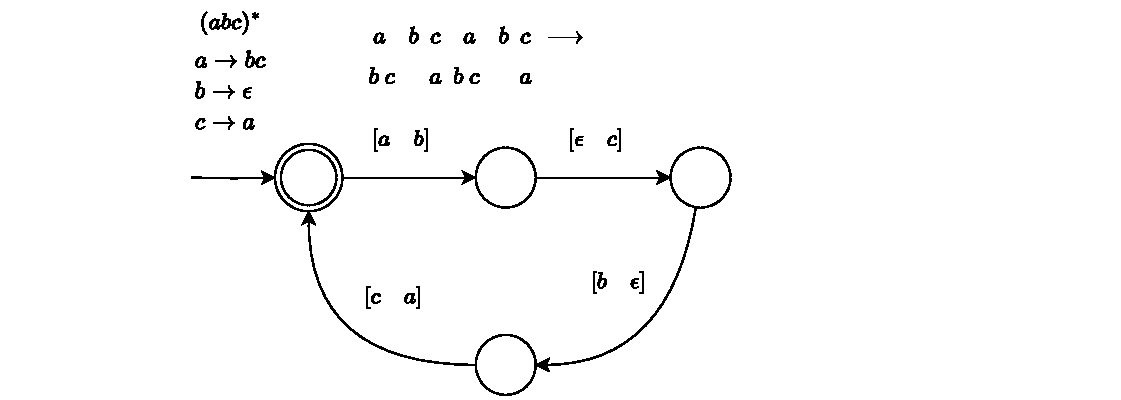
\includegraphics[scale=1.0, keepaspectratio]{obrazky-figures/transducer.drawio.pdf}
  \caption{
    Example of a 2-tape input/output \nft.
  }\label{fig:2_tape_nft}
\end{figure}

\end{example}

\section{Data Structure}
We propose utilizing the existing data structures in \mata (used for NFAs) for implementing finite transducers in \mata.
The main advantage is that NFAs, \nfts, and BDDs can all be implemented using the same single data structure, utilizing a lot of the existing algorithms on the data structures.

\mata provides a base class \nfaClass which encompasses both deterministic and non-deterministic finite automata and operations on them.
Class \nfaClass is a base class from which \nfts, BDDs, and register automata can inherit, including all operations on \nfaClass where only a few specific operations need to be modified for each respective type of finite-state machine.
This hierarchy also allows us to add model-specific operations to each type of automata without modifying operations for the other automata.
BDDs in our representation only extend the functionality of \nfts, and can therefore inherit most of the algorithms from \nfts and only modify some of the algorithms for BDD-specific use-cases.

\begin{figure}[ht]
  \centering
  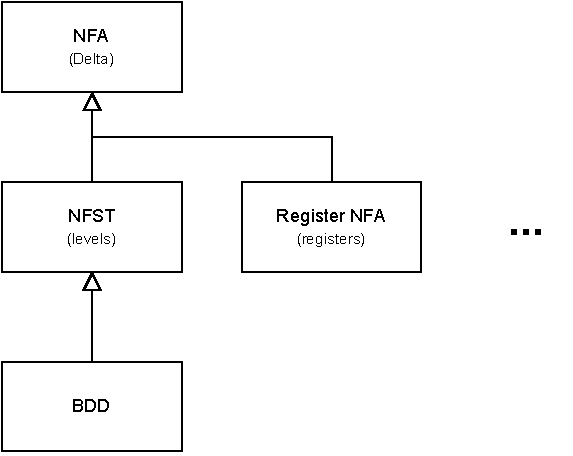
\includegraphics[scale=0.8, keepaspectratio]{jumps_synchronization-NFAs-NFSTs-BDDs-hierarchy.drawio.pdf}
  \caption{
    An inheritance hierarchy for NFAs, \nfts, BDDs, and register automata.
    All of these finite-state machines utilize the same data structure, with mostly the same algorithms where only a few algorithms needs to be modified for each respective type of finite-state machine.
    Each type of finite-state machine can further extend the set of operations by their own specific operations.
    Since BDDs only extend the functionality of transducers, BDDs can inherit directly from \nfts, modifying a few algorithms of \nfts together with the base \nfaClass algorithms.
  }
\end{figure}

Class \nfaClass defines which states in the represented automaton are initial (a set of initial states) and which are final (a set of final states).
Furthermore, \nfaClass allows for storing of arbitraty context in the automaton itself.

The most important data structure for the representation of the finite-state machines and the efficiency of the algorithms run on the representation is the representation of transition relation, called \deltastruct in \mata.
\deltastruct defines the set of states of the finite automaton, and gives the transition relation of the finite automaton.
\deltastruct is designed in such a way that often used operations such as iteration over transitions, adding and removing transitions, are performant, while less often used operations such as reversal of transition relation can be less performant.

States are in \mata represented as unsigned integers, numbered from 0.
This allows adding new states to the automaton to be as easy as getting the number of states in \deltastruct (constant time operation) and adding a number equal to the number of new states we want to add.
Such states are immediatelly allocated in \deltastruct and can be used in initial of final states sets.

Transition symbols are internally stored as unsigned integers as well, numbered from 0, where the last several unsigned integer values are reserved for epsilon symbols.
\mata provides several alphabet types which map the actual transition symbols to their internal values.

The use of unsigned integers for states and symbols gives implicit ordering over both states and symbols and querying them by accessing index corresponding to the internal state/symbol value in an ordered vector.
\deltastruct is a three-level data structure where each level represents one element from the three-tuple $(q, s, q')$ representing a single transition as:
\begin{enumerate}
    \item source states,
    \item transition symbols,
    \item target states.
\end{enumerate}

Each level is internally stored in memory as a sorted vector of unsigned integers, stored in a low-level data structure provided by \mata called \ordvector, a wrapper over \texttt{std::vector} maintaining a set of elements inserted to \texttt{std::vector} ordered.

\ordvector therefore has constant time access to stored elements, operations on the largest element (implemented internally as \texttt{push\_back()}, \texttt{pop\_back()}), fast linear iteration over the elements, and linear union, intersection, and difference.
Since vectors are ordered, lookup for states and symbols is logarithmic using binary search.
Insertion and removal of are logarithmic, but they must shift elements in the memory in the underlying \texttt{std::vector} which slows the operations down.

Due to this, \mata tries to iterate over \ordvector as often as possible since internally, \texttt{std::vector} stores elements in a continuous array on heap with good memory locality, and add elements one after the other in an ascending order given by the value of the inserted elements at the end of the ordered vector.
Several algorithms such as synchronized traversal over multiple ordered vectors.
General insertion and removal of transitions are logarithmic, but \mata algorithms are written in such a way that the general insertion and removal are seldom used.

This pairs well with underlying data structures for sets of initial and final states, implemented as sparse sets~\cite{sparseset93} allowing for constant element lookup, insertion and removal, and fast linear iteration through elements.

The Figure~\ref{fig:delta_struct} visualizes the three-level \deltastruct data structure. We can see that the when we access by source state $q$ the index in the first vector of source states, we get a vector post of type \statepost (\statepost[q]), representing $\post(q)$, which is a vector of symbol posts for each transition symbol $a$ leading from source state $q$, of type \symbolpost.
Each symbol post for symbol $a$ represents $\post(q, a)$, storing the transition symbol $a$ and a set of target states represented as a \ordvector.

% {\tiny
\begin{figure}[ht]
\begin{center}
% \includegraphics[width=10cm]{images/Delta.pdf}
% TODO: Replace with my own image of Delta struct.
\definecolor{color1}{RGB}{54,174,124}
\definecolor{color2}{RGB}{24,116,152}
\begin{tikzpicture}[
    circ/.style={draw,circle,inner sep=0pt,minimum size=2pt,fill},
    arr/.style={->,thick,>=stealth},
    type/.style={color2,dashed,thick},
    % >=stealth,
]

\matrix[
    matrix of nodes,
    nodes={draw, minimum size=5mm},
    % column sep=-\pgflinewidth,
    row sep=0.5mm,
    nodes in empty cells,
    row 1/.style={nodes={draw=none, fill=none, minimum size=5mm}},
% row 1 column 1/.style={nodes={draw}}
] (delta) {
0 & 1 & 2 & 3 & 4 & 5 & 6 & 7 & 8 & 9\\
  &   &   &   &   &   &   &   &   &  \\
};
\node[below = 0cm of delta-2-8,xshift=4.5mm] {\code{std{::}vector{<}StatePost{>}}};
\draw[decoration={brace,amplitude=10pt}, decorate, color1, thick] (delta-1-1.north west) -- (delta-1-10.north east) node [above = 10pt, pos=0.5] {Source states};
\draw[type] plot [smooth,tension=2] coordinates {($(delta.west)+(-2,-5)$) ($(delta)+(0,1.5)$) ($(delta.east)+(2,-5)$)};
\node[right = 1cm of delta,color2] {\code{Delta}};

\matrix[
    matrix of nodes,
    nodes={draw, minimum size=5mm, anchor=center, %text centered, align=center
    },
    % column sep=-\pgflinewidth,
    % row sep=0.5mm,
    % nodes in empty cells,
    below = 1.3cm of delta-2-6
] (statepost) {
$a$ & $c$ & $e$ & $r$ & $x$ & $\epsilon$ \\
};
\draw[arr] ($(delta-2-5.north west)!0.5!(delta-2-5.south east)$) node[circ]{} .. controls +(0,-.7) and +(0,0.7) .. (statepost-1-1.north west);
\node[below = 0cm of statepost-1-5] {\ordvector{}\code{{<}SymbolPost{>}}};
\node[above = 0cm of statepost-1-4, color1] {Transition symbols};
\draw[type] plot [smooth,tension=2] coordinates {($(statepost.west)+(-1.5,-2.5)$) ($(statepost)+(0,1)$) ($(statepost.east)+(1.5,-2.5)$)};
\node[right = 0.8cm of statepost,color2] {\code{StatePost}};

\matrix[
    matrix of nodes,
    nodes={draw, minimum size=5mm, anchor=center, %text centered, align=center
    },
    % column sep=-\pgflinewidth,
    % row sep=0.5mm,
    % nodes in empty cells,
    below = 1.3cm of statepost-1-2
] (symbolpost1) {
1 & 3 & 5 & 6\\
};
\draw[arr] ($(statepost-1-2.north west)!0.5!(statepost-1-2.south east)+(0.17,0)$) node[circ]{} .. controls +(0,-.7) and +(0,0.7) .. (symbolpost1-1-1.north west);
\node[below = 0cm of symbolpost1-1-3] {\ordvector{}\code{{<}State{>}}};
\node[above = 0cm of symbolpost1-1-3, color1] {Target states};
\draw[type] plot [smooth, tension=1.1] coordinates {($(symbolpost1.south west)+(-0.2,0)$) ($(statepost-1-2)+(0,0.15)$) ($(symbolpost1.south east)+(0.2,0)$)};
\node[right = 0.2cm of symbolpost1,color2] {\code{SymbolPost}};

\end{tikzpicture}

\end{center}
% \vspace{-6mm}
\caption{
The vizualization of the three-level data structure representing the transition relation of finite-state machine in \mata, called \deltastruct.
}
\label{fig:delta_struct}
% \vspace{-4mm}
\end{figure}
% }

Notice that since \mata supports epsilon symbols as maximal unsigned integer values, the symbol posts for epsilons are always at the end of state posts and can be therefore accessed in constant time instead of having to search the whole state post to look them up. \mata operations utilize this fact in numerous operations using epsilon symbols such as in string solving~\cite{fm23_equations_synergy_regular_constraints_DBLP:conf/fm/BlahoudekCCHHLS23}.

\nfts and BDDs can directly utilize \nfaClass with all of the underlying data structures where one transition in \nft is represented by several transitions in \nfaClass.
The only modification of \nfaClass to support \nfts and BDDs is adding a vector of state \emph{levels} (represented by \texttt{std::vector}<unsigned>) indexed by automaton states, as in the first level in \deltastruct. The vector maps each aumaton state to its level in the finite-state machine.
$n$-tape \nft has $n$ levels.
Therefore, in a representation of a $n$-tape \nft, vector of state levels maps to values from $0$ to $n-1$.
One transition in \nft corresponds to $n$ transitions in \nfaClass.

Each transition in \nfaClass corresponds to one level of the \nft, i.e., one tape of the \nft.
\nft transition always starts at level $0$. Transition from level $0$ to level $1$ represents the operation on the first \nft tape, from level $1$ to level $2$ the second \nft tape operation and so on.
Finally, the transition from state with level $n-1$ back to state with level $0$ corresponds to the last tape in the \nft.

For 2-tape (input/output) \nft, the levels used will be $0$ and $1$, where transitions from states with levels $0$ represent the input transitions and transitions from states with levels $1$ represent the output transitions.

We denote a level $l$ of a state $x$ as $l = \level{x}$.
In this work, we use terms \emph{level} and \emph{tape} interchangeably.

For this reason, \nfts can have as initial or final states only states with state level $0$.
This is crutial for many algorithms (more in~\ref{sec:Algorithms}) which rely on certain invariants in the representation of \nfts, such as that \nfts always synchronize in states with state level $0$ and each step in operations must consider the entire state levels sequence from $0$ to $n-1$ as a single \emph{abstract} step.

\subsection{Epsilon and Don't Care Transitions}

\nfts and BDDs also need suport for epsilon symbols and don't care symbols on transitions.

\mata already supports epsilon symbols as (several) last transition symbol(s) in the range of possible transition symbols given by the data type of transition symbol.
Adding support for \emph{don't care} symbols on transitions, matching any transition symbol on the tape.

An epsilon symbol on a transition from state with level $k$ to level $k + 1 \% n$ in \nfaClass representing a \nft means that the tape corresponding to the level $k$ does not read from / write on the tape $k$ any symbol.

\nfts represented as \nfaClass also require support for \emph{jumps} where the transition goes from a state with level $k$ to any other state with level $l$ where $l \neq k + 1$.
However, we restrict the jumps for $n$-tape \nft as follows:
\begin{itemize}
  \item The jump cannot jump over a state with level $0$.
  That is, if we need to jump further, the transition can at most jump to the next state with level $0$,
  \item A jump of length $k$ greater than one (the length of one is a normal transition in \nfaClass which we call just a transition) is interpreted the same as if we made $k$ transitions in \nfaClass with the transition symbol on the jump transition.
  That is, a jump of length $3$ (over $3$ tapes) with transition symbol $\epsilon$ means that the transducer made $3$ normal transitions with $\epsilon$ as a transition symbol for each of them.
  \item Jumping from a state with level $0$ to the next state with level $0$ means that only the internal state of the \nft has changed (the state has changed) without reading or writing anything on any of the tapes.
\end{itemize}

% TODO: Figure for jumps.




\begin{example}\label{example:2_tape_nft_in_mata}
  The \nft from Example~\ref{example:2_tape_nft} is represented in the data structure for \nfts inherited from \nfaClass as in the Figure~\ref{fig:2_tape_nft_in_mata}.

  Transitions from states with level $0$ represent the input tape transition symbol, and transitions from states with level $1$ represent the output tape transition symbol.

  \begin{figure}[ht]
    \centering
    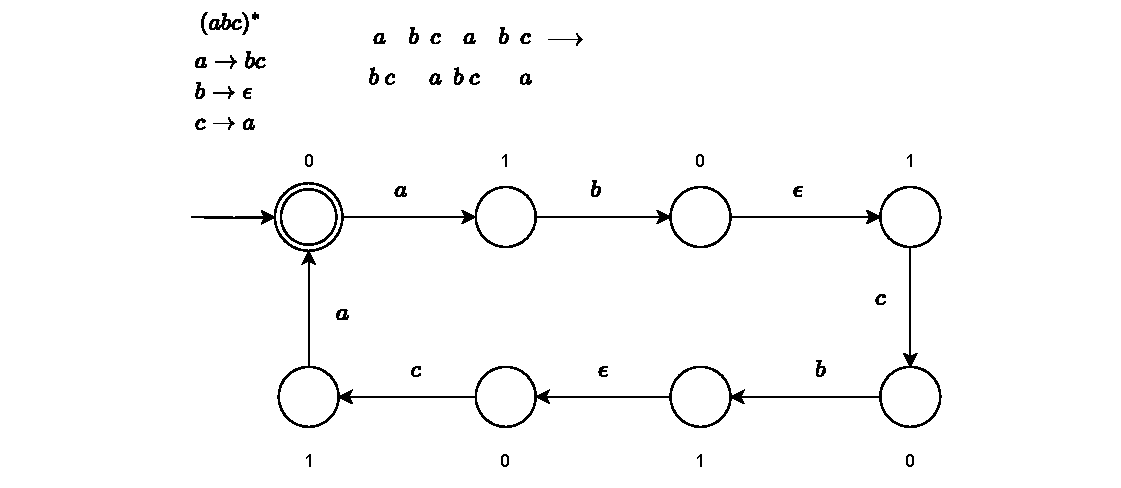
\includegraphics[scale=1.0,keepaspectratio]{obrazky-figures/transducer_in_mata.drawio.pdf}
    \caption{
      2-tape \nft from Example~\ref{example:2_tape_nft} represented in \mata as an \nfaClass with states annotated by levels.
    }\label{fig:2_tape_nft_in_mata}
  \end{figure}
\end{example}

\subsection{No Operation Transitions}
An epsilon transition from a state with level $k$ to $k+1 \mod n$ can be understood as a \emph{no operation transition} \nop, i.e., a transition where the current tape does not perform any operation (no reading nor writing). In essence the impact of the transition is the same as if reading an empty string on the current tape.

In constrast, an epsilon transition from a state with level $k$ to another state with level $k$ is a simple change of states (as per the usual definition of epsilon transitions in \nfas).

Depending on the application, one might prefer to use one or the other representation as needed.
In this work, we use \nop when we want to explicitly stress the distinction between a simple change of state in \nft (an epsilon transition between states with the same level), and no operation on a current tape (tape does not read nor writes any symbol).

\section{Algorithms}
\label{sec:Algorithms}

For general uses of transducers in \mata, we have implemented general automata operations for creating, modifying, and manipulating transducers.
Furthermore, we have implemented several transducer-specific operations.

\paragraph{\nfa operations.}
The general \nfa operations such as concatenation, union, etc. can be reused from \nfa without many modifications.
We only need to remember to correctly set levels of states when renumbering states in the result \nft.

Further, we discuss several more significant modifications to existing operations and algorithms for several \nft-specific operations.

\subsection{Synchronization}

All operations performing some kind of traversal over the transitions start the compution from states with level $0$.
\nfts are always synchronized on states with level $0$, that is, after each \nft transition is completed (all tape operations are handled).
If the macrostate in a worklist contains only states of multiple \nfts with levels $0$, the \nfts are synchronized and the next macrostate can be computed.
When the synchronized \nfts perform one transition, due to the supported jumps, the new macro state may contain states with different levels.
Only the state in the macrostate with the level furthest behind is expanded (performs its transitions, if possible).
The others are at least one level ahead and therefore cannot be expanded and must wait for the states behind to get to at least their levels first before being expanded themselves.

Since jumps can jump at most to the next state with level $0$, we always know which states in the macrostate are ahead and which are behind by the following method.
If we expand a macrostate with states with levels $k$ and $l$ where $k > l$, we know that state with level $k$ must be ahead of the state with level $l$.
If any of the states has level $0$ (and there are other states with nonzero levels), we know that the state $0$ must be ahead of all the other states with nonzero levels, and synchronized with all other states with levels $0$.
That holds since the states with levels $0$ can only be the next states with levels $0$, and not the states with level $0$ behind (as the first step from the synchronized states is to move immediately out of the states with level $0$ behind).

The same holds for BDDs utilizing the same data structure and constraints as \nfts.

\begin{example}
  If we perform synchronization over three $4$-tape \nfts, starting from macrostate with levels $(0, 0, 0)$, we perform one transition and may end up in a macrostate with levels $(3, 1, 0)$ where the first \nft made a jump of length $3$, the second performed normal transition (jump of length $0$), and the last \nft performed a jump to the next state with level $0$.
  When expanding the macrostate $(3, 1, 0)$ later on, we know that the state with level $0$ is ahead of the other states with levels $3$ and $1$. And we further know that state with level $3$ must be ahead of the state with level $1$. Therefore, the state with level $1$ must be expanded up until the level reaches $3$ or greater (the next level $0$).
  Then we may get $(3, 3, 0)$, both the first and the second state are expanded to states with levels $(0, 0, 0)$ and the macrostate is synchronized again.
\end{example}

\begin{figure}[ht]
  \centering
  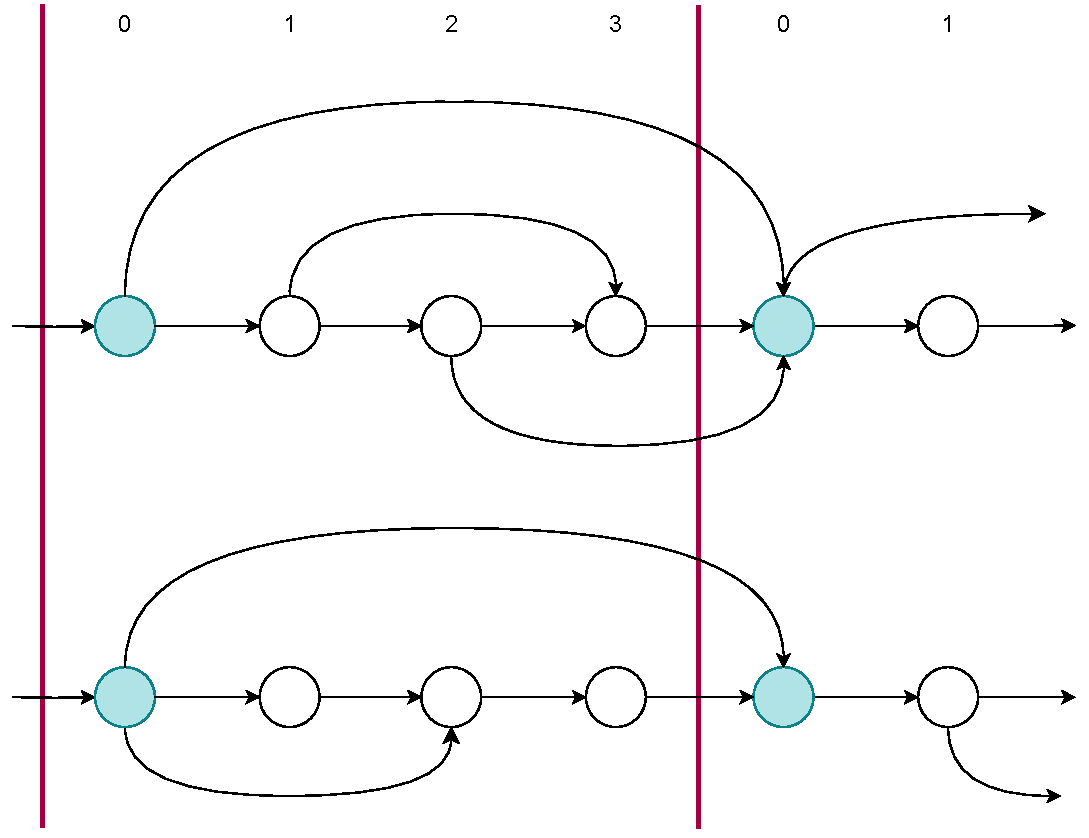
\includegraphics[scale=0.5, keepaspectratio]{obrazky-figures/jumps_synchronization.drawio.pdf}
  \caption{
    An example of allowed jumps in $4$-tape \nfts during synchronization.
    Jumps can start in state with any level and jump up to the next state with level $0$.
    The jumps cannot jump over states with level $0$, however.
    The numbers denote the levels for the corresponding states below.
    The highlighted states depict the states with level $0$, the vertical lines visually set apart \nft transitions (there is one \nft transition, consisting of several tapes, between each pair of vertical lines).
  }

\end{figure}

\paragraph{Alternative representation of jumps.}
If the restriction of allowed jumps being only to the next state with level $0$ is too strict, an alternative approach where jumps are allowed to jump over (potentially multiple) states with level $0$ can be chosen.
However, during operations such as product construction, an additional information must be added to the worklist containing macrostates containing a list of lengths of each jump performed during the expansion of the last macro state in order to know how far ahead are the states jumped to in relation to the other states in the macrostate.

We deem this approach inferior to our chosen approach since it distorts the simplicity of a single data structure and algorithms on it for NFAs, \nfts, and BDDs.

% ==================================
\subsection{Projection}\label{sec:projection}

The first standard operation on transducers is \emph{projection}.
Given an $n$-tape \nft $\ft$, we can perform \emph{projection to} a specified set of tapes, or \emph{project out} a specified set of tapes.

The transitions remain the same, the only change is that we remove certain tapes (meaning that for every \nft transition we remove transition symbols on those tapes).
In \mata, this means removing all states with certain levels $k$ and their outgoing transitions and redirecting ingoing transitions to these states to the next states with levels $k + 1 \mod n$ where the outgoing transitions were previously leading to.
This can be iteratively performed on all tapes specified for removal.
When the modification is performed, all remaining levels are shifted toward $0$ to start at $0$ and end with $l - 1$ where $l$ is the new number of tapes remaining in \nft.

Projection to, denoted $\projToSet{M}{\ft}$ where $M \subseteq \{ 0, 1, \ldots, n - 1 \} $ is an operation which removes from $\ft$ all other tapes $o \notin M$ and keeps only those tapes $t \in M$.
In practice, this means that an $n$-tape \nft will be modified into an $|M|$-tape \nft.
If $|M| = 1$, we create a $1$-tape \nft (containing only states with level $0$) which is semantically equivalent to a corresponding \nfa with the same transitions.

Projection out, denoted $\projOutSet{M}{\ft}$, performs the same operation, only now instead of keeping the specified tapes $o \in M$, we remove all tapes $o \in M$, and keep only the tapes $t \in \{ 0, 1, \ldots, n - 1 \} \setminus M$.
If $|M| + 1 = n$, we project out all tapes except for one.
This creates a $1$-tape \nft, which is again semantically equivalent to a corresponding \nfa with the same transitions.

Note that for either variation, removing the first tape in \nft transitions requires setting new initial states (the original targets of transitions from the states with level $0$ become the new initial states).
Similarly, removing the last tape in \nft transitions requires setting new final states (the original source of ingoing transitions to the final states become the new final states).
If jump transitions are involved, one may need to expand the jumps into normal transitions between levels to set the correct initial and final states on the new first and last tape.

\begin{example}
  Given an \nft $\ft$ with $5$ tapes, with levels $\{ 0, 1, 2, 3, 4 \}$.

  We can perform the following operations:
  \begin{itemize}
    \item $\projOutSet{\{ 3 \}}{\ft}$ which deletes tape $3$ from $\ft$, leaving tapes $\{ 0, 1, 2, 4 \}$ which are then renumbered to $\{ 0, 1, 2, 3 \}$.
    \item On the result, we can perform $\projToSet{\{ 1, 3 \}}{\ft}$ which performs the same as if calling $\projOutSet{\{ 0, 2 \} }{\ft}$.
    Tapes $0$ and $2$ are removed, leaving tapes $\{ 1, 3 \}$, which are then renumbered to $\{ 0, 1 \}$.
    \item Now, peforming $\projToSet{\{ 1 \}}{\ft}$ gives us \nft with only one tape, which represents the \nfa for the tape $1$.
    Performing $\projOutSet{\{ 1 \}}{\ft}$ instead would give us \nft with only one tape representing the \nfa for the tape $0$.
  \end{itemize}

\end{example}

% ==================================
\subsection{Intersection}\label{sec:intersection}

For constructing the intersection of two \nfts, we make use of the inheritance of \nfts from \nfas and utilize the classical intersection computation on \nfa using the standard product construction algorithm (as described in Chapter~\ref{sec:Preliminaries}).
The only modification is adding support for proper assignment of levels to new macrostates depending on the levels of the original \nft states in the macrostate, and handling of various combinations of transition symbols during the process of adding transitions leading from the macrostates.

Given $\ft_1$ with $\states_1$ and $ft_2$ with $\states_2$, construct the intersection of $\ft = \ft_1 \cap \ft_2$.

A new level $\level{q'}$ for a new macrostate $q' = (q'_1, q'_2)$, given a current macrostate $q = (q_1, q_2) \in \states_1 \times \states_2$ where $q'_1$ and $q'_2$ are targets of transitions from $q_1$ and $q_2$, is determined as follows:
\begin{itemize}
  \item If $q'_1 = 0$ or $q'_2 = 0$ (holds for both equal $0$, too), $\level{q'} = \texttt{max}(\level{q'_1}, \level{q'_2})$. If both target states have levels $0$, we are finishing an entire \nft transition and enter a synchronized macrostate $q'$, $\level{q'} = 0$. Otherwise, only $q'_1 = 0$ ($q'_2 = 0$) holds, and $q'_1$ ($q'_2$) must be "further ahead" of $q'_2$ ($q'_1$), and must wait for $q'_2$ ($q'_1$) to catch up, therefore, $0 < \level{q'} < n$.
  \item Otherwise, $\level{q'} = \texttt{min}(\level{q'_1}, \level{q'_2})$. That is, if both $0 < \level{q'_1}, \level{q'_2} < n$, we must wait for the state further behind to catch up, so we choose the lower level as $\level{q'}$.
\end{itemize}

A new transition symbol $a \in Sigma$ for a new transition $(q, a, q')$ is chosen by the following rules:
\begin{itemize}
  \item If $(q_1, a, q'_1) \in \post_1$ and $(q_2, a, q'_2) \in \post_2$, $(q, a, q') \in \post$.
  \item If $(q_1, \epsilon, q'_1) \in \post_1$ and $(q_2, \epsilon, q'_2) \in \post_2$, $(q, \epsilon, q') \in \post$. Epsilon symbols are handled here as normal symbols $a \in \Sigma$. This ensures that only matching $\epsilon$ symbols are synchronized.
  \item If $(q_1, \dontCare, q'_1) \in \post_1$ (or $(q_2, \dontCare, q'_2) \in \post_2$), $a$ from $(q_2, a, q'_2)$ ($(q_1, a, q'_1)$) is used.
  This holds for $(q_1, \dontCare, q'_1) \in \post_1$ and $(q_2, \dontCare, q'_2)$, too.
  This works if one of the symbols is $\dontCare$ and the other is $\epsilon$, too: $(q, \epsilon, q')$ is produced in such a case.
\end{itemize}

The rules are visualizated in the Table~\ref{tab:synchronization_rules}.
\begin{table}[ht]
\centering
\begin{tabular}{ |c||c|c|c|c| }
 \hline
 $\cap$ & $\dontCare$ & $\epsilon$ & a & b \\
 \hline
 \hline
 $\dontCare$ & $\dontCare$ & $\epsilon$ & a & b \\
 \hline
 $\epsilon$ & $\epsilon$ & $\epsilon$ & & \\
 \hline
 a & a &  & a &\\
 \hline
 b & b &  & & b\\
 \hline
\end{tabular}
\caption{
  Synchronization rules for transitions symbols during intersection.
  The row lists the symbols on transitions in $\ft_1$, the column in $\ft_2$.
}
\label{tab:synchronization_rules}
\end{table}

Finally, $\dontCare$ transitions must be handled separately since the classic intersection algorithm does not match $\dontCare$ with any other symbol than $\dontCare$.

% ==================================
\subsection{Composition}

When working with \nfts as transduction machines taking some input, modifying it and outputting some output, we often encounter problems where we want to perform multiple transductions on the input, one after the other.
In the same way as we can compose mathematical functions $(f \circ g)(x)$ meaning $f(g(x))$ (perform $g$ on $x$ and perform $f$ on the result of $g(x)$),
we can perform multiple \nfts transductions sequentially: $\ft_2 \circ \ft_1$
(perform the transduction of $\ft_1$ on the input, and then perform the transduction of $\ft_2$ on the result), denotes as $\compose{\ft_1}{\ft_2}$.
Using the Unix \emph{pipe} notation, we can express the same with $\ft_1 \composePipe \ft_2$
(perform the transduction of $\ft_1$ on the input, and then pipe the result to $\ft_2$ to perform the transduction of $\ft_2$ on the result).

For each \nft, we need to specify which tape(s) $T$ to synchronize on with the other \nft.
This are the tapes we expect to act as a mediator between the output of $\ft_1$ and the input of $\ft_2$.
To create a new product transition, the symbols on the corresponding tapes in both \nfts must be compatible (the same symbol, or pairs like $(\dontCare, a)$ for $a \in \Sigma$, etc.).
% TODO: Explain synchronization better.

\begin{example}
  Throughout this section, we will demonstrate the composition algorithm on the following example.
  Given \nft $\ft_1$ with tapes $0$, $1$, and $2$, and $\ft_2$ with tapes $2$, $3$, $4$, we want to compute $\ft_1 \composePipe \ft_2$, synchronizing both \nfts on tape $2$.
  For clarity, we number the tapes uniquely between both \nfts in this example. Internally, each \nft has tapes with levels from $0$ to $2$ and for each \nft, we specify which tape(s) the \nfts should synchronize on.
\end{example}

The composition comprises the following steps:
\begin{itemize}
  \item Extending the \nfts to contain matching tapes,
  \item Adding special self-loops on states with level $0$ to allow for proper handling of $\epsilon$ and $\dontCare$ symbols on the transitions,
  \item Performing \nft intersection as described in Section~\ref{sec:intersection}, and
  \item Projecting out the synchronization tapes (as described in Section~\ref{sec:projection}) which were "consumed" by the composition.
\end{itemize}

\paragraph{Extending \nfts to match each other.}
The first step of the composition is to extend the input \nfts by inserting additional levels $k$ (additional states with levels $k$) into each transition with $\dontCare$ symbols on the transitions at levels $k$.
This operation balances out the \nfts so both have the same tapes in the same order.
This allows us to perform the classic \nfa intersection for each level in both \nfts during \nft intersection.
We use $\dontCare$ symbols since for each \nft $\ft_i$, the other \nft $\ft_j$ does not care what transitions over what symbols $\ft_i$ performs during the intersection.
Hence, from the point of view $\ft_j$, $\ft_i$ can perform any transition.

\begin{example}
  Continuing the example, we extend each \nft transition in $\ft_1$ with $\dontCare$ transitions from existing states with level $2$ to new states with levels $3$, from states with levels $3$ to new states with levels $4$, and finally from states with levels $4$ to the next existing states with levels $0$ (finishing the original \nft transition) which were the original targets of transitions from states with levels $2$.

  Figure~\ref{fig:composition_nfts_extension} shows a depiction of a single transition in $\ft_1$ and $\ft_2$ before and after extension.

  \begin{figure}[ht]
    \centering
    \subfloat[\centering Before extension\label{fig:composition_nfts_extension_before}]{{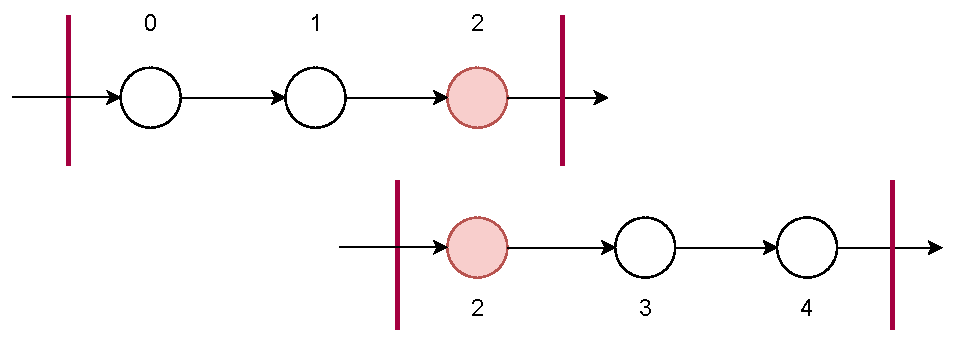
\includegraphics[keepaspectratio,width=0.45\textwidth]{jumps_synchronization-composition_nfts_extension.pdf} }}%
    \qquad
    \subfloat[\centering After extention\label{fig:composition_nfts_extension_after}]{{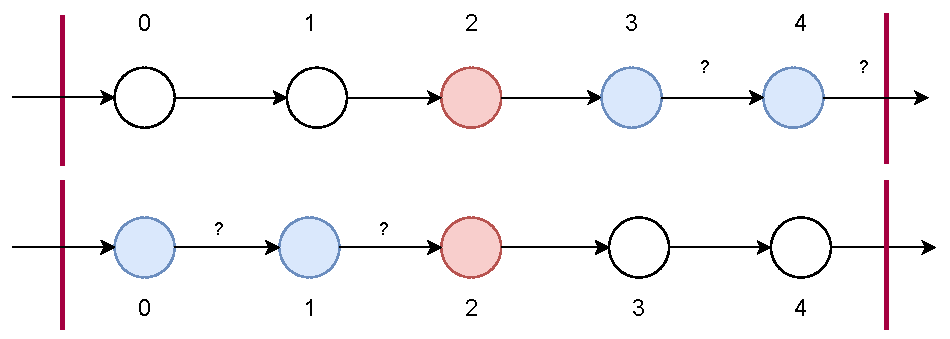
\includegraphics[keepaspectratio,width=0.45\textwidth]{jumps_synchronization-composition_nfts_extension_balanced.pdf} }}%
    \caption{
      A depiction of a single transition in \nfts $\ft_1$ (top) and $\ft_2$ (bottom) before extension (Figure~\ref{fig:composition_nfts_extension_before}) and after extension with $\dontCare$ transitions on inserted tapes to balance out the tapes in both \nfts (Figure~\ref{fig:composition_nfts_extension_after}).
      The red states with together with the outgoing transition represent the tape $\ft_1$ and $\ft_2$ are synchornized on.
      The blue states represent the newly inserted tapes with $\dontCare$ symbols on transitions.
    }
    \label{fig:composition_nfts_extension}%
  \end{figure}

  We can see that after the extension, both $\ft_1$ and $\ft_2$ have the same tapes.
\end{example}

Thanks to this general approach, we can compute compositions of any $n$-tape \nfts\footnote{Where $\ft_1$ and $\ft_2$ does not even have to have the same $n$.}, synchronizing on any tape(s)\footnote{When synchronizing on multiple tapes, the tapes must at least be in the same order in both \nfts.}, with the tapes being in an arbitrary order.

As an optimization, when adding multiple subsequent $\dontCare$ transitions during the extension, we can instead add only a single $\dontCare$ jump from the first state in the sequence leading to the last state in the sequence, without having to create new states for all inserted tapes being jumped over.

\paragraph{Adding self-loops.}
The next step is to add self-loops to all states with level $0$ in both \nfts.
These self-loops serve the purpose of nondeterministic "waiting" loops for waiting at the beginning of an \nft transition in one \nft for the other \nft for epsilon transitions on the tapes being synchronized on.

The self-loops is a symbolic name since they are self-loops in the sense of \nft transitions (from state with level $0$ back to the same state), but they lead over several tapes (i.e., several states with transitions).

The symbols on the self-loops are added as follows:
\begin{itemize}
  \item For the transitions on tapes $T$, the symbol is $\epsilon$ is used, being handled as a normal transition symbol the other \nft can synchronize with an $\epsilon$ symbol on the non-self-loop transition.
  \item For the transitions on tapes added by the extension, the symbol is $\dontCare$ is used.
  $\dontCare$ here has the same role as $\dontCare$ symbols added during extension.
  \item For the transitions on the remaining tapes (the original non-synchronizing tapes), $\epsilon$ symbol is used to represent the waiting on all \nft's own transitions.
\end{itemize}

\begin{example}
  Figure~\ref{fig:composition_nfts_extension_loops} shows how a single transition in \nfts looks after adding the "waiting" self-loops.
  \begin{figure}[ht]
    \centering
    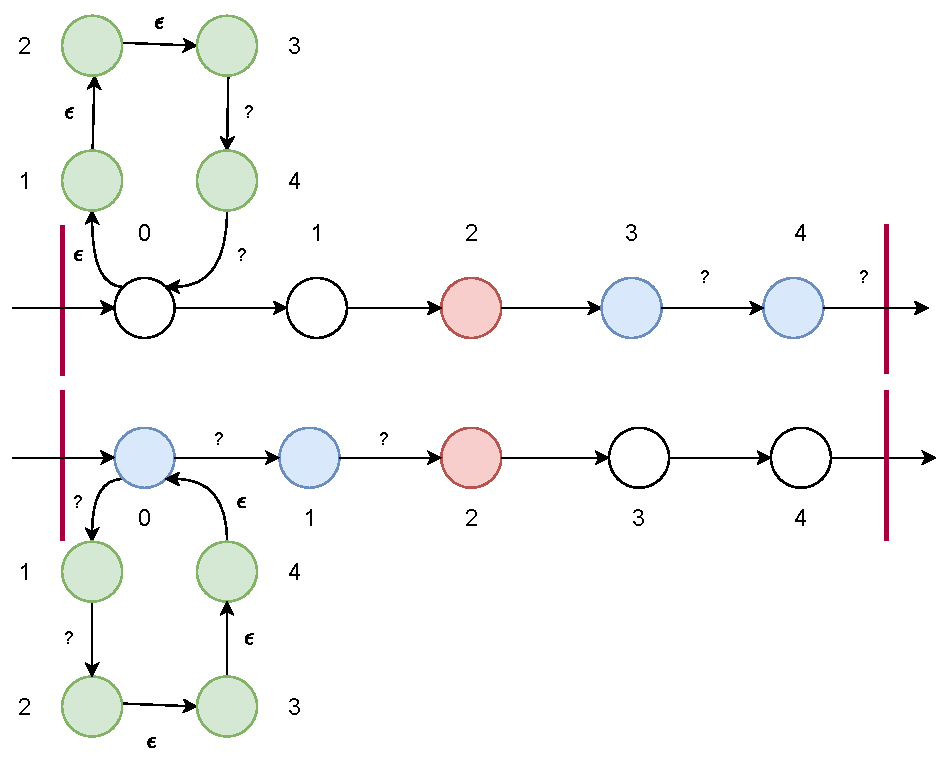
\includegraphics[keepaspectratio, width=0.5\textwidth]{jumps_synchronization-composition_nfts_extension_loops.pdf}
    \caption{
      A depiction of a single transition in \nfts $\ft_1$ (top) and $\ft_2$ (bottom) after adding the "waiting" self-loops.
    }
    \label{fig:composition_nfts_extension_loops}
  \end{figure}
\end{example}

\paragraph{Intersection.}
When the \nfts are balanced out and self-loops are added, we can perform an \nft intersection, as per Section~\ref{sec:intersection}.
The intersection produces a new \nft representing the composition of $\ft = \ft_1 \composePipe \ft2$, only currently $\ft$ still contains all the tapes from the balanced $\ft_1$ and $\ft_2$.
Other that that, the composition is complete.

Note that since we added the self-loops, we no longer need to separately handle $\epsilon$ transitions.
$\epsilon$ symbols are handled as normal transitions, producing an $\epsilon$ transition in the product iff both \nfts perform an $\epsilon$ transition, or one of them performs a $\dontCare$ transition.

Furthermore, we prevent self-loops in both \nfts from synchronizing with each other.
 That is, we cannot construct a new macrostate $q' = (q_{l1}, q_{l2})$ where both $q_{l1}$ and $q_{l2}$ are self-loop states.
This would represent a situation where both \nfts are waiting for the other, but none moves forward.
Since these macrostates are not useful, we prevent their creation entirely.

\paragraph{Projecting out the tapes the composition synchronized on.}
To clean up $\ft$, we need to project out the tapes $T$ we synchronized on as these are the tapes that have been "consumed" by the composition.

\begin{example}
  To finish out example, Figure~\ref{fig:composition_nfts_extension_final} depicts a single product transition after composition is performed and the synchronization tapes are projected out.
  \begin{figure}[ht]
    \centering
    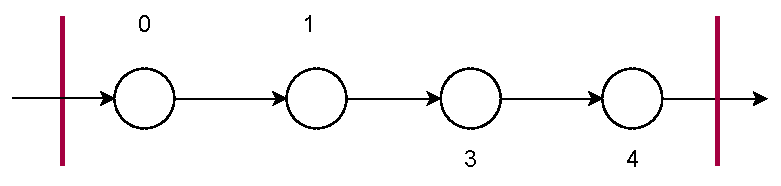
\includegraphics[keepaspectratio, width=0.5\textwidth]{jumps_synchronization-composition_nfts_extension_final.pdf}
    \caption{
      A depiction of a single product transition in $\ft = \ft_1 \composePipe \ft_2$ synchonized on tape $2$.
      The levels at the top represent the original tapes before renumbering.
      The levels at the bottom represented the final tapes after renumbering.
    }
    \label{fig:composition_nfts_extension_final}
  \end{figure}
\end{example}

\paragraph{Optimization for $2$-tape \nfts.}
For working with only $2$-tape \nfts, a specialized algorithm for composition can be utilized.
The algorithm would still utilize the general idea of \nft intersection, but now no extension of \nfts and no self-loops are necessary.
For each macrostate, we would first perform a step in $\ft_1$ on level $0$, then perform the synchronized step on levels $1$ in $\ft_1$ and $0$ in $\ft_2$ (if such a step is possible as per \nft intersection rules), then finish the composition of the current transition by performing a step in $\ft_2$ on level $1$, constructing a new macrostate from targets of transitions on levels $1$ of both \nfts.
Handling of jumps is similar to \nft intersection: waiting for the state "left behind" to catch up with the state jumped to.

When adding support for transducers to \noodler, it may be advantageous to utilize this specialized variation of composition as string replace operations in \noodler only ever work with $2$ tapes.

% ==================================
\subsection{Application}

When we construct an \nft $\ft$, the most intuitive use of $\ft$ is to perform the transduction (the process of reading the input on input tapes and outputting the output on the output tapes) $\ft$ encodes.
This operation is called \emph{Application}.

We can \emph{apply} a word $w$ on $\ft$, or a regular language $\langof{\aut}$ for some $\aut$.

\paragraph{Application of a word.}
We can either apply a word $w \in \Sigma^*$ on a given tape (at level $k$), or apply an $l$-tuple of words $(w_i)$ where $i in \in \{ 1, \ldots, n \}$ where $|(w_i)| = l$ and $i$ specifies on which tapes we want to apply the tuple of words (one word $w_i$ for each tape $i$).

The result of the application of a word (or a tuple of words) is a set of tuples of size $(n - l)$ of words.
We read the word(s) being applied and move through the \nft according to the transition symbols in the applied word(s) on the corresponding tapes, similarly to performing a run on a word in \nfa, only now to potentially multiple tapes (multiple words).
During the traversal, we construct the result by appending the transition symbols on the remaining tapes to the result constructed so far for the current state.
This gives us the corresponding word on the remaing tapes when the words on the given tapes are $(w_i)$.

Focusing on $2$-tape \nfts $\ft$, the application equals to translation from the input word $w$ to the output word $w'$ (similarly to what a natural language translator does) where $w' = \apply{\ft}{w}$.
By convention, we presume the input tape is at level $0$ and the output tape is at level $1$.

The application of a word is equivalent to $\idNft{\aut} \composePipe \ft$ where $\aut$ represents a \dfa accepting only $w$.
This gives us an \nft encoding the result.
For $2$-tape $\ft$, we get a $1$-tape \nft, equal to the corresponding \nfa encoding the set of words in the result.

\paragraph{Application of a language.}
Applying a regular language $\langof{\aut}$ on $n$-tape \nft $\ft$ instead of a single word is performed similarly to the application of a single word, but now the result is a regular language (for $2$-tape \nfts) or an \nft $\ft'$ with $n-1$ tapes.

The application of a language $\langof{\aut}$, similarly to the application of a word, is equivalent to $\idNft{\aut} \composePipe \ft$.
The resulting \nft encodes the result.
For $2$-tape $\ft$, we get a $1$-tape \nft, equal to the corresponding \nfa encoding the regular language of the result.



% Basic approach, operations, representation
\chapter{Finite Transducers for String Solving}

SMT String solving is a complex and diversive problem which has seen a lot of interest over the past few decades.
Many different approaches for reasoning about word equations, word disequations, regular constraints, and length constraints have emerged, be it as a theoretical work, or implemented directly in one or more of the current state-of-the-art SMT string solvers, e.g.,~\cite{cvc4,cvc5,z3,Z3-str,Z3Str3,Z3str4,Trau,fm23_equations_synergy_regular_constraints_DBLP:conf/fm/BlahoudekCCHHLS23, tacas24_noodler_10.1007/978-3-031-57246-3_2, oopsla23_stabilization_DBLP:journals/pacmpl/ChenCHHLS23}.
Each invented approach and each string solver brings a unique set of features and advantages.

We decided to try a novel approach in \noodler, entirely different from other state-of-the-art SMT string solvers (except for \ostrich).
\noodler utilizes finite automata to encode the SMT formulae into a set of regular language constraints where the operations on finite automata as well as the representation of the finite automata themselves is handled by \mata.
This approach gives \noodler a unique oportunity to efficiently encode several problems in string solving as operations on finite automata which other string solvers cannot utilize.

Finite automata can encode regular languages, but string solving problems work with various SMT operations, where some of them cannot be easily encoded into only regular languages.
Such examples are regular replacement operations, namely \texttt{str.replace}, \texttt{str.replace\_re}, \texttt{str.replace\_all} and \texttt{str.replace\_re\_all} from the theory of strings in SMT-LIB~\cite{smtlib_theory_strings}.
However, finite transducers naturally encode rational relations between regular languages which can be directly utilized to encode such problematic SMT operations while allowing for efficient automata (transducer) operations on the relations and languages.

If \noodler could utilize finite transducers in a similar fashion to how it utilizes finite automata in its decision procedure, these SMT operations would be easy to compute and integration of finite transducers into its decision procedure would be a natural extension of the existing decision procedure.

Thus, we discuss in this chapter how to utilize finite transducers in \noodler to solve SMT string constraints \texttt{str.replace}, \texttt{str.replace\_re}, \texttt{str.replace\_all} and \texttt{str.replace\_re\_all}.

\section{Replace Operations}
A general regular replacement operation has the following form:
\begin{center}
\begin{verbatim}
  replaced_string = replace(input_string, pattern, replacement)
\end{verbatim}
\end{center}
where \texttt{replace} determines the type of the regular replacement (the semantics of the replacement operation).
\texttt{input\_string} represents the original input string where we want to replace some regular \texttt{pattern} with a \texttt{replacement} literal.
Regular \texttt{pattern} can be a string literal (a word) or a regular language describing the substring (or substrings) of \texttt{input\_string} we are trying to replace.

There are various replacement semantics for replace operations. Popular regular replacement types are \emph{reluctant replacement}, \emph{greedy replacement}, or \emph{possessive replacement}, or \emph{declarative replacement}.
For example, reluctant replacement matches a given \texttt{pattern} (a regular language) with the shortest substring of the \texttt{input\_string}, while the greedy replacement matches the longest substring. These types produce the same result when \texttt{pattern} is a string literal.
Possessive replacement semantics is that of the greedy one, but without backtracking on the substring matched so far.
Declarative replacement matches every occurrence of regular \texttt{pattern} in the given \texttt{input\_string}.

In opposition, \emph{procedural} regular replacements encompass the greedy and reluctant replacements since both match in \texttt{input\_string} from the left to the right.
The start with the first character in the word and by using backtracking continue through the word until the end of the word.

Since SMT-LIB defines only replacement operations of type reluctant replacement with the left-most matching and other types of the replacement operations are not allowed in SMT formulae in SMT-LIB format (which \noodler solves), we focus in this work solely on the reluctant replacement type.

We denote reluctant regular replacement as $x_{\pi \rightarrow y}$ as where $x$ is the \texttt{input\_string}, $\pi$ is the regular \texttt{pattern} (a literal or a regular language) and $y$ is the \texttt{replacement}.

\section{Encoding Reluctant Regular Replacement as Finite Transducers}

SMT-LIB suports two types of reluctant replacements: a \emph{reluctant all replacement} which replaces all occurrences of the shortest left-most matches of \texttt{pattern}, and \emph{reluctant single replacement} which replaces only the first shortest left-most occurrence of \texttt{pattern}.

\paragraph{Epsilon in \texttt{pattern}.}
If the \texttt{pattern} contains epsilon symbol, a special handling of epsilon matching needs to be performed. In such a case, one encodes the replacement operation as if $\epsilon \notin \pi$, and solves the replacement for two options:
\begin{itemize}
  \item Tries solving for just $\epsilon$ manually, and alternatively
  \item Solves the reluctant replacement without the epsilon if the $\epsilon$ match fails.
\end{itemize}
Since SMT-LIB works only with reluctant replacements, the reluctant replacement would always pick the shortest replacement, i.e., the $\epsilon$ replacement. The reluctant match of $\epsilon$ will always succeed and longer matches will not be needed nor accepted. SMT-LIB declares results to such patterns with $\epsilon$ to be equal to $\texttt{replacement} \concat \texttt{input\_string}$ (prepending the replacement to the \texttt{input\_string}).

% Define reluctant replacement.

\begin{definition}[\textbf{Reluctant all replacement}] \hfill \newline
  A \emph{reluctant all replacement} $x^{+}_{\pi \rightarrow y}$ is defined as follows: \newline
  $$x^{+}_{\pi \rightarrow y} = \{ u \concat y \concat w^{+}_{\pi \rightarrow y} \} \text{,}$$
  where $u, v, w, x, y \in \Sigma^*$, $\pi$ is a regular language (regex), $x = u v w$, $u \notin \Sigma^* \pi \Sigma^*$, $v \in \pi$, and to ensure the shortest left-most matching, the following must hold: $\forall u = u_1 u_2, v = v_1 v_2, w = w_1 w_2:$ if $v_2 \neq \epsilon$ then $v_1 \notin \pi$ (the shortest match as if $v_1$ is not a match, then surely the  shortest match is $v = v_1v_2$); if $u_2 \neq \epsilon$ then $u_2 v_1 \notin \pi \land u_2 v w_1 \notin \pi$ (the left-most match is $v$ since there is no match of $\pi$ before $v$).
\end{definition}

A reluctant single replacement is defined similarly, only the recursive replacement of $w$ is no longer performed since after the first replacement of $v$, no more patterns matchings are tried on the substring $w$ after the replaced substring $v$.
\begin{definition}[\textbf{Reluctant single replacement}] \hfill \newline
  A \emph{reluctant single replacement} $x^{1}_{\pi \rightarrow y}$ is defined as reluctant all replacement, only with the recursive replacement removed:
  $$x^{1}_{\pi \rightarrow y} = \{ u \concat y \concat w \} \text{.}$$
\end{definition}

\begin{example}
  For $a, b, c \in \Sigma$: $aabaaba^{+}_{aa \rightarrow c} = \{ cbcba \}$; $aabaaba^{1}_{aa \rightarrow c} = \{ cbaaba \}$;
\end{example}

\section{Finite Transducer for Regex Reluctant Replacement}

First, we introduce a method for constructing a finite transducer $\ftRegexRelucAll$ for the most general case of reluctant regular replacement, a \emph{regex reluctant all replacement} $x^{+}_{\pi \rightarrow y}$, where the pattern $\pi$ being replaced is specified as a regular language and we replace all occurrences of $\pi$.

We follow the idea of the existing procedure for constructing \nft for regex reluctant all replacement operation taken from~\cite{replace_nfts_model_ModelingRegularReplacementForStringConstraintSolving_DBLP:conf/nfm/FuL10}, but we modify the method to fit SMT-LIB requirements for replacement operations and our implemented representation of \nfts in \mata.

The approach constructs two main \nfts where one non-deterministically finds a possible beginning of a pattern match and inserts a special symbol $\marker$ at the found location in the input word $x$. The symbol $\marker$ serves as a \emph{begin marker} for the searched pattern.

Since we have a reluctant replacement matching the shortest left-most pattern, we know that when we insert the correct begin marker into the input word(followed by a patter match), we can simply read the characters following $\marker$ until we read a matching pattern. There is no need for us to explicitly mark the end of the pattern with another special symbol.\footnote{
  This would not be the case for, e.g., the greedy replacement, however.
}

However, in order to construct the \nft for the begin marker, we first construct a \dft to find a possible \emph{end marker} $\marker$\footnote{For simplicity, we use the same symbol to denote both the begin marker and the end marker. Reason for this is that these two marker are never used simultanously and there is a close connection between them. The connection will be further explained later.} which denotes the end of a pattern, but we construct the \nft the reverse of the searched pattern $\pi$, $\reverse{\pi}$.
This way, we deterministically find the ends of the reversed $\reverse{\pi}$, which gives us the potential beginning of the reverse of $\reverse{\pi}$, that is, the original $\pi$ in $x$.

We will explain the construction on a running example.
Given $x^{+}_{\pi \rightarrow y}$ where $\pi = a^+b^+c$ and $y = d$, construct $\ft_{x^{+}_{\pi \rightarrow y}}$.

\subsection{End Marker \dft}
Here, we construct a \dft $\ftEndMarker$ marking the end of a regular pattern $\reverse{\pi}$.

First, we construct \dfa $\aut_{\reverse{\pi}}$ for $\reverse{\pi}$.
Note that here we treat $\epsilon$ as a special transition symbol used in the construction of $\ftRegexRelucAll$.
Hence, $\aut_{\reverse{\pi}}$ cannot contain $\epsilon$ symbols.
Also note that we require $\aut_{\reverse{\pi}}$ to be deterministic.

See Figure~\ref{fig:end_marker_dfa} for \dfa $\aut_{cb^+a^+}$ for $\reverse{\pi} = cb^+a^+$.

% \begin{wrapfigure}{r}{0.2\textwidth}
%   \centering
%   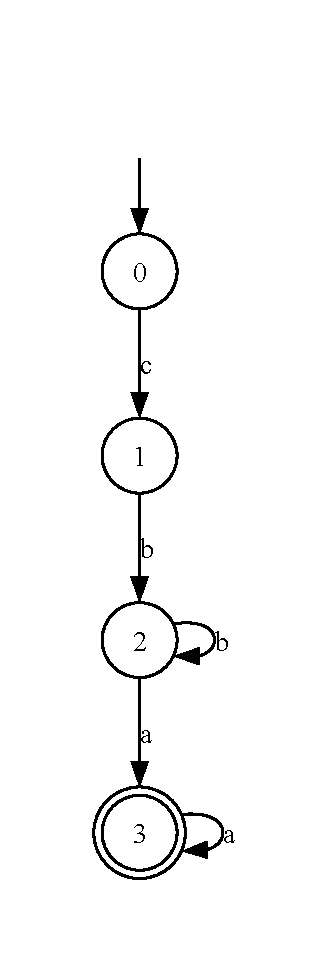
\includegraphics[keepaspectratio, scale=0.5]{reverse_regex.pdf}
%   \caption{\dfa $\aut_{cb^+a^+}$, serving as a basis for constructing $\ftEndMarker$.}
%   \label{fig:end_marker_dfa}
% \end{wrapfigure}

$\aut_{\reverse{\pi}}$ accepts $\reverse{\pi}$, but for replace operations, we need the $\ftRegexRelucAll$ to read any $x \in \Sigma^*$ and replace only the requested pattern, leaving the rest of $x$ unmodified.
Therefore, we \emph{generalize} $\aut_{\reverse{\pi}}$, producing $\aut^{\text{gen}}_{\reverse{\pi}}$, which accepts any word $x \in \Sigma^*$.
Think of $\aut^{\text{gen}}_{\reverse{\pi}}$ as the input tape of an \nft which needs to read any word on its input, and only perform a specific operation (replacement here) for a specified pattern in the input word.

Given $\aut_{\reverse{\pi}} = (\states, \Sigma, \post, \{ q_0 \}, \finalStates)$, we construct $\aut^{\text{gen}}_{\reverse{\pi}} = (\states^{\text{gen}}, \Sigma, \post^{\text{gen}}, { s_0 }, \finalStates^{\text{gen}})$ where $\states^{\text{gen}} = \{ t \,\mid\, t \subseteq \states \}$ following these rules:\newline
We define a bijective mapping $\mathcal{M}: \states^{\text{gen}} \rightarrow 2^{\states }$ such that $\forall s \in \states^{\text{gen}}, a \in \Sigma: s' \in \post^{\text{gen}}(s, a)$
iff $\mathcal{M}(s') = \{ q_0 \} \cup \{ q' \,\mid\, \exists q \in \mathcal{M}(s): q' \in \post(q, a) \}$
and $\mathcal{M}(s_0) = \{ q_0 \}$.

Intuitively, we construct a new \dfa from $\aut_{\reverse{\pi}}$ where each state $s$ maps to a set of states in $\aut_{\reverse{\pi}}$ which can be reached from $q_0$ with the same substrings of $\langof{\aut_{\reverse{\pi}}}$.
Since $\aut_{\reverse{\pi}}$ is deterministic, each substring will end in at most one state $s$.
Thus, $\aut^{\text{gen}}_{\reverse{\pi}}$ remains deterministic.

However, when we encounter state $s$ where $\finalStates \cap \mathcal{M}(s) \neq \emptyset$, we know that we have reached a state in the constructed $\aut^{\text{gen}}_{\reverse{\pi}}$ where the substring corresponding to $s$ is accepted by $\aut_{\reverse{\pi}}$.
That means that we have reached an end of an accepted word in $\aut_{\reverse{\pi}}$ which we want to mark (insert an end marker $\marker$ after this substring).
Therefore, we during the construction, we create a new final state $s_f$, and each time we encounter such a state $s$, we add a transition $\move{s}{\epsilon}{s_f}$, and redirect all transitions which would normally go from $s$ to start in $s_f$.
Thus the only outgoing transition from $s$ is the epsilon transition and we did not introduce a non-determinisctic choice of transition from $s$.
Then, all states except for states $s$ where $\finalStates \cap \mathcal{M}(s) \neq \emptyset$ are made final since we want to accept any arbitrary input.
We omit the original final states since reaching these states is a significant event in reading an arbitrary input which we need to handle separately.

$\aut^{\text{gen}}_{\reverse{\pi}}$ represents an \dfa which states how "far" into $\reverse{\pi}$ we are when reading an arbitrary input.
Each symbol either resets the \dfa (simulating manual backtracking) to some previous matched state or all the way up to $s_0$ (no even partial match was found, we start from the beginning of the pattern), or advances to the next state in the \dfa following the pattern.

Now, $\aut^{\text{gen}}_{\reverse{\pi}}$ accepts any string $x$ on its input.
During the run of $x$ on $\aut^{\text{gen}}_{\reverse{\pi}}$, each time an end of a substring $x_2$ where $x_2 \in \reverse{\pi}$ and $x = x_1 x_2 x_3$ is encountered, an epsilon transition is taken.
If we were to insert $\marker$ into $x$ each time an epsilon transition is taken, we would modify $x$ in such a way that the word would remain the same, only interspersed with $\marker$ after each end of $x_2$ (since $\aut^{\text{gen}}_{cb^+a^+}$ is deterministic, no other transition can be taken from the source state of the epsilon transition).
These $\marker$ represent the end markers we want to insert with $\ftEndMarker$.

See Figure~\ref{fig:generalized_end_marker_dfa} showing a generalized modification of \dfa $\aut_{cb^+a^+}$, $\aut^{\text{gen}}_{cb^+a^+}$.
For example, a word $cbcbba\marker a\marker a\marker bcb$ would be accepted by this automaton where the imaginery string symbol $\marker$ symbolically represents places where an epsilon transition was taken in the automaton.

% \begin{wrapfigure}{r}{0.3\textwidth}
%   \centering
%   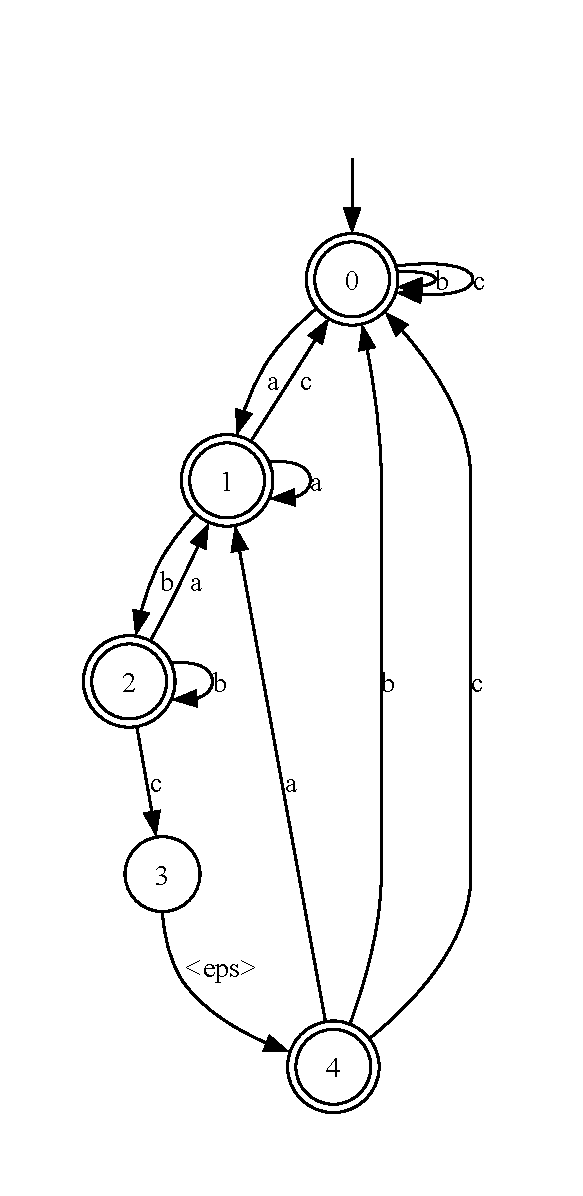
\includegraphics[keepaspectratio, scale = 0.5]{generalized_end_marker.pdf}
%   \caption{\dfa $\aut^{\text{gen}}_{cb^+a^+}$, a generalized version of $\aut_{cb^+a^+}$.}
%   \label{fig:generalized_end_marker_dfa}
% \end{wrapfigure}

Next, we can construct $\ftEndMarker$ from $\aut^{\text{gen}}_{\reverse{\pi}}$.
We simply consider the current transitions as the input tape of $\ftEndMarker$,
and we add transition symbols for output tape: for all $a \in Sigma$, the  symbol on the output tape is $a$ again, only for input symbol $\epsilon$, the output symbol is $\marker$.

We can see the final $\ftEndMarker$ for $\aut^{\text{gen}}_{cb^+a^+}$ in Figure~\ref{fig:generalized_end_marker_dft}.
% \vspace*{-1cm}
\begin{figure}[ht]
    \centering
    \subfloat[
      \dfa $\aut_{cb^+a^+}$, serving as a basis for constructing $\ftEndMarker$.
      \label{fig:end_marker_dfa}
    ]{{
      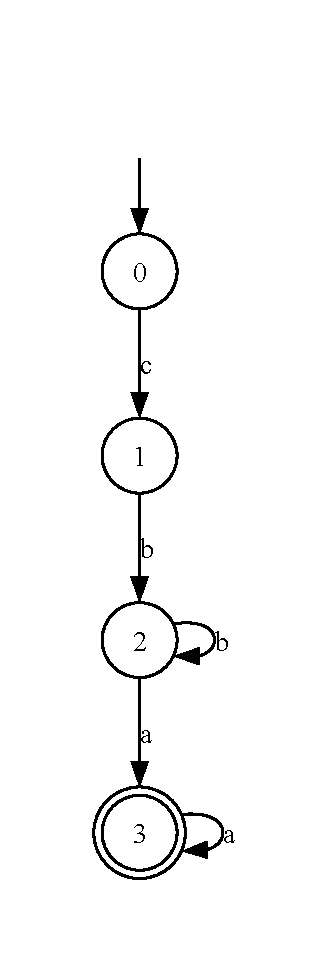
\includegraphics[keepaspectratio, width=0.2\textwidth]{reverse_regex.pdf}
    }}%
    \quad
    \subfloat[
      \dfa $\aut^{\text{gen}}_{cb^+a^+}$, a generalized version of $\aut_{cb^+a^+}$.
      \label{fig:generalized_end_marker_dfa}
    ]{{
      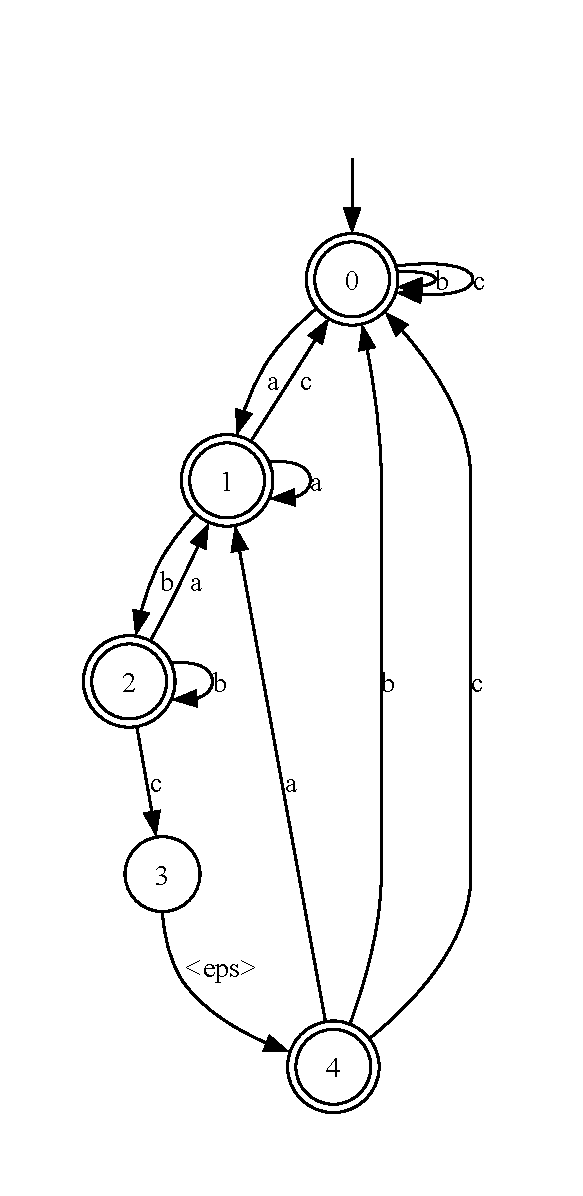
\includegraphics[keepaspectratio, width=0.33\textwidth]{generalized_end_marker.pdf}
    }}%
    \quad
    \subfloat[
      \dft $\ftEndMarker$ for $\aut^{\text{gen}}_{cb^+a^+}$ inserting the end markers $\marker$ at the correct locations in the read input word.
      \label{fig:generalized_end_marker_dft}
    ]{{
      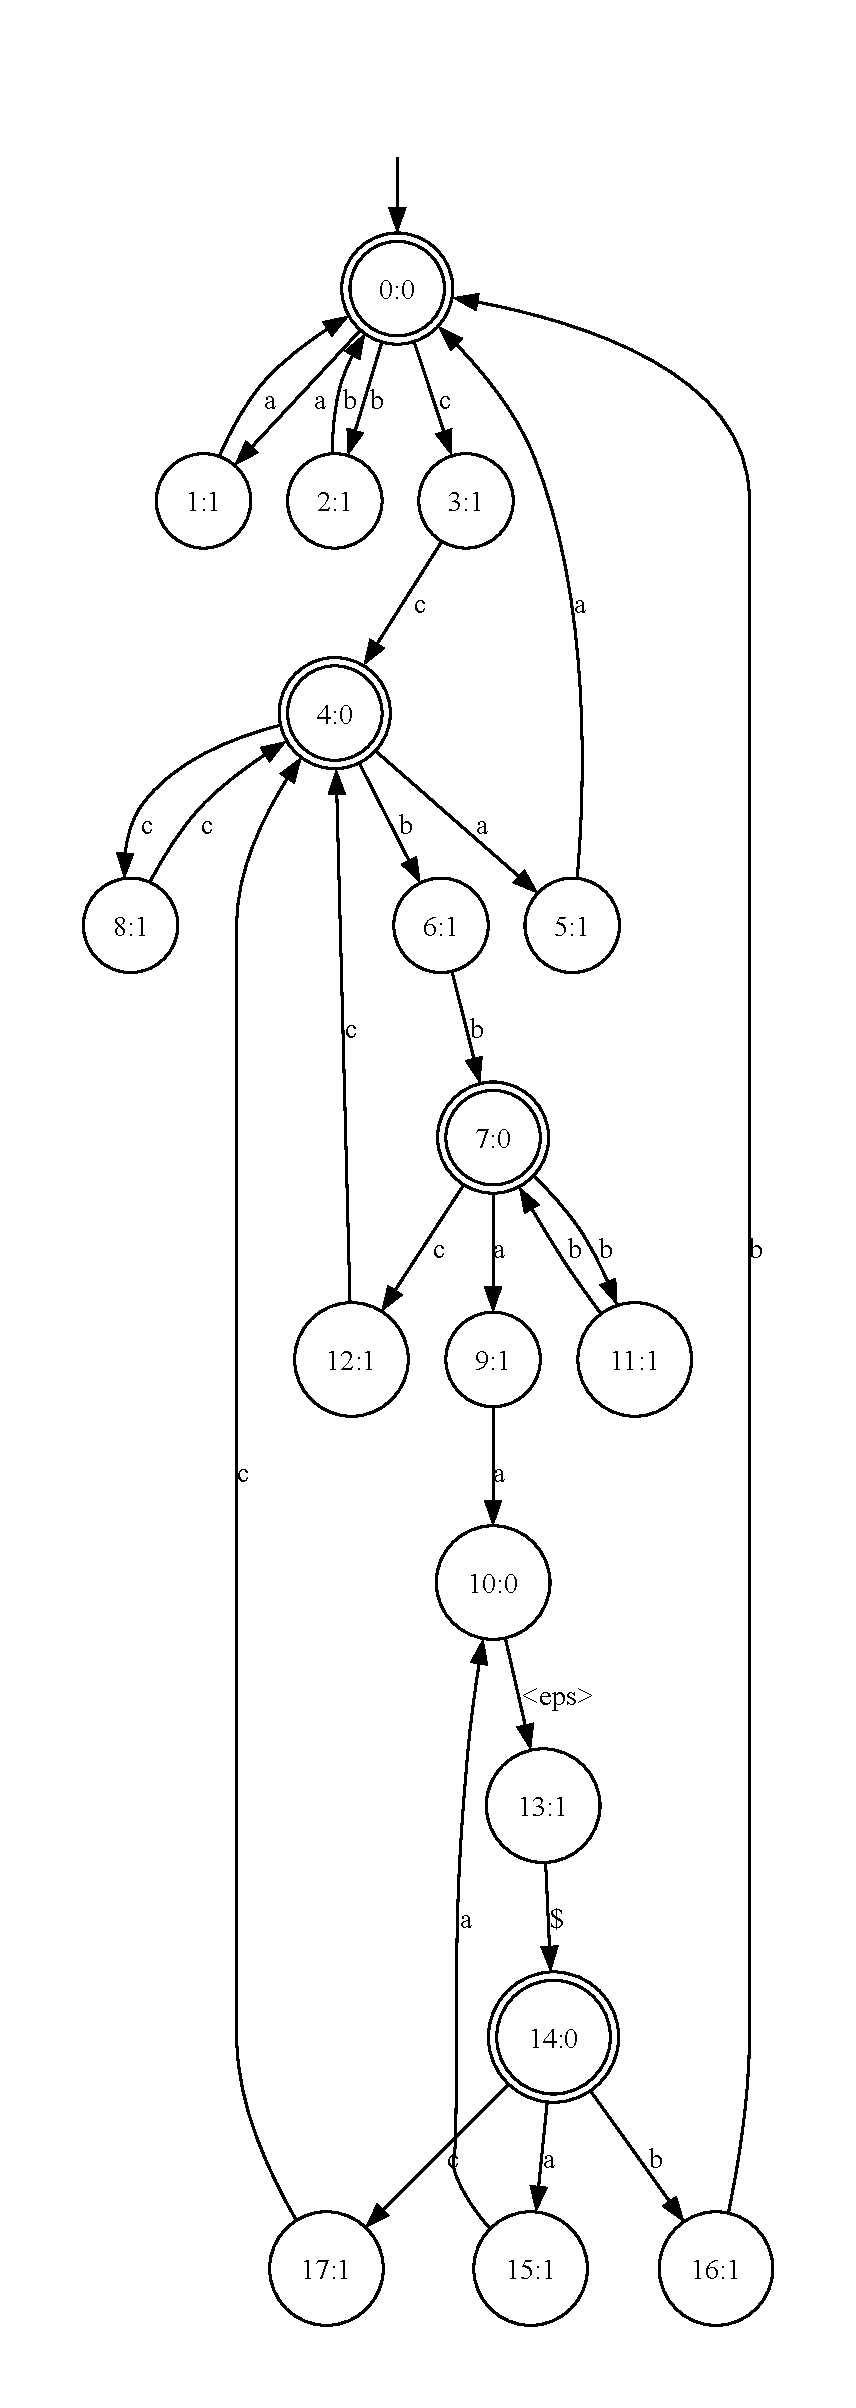
\includegraphics[keepaspectratio, width=0.33\textwidth]{end_marker_dtf.pdf}
    }}%
    \caption{
      Automata created during $\ftEndMarker$ construction.
    }
    \label{fig:end_marker_auts}%
\end{figure}

\subsection{Begin Marker \nft}

We could start constructing the \emph{begin marker} \nft $\ftBeginMarker$ from $\ftEndMarker$ by reversing all transitions in $\ftEndMarker$.
However, considering reversing a single transducer transition (consisting of operations on the input and output tapes), represented as a sequence of two \nfa transitions in \mata from state with level $0$ to $1$ and back to some state with level $0$, we instead utilize $\aut^{\text{gen}}_{\reverse{\pi}}$ before its conversion to $\ftEndMarker$ (and $\ftEndMarker$ is therefore never truly constructed in \mata).

% \vspace*{-5cm}
\begin{wrapfigure}{r}{0.3\textwidth}
  \centering
  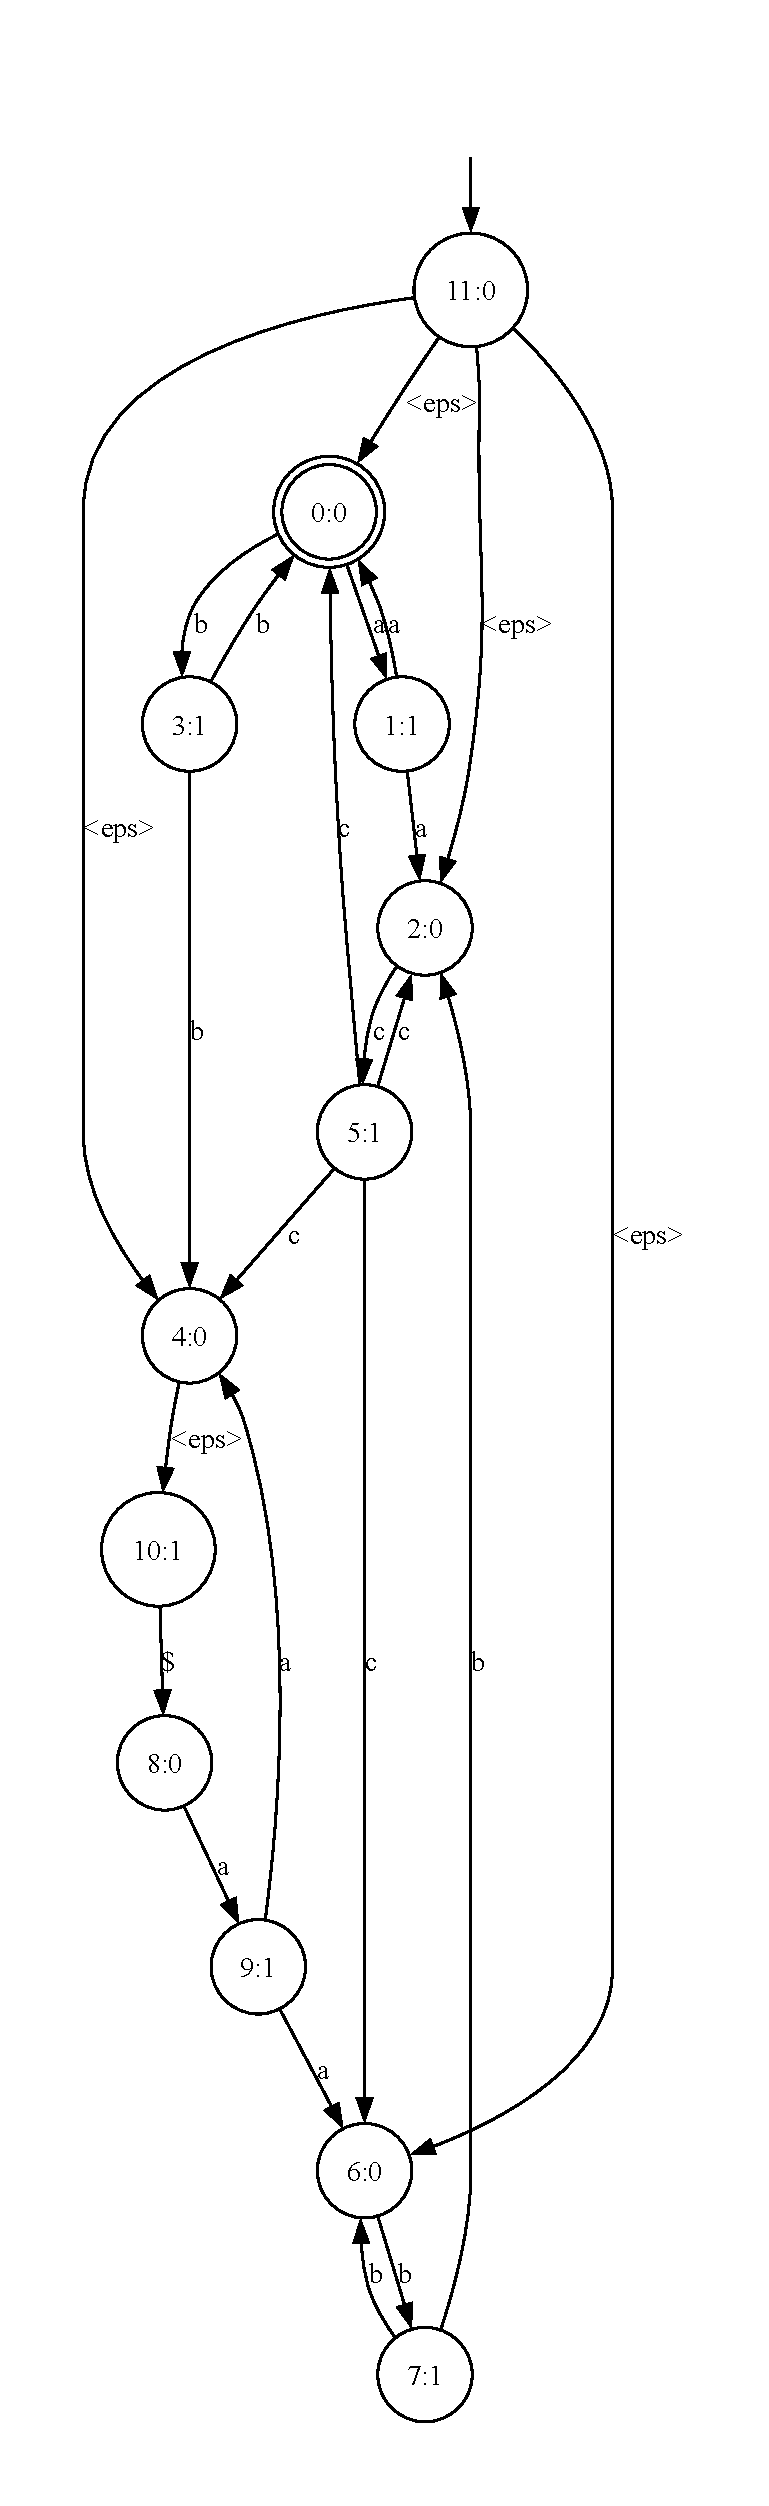
\includegraphics[keepaspectratio, scale=0.3]{nft_begin_marker.pdf}
  \caption{\nft $\ftBeginMarker$ for $\reverse{\aut^{\text{gen}}_{cb^+a^+}}$ inserting non-deterministically the begin markers $\marker$ at the beginning of matches in $a^+b^+c$ for the read input word.}
  \label{fig:begin_marker_nft}
\end{wrapfigure}

We reverse all transitions in $\aut^{\text{gen}}_{\reverse{\pi}}$, effectively obtaining the foundation for an \nfa for marking beginnings of $\pi$.
We can now construct $\ftBeginMarker$ the same way as we constructed $\ftEndMarker$ from $\aut^{\text{gen}}_{\reverse{\pi}}$ except now $\marker$ as the output symbol for the epsilon symbol on the input tape represents the begin marker instead of the end marker.
This is why we use the same marker for symbols for both the begin and end marker, as noted earlier.
They mark the same location, only once operating on $\reverse{\pi}$, then on $\pi$.

However, marking beginnings is non-deterministic operation since we cannot know in advance whether the currently read symbol in an arbitrary input string marks a beginning of a full match in $\pi$.
Henceforth, we have introduce another source of non-determinism, which gives us the smart "look-ahead" ability for marking beginnings for only those inputs that will later on truly match in $\pi$.
All potentially incorrectly inserted begin markers in the input word end in a non-accepting run for the word with such begin markers.
We add a new initial state $s'_0$ and add an epsilon transducer transition $\move{s'_0}{\epsilon}{s}$ ($\epsilon$ as the transition symbol on all tapes) leading to all states $s$ which are final in $\aut^{\text{gen}}_{\reverse{\pi}}$, that is, all except those which map to set of states containing the original final state from $\aut_{\reverse{\pi}}$.
The previous initial state of $\ftBeginMarker$ is set as the only final state and is removed from the initial states.

The Figure~\ref{fig:begin_marker_nft} shows a $\ftBeginMarker$ for $\reverse{\aut^{\text{gen}}_{cb^+a^+}}$.

\subsection{Reluctant Replacement \nft}

When we have the begin marker \nft $\ftBeginMarker$, we can construct the second \nft performing the actual replacement.
These two \nfts are used to finally construct the whole $\ftRegexRelucAll$.

We already can non-deterministically find the correct begin markers, but we now need to perform the actual replacement(s) on the input string annotated with begin markers.

We construct an \nft $\ftRegexRelucReplaceAll$ which models the actual reluctant replacement.
The idea is that we read the input string annotated with begin markers and output the same symbols unmodified on the output tape.
Once we encounter the begin marker, we know we have found the first left-most match which needs to be replaced.
Therefore, we switch to a "replacement" mode where we read the match without outputting anything, removing all symbols of the match and all additional begin markers inside the match.
Afterwards, the match is read and we can insert the replacement for the match onto the output tape.
When the replacement is inserted, we return to the beginning to potentially perform replacement on another match.

First, we convert the $\aut_{\pi}$ into a new \nfa $\aut^{\text{short}}_{\pi}$ which accepts (matches) only the shortest input words.
This can be easily performed by removing all outgoing transitions from all final states in $\aut_{\pi}$.
Clearly, $\langof{\aut^{\text{short}}_{\pi}} = \{ u \in \langof{\aut_{\pi}} \,\mid\, \neg \exists u' \in \langof{\aut_{\pi}}^{<|u|} \}$.

$\aut^{\text{short}}_{\pi}$ now matches the shortest words in the language of $\aut_{\pi}$, but does not allow skipping over additional $\marker$ encountered during the reading of the match.
Such $\marker$ need to be skipped since $\marker$ inside the shortest left-most match represent beginnings of potential matches further to the right than the left-most match.
We need to therefore add a self loop to every state in $\aut^{\text{short}}_{\pi}$ with transition symbol $\marker$.

Now the final modification is to keep the next begin marker for the next shortest left-most match. $\aut^{\text{short}'}_{\pi}$ can be constructed given $\Sigma^*_\marker = \Sigma^* \cup \{ \marker \}$ as $\aut^{\text{short}'}_{\pi} = \aut^{\text{short}}_{\pi} \cap \overline{\Sigma^*_\marker \concat \{ \marker \}}$.

$\aut^{\text{short}'}_{\pi}$ can be converted into $\ft^{\text{short}'}_{\pi}$ where the existing transitions are the input tape transitions, and the output symbols are all $\epsilon$ (\nft only reading the input word---the match---and consuming the whole match including $\marker$ inside the match).

Figure~\ref{fig:ft_regex_reluc_replace_all} symbolically shows how to construct $\ftRegexRelucReplaceAll$ for replacing all shortest left-most occurrences of regular language $\pi$ with $y$.

To replace only one occurrence (the first shortest left-most match), a variation of $\ftRegexRelucReplaceAll$, $\ftRegexRelucReplaceSingle$ can be constructed, as seen in Figure~\ref{fig:ft_regex_reluc_replace_single}.
Here we do not return to the beginning after the first replace, but move to a new state with just reads the rest of the word unmodified while removing the additional $\marker$.

% \vspace*{-1cm}
\begin{figure}[ht]
    \centering
    \subfloat[
      Symbolic representation of $\ftRegexRelucReplaceAll$ for replacing all shortest left-most occurrences of $\pi$ with $y$. All occurrences of $\pi$ are being replaced.
      \label{fig:ft_regex_reluc_replace_all}
    ]{{
      \includegraphics[keepaspectratio, width=0.45\textwidth]{{jumps_synchronization-regex_reluctant_replace_all.pdf}}
    }}%
    \quad
    \subfloat[
      Symbolic representation of $\ftRegexRelucReplaceSingle$ for replacing single shortest left-most occurrence of $\pi$ with $y$. the remaining occurrences of $\pi$ are left unmodified.
      \label{fig:ft_regex_reluc_replace_single}
    ]{{
      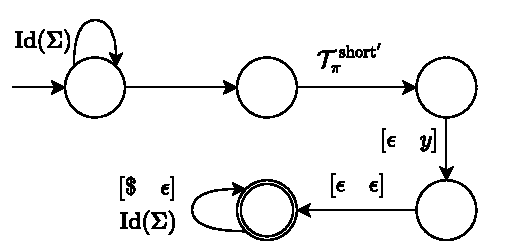
\includegraphics[keepaspectratio, width=0.45\textwidth]{jumps_synchronization-regex_reluctant_replace_single.pdf}
    }}%
    \caption{
      Symbolic representations of $\ftRegexRelucReplaceAll$ and $\ftRegexRelucReplaceSingle$.
    }
    \label{fig:regex_reluc_replace_all_single}%
\end{figure}

\subsection{Whole Regex Reluctant Replace \nft}

We have constructed $\ftBeginMarker$ to insert non-deterministically begin markers into the input word and constructed $\ftRegexRelucReplaceAll$ (or $\ftRegexRelucReplaceSingle$) to perform the replacement upon encountering matches prepended with $\marker$.
$\ftRegexRelucAll$ (and similarly $\ftRegexRelucSingle$) can be constructed by connecting these two \nfts into a sequence using composition: $\ftRegexRelucAll = \ftBeginMarker \composePipe \ftRegexRelucReplaceAll$ and $\ftRegexRelucSingle = \ftBeginMarker \composePipe \ftRegexRelucReplaceSingle$.
$\langof{\ftRegexRelucAll} = \{ (u, v) \in \Sigma^* \,\mid\, v = u^{+}_{\pi \rightarrow y} \} $ and $\langof{\ftRegexRelucSingle} = \{ (u, v) \in \Sigma^* \,\mid\, v = u^{1}_{\pi \rightarrow y} \} $.

\section{Finite Transducer for Literal Reluctant Replacement}

Constructing \nfts for regex reluctant replacement is expensive.
Therefore, when the \texttt{pattern} to be replaced is of a simpler form, namely a string literal, or even a single symbol, a corresponding \nft for reluctant replacement can be constructed faster.

\subsection{Single Symbol Replacement}

We can construct a replacement \dft for a single symbol reluctant replacement by creating a single-state \dft with $\id{\Sigma}$ self-loop transducer transitions.
Then only modify the output transition for the input symbol by replacing it with a transition (or a sequence of transitions) outputting $y$ on the output tape ($y$ can be either a single symbol or a literal) to produce the replacement.
The handling of all and single reluctant replacement variations is the same as for regex reluctant replacement: we either return to the original state, or create a new final state with $\id{\Sigma}$ self-loop transitions.

\subsection{Replacement of Finite Literal}

To construct an \nft for the replacement of a string literal $z$ with $y$, we need to construct two \nfts.

First, we want to annotate the end of the input words $x$ simlarly to how $\ftEndMarker$ annotates the end of the patterns, but now a simple \nft $\ft_\marker$ with an initial state $q_0$, final state $q_f$, and transitions $(q_0, \id{\Sigma}, q_0)$, and $(q_0, (\epsilon, \marker), q_f)$ will suffice.
$\langof{\ft_\marker} = \Sigma^* \concat \{ \marker \}$.

Second, we need to construct an \nft $\ftLiteralRelucReplaceAll$ for replacing all literals, or $\ftLiteralRelucReplaceSingle$ for replacing only the first left-most shortest literal.

$\ftLiteralRelucReplaceAll = (\states, \Gamma, \post, \{ q_0 \}, \{ q_f \})$ can be constracted using the following method.
We construct an \nft for $z$ where $z$ represents the input tape and a sequence of $\epsilon$ symbols represents the corresponding output tape.
Each state $q$ uniquely maps to its corresponding substring of $y$: $\mathcal{M}: \states \rightarrow \Sigma^*$ is a bijection where $\mathcal{M}(q_0) = \epsilon$, $\mathcal{M}(q_1) = y[0:1]$, $\mathcal{M}(q_1) = y[0:2]$, $\mathcal{M}(q_2) = y[0:3]$, etc.
Each state therefore represents a "buffer" of symbols read so far on the input tape which have not been outputted on the output tape yet.
We already have transitions as constructed from $z$ for each state.

Now we add additional transitions as follows:\newline
\begin{itemize}
  \item If $\marker$ is read on the input tape, we output the contents of the buffer $\mathcal{M}(q)$ where $q$ is the current state (symbols read from the input word but not outputted onto the output tape yet) and move to $q_f$.
  When we succeed by locating prefix starting at index $i$, we split $\mathcal{M}(q) \concat a$ into $l$ and $r$, where $l = p[0:i]$ and $r = p[i:|p|]$.
  We output $l$ onto the output tape (as a sequence of transition symbols) and move to state $q' = \mathcal{M}(r)$ which reprents the longest prefix of $y$ currently being "buffered" and not processed yet.
  \item If $a \in \Sigma, z = \mathcal{M}(q) \concat a$ ($a$ is the last symbol in $y$), we perform the replacement: outputting $y$, and move to the beginning $q_0$ to continue replacing the next matches.
  \item If $a \in \Sigma, a \neq z[|\mathcal{M}(q)|:|\mathcal{M}(q)| + 1]$ ($a$ is not the next symbol in $z$---those transitions are already in  $\ftLiteralRelucReplaceAll$), we determine the longest prefix $p$ of $z$ from $\mathcal{M}(q) \concat a$ from left to right.
\end{itemize}

When constructing $\ftLiteralRelucReplaceSingle$, instead of moving to $q_0$ after reading $z$, we move, after outputting the replacement $y$, to a final state $q_f$, and add transitions to simply read the rest of the input word and output the word unmodified onto the output tape, removing $\marker$ at the end: $(q_f, \id{\Sigma}, q_f)$ and $(q_f, (\marker, \epsilon), q_f)$.

To construct $\ftLiteralRelucAll$ (or $\ftLiteralRelucSingle$), a composition of $\ft_\marker$ and $\ftLiteralRelucReplaceAll$ (or $\ftLiteralRelucReplaceSingle$) is performed: $\ftLiteralRelucAll = \ft_\marker \composePipe \ftLiteralRelucReplaceAll$ or $\ftLiteralRelucSingle = \ft_\marker \composePipe \ftLiteralRelucReplaceSingle$.

\begin{example}
  For literal reluctant all replacement $x^{+}_{cc  \rightarrow a}$, we can see that $\mathcal{M}(0) = \epsilon$, $\mathcal{M}(1) = c$, $\mathcal{M}(2) = cc$.

  Figure~\ref{fig:literal_reluctant_replace} shows both variations (replace all and replace single) \nfts for $x^{+}_{cc \rightarrow a}$.

  Thanks to our approach, $\ftLiteralRelucAll$ and $\ftLiteralRelucSingle$ after composition maintain the same structure.
  The only difference is that marker symbols $\$$ are replaced with $\epsilon$.

\begin{figure}[ht]
    \centering
    \subfloat[
      $\ftLiteralRelucReplaceAll$ for replacement $x^{+}_{cc  \rightarrow a}$.
      \label{fig:literal_reluctant_replace_all}
    ]{{
      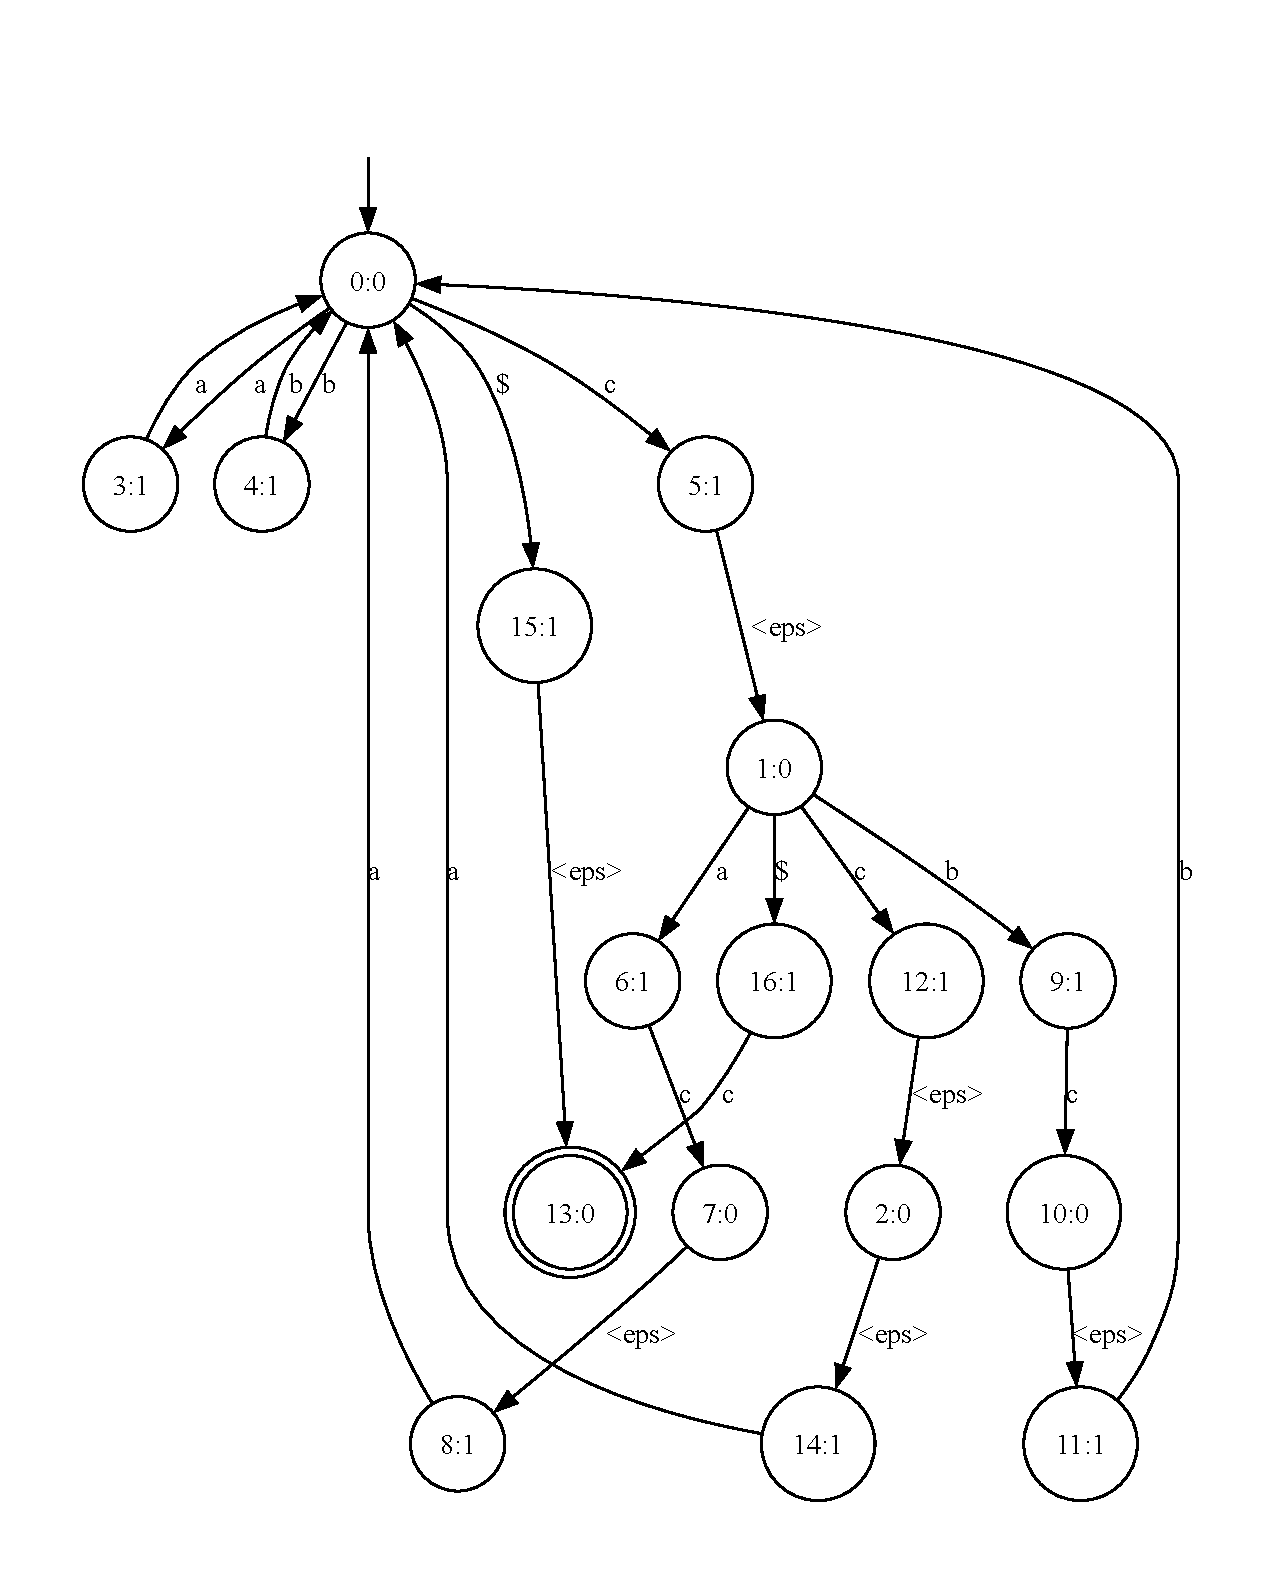
\includegraphics[keepaspectratio, width=0.50\textwidth]{reluctant_replace_literal_all.pdf}
    }}%
    \quad
    \subfloat[
      $\ftLiteralRelucReplaceSingle$ for replacement $x^{1}_{cc  \rightarrow a}$.
      \label{fig:literal_reluctant_replace_single}
    ]{{
      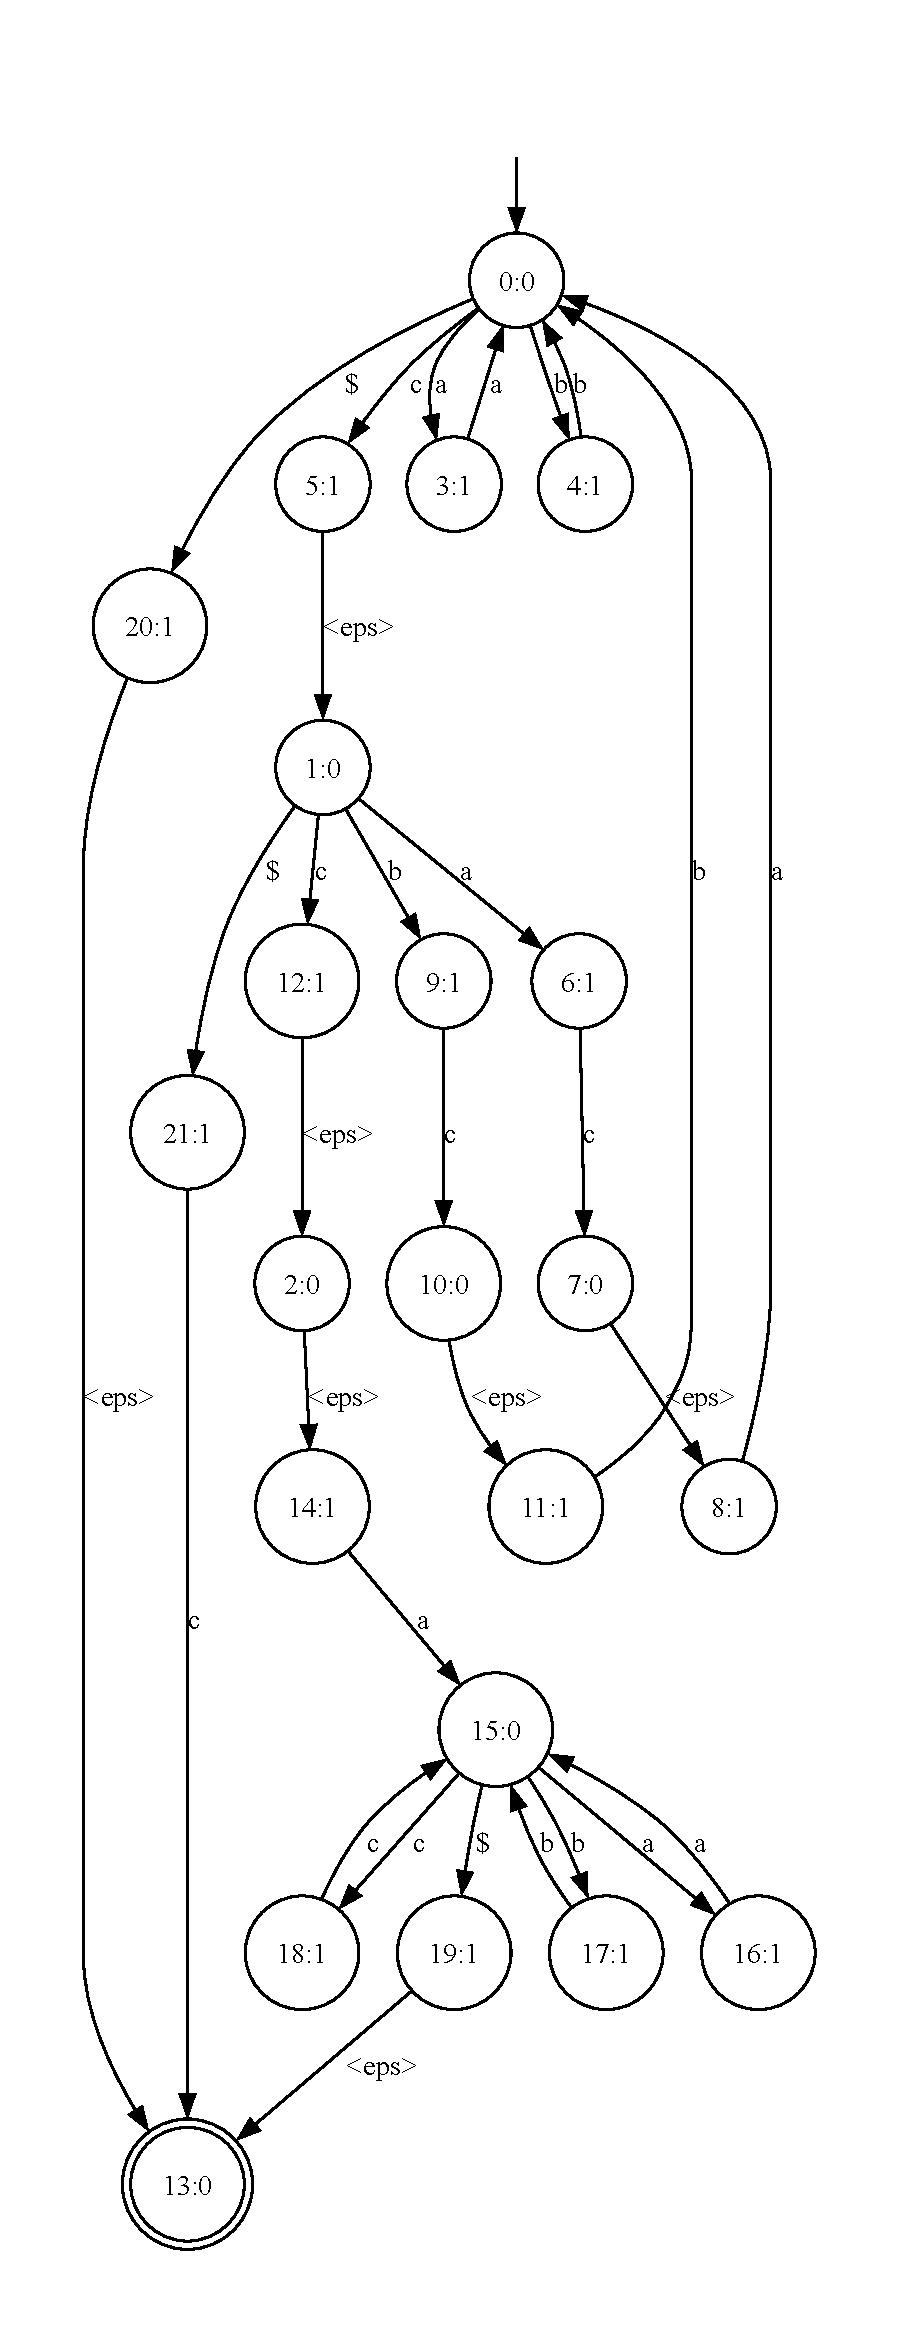
\includegraphics[keepaspectratio, width=0.33\textwidth]{reluctant_replace_literal_single.pdf}
    }}%
    \caption{
      $\ftLiteralRelucReplaceAll$ and $\ftLiteralRelucReplaceSingle$ for $x^{+}_{cc \rightarrow a}$ and $x^{1}_{cc \rightarrow a}$ replacements.
    }
    \label{fig:literal_reluctant_replace}%
\end{figure}

\end{example}

Note that this approach could be generalized to a regex replacement where the regex has finite length, similarly to how~\cite{replace_nfts_model_ModelingRegularReplacementForStringConstraintSolving_DBLP:conf/nfm/FuL10} models finite regex replacements.
However, for our uses in \noodler, we currently do not solve any industry benchmarks where finite regex replacement occurs.
Further, when modelling finite regex replacement for regex $\pi$ with the maximal length $n$ of a string $u \in \langof{\pi}$, one needs to create states for all possible substrings of $\Sigma^{\leq n}$, each with the transitions similar to those in $\ftLiteralRelucAll$.

\section{Solving SMT Formulae with Replace Operations}

The main decision procedure of \noodler rewrites SMT formulae into a form where the formula contains regular constraints (where both the variables and regular constraints have assigned regular language) and \noodler checks whether the languages for variables after restricting the languages by the string constraints are non-empty.
If during the procedure a language of some variable becomes empty, there is no assignment for the formula which could assign the variable a word satisfying the constraints.

The formulae solved by \noodler which contain replace operations always follow the following general structure:
$$ x \in \ldots \land u = \texttt{replace}(\ldots (\texttt{replace}(\texttt{replace}(x, \pi_1, y_1), \pi_2, y_2)\ldots), \pi_n, y_n) \land u \in \ldots \text{.}$$

We have a sequence of nested replace operations.
There can be between one and about 200 nested replace operations on the benchmarks from industry solved by \noodler, usually working with small tens of unique transition symbols\footnote{This is thanks to that our decision procedure in \noodler substitutes transition symbols not explicitly worked with in the formula with just two "dummy" transition symbols.}.

\begin{example}\label{ex:smt_replace_sequence}
  An encoding for operation \texttt{toUpper} which replaces all lowercase letters in $x$ with uppercase letters looks like this:
  $$ x \in \ldots \land u = \texttt{replace}(\ldots (\texttt{replace}(\texttt{replace}(x, `\text{a}`, `\text{A}`), `\text{b}`, `\text{B}`)\ldots), `\text{z}`, `\text{Z}`)\land u \in \ldots \text{.}$$.

  Another often performed operation is \texttt{HTMLEscape} which properly escapes special HTML symbols from the input string $x$ so as not to break the HTML when the user input gets inserted into the HTML webpage:
  \begin{multline*}
  x \in \ldots \land u = \texttt{replace}(\ldots (\texttt{replace}(\texttt{replace}(x, `\text{<}`, ``\text{\&lt;}``), `\text{\&}`, ``\text{\&amp;}``)\ldots), \\
  \texttt{from\_code}(39), ``\text{\&\#39;}``)\land u \in \ldots
  \end{multline*}
  where \texttt{from\_code}($n$) performs a conversion from integer code $n$ to its corresponding Unicode character.

  And finally, there are operations working with regexes $\pi$:
  $$
    x \in \ldots \land u = \texttt{replace}(x, ``\texttt{.d}^+\texttt{.}``, ``\text{\_\$1}``)\land u \in \ldots
  $$
where regex $``\texttt{.d}^+\texttt{.}``$ represents a regex descrining one or more occurrences of \texttt{d} surrounded by one character from both sides. For example \texttt{adde} matches, but \texttt{aed} does not.

All of these examples come with variants for replacing all or only the first occurence of the reex or literal, and with varying number of nested replacements.

The general approach to extend string solvers wtih support for replace operations and string transformations in general has already been pioneered in the context of monadic decomposition-based algorithms, as seen in~\cite{AnthonyReplaceAll2018, Flatten, ChainFree, StringAFA}.
However, adding this support for \noodler for its stabilization decision procedure is a challenging task with interesting impactful qualities.

\end{example}

As seen in Example~\ref{ex:smt_replace_sequence}, we often reason about regular languages for both the input and output language of the sequence of nested replace operations.
Internally in \noodler, each level of the nested hierarchy will get assigned a new fresh variable $x_i$, so we obtain from
$$
x \in \ldots \land u = \texttt{replace}(\ldots (\texttt{replace}(\texttt{replace}(x, \pi_1, y_1), \pi_2, y_2)\ldots), \pi_n, y_n) \land u \in \ldots \text{.}
$$
a formula similar to
\begin{multline*}
x \in \ldots \land u_1 = \texttt{replace}(x, \pi_1, y_1) \land u_2 = \texttt{replace}(u_1, \pi_2, y_2) \land \ldots \land \\u = \texttt{replace}(u_{n-1}, \pi_n, y_n) \land u \in \ldots \text{.}
\end{multline*}

Since we need to propagate the properties of $x$ over all the replace operations to $u$, we need a method to propagate the information over the replace operation.
Remember that now we consider both $u$ and $x$ to be string variables with an assigned regular language, $\langof{u}$ and $\langof{x}$.
The problem can be therefore split into smaller problems of form $ u = x^{+}_{\pi \rightarrow y}$ (representing a single replace operation from above) and propagating the information from $x$ to $u$.

In string solving, we work with \nfts with two tapes: the input tape and the output tape.
Thefore, we define $\projInput{\ft}$ and $\projOutput{\ft}$ as special cases of projections, performing $\projToSet{\{ 0 \}}{\ft}$ and $\projToSet{\{ 1 \}}{\ft}$, respectivelly.
Performing projection on either tape produces an \nfa representing the language of the corresponding tape.
The projection of \nft $\ft$ to its output tape, $\projOutput{\ft}$, gives us the forward image of $\ft$, \nfa $\aut_{\text{out}}$.
Similarly, the projection of \nft $\ft$ to its input tape, $\projInput{\ft}$, gives us the backward image of $\ft$, \nfa $\aut_{\text{in}}$.

For the given problem $ u = x^{+}_{\pi \rightarrow y}$ with $\aut_x$ and $\aut_u$ being the \nfas representing the regular languages assigned to variables $x$ and $u$, we can compute the language (the corresponding \nfa) of the forward image as $\projOutput{\idNft{\aut_x} \composePipe \ft_{x^+_{\pi \rightarrow y}}}$, i.e., the forward application (propagation) of $aut_x$ on $\ft_{x^+_{\pi \rightarrow y}}$ which gives us the admissible $\langof{u}$ for the given $\langof{x}$.
The backward image can be computed as $\projInput{\ft_{x^+_{\pi \rightarrow y}} \composePipe \idNft{\aut_u}}$, that is, backward application (propagation) of $\aut_u$ on $\ft_{x^+_{\pi \rightarrow y}}$ which gives us the admissible $\langof{x}$ for the given $\langof{u}$.

\paragraph{Languages of variables as concatenations of regular languages}
A decision procedure in \noodler, called \emph{stabilization}~\cite{oopsla23_stabilization_DBLP:journals/pacmpl/ChenCHHLS23}
performs automata operations on languages for variables which may be represented as a concatenation of multiple regular languages for other variables.
For an algorithm called \emph{noodlification} performed as a part of this procedure, we need to concatenate these languages with special epsilon symbols (different from those used in construction of \nfts for replace operations).
Therefore, we need to handle these symbols during replace operations as regular symbols, not epsilon symbols, in order to maintain a clear separation of languages of each individual variables in the concatenation.\footnote{The epsilon nature of these special symbols is utilized only in noodlification to indicate move between languages of variables in the concatenated language.}.

\paragraph{Flattening of the nested hierarchy of replace operations.}
To further optimize the computation of $u$ from $x$ through a nested hierarchy of replace operations, one can precompute $\ft_\text{seq}$ as a sequential composition of all \nfts for the corresponding replace operations.

Then, the hierarhcy is flattened into a single $\ft_\text{seq}$ performing all the replace operations simultanously: $u = \ft_\text{seq}(x)$.

Note that in the benchmarks solved by \noodler, the patterns being replaced are unique in that the replacement of one \nft is never later in the sequence matched to the pattern of another \nft.
E.g., operation \texttt{toUpper} performs sequence of transductions, each matching one of the lowercase letters of the alphabet and replacing it with its uppercase version.
It never happens that the uppercase letter replacing the lowercase one is later replaced with some other letter.
Therefore, an optimization of flattening a sequence of transducers satisfying this property can be utilized: the transductions in the whole sequence are associative.
We can construct intermediate \nfts for composition of any combination of \nfts in the sequence, disregarding the order of the \nfts in the sequence to more quickly construct the final \nfts for the whole sequence.
The reason for why the nested hierarchy is necessary for SMT formulae encoded in SMT-LIB format is that since the SMT-LIB format does not allow specifying a single replace operation with multiple (\texttt{pattern}, \texttt{replacement}) pairs, performing operations such as \texttt{toUpper} can be encoded only as a sequence of independent replacements which is however an unoptimal encoding for SMT solvers, especially those which can utilize the abilities of \nfts for the representation of replace operations.

\paragraph{Length constraints.}
Some variables may be length constrainted in addition to the string constraints.
Length constraints for variables are in \noodler solved separately using a LIA (linear integer arithmetic) solver provided by \ziii.
If the variables $u$ and $x$ are length variables, we need to maintain the information about lengths through the replace operation (which can in general change the length of words between $u$ and $x$).
To propagate lengths of words through the replace operations, an option would be to compute an existential Presburger formula $\phi$ based on a computation of a Parikh image of $x^{+}_{\pi \rightarrow y}$, as described in~\cite{ChainFree}.

We compute the standard Parikh image~\cite{DBLP:conf/icalp/SeidlSMH04} on the \nft for replace operation with the whole $n$-tuples of transition symbols being handled as single macrosymbols (obtaining an \nfa over the language of said $n$-tuples).
$\phi$ now encodes the relationship between the number of occurrences of $n$-tuples (macrosymbols) in $s \in \langof{\ft_{x^{+}_{\pi \rightarrow y}}}$.
To get the relationship between the actual letters $a \in \Sigma$ inside the $n$-tuples $\alpha$, we must extend $\phi$ with variables $a_i$ counting the number of occurrences of each $a$ on each tape $i$ ($i$-th element of $\alpha$), and compute the relationship between each $a_i$ and $\#\alpha$, representing the number of $\alpha$ symbols in the Parikh image, as: $a_i = \sum_{\alpha \in \Sigma^n_{\epsilon}: \alpha[i] = a} \#\alpha$ where it must hold that $|x_i| = \sum_{a \in \Sigma} a_i $ is the length of words on each tape $i$.

% TODO: What needs to be modified.
The existing decision procedure of \noodler will have to be modified further as follows:
\begin{itemize}
  \item Add saturation of replace operations, similarly to how \noodler saturates other string functions,
  \item Inclusion graph~\cite{fm23_equations_synergy_regular_constraints_DBLP:conf/fm/BlahoudekCCHHLS23} used by \noodler will have to be extended to support replace operations.
\end{itemize}

\chapter{Implementation}

The proposed data structures for finite transducers, standard operations on finite transducers, and algorithms for modelling replace operations were implemented in \mata.

The majority of the operations on finite transducers closely follow the implementation of the corresponding operations on \nfas already existing in \mata.
These operations are modified only in places where it is necessary to handle the differences between \nfas and \nfts, such as correctly setting and resetting the vector of levels for transducer states, or handling epsilon, \nop and don't care symbols.

Furthermore, several algorithms specific for \nfts are added to \mata, namely composition of two \nfts, application (of both an \nfa and a word) on an \nft, projection (to a specified subset of \nft tapes---producing a new \nft---or to only a single tape---producing the corresponding \nfa for the specified tape).

\paragraph{Levels.}
The vector of levels is a vector of unsigned integers representin the levels indexed by states.

Each \nft also stores the number of tapes (levels) in the \nft.
The number of tapes defaults to $1$, which means that the \nft is equivalent to \nfa and the operations on \nfts with number of levels set to $1$ will behave the same as a corresponding \nfa (with an equivalent transition relation where all don't care transitions are replaced with transition between the same states over the whole alphabet).

This is useful as it keeps the data structures in \mata consitent with the behaviour expected by many potential users of \mata.

\paragraph{Epsilon and no operation transitions.}
We have decided to unify the symbols for epsilon transitions and \nop transitions used in \mata.
We represent both transitions with a transition over an epsilon symbol $\epsilon$, corresponding to the largest unsigned integer value of a symbol in \mata.

To distinguish between both, we check whether the epsilon transition leads from a state with level $k$ to a state with level $k + 1 \mod n$ or not whenever we encounter the symbol in algorithms.
This operation has constant complexity since a set of levels in \mata is a state-idexable vector of levels.

We decided for this approach since all operations in \mata already support epsilon transitions, checking for existence of epsilon transitions and accessing them has constant complexity, and adding handling for yet another special transition symbol is further complicates the logic for many operations which do not have to distinguish between epsilon and no operation transitions.

\paragraph{Words and identity insertion.}
We also implemented a few utility functions which are useful when constructing or modifying \nfts\footnote{Especially for modelling the replace and other operations in string solving.} such as
\begin{itemize}
  \item \emph{inserting an identity transition} over all tapes (all tapes read/write the same symbol) over the given alphabet for a specified state.

  This is specially useful for string solving where usually one specially handles a small subset of transitions symbols, but wants to leave the remaining symbols in the input word unmodified.

  \item \emph{inserting a word} for specified tapes or \emph{inserting words}, one for each tape.

  This allows one to quickly create transducers which read a specific word, replace a specific string literal with a given literal, or removes specified literal from the input word.
\end{itemize}

\paragraph{Specifying tapes to work on.}
Since we aim to implement \nfts in \mata so they are usable for general purposes, not only limited to string solving, we allow for the majority of operations to specify what is the interpretation of each tape: e.g., which tapes are to be the input tapes, and which are to be the output tapes in application of a word or a language; or which tape(s) to use for synchronization during composition.

Be mindful that using different tapes for some operations may affect the performance of these operations. For example, application on the first tape is more performant than the application on the last tape in an $n$-tape \nft.

\section{Similarities with Operations on BDDs}

Since the idea of data structures and operations for \nfts in \mata was to provide the same underlying data structures as well as the interface for both \nfts and BDDs, many of the operations on \nfts and BDDs follow the same general algorithm with just slight modification in how \nfts and BDDs interpret the same instance of an \nft automaton.
For example, when using BDDs, one will interpret jumps over several levels to represent a sequence of transitions where the first transition has the transition symbol given by the jump, but the remaining transitions have $\dontCare$ symbols as opposed to the \nft interpretation where all transitions in the jump have the jump symbol.

As a foundation for \nft-specific operations from Section~\ref{sec:Algorithms}, we have utilized the existing implementations of intersection for BDDs.
Thanks to this, we are able to add official support for BDDs into \mata easily by inheriting \nft and modifying handling of jump transitions and several additional changes.
Therefore, \nft projection will be similar to BDD projection, \nft application is similar to BDD application, and so on.


\chapter{Experimental Evaluation}

In this chapter, we compare the performance of \nfts implemented in \mata with a state-of-the-art automata library \mona~\cite{mona}.

For our experiments, we are especially interested in how \mata performs when running operations on \nfts modelling the replace operations required by \noodler.
Since our main indent is to use \nfts in \mata as models to replace operations in \noodler, we need to optimize the \nft algorithms primarily to this use case, while keeping the \nft algorithms general enough for other use cases.

Even if \mona does not support finite transducers directly, we have chosen \mona to compare \mata against because \mona is a well-optimized library which, thanks to its ability to encode transition relation into MTBBs, provides a reasonable model for encoding finite transducers and therefore the replace operations.
Each tape in a transducer can be encoded as a single variable in the BDD for a given transition.
A sequence of variables then encodes an \nft transition, where the leaves of the BDD are target states and edges represent the transition symbols.

Performing operations such as composition, projection, or application on \nfts is, thanks to how \mata encodes \nfts as a representation very close to the representation of BDDs, a natural operation for \mona in the encoding explained above.

Intuitively, \mata performs modified \nfa operations on \nfts while \mona performs its BDD operations with the proper encoding, leading to a correct result of \nft operations in both libraries.

\paragraph{Benchmarks.}

For benchmarks, we have generated a set of benchmarks from runs of \noodler on benchmarks from SMT-LIB~\cite{SMTLIB} which contain string replace operations \texttt{str.replace}, \texttt{str.replace\_all}, \texttt{str.replace\_re} and \texttt{str.replace\_re\_all}.

We compare the performance of \mata and \mona on operations
\begin{itemize}
  \item projection to input/output tapes ($1749$ instances),
  \item application of a word on an \nft ($2027$ instances),
  \item application of a language on an \nft, and
  \item composition ($2879$ instances).
\end{itemize}

For construct an \nft for each unique replace operation in benchmarks from SMT-LIB solved by \noodler.
Furthermore, we extend this list by constructing \nfts for partial compositions of a sequence of replace operations (various subsequences) which appear in the SMT-LIB benchmarks.

All of these are the operations which will often be used on \nfts created to replace operations in \noodler and will make up the main set of operations on \nfts once support for transducers in introduced in \noodler as well.

Furthermore, these are the operations usually performed in any general use of transducers, since they comprise all the transducer-specific operations one needs when working with transducers.

\section{Results}

\subsection{Projection}

We show the performance of projection on a $2$-tape \nfts on the input tape (projecting out the output tape), and the output tape (projecting out the input tape) separately, since in $2$-tape \nfts, both cases project the first or the last tape, which is a requires a more complex modification of the \nft than projection of a tape in the middle between another tapes.

Table~\ref{tab:projection} shows comparison of performance of \mata and \mona on the projection operation on both benchmarks.

\begin{table}[ht]
  \centering
  \begin{tabular}{lrrrrrrr}
\hline
 method   &   min &     max &   mean &   q(0.25) &   median &   q(0.75) &   std. dev \\
\hline
 mata-0   &  0.07 &  285.33 &   3.20 &      1.37 &     2.66 &      3.96 &      10.43 \\
 mona-0   &  0.01 &  324.46 &   1.56 &      0.11 &     0.82 &      1.54 &      11.25 \\
 mata-1   &  0.10 & 2681.06 &  54.57 &      7.64 &    60.68 &     69.92 &      94.94 \\
 mona-1   &  0.01 &  351.74 &   1.32 &      0.08 &     0.64 &      1.22 &      11.47 \\
\hline
\end{tabular}

  \caption{
    Table comparing performance of \mata and \mona on projection on both benchmarks.
    The shown times are in milliseconds.
    The table shows the tool and which projection was performed used (tool name and the tape being projected out); and runtimes: minimal, maximal, mean, quantile 0.25, median (quantile 0.50), quantile 0.75, standard deviation.
  }
  \label{tab:projection}
\end{table}

The figures in Figure~\ref{fig:projection} show the same comparison between \mata and \mona with scatter plots: Figure~\ref{fig:projection_0} shows the projection to tape $1$ (projecting out the tape $0$) and Figure~\ref{fig:projection_1} the projection to tape $0$ (projecting out the tape $1$).

\begin{figure}[ht]
    \centering
    \subfloat[
      Scatter plots comparing the performance of \mata and \mona on projection to tape $1$ (projecting out the tape $0$).
      \label{fig:projection_0}
    ]{{
      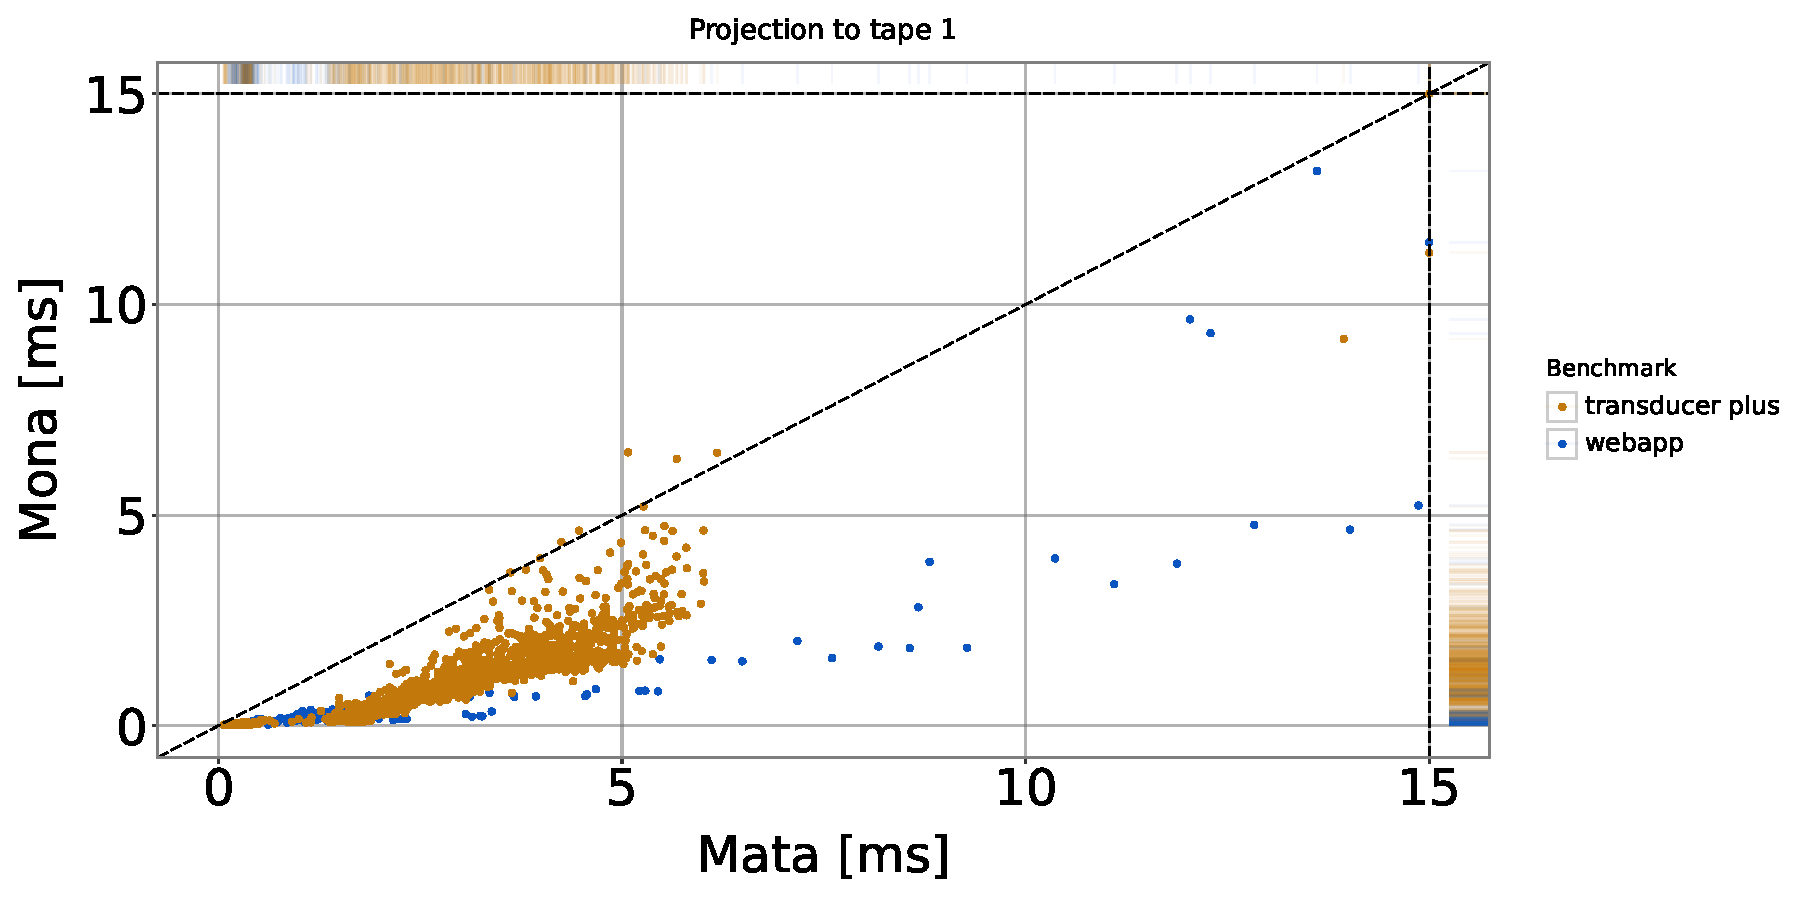
\includegraphics[keepaspectratio, width=0.45\textwidth]{projection_scatter_0.pdf}
    }}%
    \quad
    \subfloat[
      Scatter plots comparing the performance of \mata and \mona on projection to tape $0$ (projecting out the tape $1$).
      \label{fig:projection_1}
    ]{{
      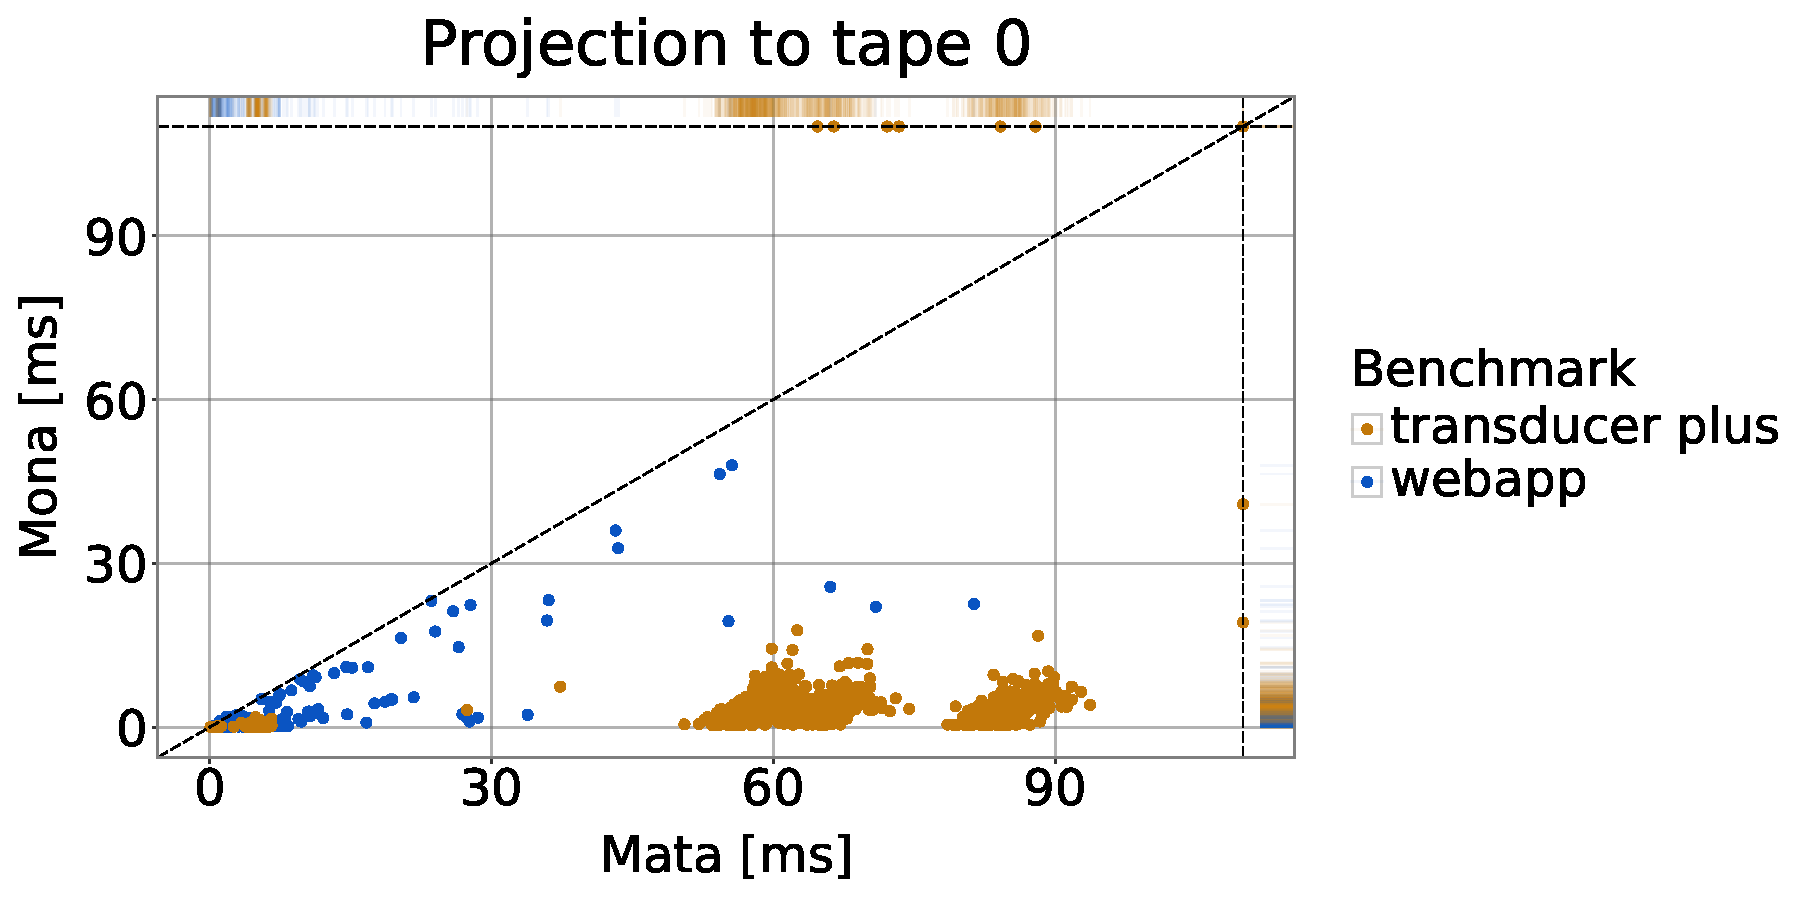
\includegraphics[keepaspectratio, width=0.45\textwidth]{projection_scatter_1.pdf}
    }}%
    \caption{
      Scatter plots comparing performance of \mata and \mona on operation projection.
    }
    \label{fig:projection}%
\end{figure}

We can see that all projections to tape $1$ finish in under $350$ ms.
By comparing means, we can see that the \mata is about 2 times slower than \mona, but is still fast, finishing $75\%$ of executions in under $4$ ms.

On the other hand, projecting to tape $0$, i.e., projecting out the tape $1$ is more expensive operation for \mata in the implemented data structure.
However, even than \mata finishes $0.75\%$ of executions in under $70$ ms.
Comparing to \mona, encoding of \nfts in \mona ensures that the projecting out the tape $1$ is similarly expensive to projecting out the tape $0$.
If the performance of \mata on projection to tape $0$ proves insufficient when support for \nfts is added in \noodler, one can omit projecting synchronization levels after every composition (and keep the synchronization levels inside the \nft), or apply the suggested specialization for composition for $2$-tape \nfts which does not need to perform projection at all.

\subsection{Application}

On each unique \nft, we applied a word and a language using \nft application.

\subsubsection{Application of a Literal}

Table~\ref{tab:language_application} shows comparison of performance of \mata and \mona on the application operation on both benchmarks applying a language $\Sigma^*$.

\begin{table}[ht]
  \centering
  \input{obrazky-figures/apply_language.tex}
  \caption{
    Table comparing performance of \mata and \mona on an operation language application on both benchmarks.
    The shown times are in milliseconds.
    The table shows the tool and which projection was performed used (tool name and the tape being projected out); and runtimes: minimal, maximal, mean, quantile 0.25, median (quantile 0.50), quantile 0.75, standard deviation.
  }
  \label{tab:language_application}
\end{table}


\subsubsection{Application of a Literal}

Table~\ref{tab:literal_application} shows comparison of performance of \mata and \mona on the application operation on both benchmarks applying a literal constructed as the longest word in the \texttt{pattern} of the replace operation constrainted to the maximal length of word $5$.

\begin{table}[ht]
  \centering
  \input{obrazky-figures/apply_literal.tex}
  \caption{
    Table comparing performance of \mata and \mona on an operation literal application on both benchmarks.
    The shown times are in milliseconds.
    The table shows the tool and which projection was performed used (tool name and the tape being projected out); and runtimes: minimal, maximal, mean, quantile 0.25, median (quantile 0.50), quantile 0.75, standard deviation.
  }
  \label{tab:literal_application}
\end{table}

\subsection{Composition}

We performed composition of various \nfts appearing in a sequence in SMT-LIB benchmarks including composition of pre-constructed partial compositions of \nfts for replace operations in these sequences.

Table~\ref{tab:composition} shows comparison of performance of \mata and \mona on the composition operation on both benchmarks.

\begin{table}[ht]
  \centering
  \input{obrazky-figures/composition.tex}
  \caption{
    Table comparing performance of \mata and \mona on an operation composition on both benchmarks.
    The shown times are in milliseconds.
    The table shows the tool and which projection was performed used (tool name and the tape being projected out); and runtimes: minimal, maximal, mean, quantile 0.25, median (quantile 0.50), quantile 0.75, standard deviation.
  }
  \label{tab:composition}
\end{table}


\chapter{Conclusion}

To summarize this thesis, we have added support for a new model for finite state machines, finite state transducers, to \mata, explained the principles behind \nfts and specifically \nfts in the context of \mata and \noodler for string solving.

We have created a new data structures derived from the existing data structures for \nfas in \mata, which fit well in the overall structure and design decision of \mata.
The introduced algorithms on \nfts are closely related to the corresponding algorithms on BDDs and maintain the two main goals of \mata: simplicity and efficiency, while keeping \mata easily extensible and understandable for a wide variety of users and applicable to both the areas of automata research and industry.

Thanks to these design decision, further extending \mata with support for handling BDDs will be effortless.

We further focussed on utilizing \nfts in string solving by adding algorithms to model string replace operations defined in SMT-LIB which will be used in \noodler for solving SMT formulae with string replace operations, previously unsolvable by \noodler.

We compared the performance of \nfts in \mata with a natural encoding of transducers in the automata library \mona.

The experiments show that \mata performs slower than \mona, but still runs reasonably fast on the general algorithms suitable for all \nft types.
The performance of \mata on $2$-tape \nfts can be further improved by applying the specialized algorithm for composition for $2$-tape \nfts, or by sometimes preventing execution of projection.

Overall, the design and implementation of \nfts in \mata is feasible, functional, performs sufficiently enough, and is widely usable, with ready-for-use support for solving SMT formulae with string replace operations in \noodler.

\paragraph{Future work.}
We continue optimizing and developing \mata and the implementation of \nfts.
In the future, we want to apply \nfts to solving string SMT formulae in \noodler.
Furthermore, depending on the performance of \nfts in \noodler, we intend to add support for symbolic representations for large alphabets using bit vectors representing sequences of bits, as used in tool \lash~cite{lash} and transition representation specific to \nfts to encode \nft operations such as identity more easily.

If the performance of composition of \nfts in \noodler proves to be a bottleneck, we can implement the optimized algorithm specialized for $2$-tape \nfts.

Since the representation of \nfts in \mata is close to BDDs, we intend to study various optimizations used for BDDs to further improve the performance of \nfts in \mata.

Finally, we intent to inherit the current structure for \nfts with the corresponding operations and add support for BDDs to \mata for future uses.


%=========================================================================

% For compilation piecewise (see projekt.tex), it is necessary to uncomment it
% \end{document}

  \else
    % Tento soubor nahraďte vlastním souborem s obsahem práce.
%=========================================================================
% Autoři: Michal Bidlo, Bohuslav Křena, Jaroslav Dytrych, Petr Veigend a Adam Herout 2019

% Pro kompilaci po částech (viz projekt.tex), nutno odkomentovat a upravit
%\documentclass[../projekt.tex]{subfiles}
%\begin{document}

\chapter{Úvod}

Tento text slouží jako ukázkový obsah šablony a současně rekapituluje nejdůležitější informace z předpisů a poskytuje další užitečné informace, které budete potřebovat pro tvorbu technické zprávy ke svojí práci. Než se šablonou budete dále pracovat, je třeba vědět, jak ji správně použít. To je stručně uvedeno v~příloze \ref{jak}.

I když některým studentům pro napsání dobré diplomové práce (bakalářská práce je také diplomová -- dostává se za ni diplom) stačí znát a dodržovat oficiální formální požadavky uvedené ve směrnicích a typografické zásady, často je výhodné před započetím psaní zjistit, jaké jsou osvědčené postupy pro psaní odborného textu a jak si práci usnadnit. Někteří vedoucí svým studentům připravili popisy osvědčených postupů, které vedly k desítkám úspěšně obhájených prací. Výběr nejzajímavějších postupů, které měli autoři této šablony k~dispozici ve chvíli její tvorby, je v níže uvedených kapitolách. Má-li Váš vedoucí svoji stránku s doporučenými postupy, tyto kapitoly můžete vynechat a řídit se pokyny svého vedoucího. Pokud takovou stránku nemá, může být přečtení níže uvedeného textu vhodnou přípravou na konzultaci o plánované struktuře a náplni textu práce.

Diplomová práce je rozsáhlé dílo a tomu odpovídá i technická zpráva. Ne každý je schopen si sednout a jednoduše ji napsat. Je třeba vědět, kde začít a jak postupovat. Jedním z možných přístupů je začít psaním klíčových slov a abstraktu, abyste si ujasnili, co je v~práci nejdůležitější. O tom pojednává kapitola \ref{abstrakt}.

Po sepsání abstraktu se lze pustit do psaní samotného textu technické zprávy. Typicky si nejprve připravíme základní strukturu práce, kterou pak budeme plnit textem. Kapitola \ref{struktura} se zabývá základními informacemi a radami pro psaní odborného textu, které Vám pomohou vyhnout se začátečnickým chybám, a stanovením nadpisů kapitol a přibližných rozsahů jednotlivých částí práce. V závěru kapitoly je pak uveden přístup, kterým si lze psaní technické zprávy značně usnadnit.

Diplomové práce v oblasti informačních technologií mají určitou typickou strukturu. Po~úvodu bude následovat kapitola či kapitoly zabývající se shrnutím současného stavu, který bude v následujících kapitolách zhodnocen a bude navrženo řešení, které bude implementováno a otestováno. V závěru pak budou výsledky vyhodnoceny a bude navržen budoucí vývoj. I když se názvy a rozsahy kapitol v různých pracích liší, vždy tam lze najít kapitoly odpovídající této struktuře. Kapitola \ref{kapitoly} se zabývá obsahy typických kapitol, které se v diplomových pracích z oblasti IT vyskytují. Většina studentů ve svojí práci pravděpodobně využije pouze určitou podmnožinu popsaných kapitol, která je pro jejich práci relevantní. Uvedené popisy a rady mohou pomoci jak s~rozhodnutím, zda danou kapitolu uvést, tak i~s~vnitřní strukturou a samotným obsahem kapitoly.

Za závěrečnou kapitolou práce vždy následuje seznam použité literatury. Citacemi, které tento seznam tvoří, a odkazy na ně se zabývá kapitola \ref{citace}. Byť to tak nezkušený student nemusí vnímat, je seznam použité literatury a odkazy na něj pro práci zcela zásadní. Hodnocení práce s literaturou a citací tvoří jednu z důležitých částí posudku oponenta a bude-li chybět jediná položka, může to vést k hodnocení stupněm F, následnému disciplinárnímu řízení za plagiátorství a k vyloučení z nedokončeného studia. Nesprávná práce se zdroji může mít i další důsledky -- v roce 2018 stála křesla dva členy české vlády. Proto prosím citacím věnujte odpovídající pozornost. 

Po dokončení textu je nutné zjistit, jaké požadavky jsou kladeny na vysokoškolskou kvalifikační práci na FIT VUT v~Brně, a dořešit případné nedostatky. Formální požadavky jsou uvedeny ve směrnicích a na webových stránkách, které jsou zmíněny v kapitole \ref{formality}. Tato kapitola obsahuje i požadované rozsahy jednotlivých typů prací a další vybrané informace z~předpisů a doporučení. V závěru kapitoly je uveden přehled nejčastějších chyb, se kterými se oponenti setkávají a kterým byste se měli vyhnout. Hodnocení formální úpravy práce je pak další z důležitých součástí posudku oponenta.

Po odstranění formálních nedostatků lze práci odevzdat. Před odevzdáním práce si můžete projít kontrolní seznam (tzv. \uv{checklist}) uvedený v příloze \ref{checklist}. Samotné odevzdání listinné i elektronické verze práce je pak popsáno v kapitole \ref{odevzdani}.

V závěrečné kapitole \ref{zaver} je pak uvedeno shrnutí toho, co se lze přečtením tohoto textu dozvědět, a to nejdůležitější, na co je třeba myslet před odevzdáním práce.


\chapter{Abstrakt}
\label{abstrakt}
Pod nadpisem Abstrakt je uvedeno shrnutí práce zabírající prostor maximálně 10 řádků. Z~dobrého abstraktu by mělo být i přes jeho malý rozsah patrné, jaký problém se řešil, jaký přístup k jeho řešení byl v práci použit a jakých výsledků bylo dosaženo. Účelem abstraktu je, aby potenciální čtenář práce již po přečtení abstraktu věděl, zda v práci najde to, co hledá \cite{fitWeb}. Zbytek této kapitoly byl převzat z blogu prof. Herouta \cite{Herout}.
\bigskip

\noindent Za prvé – na abstraktu záleží. Za druhé – není těžké ho napsat. Pojďme na to.

\subsection*{K čemu je abstrakt}
Abstrakt slouží k \bf vyhledávání\rm, společně s názvem dané vědecké práce a seznamem klíčových slov. Tyto části (snad s výjimkou názvu) nejsou přímo součástí textu a nečeká se, že někdo, kdo by zasedl ke čtení dané vědecké práce, bude číst je. To, že práci čte, znamená, že už se dostal za fázi čtení abstraktu. Abstrakt mu slouží ve chvíli, kdy se ještě rozhoduje, \bf zda vůbec \rm text číst.

Když někdo tam venku hledá odpověď na svůj problém, zadá knihovnici nebo dnes spíše vyhledávacímu serveru klíčová slova, která se jeho potíží dotýkají. Na základě shody těchto klíčových slov a klíčových slov uvedených autory dostane seznam názvů prací, které by mu mohly nabízet řešení. Dobře sestavený název práce badateli pomůže vytipovat takové texty, které by mohly mít vztah k jeho problému a mohl by se zajímat o jejich přečtení.

A tady právě přichází na scénu abstrakt. Badatel si čte abstrakt vytipovaných prací a~rozhoduje se, zda práci skutečně chce číst, nebo jestli se v tomto případě jeho filtr založený pouze na jednořádkovém nadpisu zmýlil.

V tuto chvíli obvykle ještě nemá stažené nějaké PDF s celým textem, natož aby měl v ruce vytištěný fascikl. Abstrakty jsou určeny k tomu, aby byly \bf mimo text\rm , aby ležely na serverech agregujících vědecké texty. Proto první pravidlo je, že abstrakt musí fungovat samostatně -- pokud obsahuje odkazy do literatury nebo se odvolává na text (\uv{Výkonnost metody je přehledně shrnuta na straně 51.}), nedělá badateli dobrou službu, což badatel ocení tím, že si o autoru nepomyslí nic hezkého, práci si nepřečte a autora neocituje.

\subsection*{Kdy a jak psát Abstrakt}
Může dávat smysl psát abstrakt na závěr celého psaní -- jako shrnutí a skutečné anotování sepsaného díla. Já jsem vyznavačem opačného přístupu -- abstrakt píšu na samém začátku. Když píšu vědecký článek, začínám sepsáním velkého počtu klíčových slov, jež se textu dotýkají. Bývá jich více, než potom uvedu jako ona charakteristická klíčová slova používaná k indexování. Ujasňuji si tím prostor, kde se článek pohybuje -- o čem je třeba hovořit, co je v textu podstatné, čeho se dotýká. Hned po ujasnění klíčových slov formuluji nadpis a~právě abstrakt. 

Považuji za mimořádně užitečné ujasnit si právě ony čtyři části abstraktu -- Jaký problém se řeší? Jaké řešení práce nabízí? Jaké jsou přesně výsledky? Jaký je jejich význam? Když je toto jasné, text se píše skoro sám. Pokud toto má být nejasné, jak u všech všudy je možné vůbec dát dohromady smysluplnou větu v samém textu?

\subsection*{Doporučená struktura abstraktu}
Abstrakt vědecké práce se může skládat ze čtyř částí a pak být opravdu užitečný. Každá část se bude skládat z nějakých dvou, tří vět, někdy postačí jedna.

V byznysu se vžil slovesný útvar \uv{elevator pitch} -- představení ve výtahu. Ne náhodou jeho struktura připomíná právě doporučovanou strukturu abstraktu. Opravdu, autor odborného textu má do abstraktu napsat právě to, co by říkal o své práci, kdyby na to měl nejvýše dvě minuty a nemohl použít žádných slajdů, obrázků, textu. O čem by tedy měl mluvit?

\paragraph{První část -- Jaký se řeší problém? Jaké je téma? Jaký je cíl textu?}
\begin{itemize}
  \item{Tato práce řeší.}
  \item{Cílem této práce je.}
  \item{Zaměřil jsem se na.}
\end{itemize}
Nepatří sem úvodní pohádky charakteristické pro špatný odborný sloh: \uv{Naše poslední pětiletka staví před nás nové a smělé cíle}, \uv{S rozvojem výpočetní techniky a zejména zobrazovacích zařízení je stále důležitější \ldots} Ty nepatří do dobrého textu nikam, ale do~abstraktu tím méně. Pokud dokážete vyjádřit účel svého textu v jedné větě o pár slovech, udělejte to a nepřidávejte nic navíc. Stručnější zde vždy znamená lepší.

\paragraph{Druhá část -- Jak je problém vyřešen? Cíl naplněn?}
\begin{itemize}
  \item{Zvolený problém jsem vyřešil pomocí toho a toho.}
  \item{V řešení bylo použito metody té, postupu toho a analýzy oné.}
  \item{Práce představuje algoritmus takový, který.}
  \item{Data jsem zpracovával pomocí těch a těchto nástrojů a provedl vyhodnocení takové.}
  \item{Podstatou našeho algoritmu je.}
\end{itemize}

Pokud je podstatou sepisovaného odborného textu nová metodologie (= \uv{jak něco dělat}), patří přesně sem její popis. Pokud se představované řešení skládá ze tří částí, pravděpodobně v této části abstraktu budou tři věty, z nichž každá se bude věnovat jedné části řešení. Dobrý abstrakt v této části bude upřímný a přesný -- nebude si schovávat \uv{odhalování svých tajemství} až do textu. Vágní formulace podstaty řešení v abstraktu obvykle znamená, že autoři buď neumí psát a nebo vlastně nemají o čem -- ani jedno není zrovna výzva ke stažení a čtení mnoha stran textu.

\paragraph{Třetí část -- Jaké jsou konkrétní výsledky? Jak dobře je problém vyřešen?}
\begin{itemize}
  \item{Podařilo se dosáhnout úspěšnosti 87,3\,\%.}
  \item{V práci jsme vytvořili systém, který.}
  \item{Vytvořené řešení poskytuje ty a ty možnosti.}
  \item{Provedeným výzkumem jsme zjistili, že.}
\end{itemize}

Není špatným zvykem uvést v této části konkrétní číslo -- \uv{existující metodu XY jsme zrychlili pětkrát}. Pokud přínos práce není možné shrnout do dvou nebo tří vět, někde je něco velmi špatně a celý text pravděpodobně nestojí za psaní.

\paragraph{Čtvrtá část -- Takže co? Čím je to užitečné vědě a čtenáři?}
\begin{itemize}
  \item{Přínosem této práce je.}
  \item{Hlavním zjištěním je.}
  \item{Hlavním výsledkem je.}
  \item{Na základě zjištěných údajů je možné.}
  \item{Výsledky této práce umožňují.}
\end{itemize}

Při psaní vědeckých článků já sám obvykle bojuji s podobností části třetí a čtvrté. Vskutku, obě hovoří o tom, co jsou výsledky a přínosy textu. Účelem třetí části je jmenovitě a konkrétně jmenovat dosažené výsledky, úkolem části čtvrté je interpretovat jejich význam. Asi ničemu nevadí, když tato dvě sdělení do jisté míry splynou a část třetí a čtvrtá nejen že nemají každá vlastní odstavec, ale prolínají se dokonce ve společných větách.

\paragraph{Nultá část -- O co jde? Kde jsme?}
\begin{itemize}
  \item{Práce je řešena v kontextu tom a tom.}
  \item{Nauka ta a ta se zabývá studiem toho a toho.}
  \item{Stavíme na těchto a oněch nedávných pokrocích v naší oblasti.}
\end{itemize}

Někdy je nutné na sám začátek abstraktu vložit kratičké uvedení kontextu, ve kterém se~celá záležitost vlastně odehrává. Může to být přínosné~u vskutku obskurního a esoterického oboru, který leží stranou hlavního proudu. Obvykle tato část ovšem nebývá nutná a~věty v~ní obsažené bývají prototypy ohavné, rádobyodborné vaty. Je dobrou praxí zapomenout, že se tato část v abstraktu může vyskytovat. Když někdo, kdo je odborníkem v~oboru práce, přece po přečtení abstraktu zavrtí hlavou: \uv{Vůbec nevím, o čem tady můžete psát,} pouze tehdy je vhodné vložit nějaké věty s uvedením kontextu.

\subsection*{Inovace není Ignorance}

Popisuji v tomto textu jakýsi obecný model obecné diplomky. Ještě ke všemu se na začátku zaklínám, že to je můj názor a vkus a jsem zvědavý na názory a vkusy alternativní (což jsem!). Každý diplomant (Mgr. i Bc.) přitom cítí, že jeho diplomka je speciální a výjimečná. Tudíž se nebude držet nějakého schématu, které slouží pro běžné a průměrné diplomky -- tj. pro ty ostatní. Setkávám se s dobrými důvody, proč se od výše naznačeného schématu odchýlit a každoročně některým studentům odchýlení od schématu sám doporučuji. Vskutku, každá diplomka je jedinečná a zvláštní. Kdyby ne, nemusely by se psát, stačilo by je kopírovat. Ovšem vždycky před tím, než vybočíte ze standardního a kanonického způsobu organizování odborného textu, dejte si tu práci ho poznat, pochopit a zvládnout. Způsob vědecké práce, strukturování odborného textu, nebo třeba citování pramenů, může vypadat rigidně a neohrabaně, je to ale zatím ten nejlepší způsob, který jsme jako lidstvo dokázali vymyslet. Pokud ho ovládnete, pochopíte jeho výhody a nevýhody a inovujete ho, je to v pořádku a jste vítáni. Pokud se jím odmítnete zabývat, pravděpodobně neprovedete hodnotnou inovaci, ale vytvoříte \uv{paskvil}.


\chapter{Příprava základní struktury práce} 
\label{struktura}

V této kapitole jsou nejprve uvedeny obecné zásady pro psaní odborného textu a po nich následuje detailnější popis doporučeného postupu přípravy struktury a základní osnovy práce.

Před začátkem psaní textu práce je vždy vhodné zeptat se svého vedoucího, co Vám poradí a zda nemá nějakou svoji aktuální stránku s radami a pokyny. Jeho zaměření bude pravděpodobně odpovídat zaměření Vaší práce a poradí Vám tu nejvhodnější strukturu, které byste se měli držet. Dozví-li se autoři tohoto souboru o další sbírce užitečných rad, jistě sem v budoucnu budou zařazeny.

Tento text se zaměřuje na obecná doporučení a obecnou strukturu práce, kterou je vždy potřeba  modifikovat a popřemýšlet o ní na základě konkrétního zadání \cite{Cernocky}.

\section{Užitečné rady pro psaní odborného textu}

Následující pokyny jsou dostupné též na školních webových stránkách~\cite{fitWeb}. Přehled základů typografie a tvorby dokumentů s využitím systému \LaTeX{} je uveden v~knize od~Jiřího Rybičky~\cite{Rybicka}.

Hodnocenou součástí potenciálního inženýra je mimo jiné i jazyková kvalita a čistota. Naším cílem je vytvořit jasný a~srozumitelný text. Vyjadřujeme se proto přesně, píšeme dobrou češtinou či slovenštinou (případně angličtinou) a~dobrým slohem podle obecně přijatých zvyklostí. Předpokládá se dodržování pravopisných norem zvoleného jazyka práce a dodržování odborného názvosloví. Slangové výrazy jsou nepřípustné. Při pochybnostech o~překladu či přepisu cizích pojmů využijte literatury dostupné v knihovně FIT. 

Text má upravit čtenáři cestu k~rychlému pochopení problému, předvídat jeho obtíže a~předcházet jim. Dobrý sloh předpokládá bezvadnou gramatiku, správnou interpunkci a~vhodnou volbu slov. Snažíme se, aby náš text nepůsobil příliš jednotvárně používáním malého výběru slov a~tím, že některá zvlášť oblíbená slova používáme příliš často. Pokud používáme cizích slov, je samozřejmým předpokladem, že známe jejich přesný význam. Ale i~českých slov musíme používat ve správném smyslu. Např. platí jistá pravidla při používání slova {\it zřejmě}. Je {\it zřejmé} opravdu zřejmé? A~přesvědčili jsme se, zda to, co je {\it zřejmé}, opravdu platí? Pozor bychom si měli dát i~na příliš časté používání zvratného se. Například obratu {\it dokázalo se, že \ldots{}} zásadně nepoužíváme.

Za pečlivý výběr stojí i~symbolika, kterou používáme ke {\it značení}. Máme tím na mysli volbu zkratek a~symbolů používaných například pro vyjádření typů součástek, pro označení hlavních činností programu, pro pojmenování ovládacích kláves na klávesnici, pro pojmenování proměnných v~matematických formulích a~podobně. Výstižné a~důsledné značení může čtenáři při četbě textu velmi pomoci. Je vhodné uvést seznam značení na začátku textu. Nejen ve značení, ale i~v~odkazech a~v~celkové tiskové úpravě je důležitá důslednost.

S tím souvisí i~pojem z~typografie nazývaný {\it vyznačování}. Zde máme na mysli způsob sazby textu pro jeho zvýraznění. Pro zvolené značení by měl být zvolen i~způsob vyznačování v~textu. Tak například klávesy mohou být umístěny do obdélníčku, identifikátory ze~zdrojového textu mohou být vypisovány {\tt písmem typu psací stroj} a~podobně.

Uvádíme-li některá fakta, neskrýváme jejich původ a~náš vztah k~nim. Když něco tvrdíme, vždycky výslovně uvedeme, co z~toho bylo dokázáno, co bude dokázáno v~našem textu a~co přebíráme z~literatury s~uvedením odkazu na příslušný zdroj. V~tomto směru nenecháváme čtenáře nikdy na pochybách, zda jde o~myšlenku naši nebo převzatou z~literatury.

Abychom mohli napsat odborný text jasně a~srozumitelně, musíme splnit několik základních předpokladů:
\begin{itemize}
\item Musíme mít co říci,
\item musíme vědět, komu to chceme říci,
\item musíme si dokonale promyslet obsah,
\item musíme psát strukturovaně. 
\end{itemize}

\subsection*{Musíme mít co říci}
Nejdůležitějším předpokladem dobrého odborného textu je myšlenka. Je-li myšlenka dost závažná, tak přetrvá, i když je neobratně a zmateně podaná. Chceme-li však myšlenku podat co nejvýstižněji a ušetřit tak čtenáři čas, musíme dodržet určité zásady, o kterých pojednáme dále.

\subsection*{Musíme vědět, komu to chceme říci}
Dalším důležitým předpokladem dobrého psaní je psát pro někoho. Píšeme-li si poznámky sami pro sebe, píšeme je jinak než výzkumnou zprávu, článek, diplomovou práci, knihu nebo dopis. Podle předpokládaného čtenáře se rozhodneme pro způsob psaní, rozsah informace a~míru detailů.

\subsection*{Musíme si dokonale promyslet obsah}
Musíme si dokonale promyslet a~sestavit obsah sdělení a~vytvořit pořadí, v~jakém chceme čtenáři své myšlenky prezentovat. 
Jakmile víme, co chceme říci a~komu, musíme si rozvrhnout látku. Ideální je takové rozvržení, které tvoří logicky přesný a~psychologicky stravitelný celek, ve kterém je pro všechno místo a~jehož jednotlivé části do sebe přesně zapadají. Jsou jasné všechny souvislosti a~je zřejmé, co kam patří.

Abychom tohoto cíle dosáhli, musíme pečlivě organizovat látku. Rozhodneme, co budou hlavní kapitoly, co podkapitoly a~jaké jsou mezi nimi vztahy. Diagramem takové organizace je graf, který je velmi podobný stromu, ale ne řetězci. Při organizaci látky je stejně důležitá otázka, co do osnovy zahrnout, jako otázka, co z~ní vypustit. Příliš mnoho podrobností může čtenáře právě tak odradit jako žádné detaily.

Výsledkem této etapy je osnova textu, kterou tvoří sled hlavních myšlenek a~mezi ně zařazené detaily.

\subsection*{Musíme psát strukturovaně} 
Musíme začít psát strukturovaně a~současně pracujeme na co nejsrozumitelnější formě, včetně dobrého slohu a~dokonalého značení. 
Máme-li tedy myšlenku, představu o~budoucím čtenáři, cíl a~osnovu textu, můžeme začít psát. Při psaní prvního konceptu se snažíme zaznamenat všechny své myšlenky a~názory vztahující se k~jednotlivým kapitolám a~podkapitolám. Každou myšlenku musíme vysvětlit, popsat a~prokázat. Hlavní myšlenku má vždy vyjadřovat hlavní věta a~nikoliv věta vedlejší.

I k~procesu psaní textu přistupujeme strukturovaně. Současně s~tím, jak si ujasňujeme strukturu písemné práce, vytváříme kostru textu, kterou postupně doplňujeme. Využíváme ty prostředky DTP\footnote{Desktop publishing (DTP) -- tvorba tištěného dokumentu na počítači.} programu, které podporují strukturovanou stavbu textu (předdefinované styly pro nadpisy a~bloky textu).

\subsection*{Nikdy to nebude naprosto dokonalé}
Když jsme už napsali vše, o~čem jsme přemýšleli, uděláme si den nebo dva dny volna a~pak si přečteme sami rukopis znovu. Uděláme ještě poslední úpravy a~skončíme. Jsme si vědomi toho, že vždy zůstane něco nedokončeno, vždy existuje lepší způsob, jak něco vysvětlit, ale každá etapa úprav musí být konečná.

\section{Komu se píše diplomka}
Tato podkapitola byla převzata z blogu prof. Herouta \cite{Herout}.

\bigskip
\noindent \bf Pište svou diplomku pro studenta, který má na Vaše dílo navázat. \rm
\bigskip

Představte si, že na Vaší práci bude dál pracovat student Franta, asi tak stejně chytrý jako Vy sami. Máte teď čtyři hodiny na to, abyste mu svou práci ukázali, zasvětili ho do~všeho, co je potřeba, a on pak bude pokračovat sám. Franta je studentem stejné školy jako Vy a~ví asi tolik, co průměrný student, není žádným super odborníkem na obor Vaší diplomky, ale rozhodně není hloupý a řešeného tématu se neštítí. Franta, tak jako Vy, se~o~tom, že bude po Vás pokračovat, zrovna dozvěděl, takže ještě neměl čas si něco k~tématu nastudovat.

Bude dobré začít tím, že se Franta dozví, co je cílem práce, proč se to celé dělá, co mají být výsledky.

Nikdo soudný by hodinu z vyměřeného času s Frantou nestrávil řečněním typu: \uv{\mbox{Internet} byl vytvořen americkou armádou v roce 1962, pak v roce 1991 v CERNu udělali www, a~nyní se používá v nejrůznějších oblastech lidské činnosti.} (to vše na šesti stranách s~mnoha odkazy a obrázky).
Franta obvykle nepotřebuje několikastránkové skriptum o detailech barevných modelů pro reprezentaci obrázků, historii a detaily Houghovy transformace, kompletní popis vrstev referenčního modelu ISO/OSI, ani řadu koláčových grafů o~zastoupení jednotlivých mobilních platforem na trhu za posledních deset let.
Franta potřebuje nasměrovat na~cenné zdroje, které Vám při řešení pomohly, a chce letmý popis nástrojů a~algoritmů, které byly nutné pro řešení: \uv{Je potřeba nástroj XY, který slouží k tomuhle a~tamtomu, hlavně jeho modul PQ, který se používá tehdy a~tehdy. Nejlepší je k tomu tato dokumentace.}

Řekněte Frantovi hodně o tom, co se při řešení osvědčilo a co pomáhalo, ale upozorněte ho i na to, co nejdřív vypadalo jako dobrý nápad, ale pak se ukázalo jako zbytečné nebo nefunkční.

Dobře dávkujte úroveň detailu. Nějakou optimalizační fintu rozeberete ve zdrojovém kódu řádek po řádku, nějaký pomocný modul přejdete jedním odstavcem s popisem vstupů a výstupů a odkazem na použitou knihovnu.

Představte si průběh toho čtyřhodinového sezení s Frantou.
\begin{itemize}
  \item{O čem byste asi mluvili na začátku, kdy se Franta teprve začíná orientovat?}
  \item{Co jsou věci, které by rozhodně měly zaznít?}
  \item{Jaké obrázky byste v průběhu sezení malovali?}
  \item{Na co by se Franta vyptával, protože je to důležité a přitom to není samozřejmé?}
  \item{Na jaká omezení a nedodělanosti byste Frantu potřebovali upozornit, aby neupadl do~nějaké pasti?}
  \item{Jak vlastně Franta může pokračovat? Co jsou otevřené záležitosti, které by ještě stálo za to vyzkoušet a vylepšit?}
  \item{Co byste říkali úplně první (úvod) a úplně poslední (závěr) minutu sezení?}
\end{itemize}


\section{Struktura diplomové práce -- Pět kapitol}
Není-li dále uvedeno jinak, tato podkapitola byla převzata z blogu prof. Herouta \cite{Herout} (částečně inspirovaného knihou, kterou napsal Jean-Luc Lebrun \cite{Lebrun2011}) a z dokumentu na osobní stránce prof. Zemčíka~\cite{Zemcik}.
\bigskip

Diplomová práce je činnost, kterou student vyvíjí po dva semestry studia a pak o ní sepíše knížečku. Rozšířená terminologická chyba je, že se té knížečce, která je o činnosti sepsaná, říká diplomová práce. Ta knížečka je ve skutečnosti technická zpráva o provedené roční činnosti a diplomová práce je ta roční činnost.

Diplomantova roční činnost zahrnuje za prvé studium: \uv{Co už v oblasti mého zadání existuje? Jak to dělají jiní?} V rámci diplomky člověk dále nějaké věci vymyslí a navrhne: \uv{Zadaný problém lze řešit tak a nebo tak, já k němu přistoupím tímto způsobem, protože na~zvolené platformě je to nejefektivnější.} To, co řešitel navrhl, by měl po sobě ověřit tím, že to implementuje a vyhodnotí: \uv{Pro implementaci jsem zvolil ty a ty nástroje, celý systém rozvrhl do takových modulů. Výsledek je takhle rychlý, má takovou úspěšnost a~reakce uživatelů jsou takové a takové.}

Základní struktura diplomové práce podle prof. Herouta tedy je:
\begin{enumerate}
  \item{Úvod (1 strana)}
  \item{Co bylo třeba vystudovat (vč. zhodnocení současného stavu; 40\,\% rozsahu)}
  \item{Nové myšlenky, které tato práce přináší (30\,\%)}
  \item{Implementace a vyhodnocení (30\,\%)}
  \item{Závěr (1 strana)}
\end{enumerate}

Není chybou, když text má právě 5 takových kapitol, není ani chybou, když je některá z~nich rozdělena na dvě části -- o tom dále. Obvykle je velkou chybou, když tam některá část chybí, nebo má nápadně odchylný rozsah. Názvy kapitol nemusí kopírovat tuto strukturu. Samozřejmě, samotný obsah práce je nadřazen všem zásadám a pokud tedy bude dobrý důvod strukturu porušit, tak to udělejte.

Na této základní struktuře se řada vedoucích shoduje, byť různí vedoucí doporučují rozdílné názvy kapitol a např. zhodnocení současného stavu lze umístit nejen do 2., ale i~do~3. kapitoly jak to doporučuje prof. Zemčík:
\begin{enumerate}
  \item{Úvod (1--2 strany)}
  \item{Shrnutí dosavadního stavu (40--50\,\% celkového rozsahu)}
  \item{Zhodnocení současného stavu a návrh řešení (3--5 stran)}
  \item{Popis vlastní práce (cca 40\,\% celkového rozsahu)}
  \item{Závěr (max. 1 strana)}
\end{enumerate}

Názory vedoucích se dle zaměření práce liší i v rozsazích, jak je vidět např. v~doporučeních dr. Berana \cite{Beran}:
\begin{enumerate}
  \item{Úvod (1 stránka)}
  \item{Teorie (1/3 stran)}
  \item{Návrh řešení (1/3 stran)}
  \item{Realizace, experimenty a vyhodnocení (1/3 stran)}
  \item{Závěr (1 stránka)}
\end{enumerate}

U prakticky zaměřených prací, pro která jsou zásadní data a uživatelská rozhraní, lze využít doporučení od doc. Černockého \cite{Cernocky}:
\begin{enumerate}
  \item{Úvod (jednotky stran)}
  \item{Teoretická část (cca 10 stran)}
  \item{Data (jednotky stránek)}
  \item{Popis Vašeho algoritmu a jeho testování (cca 10 stran)}
  \item{Návrh a implementace (pár stran)}
  \item{Uživatelské rozhraní (pár stran)}
  \item{Testování (cca 10 stran)}
  \item{Závěr (jednotky stran)}
\end{enumerate}

\section{Diplomka -- komiksová edice}
Tato podkapitola byla převzata z blogu prof. Herouta \cite{Herout}.

Diplomka (bakalářka je taky diplomka) je poměrně komplexní dílo. Skládá se z velkého počtu písmenek. A ta písmenka nejsou jen tak za sebou, ale jsou uspořádána hierarchicky do~kapitol. Celé to musí mít nějakou logiku, nějaký sled -- čtenář se musí nejdřív dozvědět jedny věci, aby mu pak šlo přesvědčivě předat věci jiné. Musí tam být obrázky, tabulky, vzorce; zároveň si tyto ne-textové věci musí s okolním textem povídat a navzájem se doplňovat. Musí se zcela pokrýt oficiální zadání, a vše musí být doručeno k nějakému přesnému datu, vytištěné a svázané. Pokud, nad to všechno, má být diplomka dobrá, musí to všechno být uděláno dobře. Když se peče koláč z deseti surovin a jedna z nich je zkažená, celý koláč bude hnusný. Musí klapnout všechno.

\subsection*{Jak to všechno pohlídat? Odkud zaútočit?}
Když s kolegy píšeme článek (poslední dobou asi tak pořád), v hodně rané fázi připravíme něco, čemu říkáme \uv{Comics Edition}. Děláme to jednak proto, že já na tom trvám, a dvak proto, že nám to dosti pomáhá. Třeba to pomůže i Vám s diplomkou.

Nejprve si ujasněte odpovědi na následující otázky:
\begin{itemize}
  \item{Jak byste vystihli podstatu svého řešení ve třech až pěti krátkých větách?}
  \item{Jaké jsou silné stránky Vašeho řešení?}
  \item{Jaké jsou konkrétní argumenty, že to, co jste udělali, je dobré?}
  \item{Kdyby chtěl někdo být na Vaši práci zlý -- co by vytkl?}
  \item{Co byste mu odpověděli?}
  \item{Jaká klíčová slova by měl člověk zadat do vyhledávače, aby Vaše diplomka byla relevantní odpovědí?}
\end{itemize}

Pokud máte, můžeme jít na věc \ldots

\subsection*{Hned založit TEN dokument}
Občas vídám postup, že někdo píše \uv{předběžnou} verzi diplomky do nějakého poznámkovadla. Je to za prvé práce navíc a za druhé zbytečná. Je třeba hned založit dokument, ve~kterém svůj boj dokončíte, a ze kterého výsledek vytisknete.

\subsection*{Nadpisy kapitol}
Důležitou součástí komixového vydání, o něž se tu snažíme, jsou nadpisy kapitol. Vložte je do dokumentu. Vložte je tak, jak budou z hlediska formátování -- žádné provizorní seznamy: \uv{Já to pak předělám}. Chcete vidět, jak přesně to bude vypadat, jak se vyloupne celý automaticky sestavený obsah. Vložte je jak budou z hlediska jejich znění. Nadpis kapitoly říká, co v kapitole bude. Nadpisy kapitol tvoří kostru celého díla, již pak obalujete masem a kůží textu a obrázků.

Ze všech slov, která jsou v diplomce, jsou slova v nadpisech \textbf{ta nejdůležitější}. Věnujte jim opravdu mimořádnou pozornost.

\subsection*{Obrázky}
Obrázek vydá za tisíc slov. Prošel jsem 8 posledních článků, jež jsem spoluautoroval. Dohromady mají 80 stran, obsahují 87 obrázků a 17 tabulek, tj. 1,3 vizuálního sdělení na~stránku (včetně stránek obsahujících reference do literatury, úvodních stránek s abstrakty a vůbec všeho). Mnohé obrázky (tak půlka) se ve skutečnosti skládají z několika podobrázků, zvlášť odkazovaných. Těch jsem v řečených 8 článcích napočítal 221, tj. v průměru 3 vizuály na~stranu. Taková je moje představa o roli obrázků v odborném textu. Nemyslím si, že by mohla existovat vážně míněná diplomka, která by měla \uv{příliš mnoho obrázků}.

Již v rané verzi komixového vydání diplomky hleďte promyslet, kde se obrázky budou vyskytovat a jaké. Obrázky ještě nemusíte mít hotové. Zdaleka. Ještě nevíme, co přesně na~obrázku bude. Ještě nevíme, jaký pod ním bude popisek. Co víme je, že tu nějaký takový obrázek bude a že se bude skládat z více podobrázků a tak ho hned vložíme. Zabere to tak minutu (vektorovou podobu \uv{TODO Image} máme už dávno uloženou a je součástí této šablony) a hned se víc rýsuje, jak text bude vypadat. 
U některých obrázků už dokonce máme představu, jak budou vypadat -- konceptuálně. Nakreslíme na papír nebo na tabuli, vyfotíme mobilem, obrázek vložíme, aby držel místo tomu, jenž přijde po něm a bude nakreslený pořádně (vektorově v Inkscape\footnote{\url{https://inkscape.org}} nebo vygenerovaný Gnuplotem\footnote{\url{http://www.gnuplot.info/}}).

Jen tak na okraj: Obrázek vydá za tisíc slov. Hloupý obrázek vydá za tisíc hloupých slov. A když už jsme u těch obrázků: Kdo vkládá věci, které by měly být vektorové (schémata, grafy, nákresy, diagramy, prakticky všechno kromě fotek a~snímků obrazovek), jako rastrové obrázky, a kdo vkládá snímky obrazovek (a podobné věci, které mají být přesně) se ztrátovou kompresí (obvykle JPEG), nemůže očekávat pozitivní hodnocení práce.

\subsection*{Objem textu}
Zrovna tak jako vkládáme obrázky, které ještě nemáme, vkládáme i text, který ještě nemáme. V \LaTeX{}u je na to krásný příkaz \texttt{\textbackslash Blindtext}\footnote{Stručný tutorial: \url{https://texblog.org/2011/02/26/generating-dummy-textblindtext-with-latex-for-testing/}}. Kdo ho (ke své škodě) nechce nebo neumí používat, použije \url{http://lipsum.com}. Pomůže pisateli tušit přibližný rozsah celého díla, hustotu obrázků v textu a další charakteristiky textu při pohledu shůry. Vytvořit si takový odhad trvá třeba 5 minut. Pro orientaci v rozdělaném textu je rozumné tento nijaký text vybarvit šedou barvou (inteligent si na to udělá příkaz, ať se pak barva snadno jednotně změní pro celý dokument). Zkušenost říká, že bez barev v tom člověk začne mít slušný nepořádek -- co už je hotové, co ne, na čem je potřeba pracovat. Je radno investovat pár minut do zprovoznění balíčku pro barvení textu. V rámci této šablony můžete použít příkaz \verb|\todo|, např. \todo{Toto je třeba dokončit}. 

Geneze každé kapitoly ať začíná tím, že obsahuje třeba 3-5 kusů TODO a nějaké to Lorem ipsum. Každé TODO se pak postupně transformuje na větší počet TODO menšího rozsahu, nebo na text, na obrázek, další podkapitoly, cokoliv. TODO střídavě přibývají a~ubývají, práce se přitom vždycky o kousek pohne.

\subsection*{Jak s tím celým pracovat}
Když na to člověk sedne a \LaTeX{} zrovna nemá špatný den, za hodinu je hotová diplomka (bakalářka je taky diplomka) o správném počtu stran, obsahující představu, co kde bude. Začíná se podobat výsledku, který má přijít až za nějakou dobu, po nějaké práci.

Dokument pak už v zásadě nenarůstá, ale transformuje se. Je velký rozdíl sednout si před prázdnou bílou obrazovku a \uv{psát diplomku} a vzít si jedno TODO a napsat místo něj odstavec. To první je těžké a někdy to prostě nejde. To druhé jde: má to svůj začátek a konec. Ví se, co se má udělat.

Pořád platí, že diplomka se nenapíše sama, ale jde to lépe a výsledek má spíše hlavu a~patu.

\section{Jak pojmenovat kapitoly}
Dobře publikovat neznamená jen posypávat co nejvíc papíru co nejvíce písmenky. Renomé vědce vzniká vlastně až tím, že jinému vědci je jeho práce natolik užitečná, že ho cituje ve~své práci. Proto je potřeba, aby svůj článek napsal dobře: nikdo nebude citovat práci, která je humpolácky napsaná, protože by se sám shodil. 
Humpolácky napsaný článek ovšem nikdo nebude citovat už z toho důvodu, že \bf ho nenajde\rm . Už dávno před nějakým internetovým SEO vědci používali při psaní různé \uv{fligny} tak, aby je další vědec, když dělá svoji rešerši, zařadil mezi svůj materiál, jejž přečte, z něhož si nadělá poznámky a který -- nakonec a~logicky -- ocituje ve svém díle.

Na světě je moře článků. Když vědec Tonda hledá materiál relevantní pro svou práci, zadá klíčová slova (kdysi papírově do knihovny, nyní elektronicky do příslušného vyhledávače) a vypadne mu hromada nálezů -- tj. názvů. První krok, aby článek někdo ocitoval, je mít dobrý název. Tak dobrý, aby Tondu zaujal a on si název rozkliknul ve snaze zjistit více. Název je \bf prvním filtrem\rm . 

Články, jež prošly prvním filtrem, si Tonda rozklikne. To znamená, že vidí abstrakt článku. Abstrakt je \bf druhým filtrem \rm a hodně na něm záleží. Je to jako dostat se do~druhého kola pohovoru k vysněné práci. 

Když tedy Tondu zaujme nadpis i abstrakt, stáhne si celé PDF článku a rychle ho proskroluje, aby si udělal představu: vytiskne ho, nebo okno s článkem zavře a bude se věnovat desítkám jiných? To je \bf třetí filtr \rm a je to jako být mezi pár posledními uchazeči o~práci snů. Na co se Tonda dívá ve třetím kole, během svého skrolování? Na vizuály, tj. na~obrázky, tabulky, vzorce, a právě na nadpisy kapitol. Projde Váš článek třetím filtrem? Bude s ním Tonda pracovat? Na obrázky se zaměříme jindy, tato podkapitola je o nadpisech.

S diplomkami to může být trochu jinak. Ne každý pisatel diplomky stojí o to, aby ji lidé četli. Tušíme, že existují tací, kteří si přejí spíše pravý opak. Pojďme ale v tomto návodu pracovat s hypotézou, že pisatel chce napsat dobrý text, který by mohl být lidstvu užitečný a stojí za čtení. Tj. za který je možné dostat rozumnou známku.

\subsection*{Klíčová slova -- půl úspěchu}
Jedna z nejlepších rad pro psaní článků (a obecně odborného textu), kterou jsem kdy slyšel, není úplně intuitivní a samozřejmá.
\bf Napište si klíčová slova, jež by člověk měl napsat do vyhledávače, aby mu vypadlo Vaše dílo jako relevantní odpověď. \rm 
Popusťte uzdu fantazii, klidně to vezměte ze široka. Přemýšlejte o aplikacích Vaší práce. O souvislostech. Sepište všechna klíčová slova, bude to na několik řádků. Klíčové slovo je i sousloví -- typicky dvou nebo tří slov. Vyberte z nich ta důležitá. K tomu je potřeba intuice a zkušenost. Kde ty vzít, nevím, ale vždycky se můžete s někým (např. vedoucím práce) poradit. Až budete psát svůj třicátý odborný text, půjde to celkem hladce.

\bf Všechna důležitá klíčová slova se musí objevit v nadpisu článku nebo v nadpisech kapitol. \rm 

\subsection*{Příliš obecný nadpis, příliš specifický nadpis}
Proč to s těmi klíčovými slovy? Protože nadpisy jsou směrovníky, ukazatele, které ukazují: \uv{Co hledáš, je tady!} Aby někdo o text stál, musí se v něm zorientovat. Potřebuje vědět, že text nabízí odpovědi na některé jeho otázky. Nadpisy mu v tom můžou pomoct, nebo ho přesvědčit o tom, že o text vlastně nestojí. Kdo si při stěhování napíše na všechny svoje krabice od banánů: \uv{RŮZNÉ VĚCI}, bude mít pravdivé a formálně správné popisky, ale nemusel nic psát. Obecný popisek k ničemu není.

Jednoslovný nebo dvouslovný nadpis kapitoly jsou obvykle podezřelé z toho, že jsou příliš obecné -- s výjimkou úvodu a závěru, kde názvy kapitol jsou kanonické (dané vyhláškou). Máte-li ve své práci jednoslovné nadpisy kromě dvou řečených, pravděpodobně je máte špatně. Název kapitoly, který by šel použít u jiné práce stejného oboru, třeba \uv{Implementace systému}, \uv{Základ zpracování obrazu}, \uv{Principy uživatelských rozhraní}, je podezřelý z~toho, že je příliš obecný. Lepší obvykle bude \uv{Implementace systému pro sledování pohybu much}, \uv{Algoritmy pro detekci objektů a sledování jejich trajektorií}, \uv{Principy uživatelských rozhraní jednoduchých webových systémů}.

Název kapitoly, který by šel použít na úplně rozdílných školách, je prakticky vždycky špatně -- příliš obecný. Nadpis \uv{Teorie} by mohl být použit na lesnické univerzitě, v IT, na~právech, na vysoké škole mlékárenské a sýrárenské. Je špatně. Nadpis \uv{Studium existujících řešení} je špatně. \uv{Průzkum dostupných technologií} je špatně. Ještě jsem neviděl nadpis, který by byl příliš specifický a nemyslím, že by něco takového mohlo existovat. Může být špatně -- tedy nevystihovat, co se v kapitole nachází. Pokud ale vystihuje, nemůže být příliš specifický.

Nevybízím tím k nadpisům na pět řádků. Většina dobrých a specifických nadpisů bude na jediném řádku a budou mít v průměru kolem pěti slov. Tu a tam nadpis přeteče na~druhý řádek a bude k tomu dobrý důvod. Sestavit dobré nadpisy -- dosti specifické a přitom ne~příliš dlouhé -- není lehké, ale vyžaduje to přemýšlení. Jako každá lidská činnost, která má za něco stát.

\subsection*{Zkratky v nadpise}
Zkratky v nadpise nemají co dělat, pokud nejsou úplně super-notoricky známé (ČR, AIDS, IT).

Je možné v první kapitole vysvětlit nějaký pojem a uvést, že dále se bude vyskytovat ve~zkratce. Je možné tuto zkratku používat dále v textu druhé kapitoly bez dalšího vysvětlení. Není ale možné tuto zkratku používat v nadpise druhé kapitoly, protože nadpisy čte vědec Tonda už ve třetím filtru při rozhodování, jestli se vůbec do první kapitoly pustí. Pokud Tonda při rychlém skenování článku narazí na něco, co v něm vzbudí dojem, že text je nějaký divný, nesrozumitelný, vlastně neví, co se tam píše (to je případ zkratky v~nadpise), článek zavře a už ho neotevře.

Odkazy do literatury a odkazy na další objekty v článku (obrázky, nadpisy, \ldots) do~nadpisu nepatří a ještě jsem neviděl případ, kdy by tam byly potřeba (a to už jsem viděl hodně případů, kdy se tam vyskytovaly).

\section{Obecné rady zkušených vedoucích}

Tato podkapitola obsahuje vybrané rady od dalších zkušených vedoucích, pod jejichž vedením již byly obhájeny stovky prací a kteří věnovali nemalé úsilí sepsání svých rad a jejich vystavení na web. Pro kompletní texty neváhejte navštívit jejich stránky, které naleznete v~literatuře \cite{Beran}, \cite{BeranPDF}, \cite{Cernocky} a \cite{Zemcik}.

\subsection*{Obecné rady dle dr. Berana}
Tato podkapitola byla převzata ze stránek dr. Berana \cite{Beran}, \cite{BeranPDF}.

Jak psát/nepsát
\begin{itemize}
  \item{Kapitoly číslujte maximálně do druhé úrovně, nadpisy nižších úrovní volte jako nečíslované a neuvádějte je v obsahu, výsledná práce i obsah budou mnohem přehlednější.}
  \item{Logické členění -- každý celek -- celá práce, každá kapitola, každá podkapitola má: úvod, stať a závěr:
    \begin{itemize}
      \item{úvod -- sděluje, co je obsahem celku, co se dočteme, co se řeší, uvádí do kontextu,}
      \item{stať -- řeší kontext, problém, detailně specifikuje problém, způsob řešení, postup řešení, výsledek řešení,}
      \item{závěr -- rekapituluje úlohu, shrnuje dosažené výsledky a jejich podstatu, uzavírá celek.}
    \end{itemize}}
  \item{Jedná se o technický text, nedoporučuji příliš mnoho osobních pocitů a \uv{povzdechů}.}
  \item{Nepoužívejte množné číslo \uv{MY} jsme udělali, chtěli apod.
    \begin{itemize}
      \item{používejte buď trpný rod, \uv{testy byly provedeny} namísto \uv{my jsme provedli testy} -- zejména v teoretické části, kdy jde o převzaté myšlenky,}
      \item{tam, kde chcete zdůraznit, že se jedná o Váš přínos, Vaši práci, Váš nápad apod. použijte \uv{já} -- návrh řešení, experimenty, realizace,}
      \item{protože MY (já-Vy, Vy-čtenář, Vy-svět) jsme nic neudělali, VY jste udělal(a).}
      \item{(To, že někde používáte nápady vedoucího, neřešte, to se očekává, je to Vaše práce na~jeho téma.)}
    \end{itemize}}
  \item{U převzatých obrázků/myšlenek/tabulek použijte \bf citaci zdroje\rm }.
  \item{Každý \bf nadpis \rm (kapitoly či podkapitoly) by měl být následován odstavcem textu, který čtenáře informuje, co se dočte v následující části, a který čtenáře uvede do~následující problematiky.}
  \item{Nepodceňujte úvod a závěr.}
\end{itemize}


\subsection*{Obecné rady od doc. Černockého}

Tato podkapitola je převzata ze stránek doc. Jana Černockého \cite{Cernocky}.

\begin{enumerate}
  \item{Přečtěte si pár dobrých DP/BP a snažte se vstřebat, jak taková dobrá práce vypadá. Příklady Vám rád dá Váš vedoucí.}
  \item{\textbf{Čeština/Slovenština nebo English?}
    \begin{itemize}
      \item Pokud umíte slušně anglicky a Vaše práce má potenciál být čtena někde jinde než na FIT VUT (součást mezinárodního projektu, práce pro nadnárodní firmu, popis SW, který chcete dát na GooglePlay, atd. atd.), velmi doporučuji psát anglicky. Můžete si 100x říkat, že to pak z češtiny přeložíte, ale už na to nikdy není čas. Navíc nemusíte psát háčky a čárky.
      \item  Pokud pracujete na BP/DP lokálního významu a víte, že Vaše angličtina za~moc nestojí, doporučuji naopak ušetřit sobě i vedoucímu a oponentovi utrpení a psát česky nebo slovensky. Rady pro psaní práce v angličtině a chyby, kterých se studenti často dopouštějí, najdete v~příloze~\ref{anglicky}. 
    \end{itemize}}
  \item{Nemějte strach z toho, že budete mít málo stran! Nerozepisujte se zbytečně, nekopírujte zbytečné věci z Wikipedie -- jen tím naštvete Vašeho vedoucího a oponenta. Pokud budete následovat doporučenou strukturu a budete psát o tom, co jste skutečně udělali, budete mít na závěr dost kvalitního materiálu. }
  \item{Pište průběžně -- nemusíte psát přímo text technické zprávy se vším možným formátováním, ale mějte aspoň nějaký soubor README, kam si budete značit, na čem děláte, průběžné výsledky, co jste četli, co jste použili, o čem to zhruba je atd. Důrazně varuji před systémem \uv{hrnu práci, pak to celé napíšu} -- za půl roku už vůbec nebudete vědět, co jste dělali, a budete si na to (v lepším případě) horko těžko vzpomínat, v horším případě si to budete muset zopakovat. Průběžné psaní Vám také pomáhá strukturovat Vaší technickou zprávu.}
  \item{Používejte kontrolu pravopisu (spell-checker). Ušetřete vedoucího a oponenta opravování hloupých chyb (překlepů apod.). MS Word má kontrolu pravopisu dobrou, v~Linuxu je slušný ispall/aspell/hunspell (volá se např. z populárního textového editoru Emacs). Některé nástroje jsou nepoužitelné, např. ten v PSPadu propouští chyb jak ryb.}
	\item{Vedoucího průběžně seznamujte s aktuálním stavem práce a sdílejte s ním pracovní verze. Vedoucí by měl práci vidět zavčas! -- nejpozději přibližně 14 dní před odevzdáním, nejlépe průběžně po kapitolách (tabulky s výsledky/závěry třeba nemusí být ještě úplně hotové). Vedoucí Vám ji poškrtá, Vy se na něho naštvete, co si to dovoluje nad mým (přece tak krásným!) dílkem, za~půl dne vychladnete a zjistíte, že má vlastně pravdu, opravíte a další verze již bude mnohem kvalitnější. Pokud toto neuděláte a~odevzdáte verzi, kterou jste četl(a) jen Vy, případně nikdo, dostane \uv{plnou palbu} Vašich chyb oponent a podle toho bude vypadat jeho hodnocení.}
\end{enumerate}


\subsection*{Obecné rady od prof. Zemčíka}
Tato část textu je převzata z dokumentu na stránce prof. Zemčíka \cite{Zemcik}. Normálním písmem jsou uvedeny vybrané důležité obecně akceptované zásady, kurzivou jsou uvedena osobní doporučení \uv{navíc}. 

Obsah práce by měl mít na jednu stranu textu práce nejvýše jeden \uv{řádek}. Členění práce do podkapitol by mělo být (s výjimkou úvodu a závěru) rovnoměrné. Tato zásada má přednost dokonce před standardním \uv{desetinným řazením} práce\footnote{Desetinné třídění dle ČSN ISO 7144 a ČSN 01 6910 -- výtah viz \url{http://web.ftvs.cuni.cz/hendl/metodologie/doporuceniupravydizprace.pdf}}. Pokud se týká písma, je třeba typy písma \uv{neplýtvat}. Méně je v tomto případě lépe. Orientačně byste měli kromě základního písma, nadpisů, popisů obrázků a tabulek a rovnic, používat jen minimum fontů, například italiku nebo tučné písmo pro zvýraznění textu (a to nejlépe ani ne obojí najednou) a vhodné písmo s \uv{konstantním krokem} (pevnou šířkou) pro úryvky zdrojových textů. Kromě toho je třeba dodržet formální šablonu předepsanou pro práci, která je uvedena na~fakultním webu. 

\it Pokud se týká úvodu a závěru, velmi doporučuji je vůbec nečlenit do podkapitol a nechat je jako kompaktní bloky textu. Z výše uvedeného v podstatě taky vyplývá, že je vhodné kapitoly členit do podkapitol jen do \uv{1. úrovně}. Pokud byste cítili potřebu častějších nadpisů než v~průměru jednoho na 
stranu (zamyslete se ale v tom případě nad tím, jestli to je skutečně potřeba), dá se použít v textu \uv{pomocný} nadpis bez číslování a bez zařazení do obsahu. U~nadpisů je též rozumné se zamyslet nad tím, zda jsou pro čtenáře rozumným vodítkem o textu a pokud tomu tak není, je asi rozumné je přejmenovat. Je též dobré za každým nadpisem zařadit alespoň kousek textu (tedy za nadpisem kapitoly třeba \uv{2.~Stav práce} nepokračovat hned \uv{2.1 Počátek stavu}, ale zařadit kus textu a pak pokračovat. Není také dobré končit kusy textu obrázkem nebo rovnicí, ale je vhodné zakončovat nějakým shrnujícím textem. 

Typograficky podstatnými prvky jsou samozřejmě rovnice, obrázky, grafy, nadpisy apod. V~práci je ale jejich formát v podstatě \uv{tvrdě} upraven šablonou, takže se jimi zde nemá smysl zabývat příliš detailně. Přesto je třeba říci pár slov k jejich začlenění do práce. Především dbejte na to, aby byly 
tyto \uv{grafické} prvky dobře graficky odděleny od textu a aby byl výsledek \uv{graficky pěkný}. Výmluvy typu \uv{toto udělal \LaTeX}, \uv{toto udělal Word} neobstojí. U obrázků je vhodné dodržet jednotný styl jejich začleňování do textu a přitom dbát na to, aby obrázky byly buď centrovány nebo aby byly (pokud jsou užší než stránka) umisťovány u~vnější strany stránky (vnější vzhledem k budoucí vazbě, při jednostranném tisku tedy v~zásadě vpravo). 

\textit{Poznámka:} Pokud byste nebyli spokojení s tím, co je na začátku této kapitolky napsáno o obsahu a chtěli čtenáře \uv{lépe navést}, udělejte rejstřík -- to je jiný typografický útvar než obsah a tam můžete uvést hesel kolik se Vám jen zlíbí. Je to ale dost pracné a proto to příliš nedoporučuji. 
\rm

Při psaní práce je třeba používat zásadně spisovný jazyk a vyvarovat se hovorových výrazů, případně slangu (včetně slangu odborného). 

\it Při psaní práce velmi doporučuji se zaměřit zejména na následující body, v nichž se, bohužel, často chybuje: 
\begin{itemize}
  \item{Využívání 1. osoby jednotného čísla (\uv{já}) je potřeba velmi omezit. Využívání 1. osoby množného čísla, i když se často využívá v beletrii, je potřeba téměř eliminovat úplně. Existují následující výjimky:
    \begin{enumerate}
      \item{1. osobu jednotného čísla je možno využívat v úvodu a závěru práce jako prostředek sdělení \uv{osobního dojmu} (například \uv{Obvykle se to dělá takto\ldots , ale já jsem zvolil jiný postup\ldots}), lze toho využít i ve zhodnocení současného stavu, ale v žádném případě ne ve shrnutí současného stavu.}
      \item{1. Osobu množného čísla je možno využívat v případě, že označujete část práce, kterou jste nedělali sami, ale dělali jste ji v nějakém kolektivu. Vzhledem k tomu, že BP/DP by měla být v zásadě Vaším dílem, je tím potřeba velmi šetřit a z práce by mělo být jasné, že alespoň 90\,\% práce jste dělali sami (například \uv{Program jsem napsal sám, ale pro testování programu jsem požádal o pomoc spolužáky a~spolu jsme provedli experiment\ldots}). Předcházejte otázkám typu \uv{Vy jste tu práci nedělal sám?}}
      \item{Výjimkou z obou výše uvedených pravidel jsou matematické texty, kde se tradičně užívá 1. osoby množného čísla (například \uv{Mějme krychli se stranou A\ldots}), tam 1. osobu samozřejmě užívejte bez omezení.}
      \item{Další možnou výjimkou jsou řečnické otázky, pokud je tedy v práci používáte. Celkem doporučuji 1. osobu jednotného či množného čísla v práci použít maximálně cca 10$\times$ (mimo případ 3, tam se neomezujte), dolní limit není, ale zase tak 1-2$\times$ se to i hodí.}
    \end{enumerate}}
  \item{Anglické výrazy by se v práci, obecně vzato, neměly moc vyskytovat. Vzhledem k tomu, že v našem oboru se jim ale nevyhneme, doporučuji takový postup, při kterém při prvním výskytu nějakého odborného pojmu uvedete obě verze (českou a anglickou) s tím, že tu, kterou nadále nebudete využívat, uvedete do závorky třeba i s komentářem (například \uv{\ldots octree (oktalový strom, nadále bude využívána jen anglická forma, protože to je zvykem i mezi odborníky v oboru)\ldots}).}
  \item{Zkratky by se při prvním užití v textu měly vysvětlit. Alternativou (asi lepší, ale pracnější) je uvedení seznamu zkratek, kde se na jednom místě přehledně vysvětlí všechny zkratky.}
  \item{Budoucí/minulý/přítomný čas by měl být v práci pojat tak, že obecně vzato je práce popisem obecně platných skutečností (pak používejte přítomný čas) v kombinaci s popisem Vaší práce (ta už proběhla, 
tak používejte čas minulý). V plánech budoucí práce samozřejmě používejte čas budoucí. Nejvíc ze 
všeho ale v tomto případě použijte \uv{cit} a přizpůsobte jazyk situaci tak, aby se práce dobře četla.}
\end{itemize}
\rm


\chapter{Jednotlivé kapitoly práce}
\label{kapitoly}

V této kapitole je detailně popsán význam a doporučený obsah jednotlivých kapitol technické zprávy a jsou zde uvedena doporučení od zkušených vedoucích. 

Struktura práce je ovlivněná jejím zaměřením, průběhem práce a dosaženými výsledky. Je pravděpodobné, že ve svojí technické zprávě nebudete mít všechny níže uvedené kapitoly nebo že tam budete mít nějakou další kapitolu, která zde není zmíněna. Vždy je dobré plánovanou strukturu textu včas konzultovat se svým vedoucím.

Není-li uvedeno jinak, zbytek této kapitoly je převzat z osobních stránek prof. Zemčíka~\cite{Zemcik}, blogů prof. Herouta~\cite{Herout} a dr. Szökeho~\cite{rady} a dále ze stránek doc. Černockého~\cite{Cernocky} a~dr. Berana~\cite{Beran}.

Jednotlivé kapitoly by na sebe měly logicky navazovat. \bf Vyžívejte odkazů, např.: \rm \uv{\it Ve~funkci XY implementujeme matematickou formuli, kterou jsme odvodili v sekci 3.2, rovnice 7.\rm} Pokud se odkazujete dopředu, popište dvěma větami to, na co odkazujete. Čtenář by se neměl ztratit, nenuťte ho listovat. \bf Každá kapitola by měla být (v rámci možností) samonosná. \rm Pokud se celou Vaší prací prolíná pár důležitých pojmů, zkratek nebo úvah, vždy je na znovu vysvětlete (jakmile je použijete v dané kapitole). Pokud čtenář otevře Vaší práci uprostřed (např. kapitola 4), neměl by se okamžitě utopit ve zkratkách a~výrazech.



\section{Obsah}
\label{obsah}

Delší text -- jakým je diplomka -- je opatřen automaticky sestaveným obsahem. U diplomky se MUSÍ vejít na jednu stranu. U sedmisetstránkové knihy možná ne, i když by mohl a bylo by to fajn. U diplomky se MUSÍ vejít vždycky.

U diplomky ať obsah uvádí pouze nadpisy první a druhé úrovně, třetí úroveň ať tam není, je moc podrobná. Čtvrtá úroveň -- byť by se v obsahu neuváděla a byť by byla použitá jen v některých kapitolách -- je obvykle špatně sama o sobě.

Pokud jsou nadpisy kapitol správně sestaveny, pohledem na obsah (bez dalších informací, bez čtení abstraktu) musí člověk, který se v oboru aspoň letmo orientuje, přesně poznat, co se v práci nachází. Dokáže odhadnout, co je cílem práce. Ví, z jakých modulů se~celé řešení skládá a k čemu tyto slouží. Řekne, kolik a jakých experimentů řešitel provedl. Dokáže říct, kdo je cílovým \uv{zákazníkem} práce -- komu a k čemu je dobrá. Pokud to ze~samotného obsahu poznat není, nadpisy kapitol jsou asi špatně a buď je pisatel předělá, nebo má špatně napsanou práci. Třetí možnost není.

\section{Úvod}
\label{uvod}

První kapitola práce má vždy název Úvod. Slouží k zasazení řešené problematiky do širšího kontextu a v podobě stručného obsahu jednotlivých kapitol definuje strukturu písemné práce \cite{fitWeb}.

Rozsah úvodu práce by měl být cca 1-2 strany textu. Očekává se, že úvod bude čitelný i~pro \uv{náhodného kolemjdoucího}, který je gramotný, žije v~naší době a naší zemi a to je tak vše. Nemusí být odborníkem v dané technické oblasti. Přesto by měl úvodu porozumět. Je zapotřebí úvod napsat tak, aby byl samostatně čitelným literárním útvarem a pokud čtenář přečte jen úvod, měl by pochopit, o co v práci hlavně jde. Také se celkem často stává, že~lidé čtou jen ten úvod.

\subsection*{Rady pro úvod od prof. Zemčíka}
Není vhodné úvod dále členit na podkapitoly a není vhodné do něj uvádět odkazy na~literaturu -- měl by to být literární útvar dobře čitelný a \uv{stravitelný} a měl by se pěkně a~příjemně číst. Pokud se týká vnitřní struktury úvodu, je vhodné, aby byla následující:
\begin{itemize}
  \item{Cca 5 řádků obecný úvod do tématu pokud možno založený na obecně známých slovech nejlépe úplně bez odborných výrazů (tedy třeba \uv{počítač, video} ano, \uv{stromová struktura} ne),}
  \item{kousek textu o tom, proč je práce v dané oblasti důležitá, jaký má význam pro svět a~pro Vás, jaký má vztah ke studované oblasti, případně další důležité skutečnosti,}
  \item{kousek i o tom, co se v dané oblasti dělo v minulosti, případně \uv{v~jakém stavu je dnes}, případně jestli jsou nějaké vyhlídky do budoucna,}
  \item{je třeba napsat i o tom, \uv{proč se tomu vlastně chcete věnovat}, tedy co Vás vedlo k~výběru tématu a co na tom vidíte perspektivního -- pokud možno pravdivě a věrohodně,}
  \item{taky je třeba napsat, co je cílem práce (vlastními slovy, ne opsat formální zadání),}
  \item{nakonec je třeba popsat strukturu práce, aby čtenář věděl, kde co hledat (například \uv{v následující kapitole je uveden\ldots, v kapitole \uv{XXX} je popsáno, v kapitole 3 je\ldots} apod.) -- nezapomeňte, že úvod má být i návodem ke čtení práce. }
\end{itemize}

\begin{samepage}
\subsection*{Rady pro úvod od prof. Herouta}
Nemá se jednat o \uv{úvod do problematiky}, ale o~\uv{úvod do knížečky} (technické zprávy). Po jeho přečtení tedy má čtenář 
\begin{enumerate}
  \item{mít představu o~čem knížečka bude,}
  \item{těšit se na to, že si ji přečte.}
\end{enumerate}
\end{samepage}

\subsection*{Rady pro úvod od doc. Černockého}

Úvod je vlastně \uv{rozšířené zadání}. Zahrnuje:

\begin{itemize}
  \item{Proč se na té práci dělalo -- co je Vaše motivace?}
  \item{Pozadí tohoto projektu -- je to součást nějakého výzkumného projektu? popsat. Nějaké průmyslové spolupráce? popsat.}
  \item{Pokud je BP/DP součást kolektivní práce, jasně popsat, kdo byl zodpovědný za co.}
  \item{Co jsou konkrétně věci, kterými byste se chtěli pochlubit (\uv{claims}).}
  \item{Kde se čtenář o~čem dočte. \texttt{\textbackslash subsection\{Obsah kapitol\}} atd.}
\end{itemize}

\subsection*{Rady pro úvod od dr. Berana}

Úvod by měl být stručný (1 stránka). Měl by obsahovat:
\begin{itemize}
  \item{úvod do problematiky (že se pohybujeme v~IT, např. zpracování obrazu a~ne výroba čipů),}
  \item{cíl práce -- jeden jasný cíl práce a k němu vedoucí kroky -- cíl je jeden, kroků k dosažení cíle (jako např. knihovna funkcí, vytvoření datasetu) je více,}
  \item{stručně obsah celé práce (nejdříve udělám přehled existujících řešení, z~nich vyjdu a~představím návrh svého řešení, otestuji, vyhodnotím, \ldots).}
\end{itemize}



\section{Shrnutí dosavadního stavu}
\label{stav}

Rozsah této části práce by měl být cca 40--50\,\% celkového rozsahu práce. Smyslem této části práce je seznámit čtenáře s~dosavadním stavem oblasti techniky, která je předmětem práce, a~seznámit ho s~aparátem použitým v~práci (matematickým, fyzikálním, elektronickým, IT apod.). Nelze předpokládat, že ve shrnutí dosavadního stavu bude popsáno úplně vše související s~prací, ale mělo by být uvedeno vše podstatné tak, aby čtenář, alespoň trochu znalý oblasti práce, byl schopen práci pochopit. Tuto část je dost často vhodné dělit na~více kapitol, zejména pokud se jedná~o \uv{mezioborové téma}. Tato část by se měla \uv{velmi intenzivně} odkazovat na literaturu. Rozsah závisí na druhu práce, pokud je práce spíše teoretická, je tato část podstatně delší než u prakticky zaměřené práce.

\subsection*{Rady pro shrnutí dosavadního stavu od prof. Zemčíka}
 
Je vhodné na začátku této části uvést, co obsahuje a proč a taky že \uv{není encyklopedickým přehledem} daného oboru -- to proto, aby někdo práci nemohl vyčíst, že \uv{v přehledu něco chybí}. Text je vhodné psát vlastními slovy, ale může v podstatě obsahově kopírovat citovanou literaturu. Pokud byste museli nutně převzít kompletní kusy textu v rozsahu cca více než jedné věty, je třeba tuto skutečnost řádně označit a ocitovat zdroj. Takových úseků by měl v práci být jen nezbytně nutný počet a maximální délka takového textu je (orientačně) 1/2 strany textu. 

Ideální je se v této části práce zcela vyvarovat soudů ohledně technického obsahu -- dosavadní stav je třeba popsat, ale ne hodnotit. V podstatě je vhodné řídit se tím, že když někdo něco napsal v literatuře, můžete to napsat do dosavadního stavu. Důvodem je to, že~pokud dostane práci do ruky odborník v dané oblasti, měl by mít možnost tuto část práce přeskočit (je odborník, zná ji) a nepřijít přitom o nic podstatného ze samotné práce autora BP/DP. Je velmi vhodné tuto část práce sepisovat průběžně, dokud je přečtená literatura \uv{v~živé paměti} -- pak se nemusí číst znovu.


\subsection*{Rady pro shrnutí dosavadního stavu od prof. Herouta}

Kapitola popisující co bylo třeba vystudovat by měla zabírat asi 45\,\% rozsahu.

Záměrně nepoužívám duchaplně znějící slovo \uv{Teorie}, které by na tuto část diplomky v~zásadě sedělo. Je to proto, že slovo teorie má zvláštní magickou schopnost spouštět nutkání psát samoúčelné slohové cvičení na nejrůznější témata více nebo méně blízká tématu diplomové práce. I na témata poměrně dost vzdálená.

Nad každým odstavcem v této části diplomky doporučuji se ptát: \uv{Je tato informace potřebná k pochopení toho, co jsem vymýšlel a implementoval?} Není-li, bez milosti pryč s~ní!

Tato část textu diplomky se může často skládat ze dvou kapitol. Kdyby někdo v rámci diplomky vytvářel třeba webový účetnický systém, asi by měl jednu kapitolu o účetnictví a~jednu o bezpečných webových systémech. To je typický případ: u spousty IT řešení je potřeba studovat jednak obor činnosti, kde bude systém pomáhat, a jednak nástroje a~postupy vytváření příslušných systémů.

\subsection*{Rady pro shrnutí dosavadního stavu od dr. Szökeho}

V této kapitole (může jich být i víc) byste měli ukázat, \uv{že víte, která bije}. Máte prostudováno, jak se Váš problém obvykle řeší, a v čem je Vaše řešení jiné a lepší. Tato kapitola je dobrý zdroj položek do bibliografie. Měli byste ukázat, že jste něco nastudovali. Je dobré se~občas vynořit z matematiky a lidsky v jednom odstavci shrnout, co ty složité derivace vlastně znamenají. Je to užitečné, protože pokud se čtenář ztratí a přestane chápat, vrátíte ho do děje.

\subsection*{Rady pro teoretickou část od doc. Černockého}

Teoretická část by měla být na cca 10 stran, u teoretičtějších práci o něco více.
V této kapitole popisujete nezbytnou teorii pro Vaši práci.
\begin{itemize}
  \item{Pozor, opravdu pouze tu, kterou potřebujete, nechceme vidět opsaná skripta, knihy, Wikipedii \ldots}
  \item{Pokud uvádíte rovnice, je nutné v nich vysvětlit všechny symboly a musí být jasné, k~čemu je ta která rovnice ve Vaši práci použita. Nedávejte tam tedy rovnice \uv{jen tak pro ilustraci} nebo \uv{proto, aby to vypadalo vědečtěji} nebo \uv{abych si zkusil, jak se to v \LaTeX u sází \ldots}}
  \item{Pokud je nějaká teorie hodně těžká (například HMM a spol.), nepopisujte ji celou, ale dejte úplně základy, citujte vhodný zdroj a \uv{vypíchněte} jen to, co je ve Vaší práci opravdu důležité.}
\end{itemize}


\subsection*{Rady pro teoretickou část od dr. Berana}
Teorie by měla obsahovat:
\begin{itemize}
  \item{existující řešení z pohledu Vašeho zadání,}
  \item{co již existuje v oblasti mé práce, jaká jiná řešení mého zadání existují,}
  \item{co existuje za postupy/nástroje, které mohu využít k řešení,}
  \item{veškerá teorie by měla být \bf zdůvodněna \rm (uvedeno, proč je s~ní čtenář seznámen a~jak souvisí s řešením práce).}
\end{itemize}
    
\section{Data}

Pro projekty zabývající se rozpoznáváním či zpracováním přirozeného jazyka jsou data naprosto klíčová a~tato kapitola by jim neměla chybět. Doporučený rozsah je v~jednotkách stránek. Popište:
\begin{itemize}
  \item{kde se data vzala (producent, katalogové číslo atd.),}
  \item{technický popis -- např. Fs, bitová šířka, počet mluvčích, délka audia atd.,}
  \item{dělení na sub-sety -- trénování, vývoj, testování/vyhodnocení -- a~kdo ho dělal (nejlépe použít již existující dělení).}
\end{itemize}

Tato kapitola ve Vaší diplomce asi nebude, pokud např. děláte na zpracování hudebních zvuků pro real-time hraní.

Tato kapitola tedy bude především u~prací, které pracují s~datovými sadami, se kterými se běžně pracuje na různých pracovištích a umožňují srovnání výsledků, či u~prací, k~nimž byla školou či třetí stranou poskytnuta určitá datová sada pro testování.


\section{Zhodnocení současného stavu a~plán práce (návrh)}
\label{navrh}

Hlavním cílem této části práce je popsat zhodnocení současného stavu a návrh Vašeho inovativního řešení.

\subsection*{Rady pro zhodnocení současného stavu a~plán práce od~prof. Zemčíka}

Tuto část práce je velmi vhodné uvést. Její rozsah je \uv{podle potřeby}. Smyslem je na~základě zhodnocení současného stavu určit cíl práce a vytvořit tak vlastně \uv{detailní zadání}, případně určit předpokládané parametry řešení, ale ne jeho způsob. Osnova této části může být například: 
\begin{itemize}
  \item{Kritické zhodnocení dosavadního stavu (co je dobře, co je špatně, co případně není řešeno vůbec a~případně cenové parametry, dostupnost řešení, potřebný výpočetní výkon apod.), }
  \item{návrh, co by bylo vhodné vyřešit na základě znalostí dosavadního stavu a~také osobních preferencí, zadání práce, požadavků z praxe apod.,}
  \item{podle možností i~specifikace práce ve smyslu \uv{co to má dělat}, \uv{jaké to má mít parametry}, \uv{jaké prostředky budou použity}, \uv{jak se to bude vyhodnocovat}, \uv{jak se pozná, že se to povedlo}.}
\end{itemize}
Je vhodné do této části práce napsat pravdivou úvahu, zejména v~bodě \uv{návrh} tak, aby zbytek práce byl uvěřitelný a~aby po přečtení této kapitoly a~poté zbytku textu byl čtenář přesvědčen, že bylo uděláno, co se udělat mělo.


\subsection*{Rady pro návrh řešení od prof. Herouta}

Tato část obsahuje nové myšlenky, které práce přináší:
\begin{itemize}
  \item{Rozhodl jsem se.}
  \item{Vymyslel jsem.}
  \item{Rozvrhl jsem.}
  \item{Vypočítal jsem.}
  \item{Odvodil jsem.}
  \item{Zjednodušil jsem.}
  \item{Vylepšil jsem.}
  \item{Navrhl jsem.}
  \item{Zjistil jsem.}
  \item{Vyzkoumal jsem.}
\end{itemize}

Někdy je těžké od sebe oddělovat nové myšlenky a implementaci. Programátorovi se míchá \uv{navrhl} s~\uv{naprogramoval}. Míchá se: \uv{vylepšil jsem} s \uv{výsledky jsou}. Ale je správně od sebe tyto kapitoly oddělit.

V mnoha ne-IT oborech se diplomky strukturují jako výzkumné práce podle tzv. vědecké metody. V~našem prostředí (řekněme inženýrské studium IT) se struktura diplomky nedrží přesně tohoto schématu. Naše diplomky (a~myslím, že to není úplně špatně) se vedle výzkumných prací podobají projektové dokumentaci. Pořád je ale správná cesta oddělit formulaci hypotéz od návrhu, jak je ověřit, od jejich samotného ověření/vyhodnocení.

\subsection*{Rady pro návrh a popis Vašeho algoritmu od~doc. Černockého}

Pokud je úkolem práce \uv{věda}, bude tato kapitola asi nejobsažnější a bude vhodné ji rozdělit -- třeba na \texttt{\textbackslash chapter\{}Základ\texttt{\}}, \texttt{\textbackslash chapter\{}Zlepšení, zpřesnění, \ldots\texttt{\}} a \texttt{\textbackslash chapter\{}Výsledky a~diskuse\texttt{\}}. Pokud je naopak úkolem spíše vyzkoušet něco existujícího/nového, může být táto kapitola docela stručná. Rozsah této části by měl být asi 10 stran. Obsahuje:
\begin{itemize}
  \item{co jste konkrétně udělal s teorií popsanou výše -- blokové schéma, nastavení konstant, technické \uv{přitesání} složité teorie (zjednodušování atd.),}
  \item{návrh -- může být jednoduché blokové schéma nebo plný objektový návrh, ale mělo by být jasné, že má Váš SW nějakou strukturu,}
  \item{volbu použitého OS, programovacího jazyka a knihoven. V BP/DP není úkolem napsat všechno sám, můžete použít jakékoliv volné i komerční podpůrné programy, knihovny, moduly atd. atd. -- prostě cokoliv -- je to standardní inženýrská práce -- cílem je ji \textbf{udělat}, ne \textbf{napsat všechno sám}. Musíte to v práci pořádně popsat, ne vydávat dílo jiných za vlastní! U knihoven je dobrá přesná specifikace -- odkud, která verze, pokud ji bylo potřeba platit, tak kolik to stálo.}
\end{itemize}

\subsection*{Rady pro návrh řešení od dr. Berana}

U návrhu řešení záleží na typu zadání -- následující body nejsou obecné. Rozsah by měl být asi 1/3 stran.
\begin{itemize}
  \item{Pište z pohledu velmi dobře placeného experta na myšlenky, který navrhuje řešení problému, inovativní řešení, řešení zajímavých myšlenek.}
  \item{Část \uv{návrh} se dá vnímat jako samostatný popis/návod k tomu, jak problém vyřešit, tento návrh se pak předá týmu programátorů a~testerů, který návrh zrealizuje a~otestuje.}
  \item{Je-li to možné, návrh by měl být obecného charakteru, bez ohledu na to, bude-li realizován na iOS nebo Androidu, Linuxu či Windows, MySQL nebo Postgres, HMTL5 nebo Flash.}
  \item{Detailní rozbor zadání práce, detailní specifikace a formulace cíle a jeho částí.}
  \item{Popis použití řešení, situace/problémy, které projekt řeší.}
  \item{Postup práce/kroky vedoucí k cíli, rozdělení celku na podčásti.}
  \item{Návrh celého řešení i jeho částí, s odkazy na teoretickou část.}
  \item{Analýza (mezi)výsledků (měření, pozorování, pilotní testy).}
  \item{Vývoj a aktualizace návrhů.}
  \item{Aktualizujete-li návrh podle průběžných testů -- uvádět odkazy na testy a výsledky.}
\end{itemize}

\section{Uživatelské rozhraní}

Tato kapitola se hodí pouze do některých diplomek a měla by mít rozsah pár stran. U~některých o ně vůbec nejde. Pokud o ně jde a je zásadní, měla by být uvedena (může být i~před návrhem) a obsahovat \cite{Cernocky}:
\begin{itemize}
  \item{koncepci UI -- asi jste se něčím inspiroval(a) (existující programy, klasické mechanické zařízení\ldots) -- napište o tom,}
  \item{mockup -- pokud si kreslíte nějaké obrázky ručně, dejte je sem!}
  \item{jak proběhl výběr konečné varianty,}
  \item{pokud UI prodělalo nějaký vývoj, např. jste nebyl spokojený s 1. verzi a na základě uživatelů to úplně předělal, napsat.}
\end{itemize}


\section{Implementace}
\label{implementace}

Tato část práce by se měla zaměřit na vlastní popis práce. Mělo by zde být popsáno, \uv{co se vlastně udělalo}, a tato část by měla společně s testováním tvořit cca 40\,\% celkového rozsahu práce. Z~textu by mělo být zřejmé, co tvoří podstatu vlastní práce uchazeče o titul, jak bylo dílo vytvořeno, jakými prostředky a s jakými výsledky.

\subsection*{Rady pro popis vlastní práce od prof. Zemčíka}

Při psaní této části práce je třeba se zejména vyvarovat technických detailů, které by mohly čtenáře odradit či unudit. Důležité je uvést celkovou koncepci práce, podstatné rysy řešení, případně co k těm podstatným rysům vedlo. Dost podstatné taky je, že tato část práce musí popsat, jak se dílo využívá, ale nemůže být návodem k použití. Pozor, veškeré technické detaily, které nejsou podstatné k pochopení podstaty práce (a narušovaly by tak \uv{tok textu} této části práce), patří do příloh a ne do samotného textu, týká se to zejména výpisů dlouhých kusů zdrojového textu, návodů, dlouhých tabulek výsledků atd. Pokud v této části práce uvádíte výpisy zdrojových textů, tak jen úryvky a v nezbytné míře a graficky dobře oddělené od textu. Typickou vadou těchto částí prací bývá to, že jsou pro čtenáře \uv{nestravitelné} díky velikému počtu a~hloubce řešených detailů a také kvůli popisům věcí, které se lidem nedařily a pak se~to \uv{nedaření se} snaží reflektovat v textu (většinou tak, aby bylo jasné, jak se nadřeli a~jak se to nakonec povedlo), ale čtenáře to obvykle vůbec nezajímá. Vítány (a čtenářsky vděčné) jsou naopak obrázky, fotografie, případně i \uv{screenshoty}. Tato část práce může mít jednu nebo více kapitol. Více kapitol je vhodných zejména pokud realizace byla složena ze dvou nebo více tématicky odlišných celků (například server programovaný v C++ a klient v HTML nebo tak \ldots). Osnova v~tomto případě je silně individuální, ale přesto se dají identifikovat základní části, které by asi měly být v níže uvedeném pořadí.
\bigskip

\begin{samepage}
\noindent Typická osnova: 
\begin{itemize}
  \item{Popis základní koncepce díla,}
  \item{popis fungování díla jako celku (co na co je), podle potřeby více či méně detailní popis fungování jednotlivých částí řešení (ale pozor, není potřeba na všechny dávat stejný důraz -- důraz je třeba dát na neobvyklé či náročné části, \uv{rutinní} části je možné a~taky vhodné zredukovat na minimum),}
  \item{způsob a velmi vhodně také příklad použití díla, vhodné jsou \uv{case study} přístupy, \uv{screenshoty}, postupy (pozor, nevhodné jsou návody).}
\end{itemize}
\end{samepage}

\subsection*{Rady pro popis vlastní práce od dr. Szökeho}
V této kapitole (může jich být víc) popisujete váš problém z implementačního hlediska. Jaké prostředí jste zvolili, jaké knihovny, návrh tříd, komunikace, protokol atd. Nezacházejte do~detailů. Čtenáře nezajímá jak se~implementuje tlačítko. Spíš ho bude zajímat, jak jste implementovali umělou inteligenci, komunikaci nebo zajímavou funkci. \bf Ze všeho by mělo být patrné, proč to tak děláte. \rm  Tuto kapitolu nemusí chápat Vaše babička, ale je dobré mít několik úrovní. IT znalému by mělo být jasné co a proč implementujete, zkušený programátor by měl pochopit i detaily (jak přesně to implementujete).

\subsection*{Rady pro implementaci od doc. Černockého}

Pokud je úkolem práce udělat \uv{produkční} SW, tak jej zde popisujete. Tato část obsahuje:
\begin{itemize}
  \item{komentáře k implementaci -- např. seznam jednotlivých tříd a co dělají, nemusíte detailně popisovat rutinní věci (vstupní parametry z příkazové řádky), ale zaměřte se na klíčové funkce. Nedávejte sem plné zdrojové kódy, ty jsou na CD. Naopak, pokud je pár řádků zdrojového kódu životně důležitých, je dobré je sem vykopírovat a říci, co dělají,}
  \item{pokud má Váš program v reálném čase komunikovat s vnějším světem, napište o~časování, možných konfliktech a zda jsou řešeny. V BP/DP se neočekává, že uděláte 100\,\% \uv{blbuvzdorný} SW, ale o možných problémech byste měli vědět,}
  \item{pokud tady proběhla třeba implementace v Matlabu, popište,}
  \item{výsledky, co to dalo -- nejlépe srovnání s nějakými již existujícími, které na podobném setu dostal někdo jiný,}
  \item{pokud bylo úkolem \uv{odpíchnout se} od něčeho existujícího a prozkoušet něco nového, tady je prostor na to to popsat a řádně prodiskutovat.}
\end{itemize}

\subsection*{Rady pro popis implementace od dr. Berana}
Tuto kapitolu je vhodné oddělit od testování, zejména je-li práce implementačního charakteru. Doporučený rozsah je asi 1/3 stran.

Pište z~pohledu špatně placeného programátora, který dostal od nadřízeného specifikaci prototypu (Váš návrh řešení) a má za úkol ho implementovat. Kapitola zahrnuje:
\begin{itemize}
  \item{specifika cílové platformy a technologií,}
  \item{nástroje použité k realizaci prototypu řešení.}
\end{itemize}


\section{Testování}
\label{testovani}

Z~textu této kapitoly by mělo být zřejmé, jak se ověřila správnost/funkčnost vytvořeného díla, jestli matematicky, experimentem, na uživatelích nějakou studií apod. Také, jaké mělo ověřování výsledky. Rozsah by měl být cca 10 stran.

Tato část práce může mít jednu nebo více kapitol. Více kapitol je vhodných zejména pokud proběhlo rozsáhlé vyhodnocování, pokud se práce nějak nasadila v praxi (může do extra kapitoly) apod. Osnova v tomto případě je silně individuální, ale přesto se dají identifikovat základní části \cite{Zemcik}: 
\begin{itemize}
  \item{metodika a výsledky ověřování díla, které mohou zahrnovat matematické důkazy, postupy testování, postupy ověřování na lidech,}
  \item{interpretace výsledků a možnosti nasazení v praxi (včetně toho, co by se třeba ještě mělo dodělat).}
\end{itemize}

\subsection*{Rady pro obsah kapitoly o testování od doc. Černockého}

Tato kapitola je hodně variabilní -- použijte jen body, které se hodí.
\begin{itemize}
  \item{Testování na off-line datech -- dalo to stejné/lepší výsledky než publikované? Pokud ne, proč? Horší výsledky nemusí nutně znamenat, že jde o špatnou diplomku (mohl(a) jste mít méně dat na trénování, horší algoritmus udělatelný za 1 semestr atd.), ale měl(a) byste vědět, proč.}
  \item{Testování na off-line datech -- dala implementace v C/C++ to stejné, co původní zápis algoritmu v Matlabu?}
  \item{Jak je to celé HW náročné -- CPU, paměť, chování při paralelizaci, chování při použití GP-GPU atd.}
\end{itemize}

\subsection*{Rady pro experimentování od dr. Berana}
Tato kapitola obsahuje experimenty a vyhodnocení -- není-li práce implementačního charakteru, může být v jedné kapitole s implementací.

Pište z pohledu špatně placeného testera, který dostal od nadřízeného specifikaci prototypu (Váš návrh řešení) a implementaci a má za úkol ji otestovat. Kapitola zahrnuje:
\begin{itemize}
  \item{specifika využité platformy,}
  \item{data použitá k experimentování s prototypem řešení -- popis dat, zdroje, podmínky získávání dat, charakter dat,}
  \item{anotace dat -- formát anotací, zdroj anotací, využití anotací,}
  \item{popis měření, popis a podmínky experimentů/testů,}
  \item{naměřená data,}
  \item{výsledky -- diskuse a interpretace naměřených dat.}
\end{itemize}

\subsection*{Uživatelské testování}

Opět je relevantní pouze někde, ale pro některé práce je zásadní.
\begin{itemize}
  \item{Výběr subjektů na testování (naivní, zkušení).}
  \item{\uv{Testovací protokol} -- co vlastně testovali, na co jste se jich pak ptal(a) -- otázky, hodnocení, \ldots}
  \item{Výsledky testování -- odpovědi po subjektech a pak sumární.}
  \item{Závěry -- Jsou uživatelé spokojeni? S čím ano, s čím ne? je to dobré? Je to špatně? Dá se něco zlepšit? Zlepšil(a) jste to ještě během diplomky nebo je to na budoucí práci?}
\end{itemize}

\subsection*{Rady pro experimentování a testování od dr. Szökeho}
V této kapitole byste měli podrobit Váš výsledek kritickému názoru. Nejen Vašemu, ale i~nezávislých uživatelů. Podstatné je, abyste z posbíraných zpětných vazeb učinili relevantní závěr. Například vylepšit GUI, zrychlit některé části kódu nebo zvolit úplně jiný přístup. Pokud máte čas, můžete v rámci diplomky zkusit udělat ještě jednu iteraci a zapracovat na~těch největších nedostatcích.

\section{Závěr}
\label{zaverPrace}

Závěrečná kapitola -- Závěr obsahuje zhodnocení dosažených výsledků se zvlášť vyznačeným vlastním přínosem studenta. Povinně se zde objeví i zhodnocení z pohledu dalšího vývoje projektu, student uvede náměty vycházející ze zkušeností s řešeným projektem a uvede rovněž návaznosti na právě dokončené projekty (řešené v rámci ostatních bakalářských prací v~daném roce nebo na projekty řešené na externích pracovištích). 

Závěr práce by měl obsahovat shrnující fakta o práci a čtenáři dát (i bez čtení jiných částí práce) informaci o tom, co bylo předmětem práce a jak se práce vydařila. Závěr by měl obsahovat i osobní dojmy z práce a nejlépe i shrnutí možností dalšího pokračování práce. Délka závěru by neměla přesáhnout jednu stranu textu. Do závěru se nehodí odkazy do~textu práce či literatury.

V závěru ať nepřicházejí žádné nové poznatky, neobjeví se tam nové číslo nebo nový graf.

\subsection*{Rady pro Závěr od prof. Zemčíka}

Velmi doporučuji následující osnovu:
\begin{itemize}
  \item{Jednou větou shrnutý záměr práce (například \uv{Cílem této práce bylo \ldots}),}
  \item{konstatování, že záměr byl splněn (nejlépe bez zbytečných sebekritických poznámek, ty případně nechte na oponenta),}
  \item{přehled splnění jednotlivých bodů formálního zadání práce, a to buď přímo jako \uv{otevřená reakce na zadání} nebo \uv{skrytá reakce}; v každém případě uveďte (třeba jako návod pro sebe jak odpovídat) jednu větu shrnující možnou odpověď na otázku \uv{Jak jste splnili bod X zadání?},}
  \item{vhodné kvalitativní a kvantitativní shrnutí práce, například obsahující 3--5 nejvýstižnějších číselných údajů o práci (v rozsahu cca 5--10 řádků textu),}
  \item{nějaký pěkný postřeh k práci (\uv{Práce mi dala \ldots naučila \ldots}), }
  \item{výhled do budoucna, nejlépe i rozdělený do částí \uv{V práci bych chtěl pokračovat tak, že \ldots} a \uv{V práci by ještě někdo mohl pokračovat tak, že \ldots} -- do částí rozdělených podle toho, co byste případně ještě chtěli zkusit a co by se ještě taky dalo, ale do čeho asi \uv{nepůjdete}. }
\end{itemize}

Prosím, při psaní závěru si uvědomte, že to je část, kterou si asi přečte z práce nejvíce lidí. Pokud do práce bude v budoucnu někdo nahlížet, přečte si buď jen úvod, nebo jen závěr, případně úvod a hned potom závěr, úvod, popis vlastní práce a závěr, ale jen velmi výjimečně kompletně celou práci. Každý z výše uvedených \uv{průchodů} by měl být pro čtenáře \uv{stravitelný}. 


\subsection*{Rady pro Závěr od prof. Herouta}
Funkce závěru:

\begin{itemize}
  \item{Autor se ohlíží za tím, co udělal: \uv{V práci je. Hlavní úspěchy jsou. Důležitými výsledky jsou. Podařilo se.}}
  \item{Autor uvede nápady, které nestihl realizovat v podobě možností pokračování: \uv{Ještě by bylo možné zkusit. Kdybych byl na začátku věděl, co vím teď, dělal bych.}}
  \item{Autor (ve vlastním zájmu) rekapituluje, jak bylo naplněno zadání práce.}
\end{itemize}

\begin{samepage}
\noindent K tomu dvě poznámky.
\begin{itemize}
  \item{Za prvé: \uv{diskutovat možnosti pokračování} zní jednoduše a bezpečně. Nebral bych ale toto krátké sdělení na lehkou váhu. Obecné texty typu \uv{do budoucna by bylo dobré to zrychlit a zpřesnit} ukazují, že se pisatel neobtěžuje skutečně přemýšlet nad svou prací a že nemá nápady. U některých jiných \uv{možností pokračování} zase oponenta právem napadne, že to přece pisatel měl dělat už podle zadání, takže body dolů. Opravdu bych nebral toto krátké sdělení na lehkou váhu.}
  \item{Za druhé: Závěr čte oponent úplně na závěr. Chvíli před tím, než se pustí do sepisování oponentského posudku. Závěr ho tedy tak říkajíc ladí na to, jak má posudek napsat. Je dobré ho ladit na notu: \uv{Jsem dobrý student, který naplnil celé zadání a udělal kus zajímavé práce.} To je třeba nepřehnat do polohy: \uv{Jsem špatný student, který neumí přemýšlet a programovat, ale umí hlasitě vykřikovat, že je nejlepší.}}
\end{itemize}
\end{samepage}

\subsection*{Rady pro Závěr od doc. Černockého}

Závěr obsahuje:
 \begin{itemize}
   \item{shrnutí práce -- udělal jsem to a to, toto nefungovalo, toto fungovalo, toto jsem nestihl udělat, protože \ldots}
   \item{Budoucí práce
     \begin{itemize}
       \item{\uv{krátkodobá} -- co je Vám naprosto jasné, že byste sám/sama nebo s pomocí 1--2~lidí dokázal(a) v horizontu několika týdnů -- měsíců udělat a pomohlo by to,}
       \item{\uv{dlouhodobá} alias \uv{vzdušné zámky} -- je na Vás, jak moc popustíte fantazií na~procházku.}
     \end{itemize}}
\end{itemize}


\subsection*{Rady pro Závěr od dr. Berana}
Závěr by měl mít rozsah 1 stránka a obsahuje:
    \begin{itemize}
      \item{co bylo cílem práce,}
      \item{jak se postupovalo při řešení (viz \uv{stručně obsah celé práce} v úvodu),}
      \item{co se podařilo vytvořit,}
      \item{hodnocení řešení podložené výsledky,}
      \item{další možnosti řešení, výhled do budoucna,}
      \item{nedoporučuji sebehodnocení a věty typu \uv{vybral jsem si zadání, abych se naučil programovat, a cíle se podařilo splnit}.}
    \end{itemize}

\section{Přílohy}

Do příloh umístíme ty části práce, které mají výrazně popisný charakter (například příručka pro použití vytvořeného systému, fragmenty zdrojového textu, detailní schémata a detailní popisy řešených částí projektu a podobně) \cite{fitWeb}. Všechny přílohy musí být očíslovány, přičemž se využívá samostatný styl číslování (písmena A--Z). Je-li příloh více, jejich seznam se uvádí na konci práce za seznamem použité literatury.

I když počet stránek příloh není omezen, je nutné dodržet stručnost a účelnost a přihlédnout k významu přílohy pro hodnocení práce a pro případné navazující práce v budoucnu. Zbytečně velký objem příloh bez řádného odůvodnění může být negativně hodnocen přinejmenším z důvodů ekologických a ekonomických. Více viz \cite{fitWeb}.

Přílohy jsou vhodným místem pro uvedení návodů, detailních popisů navržených protokolů a formátů, delších tabulek, větších obrázků (mohou být ve formě skládanky) a dalších prvků, které by narušovaly \uv{tok textu} práce. Rozsah příloh se nepočítá do rozsahu práce. Počet stran příloh by neměl být příliš velký -- je důležité, aby všechny přílohy v papírové podobě byly účelné.

\subsection*{Rady k obsahu příloh od doc. Černockého}   

\paragraph{Příloha 1 -- Kuchařka}

Návod pro někoho, kdo bude chtít Vaši práci zopakovat, o rozsahu jednotek stran
\begin{itemize}
  \item{co je potřeba odkud stáhnout, zkompilovat, jak hacknout OS, aby mi věci běžely \ldots}
  \item{adresáře, skripty, co a v jakém pořadí pouštět, kam se dívat na výsledky,}
  \item{atd. atd. atd.}
\end{itemize}

\paragraph{Další přílohy}

Cokoliv, co by příliš zatěžovalo hlavní text práce -- například dvoustránkové odvození něčeho, třístránková tabulka s popisem nějakého API atd. \ldots

Přiložené datové médium by mělo obsahovat:
\begin{itemize}
  \item{všechny kódy -- Matlab, C, \LaTeX{} atd. atd.,}
  \item{všechny natrénované parametry modelu -- HMM, neuronové sítě, transformace, prostě všechno,}
  \item{všechno, co je potřeba ke spuštění Vaší práce -- externí knihovny, moduly atd.,}
  \item{všechna data -- pokud nejsou omezena licenčními podmínkami,}
  \item{detailní výsledky -- do BP/DP dáváte souhrnné tabulky, ale můžete mít třeba několik MB tabulek automaticky vygenerovaných -- dejte je sem.}
\end{itemize}

\noindent Dr. Beran doporučuje na datovém médiu přiložit:
\begin{itemize}
  \item{všechny použité knihovny (nejlépe přeložené) i zdrojové texty s popisem překladu,}
  \item{Vaše výstupní aplikace (včetně binárních souborů), tj. spustitelné řešení přímo z datového média,}
  \item{video -- jedno nějaké reprezentativní, a pak klidně záznam z běhu výsledného řešení.}
\end{itemize}

\subsection*{Plakát} 
\begin{itemize}
  \item{plakát uložte na CD i vytiskněte (nejlépe PDF),}
  \item{velikost tisku A2,}
  \item{tisknout lze v knihovně nebo v komerční tiskárně,}
  \item{obsah plakátu rozumně vyvážen:
  \begin{itemize}
    \item{především poutavou a jasnou formou (co bylo vytvořeno, co to umí, k čemu to je, jak je to super),}
    \item{trošku technického popisu (použité postupy a metody).}
  \end{itemize}}
  \item{Plakát by měl určitě obsahovat:
  	\begin{itemize}
      \item jméno a příjmení studenta,
      \item e-mail studenta, 
      \item jméno a příjmení vedoucího a 
      \item akademický rok. 
  	\end{itemize}
    }
\end{itemize}


\chapter{Pravidla pro bibliografické citace}
\label{citace}

Tato pravidla jsou převzata ze stránek fakulty \cite{citace}.

\section{Definice pojmů}

\begin{itemize}
  \item{\bf Bibliografická citace \rm je souhrn údajů o citované publikaci nebo její části umožňující její identifikaci a vyhledávání.}
  \item{\bf Odkaz na bibliografickou citaci \rm je odvolání se v textu na bibliografickou citaci uvedenou na jiném místě práce.}
\end{itemize}

\section{Přebírání cizích textů}

Při přebírání cizího textu je nutné přebíraný text řádně odlišit od vlastního textu. V opačném případě autor vydává cizí text za svůj vlastní, což je u závěrečných prací těžko tolerovatelný prohřešek. Přebíraný text lze do vlastní práce začlenit dvěma způsoby:

\begin{itemize}
  \item{\bf Doslovné přejetí \rm -- text je přejat ve stejném znění, jak byl uveden v původním zdroji. Krátké přejaté texty jsou vysázeny v uvozovkách, delší v oboustranně odsazeném odstavci. Často se doslovně přejatý text navíc sází kurzívou.}
  \item{\bf Parafráze původního textu \rm -- původní text je přeformulován autorem práce při zachování jeho smyslu. Parafráze je vysázena jako běžný text práce.  K odlišení toho, která část textu je převzata a která je vlastní, proto autor musí použít jiné prostředky (např. uvedením odkazu na citaci na konci věty popř. odstavce autor říká, že věta popř. celý odstavec byl přejat, nebo je-li parafráze rozsáhlejší, lze na začátek podkapitoly uvést např. \uv{Tato podkapitola byla převzata z [1].}} 
\end{itemize}
    
Doslovné přejímání textů se hodí například pro uvedení definic, částí zákonů, předpisů či norem nebo pro polemiku s názory jiných
autorů. Doslovné přejímání není proto v technických pracích příliš časté. Pokud nejsou jednoznačné důvody pro doslovné přejetí textu,
použijte parafrázi. Dobře také zvažte rozsah přebíraného textu. Příliš mnoho přebraného textu svědčí o nízké kvalitě závěrečné
práce (obvykle dokončované na poslední chvíli, kdy přebíraný text slouží pouze pro dosažení minimálního požadovaného rozsahu).

\section{Základní principy citování}

Bibliografické citace uvádíme proto, aby bylo čtenáři jasné, z jakých prací vycházíme, abychom uvedli čtenáře do širších souvislostí (například aby si méně znalý čtenář, než pro
kterého jsme práci psali, mohl dostudovat látku, kterou jsme v práci nevysvětlili), a také proto, abychom splnili podmínky autorského zákona (viz paragraf 31). Při bibliografických
citacích dodržujte následující pravidla:

\begin{itemize}
  \item{\bf Citujte všechna díla, ze kterých jste čerpali! \rm Pokud některé dílo neuvedete, vydáváte cizí práci za svou vlastní! Již od počátku práce na projektu je vhodné si zaznamenávat všechny zdroje, se kterými jste přišli do styku. Na konci práce je vyhledání všech zdrojů pracnější.}
  \item{\bf Citujte pouze díla, která jste skutečně použili! \rm Čtenář, který citovaná díla opravdu zná (nebo si je vyhledá), brzy odhalí, že pořádně nevíte, co v nich vlastně je, přestože je citujete.}
  \item{\bf Citujte pouze z primárních pramenů! \rm To znamená, citujte pouze díla, která jste měli \uv{v ruce} (nebo na obrazovce). Jinak hrozí, že citaci převezmete s chybami.}
  \item{\bf Uvádějte citace přesně! \rm Čtenáři tím usnadníte vyhledání původního zdroje a vyhnete se podezření, že nepřesnou citací chcete identifikaci původního díla ztížit nebo zcela znemožnit, aby čtenář nemohl ověřit rozsah přebíraného textu.} 
\end{itemize}

Při psaní technické zprávy věnujte těmto citačním principům zvláštní pozornost, protože jejich porušení mívá z pochopitelných důvodů mnohem vážnější následky na celkové hodnocení práce než nedodržení formálních požadavků na bibliografické citace.

\section{Citační normy}

Pravidla pro vytváření bibliografických citací a jejich uvádění v odborných publikacích upravuje norma ČSN ISO 690: Informace a dokumentace - Pravidla pro bibliografické odkazy a citace informačních zdrojů z roku 2011. Norma je dostupná v knihovně FIT. Nástroj pro generování citací podle těchto norem
najdete na \url{http://www.citace.com/} a~stručný výtah z normy s příklady citací najdete na stejných stránkách \cite{biblio}.

Přestože norma připouští umístit citace do odborných publikací různým způsobem (na~konec textu, na konce jednotlivých kapitol, přímo do textu, do poznámky pod čarou, částečně do textu a částečně do poznámky pod čarou), u závěrečných prací na FIT VUT v~Brně je požadováno, aby soupis citací byl uveden na konci práce.

Odkaz na citaci bude ve tvaru pořadového čísla, pod nímž je uvedena citace v seznamu literatury na konci textu. Pořadové číslo uvedeme v textu v hranatých závorkách.

\noindent \textbf{Příklad}: \textit{Protokol SMTP je definován dokumentem RFC 5321 [1].}

Citace jsou seřazeny podle abecedy. Řazení jmen s písmeny s diakritikou můžeme ovlivnit prvkem \texttt{key}, jehož  hodnotu nastavíme na příjmení bez diakritiky. Pokud není vyplněn autor, citace se řadí na začátek seznamu, což není vhodné. Řazení v tomto případě můžeme taktéž ovlivnit vhodně nastaveným prvkem key.

\newpage
\textbf{Příklad}:
\begin{verbatim}
   @Article{Cech:2020:Citace,
	   author               = "Čech, Jan",
	   key                  = "Cech",
	   ... 
\end{verbatim}

Citujeme-li tutéž publikaci vícekrát bezprostředně za sebou, můžeme místo opakování celé citace použít výrazu \uv{tamtéž}.

Příklady citací naleznete v příloze \ref{priloha-priklady-citaci}.

\section{Využití elektronických zdrojů}

Výběr kvalitních pramenů, ze kterých při práci vycházíte, je pro vlastní práci velice důležitý. U klasických tištěných materiálů se dá kvalita díla poznat poměrně dobře. U elektronických zdrojů ale zvláště důkladně zkoumejte jejich věrohodnost a kvalitu. Ověřujte si proto, kdo je autorem daného materiálu, a kriticky hodnoťte hloubku předložených informací (řada elektronických zdrojů předkládá jen povrchní a neúplné informace a chyby mezi sebou autoři často přejímají). I když se vám podaří najít dobré elektronické zdroje, nespoléhejte se pouze na ně, ale snažte se využít i tištěnou literaturu.

Při citaci elektronických zdrojů vždy uveďte, kdy byla informace převzata, protože za několik dní už může být celý web nedostupný. Při použití nástroje BibTeX toho můžete docílit přidáním klíče \verb|cited = "yyyy-mm-dd"|. K citování elektronických zdrojů využívejte \verb|@website| (celá doména) nebo \verb|@webpage| (jedna stránka v rámci domény). Pokud v rámci práce citujete článek z časopisu nebo konference, necitujte jej jako elektronický zdroj, ale jako \verb|@article|.

\section{Evergreen: citování webu vs. papíru}

Tato podkapitola byla převzata z blogu prof. Herouta \cite{Herout}. 

Ano, dnes je všechno na webu. Bohu díky. Web ale nemá žádný archiv. Za minutu bude vypadat jinak, než vypadá teď. Když jsou odkazy na \uv{literaturu} samá URL, je tato část diplomky jaksi živá, neuchopitelná, fluidní -- odkazy směřují do prostředí, které je každou vteřinu jiné. Ideálně by i tato část diplomky (jako její ostatní části) měla být pevná, konstantní -- samé odkazy na papír.

Je slaboduché citovat webový zdroj, když se jedná o uložené .pdf časopisového nebo konferenčního článku. Nedělejte to ve svých diplomkách. 
\bigskip

\noindent Neuvádějte v seznamu literatury

\noindent \it BAY, H., ESS, A., TUYTELAARS, T. a GOOL, L. V.: Speeded-Up Robust Features (SURF) [online]. 2008 [cit. 2010-07-13]. Dostupné z: \url{https://www.vision.ee.ethz.ch/en/publications/papers/articles/eth_biwi_00517.pdf}
\bigskip
\rm

\noindent když můžete citovat

\noindent \it BAY, H., ESS, A., TUYTELAARS, T. a GOOL, L. V.: SURF: Speeded Up Robust Features, Computer Vision and Image Understanding (CVIU), sv. 110, č. 3, str. 346–359, 2008.
\bigskip
\rm

Ten web už za měsíc možná nepojede, zato konferenční sborník půjde dohledat přinejmenším do samého konce této civilizace.

\section{Sazba citací}

V šabloně pro závěrečné práce FIT VUT je pro sazbu citací použit systém BibTeX.

\subsection*{Údaje v bibliografických citacích}

Následující je převzato z normy ČSN ISO 690 a zkráceno. Jednotlivé části citace jsou odděleny znakem . (tečka). Každá položka, která se objevuje v citovaném dokumentu, by měla být uvedena tak, jak se v citovaném dokumentu nachází. Obvyklé pořadí údajů v~bibliografické citaci je následující:

\begin{enumerate}
    \item \textbf{Jméno případě jména tvůrců/autorů, pokud jsou k dispozici}
    \begin{itemize}
        \item Osoby nebo organizace zodpovědné za vytvoření obsahu by měly být uvedeny jako tvůrci.
        \item Křestní jména nebo další části jména by měla být uvedena po příjmení, například \texttt{GORDON, D}.
        \item Pokud má citovaný zdroj více tvůrců, vyjmenováváme je (oddělovač \uv{and}), pokud jsou autoři více než tři, neuvádíme všechny, ale zkracujeme pomocí \uv{et al.} (za jména píšeme \uv{and others}).
    \end{itemize}
    \item \textbf{Název}
    \begin{itemize}
        \item Název je tisknut \textit{kurzívou}. Příliš dlouhý název můžeme zkrátit a chybějící slova nahradit pomocí \ldots{} (tři tečky).
    \end{itemize}
    \item \textbf{Typ nosiče}
    \begin{itemize}
        \item Typem nosiče rozumíme jak nosič, na kterém je citovaný materiál dostupný (např. [DVD]), tak to, v jaké formě je dostupný (např. [Braillovo písmo]). Tuto informaci uvedeme do hranatých závorek. Pro materiály online uvádíme [online].
    \end{itemize}
    \item \textbf{Vydání}
    \begin{itemize}
        \item  Vydání by mělo být uvedeno včetně symbolů, např. \uv{2. vyd., (reedice)}. Pokud se jedná o aktualizovanou verzi, z citace by vždy mělo být zřejmé, z jaké verze bylo citováno.
    \end{itemize}
    \item \textbf{Místo vydání, vydavatel, datum vydání}
    \begin{itemize}
        \item Pokud místo není uvedeno přímo v citovaném dokumentu, ale je známé, doplňujeme ho v hranatých závorkách.
        \item Jako vydavatel by měla být uvedena ta osoba nebo organizace, která je v citovaném dokumentu uvedena nejvýrazněji.
        \item Datum publikování by vždy mělo být uvedeno. U papírových publikací stačí rok, u elektronických informačních zdrojů je nutné uvádět i měsíc a den.
    \end{itemize}
    \item \textbf{Číslování v rámci jednotky nebo stránkování}
    \begin{itemize}
        \item Citace by měla identifikovat tu část citovaného dokumentu, ze které se cituje.
    \end{itemize}
    \item \textbf{Název a číslo edice, pokud je k dispozici}
    \item \textbf{Standardní identifikátory}
    \begin{itemize}
        \item Pokud má citovaný dokument mezinárndní standardní číslo (ISBN, ISSN, \ldots) případně DOI, které ho jednoznačně identifikuje, musí být uvedeno.
    \end{itemize}
    \item \textbf{Dostupnost, přístup nebo umístění informací}
    \begin{itemize}
        \item U elektronických zdrojů by mělo být vždy uvedeno, kde je uvedený zdroj dostupný. Uvádíme jako \uv{Dostupné z:} následované URI nebo URL.
    \end{itemize}
    \item \textbf{Dodatečné všeobecné informace}
\end{enumerate}


\chapter{Formální stránka práce}
\label{formality}

Formální požadavky na vypracování bakalářské či diplomové práce vycházejí ze směrnice rektora č.~72/2017 \cite{smernice} a ze směrnice FIT č. 7/2018 \cite{smerniceFIT}. Hodnocení formální stránky práce je důležitou součástí posudku oponenta a je proto nezbytné věnovat jí náležitou pozornost (je nutné se seznámit se směrnicemi). Další pokyny a doporučení jsou uvedeny na webu fakulty \cite{formalniBP}, \cite{formalniDP}.

Požadovaný rozsah písemné části práce bez příloh dle směrnice FIT \cite{smerniceFIT} je uveden v~tabulce \ref{rozsah}: 

\begin{table}[hbt]
\centering
\caption{Požadovaný rozsah písemné části práce v normostranách}
\label{rozsah}
\begin{tabular}{|l|c|c|c|}
\hline
 & Minimální rozsah & Obvyklý rozsah & Rozsah by neměl  \\
 &  &  & přesáhnout  \\ \hline
Bakalářská práce (9 kr.) & 30 & 40--50 & 60 \\ \hline
Bakalářská práce (13 kr.) & 40 & 60--80 & 100 \\ \hline
Semestrální projekt (SEP) & 20 & 30--40 & 50 \\ \hline
Diplomová práce & 50 & 80--100 & 120 \\ \hline
\end{tabular}
\end{table}
Přibližný rozsah ve vysázených stránkách bude asi 1/2 rozsahu v normovaných stránkách. Pojem {\it normovaná stránka} se vztahuje k~posuzování objemu práce, nikoliv k~počtu vytištěných listů. Z historického hlediska jde o~počet stránek rukopisu, který se psal psacím strojem na speciální předtištěné formuláře při dodržení průměrné délky řádku 60 znaků a~při 30 řádcích na stránku rukopisu. Vzhledem k~zápisu korekturních značek se používalo řádkování 2 (ob jeden řádek). Tyto údaje (počet znaků na řádek, počet řádků a~proklad mezi nimi) se nijak nevztahují ke konečnému vytištěnému výsledku. Používají se pouze pro posouzení rozsahu. \textbf{Jednou normovanou stránkou se tedy rozumí $\mathbf{60\cdot 30 = 1800}$ znaků včetně mezer.} Obrázky zařazené do textu se započítávají do rozsahu písemné práce odhadem jako množství textu, které by ve výsledném dokumentu potisklo stejně velkou plochu. 

Orientační rozsah práce lze při použití systému \LaTeX{} odhadnout sečtením velikostí zdrojových souborů práce a podělením konstantou cca 2000 (normálně bychom dělili konstantou 1800, ale ve zdrojových souborech jsou i~vyznačovací příkazy, které se do rozsahu nepočítají). Pro přesnější odhad lze pak vyextrahovat holý text z~PDF (např. metodou cut-and-paste nebo {\it Save as Text}) a~jeho velikost podělit konstantou 1800. Využít lze i program Detex\footnote{\url{https://www.ctan.org/pkg/detex}} (v operačním systému Linux je dostupný v distribučním balíčku, pro Windows jej lze nainstalovat separátně\footnote{\url{http://urchin.earth.li/~tomford/detex/}}), který ze~zdrojového textu odstraní vyznačovací příkazy a~následně lze jeho velikost rovněž podělit konstantou 1800. \bf Program Detex pro určení počtu normostran v jádru práce využívá i \texttt{Makefile} v této šabloně \rm -- volá se příkazem \verb|make normostrany|.

V Microsoft Word lze orientační počet normovaných stran zjistit pomocí funkce {\it Počet slov} v~menu {\it Nástroje}, když hodnotu {\it Znaky (včetně mezer)} vydělíte konstantou 1800. Do~rozsahu práce se započítává pouze text uvedený v~jádru práce (od úvodu po závěr). Části jako abstrakt, klíčová slova, prohlášení, obsah, literatura nebo přílohy se do rozsahu práce nepočítají. Je proto nutné nejdříve označit jádro práce a~teprve pak si nechat spočítat počet znaků. Přibližný rozsah obrázků odhadnete ručně. Podobně lze postupovat i~při použití OpenOffice či LibreOffice.


Originální text věnující se úkolu, jehož řešení tvoří jádro kvalifikační práce, musí představovat alespoň třetinu celkového rozsahu písemné zprávy. Pouhý kompilát dostupných zdrojů je nepřijatelný.

Předmětem hodnocení oponenta kvalifikační práce je především text písemné zprávy a výsledný produkt. Neúměrně velký počet stran písemné zprávy svědčí o nekvalitním zpracování tématu a oponenta zbytečně zatěžuje. U prací, u nichž rozsah písemné zprávy odpovídá objemu vykonaných prací, se samozřejmě připouští větší rozsah vysvětlujícího textu. Vysvětlení podstaty řešeného problému a použitých přístupů k řešení však nemusí narůstat lineárně s objemem prací. Při kvalitní struktuře a ucelenosti textu písemné zprávy může být rozsah textu relativně malý. Detailní popisy významných částí projektu, které mají dokumentační (nikoliv vysvětlující) charakter, mohou být uvedeny v rámci příloh, na~které se z hlavního textu odkazujeme.

Pokud se rozsah písemné zprávy bude blížit minimálnímu požadovanému rozsahu, bude oponent zvláště pečlivě hodnotit, zda jsou jednotlivé části zprávy pro pochopení práce opravdu nezbytné. Zařazení cizích textů, které s tématem vlastní práce souvisejí pouze okrajově nebo jejichž kvalita je pochybná, s cílem dosáhnout alespoň minimálního požadovaného rozsahu (např. v časovém stresu těsně před termínem odevzdání práce), může vést k citelnému zhoršení celkového hodnocení práce.

Při vkládání obrázků volte jejich rozměry tak, aby nepřesáhly oblast, do které se tiskne text (tj. okraje textu ze všech stran). Pro velké obrázky vyčleňte samostatnou stránku. Obrázky nebo tabulky o~rozměrech větších než A4 umístěte do písemné zprávy formou skládanky (tzv. skládání do Z, angl. Engineering fold -- existuje i anglický pojem Z-fold, ale při tom by byl problém s vazbou) všité do textu (jsou-li pro práci podstatné), přílohy, nebo je poskládejte do záložek na zadní desce.

Tabulky a~obrázky používají své vlastní, nezávislé číselné řady. Z toho vyplývá, že v~odkazech uvnitř textu musíme kromě čísla udat i~informaci o~tom, zda se jedná o~obrázek či tabulku (například \uv{\ldots{} {\it viz tabulka 2.7} \ldots}). Dodržování této zásady je ostatně velmi přirozené.

Pro odkazy na stránky, na čísla kapitol a~podkapitol, na čísla obrázků a~tabulek a~v~dalších podobných příkladech využíváme speciálních prostředků DTP programu, které zajistí vygenerování správného čísla i~v~případě, že se text posune díky změnám samotného textu nebo díky úpravě parametrů sazby. 


Rovnice, na které se budeme v~textu odvolávat, opatříme pořadovými čísly při pravém okraji příslušného řádku. Tato pořadová čísla se píší v~kulatých závorkách. Číslování rovnic může být průběžné v~textu nebo v~jednotlivých kapitolách. 

Jste-li na pochybách při sazbě matematického textu, snažte se dodržet způsob sazby definovaný systémem \LaTeX{}. Obsahuje-li Vaše práce velké množství matematických formulí, doporučujeme při jejich psaní dát přednost použití systému \LaTeX{}.

Mezeru neděláme tam, kde se spojují číslice s~písmeny v~jedno slovo nebo v~jeden znak -- například {\it 25krát}. Lomítko se píše bez mezer. Například školní rok 2019/2020.

Členicí (interpunkční) znaménka tečka, čárka, středník, dvojtečka, otazník a~vykřičník, jakož i~uzavírací závorky a~uvozovky se přimykají k~předcházejícímu slovu bez mezery. Mezera se dělá až za nimi. To se ovšem netýká desetinné čárky (nebo desetinné tečky). Otevírací závorka a~přední uvozovky se přimykají k~následujícímu slovu a~mezera se vynechává před nimi -- (takto) a~\uv{takto}.

Pro spojovací a~rozdělovací čárku a~pomlčku nepoužíváme stejný znak. Pro pomlčku je vyhrazen jiný znak (delší). V~systému TeX (\LaTeX{}) se spojovací čárka zapisuje jako jeden znak \uv{pomlčka} (například \uv{Brno-město}), pro sázení textu ve smyslu intervalu nebo dvojic, soupeřů a~podobně se ve zdrojovém textu používá dvojice znaků \uv{pomlčka} (například \uv{zápas Sparta -- Slavie}; \uv{cena 23--25 korun}), pro výrazné oddělení části věty, pro výrazné oddělení vložené věty, pro vyjádření nevyslovené myšlenky a~v~dalších situacích (viz Pravidla českého pravopisu) se používá nejdelší typ pomlčky, která se ve zdrojovém textu zapisuje jako trojice znaků \uv{pomlčka} (například \uv{Další pojem --- jakkoliv se může zdát nevýznamný --- bude neformálně definován v~následujícím odstavci.}). Při sazbě matematického mínus se při sazbě používá rovněž odlišný znak. V~systému TeX je ve zdrojovém textu zapsán jako normální mínus (tj. znak \uv{pomlčka}). Sazba v~matematickém prostředí, kdy se vzoreček uzavírá mezi dolary, zajistí vygenerování správného výstupu.

Pravidla pro psaní zkratek jsou uvedena v~Pravidlech českého pravopisu \cite{Pravidla}. I~z~jiných důvodů je vhodné, abyste tuto knihu měli po ruce. 


\section{Časté chyby}
\label{chyby}

V této části jsou vybrány a zkráceny popisy častých chyb a rady, jak se jim vyhnout, převzaté z blogu prof. Herouta \cite{Herout} a ze seznamu častých chyb, který má na svém blogu dr. Szöke \cite{chyby}.

\subsection*{Drobnosti, které notoricky kazí čtení}
V této sekci se nachází přehled drobných formátovacích zel, které se často nacházejí v~kvalifikačních pracích:

\begin{itemize}
	\item{
    	\textbf{Používání spojovníku místo pomlčky} \\
    	Pomlčka je dlouhá a před ní a za ní se píše mezera. Pomlčka se často použije ve větě místo čárky: \uv{Tato kniha -- vydaná ještě před válkou -- je opravdu úžasná.} Použije se u rozsahů: \uv{strana 23--26} nebo \uv{úspěšnost 3--5\,\%}. Další použití jsou v jazykové příručce \cite{prirucka}.

Spojovník se v našich IT diplomkách vyskytuje (tedy má vyskytovat) daleko vzácněji. Třeba ve spojeních jako \uv{říkám-li}, nebo u těsného spojení podstatných jmen: \uv{Rh-faktor}, \uv{real-time}, \uv{propan-butan}.
    } 
    \item{
    	\textbf{Mezery kolem závorek} \\
        Před levou závorkou je VŽDY mezera a to platí i pro kulatou i pro hranatou (při odkazování do literatury). Za pravou závorkou není mezera, pokud je za ní tečka, čárka, vykřičník nebo otazník. Na vnitřní straně závorek (ani třeba uvozovek) mezera není nikdy. 
    }
\end{itemize}

\noindent Stručný přehled častých stylistických a jazykových prohřešků:

\begin{itemize}
	\item
    {
    	Anglicky správně: 
        \begin{itemize}
        	\item{\uv{by using the OpenGL library}}
  			\item{\uv{in the MVC model}}
  			\item{\uv{all UI elements}}
  			\item{\uv{from the JSON string}}
  			\item{\uv{call it from C\# code}}
        \end{itemize}
        
        Česky nesprávně:
		\begin{itemize}
  			\item{\uv{s použitím OpenGL knihovny}}
  			\item{\uv{v MVC modelu}}
  			\item{\uv{všechny UI prvky}}
  			\item{\uv{z JSON řetězce}}
  			\item{\uv{volat ji z C\# kódu}}
		\end{itemize}

		Česky správně:
		\begin{itemize}
  			\item{\uv{s použitím knihovny OpenGL}}
  			\item{\uv{v modelu MVC}}
  			\item{\uv{všechny prvky UI} -- nebo ještě radši \uv{všechny prvky uživatelského rozhraní}}
  			\item{\uv{z řetězce ve formátu JSON}}
  			\item{\uv{volat ji z kódu v jazyce C\#}}
		\end{itemize}
        
    } 
    \item
    {
    	\textbf{Věty bez slovesa} \\    
		Každá věta ať má sloveso. V krásné literatuře se někdy pro vytvoření spádu a pro další umělecké záměry používají věty bez slovesa. Za poslední dva týdny jsem přečetl přehršel vět bez slovesa a nikdy to nesedělo, vždycky to bylo ke zlému. V diplomkách ať má každá věta své sloveso.
    }
\end{itemize}



\subsection*{Jak popisovat plovoucí objekty (obrázky/tabulky)?}
Obrázek, a podobně i tabulka, se skládá ze samotného obrázku a z jeho popisku (v \LaTeX u \texttt{\textbackslash caption}). Popisek u obrázku či tabulky slouží k tomu, aby výsledný objekt fungoval samostatně -- čtenář se na něj často podívá ještě před tím, než si přečetl text okolo, a je žádoucí, aby obrázku i tak dokázal nějak přiměřeně porozumět.

Nebál bych se titulky obrázků mít pětiřádkové i sedmiřádkové. Někdy budou stačit jen dva řádky. Někdy -- ne příliš často -- bude titulek o třech slovech ten nejsprávnější. Pokud v některé diplomce všechny titulky mají pouze tři nebo čtyři slova, prakticky jistě bude čtenář frustrován, protože obrázky nebudou dávat samostatně smysl.

Pokud je v obrázku nějaký barevný kód (některé objekty jsou třeba červeně, některé modře a ještě jiné tlustě zeleně), vysvětlení kódu patří do titulku. Pokud se obrázek skládá z částí (třeba vpravo nahoře, vlevo nahoře a dole), pojmenování a odůvodnění částí patří do titulku.

Když to povídám studentům, někteří z nich se poděsí: \uv{Ale to přesunu celé věty z~textu do~těch titulků!} Ano, přesuňte je, ničemu to nevadí. Základní vysvětlení bude přímo u obrázků a tak to má být. Podrobnější vysvětlení, zdůvodnění, interpretace zůstanou v~hlavním textu. Dvacetiřádkový titulek u obrázku nebo tabulky, to už by bylo moc, ale pětiřádkový titulek je standard a nebojte se ho.

\subsection*{Mluvnická osoba}

Použití \bf druhé osoby \rm (oslovení čtenáře Vy/You) je skoro vždycky špatně a je to protivné.

Špatně:
\begin{itemize}
  \item{\uv{Podívejte se na obrázek 5, kde najdete \ldots}}
  \item{\uv{Když budete pracovat s knihovnou X, jistě narazíte na \ldots}}
  \item{\uv{Kdybyste se chtěli přepnout do nastavení, zvolíte příslušnou položku v nabídce.}}
\end{itemize}

Správně:
\begin{itemize}
  \item{\uv{Obrázek 5 ukazuje \ldots}}
  \item{\uv{Častým jevem při používání knihovny X je \ldots}}
  \item{\uv{Do nastavení je možné vstoupit zvolením příslušné položky v nabídce.}}
\end{itemize}

Použití \bf první osoby množného čísla \rm (my/we) nemusí být úplně vždy špatně a \uv{klasická} literatura o psaní odborného textu ho dokonce někdy doporučuje jako tzv. autorský plurál:
\begin{itemize}
  \item{\uv{Zjistili jsme \ldots}},
  \item{\uv{Zaměřili jsme se \ldots}},
  \item{\uv{Navrhli jsme řešení, které \ldots}}.
\end{itemize}

Méně zkušení pisatelé se z autorského plurálu příliš často přepnou do zvláštního a nesprávného jazykového modu, který mají zažitý už z doby, kdy navštěvovali mateřskou školu. Jde totiž o způsob řeči učitelek v mateřských školách (jinak nic proti nim): \uv{Tak děti, teď si nalepíme korálek přesně doprostřed kvítečku. Vytlačíme si trošku lepidýlka, tááák, a~prstíčkem do něj korálek natlačíme, tááák.}

Není vůbec tak komické a roztomilé, když diplomant touto řečí mateřských škol popisuje svoje životní dílo: \uv{Nejdřív si musíme přilinkovat knihovnu X. Potom si vytvoříme objekty zvolených tříd a postupně je odesíláme na server. Když nám server odpoví chybovým kódem, musíme resetovat připojení.} Nepoužívejte při psaní tento jazyk, pokud nechcete, aby vaše diplomka byla hodnocena jako dílo někoho, kdo se mentálně zasekl v mateřské škole.

Použití \bf první osoby jednotného čísla \rm (já/I) je správně, pokud se jedná o \uv{subjektivní} záležitost:
\begin{itemize}
  \item{\uv{Zaměřil jsem se na \ldots}},
  \item{\uv{Vytvořil jsem \ldots}},
  \item{\uv{Naměřil jsem \ldots}},
  \item{\uv{Oslovil jsem několik respondentů \ldots}}
\end{itemize}

Nesprávné (ovšem bohužel celkem časté) je použít první osobu v popisu jevů a postupů:
\begin{itemize}
  \item{\uv{V prvním kroku algoritmu si vynuluji čítače.}}
  \item{\uv{Pokud v ukazateli mám hodnotu null, provedu alokaci nového objektu.}}
  \item{\uv{Z grafu je patrné, že mám nastavenou příliš malou velikost vyrovnávací paměti.}}
\end{itemize}

\subsection*{Další chyby}

\bf Necitujte irelevantní \uv{blbosti}: \rm Informace v Úvodu o tom, že připojení na Internet je dostupné už i na Mount Everest může působit dojmem, že je třeba to nějak potvrdit. Nicméně toto zbytečně nafukuje Literaturu o spoustu irelevantních zdrojů (vzhledem k~tématu Vaší práce) -- což se může obrátit proti Vám v posudku. Takže to tam nepište vůbec, nebo to alespoň necitujte.

\bf Zkratky a poznámky pod čarou by měly být \uv{samonosné}. Pokud máte v~textu zkratku, tak ji při prvním použití rovnou rozepište: \rm Pokud se vám zkratka opakuje třeba o 2 kapitoly dále, tak ji opět při prvním výskytu můžete rozepsat, a nebo jen dát poznámku pod čarou. Důležité je, aby pod čarou byla vypsána i ta zkratka. Pokud se jedná o zkratku nějakého \uv{slušného} sousloví, nebojte se jej přeložit též do češtiny.

\noindent Špatně:
\begin{enumerate}
  \item{large-vocabulary continuous speech recognition}
\end{enumerate}
Správně:
\begin{enumerate}
  \item{LVCSR -- large-vocabulary continuous speech recognition (rozpoznávač spojité řeči s~velkým slovníkem)}
\end{enumerate}

\bf Nevynechávejte text mezi sekcí a podsekcí: \rm Mezi názvem kapitoly a podkapitoly by neměl chybět text. Toto místo přímo volá po 1-2 odstavcích, kde vysvětlíte, o čem ta kapitola je a co se v ní čtenář dozví.

\bf Ručně dělané skicy a obrázky: \rm Obzvláště pro pracovní verzi práce je jednodušší rychle něco namalovat, vyfotit a pak psát dál. Většinou je ta skica schématu napoprvé špatně a tak zbytečně ztrácíte čas předěláváním. Do finálního textu bych byl s \uv{ruční prací} opatrný. Pro některé oponenty/přísedící to může být falešný indikátor, že jste nestíhali, a~tak jste to odbyli rukou za 5 minut.

\bf Úvod a Závěr: \rm Překlepy, nesmyslné věty, hrubky, nespisovná slova, \ldots  To vše do diplomky nepatří. Někde hluboko v práci se ten jeden jediný překlep snad ztratí. Ale úvod a~závěr čtou úplně všichni. A mít tam chyby je ostuda. Až u obhajoby budete přesvědčovat komisi, že jste odvedli velký kus práce, jak asi bude vypadat fakt, že si po sobě neumíte přečíst jednu stranu textu?

\bf Citujte obrázky: \rm Pokud si \uv{vypůjčíte} obrázek z nějakého zdroje, nepřiznáte se a~přijde se na to, máte za F. Citace odkazem do literatury na konci popisku obrázku je (asi) OK. Přesto má řada oponentů raději explicitní uvedení do závorky: (převzato z literatury [xy]).

\bf Nepřehánějte to se sekcemi: \rm Pokud má mít sekce 1-2 odstavce v samostatných podsekcích, zkuste se zamyslet, jestli by nebylo lepší to vyřešit třeba odrážkami.

\bf Popisky v obrázku: \rm Nepopisujte komplikovanější obrázky stylem Vlevo je A, nahoře je B, uprostřed vidíte C, pod tím se nachází D a vedle je XY. Výsledek bude půl strany textu. A pokud nebude obrázek hned na stejné straně, tak se čtenář ulistuje k smrti. Dopište do obrázku popisky. Obrázek se stane \uv{samonosným}.

\bf Detaily do přílohy: \rm Nesnažte se v práci za každou cenu detailně popisovat kompletní digram tříd, tabulek, objektů, \ldots{} Vložte jedno celkové schéma a popište základní komponenty. Dále se pak věnujte jádru systému (třeba ty tři označené objekty). Ty jsou klíčové, a~stojí na nich Vaše práce. Popis ostatních \uv{podpůrných} objektů (např. načítání a vykreslování dat) můžete dát do přílohy. V textu se pak jednou větou odkážete, že: \it Detailní popis všech tříd a jejich metod je v Příloze 1. \rm

\bf Nepište dlouhá souvětí: \rm Věta přes celý odstavec (na 6,5 řádku). Na třetím řádku čtenář zapomene, co četl na začátku věty. Nebojte se souvětí dělit na menší. Místo zasypání a udušení čtenáře pod hromadou slov po něm střílejte krátké věty. Dáte mu tím možnost se mezi nimi nadechnout. Nebo reprezentujte informace výčetem (\tt itemize\rm ). 

\bf Nedělitelné mezery: \rm Udělat takovou typografickou hrubku jako je např. ponechání \uv{s}~na~konci řádku hned v názvu BP či DP je ostuda. Existuje něco, čemu se říká nedělitelná mezera, tedy mezera, ve které se nemůže zalomit konec řádku. V \LaTeX{}u se tato mezera označuje vlnkou \textasciitilde. Též pěkně popsáno v knize {\LaTeX} pro začátečníky \cite{Rybicka}.

\chapter{Odevzdání práce} 
\label{odevzdani}

Bakalářská či diplomová práce se odevzdává v listinné a v elektronické formě, kde elektronická forma se odevzdává na přiloženém paměťovém médiu s listinnou formou práce a~současně do IS VUT. Za odevzdanou se považuje až ve chvíli, kdy jsou korektně odevzdány obě formy práce. Tato kapitola je do značné míry převzata z oficiálních pokynů na~webu \cite{formalniBP}, \cite{formalniDP}.

Ti, kteří se rozhodli utajit některé části práce, o to musí min. měsíc před odevzdáním podat žádost. Dle úpravy vysokoškolského zákona č.~111/1998 zákonem č. 137/2016, \S 47b, odstavce 4 musí být v případě odloženého zveřejnění od roku 2017 vždy odeslán výtisk úplné verze práce na MŠMT. Student tedy musí odevzdat o~jeden výtisk plné verze práce v~knihařské vazbě více. Tento 2. výtisk pak bude shodný s~prvním a bude rovněž obsahovat paměťové médium. Do obou výtisků volně vloží papír s oznámením, že se~jedná o utajovaný výtisk, na kterém bude vyznačena doba trvání překážky pro zveřejnění (které však lze odložit nejdéle na dobu 3 let) a uvedeno odůvodnění odkladu zveřejnění. 

Před odevzdáním důkladně zkontrolujte checklist přiložený k této šabloně (příloha \ref{checklist}). Dále ověřte, že je práce v souladu se směrnicemi \cite{smernice} a \cite{smerniceFIT}. Podstatné detaily, na které se občas zapomíná:
\begin{itemize}
	\item \textbf{Titulní list:} Nezapomeňte nastavit správný rok (odevzdání) a ústav dle zadání.
    \item \textbf{Zadání:} Nezapomeňte na stažení elektronické verze zadání (šablona ji očekává v~souboru nazvaném \texttt{zadani.pdf}). 
    \item \textbf{Prohlášení:} Nezapomeňte před odevzdáním podepsat prohlášení v obou výtiscích práce.
    \item \textbf{Bibliografické citace:} zkontrolujte, zda v textu odkazujete všechnu citovanou literaturu.
\end{itemize}

Pak práci vytiskněte a nechte si ji vyvázat. Pokud svázanou práci otevřete na libovolné stránce, okamžitě najdete chybu. Ignorujte to, je to normální. Nic není dokonalé, prostě \uv{just ship it}\footnote{\url{http://blog.igor.szoke.cz/2011/08/zkoumejte-bezte-za-bod-odkud-neni.html}} \cite{rady}.


\section{Odevzdání listinné formy práce}

Bakalářská či diplomová práce se odevzdává ve dvou výtiscích, přičemž každý z nich bude obsahovat podepsané prohlášení. Výtisk pro archivaci musí být svázán nerozebíratelným způsobem. Doporučeny jsou desky z polotvrdého papíru, tmavé (modrá, šedá), na vnitřní straně zadní desky bude vlepena obálka s CD/DVD či jiným povoleným nosičem tak, aby bylo možné jej vyjmout. Výtisk určený pro nahlédnutí před obhajobou v knihovně FIT, který bude diplomantovi po obhajobě vrácen, může být svázán i rozebíratelným způsobem (např. kroužková vazba).

Student kromě vytištěné písemné zprávy odevzdává následující součásti práce v elektronické podobě:
\begin{itemize}
  \item{písemnou zprávu ve formátu PDF (i v IS VUT),}
  \item{zdrojový tvar písemné zprávy (včetně všech náležitostí tak, aby bylo možné text diplomové práce upravit a znovu vytisknout),}
  \item{úplnou dokumentaci (návod k instalaci, uživatelskou příručku, obvodová schemata apod.),}
  \item{zdrojové texty programů (binární programy musí být přeložitelné z dodaných zdrojových textů),}
  \item{všechny programy ve spustitelné formě schopné běhu v prostředí CVT FIT. Pokud toho nelze dosáhnout (např. v CVT není nainstalován potřebný SW nebo HW nebo pokud je výsledkem práce nový hardware), po dohodě s vedoucím předvede diplomant funkční produkt vhodným způsobem oponentovi.}
\end{itemize}

Dokument z \LaTeX{}u můžete do PDF převést aplikacemi pdflatex nebo výsledné dvi programem dvipdf případně z postscriptu programem ps2pdf. Výsledný dokument by měl mít řádově max. jednotky MB, pokud dosahuje několik desítek MB, je někde koncepční chyba. Zpravidla obsahuje obrázky s neúčelně vysokým rozlišením.

Kompletní elektronická podoba musí být přiložena na nepřepisovatelném paměťovém médiu CD-R, DVD-R, DVD+R ve formátu ISO9660 (s rozšířením RockRidge a/nebo Jolliet) nebo UDF nebo paměťové kartě SD (Secure Digital) ve formátu FAT32 nebo exFAT s~nastavenou ochranou proti přepisu. 

\section{Jak odevzdat práci v IS VUT}

Do IS VUT je třeba vložit kompletní text diplomové práce ve formátu PDF -- do modulu Moje závěrečná práce. Kromě dokumentu je nutno vyplnit také abstrakt a klíčová slova, obojí česky (slovensky) i~anglicky (při kopírování z \LaTeX{}u nezapomeňte nahradit nezlomitelné mezery). Jediný případ, kdy lze odložit zveřejnění textu práce, je z důvodu ochrany duševního vlastnictví, což musí předem schválit příslušný proděkan (jinak je jedinou možností zveřejnění ihned). Student v tomto případě odevzdává písemně i~elektronicky plnou verzi práce pro recenzi. Bez těchto náležitostí se práce nepovažuje za~odevzdanou. 

Semestrální projekt se u diplomové práce rovněž odevzdává do IS VUT. U bakalářské práce se odevzdává pouze tehdy, vyžaduje-li to vedoucí práce. 


\chapter{Závěr}
\label{zaver}

V tomto textu bylo uvedeno, jak začít s tvorbou bakalářské či diplomové práce, napsat abstrakt, připravit základní strukturu práce a co uvést do jednotlivých kapitol. Při tom bylo vysvětleno, že bakalářská práce je také diplomová a je třeba k ní přistupovat stejně zodpovědným způsobem. Následně byla věnována pozornost bibliografickým citacím a formální stránce práce. V předposlední kapitole jsou uvedeny důležité informace k odevzdání v listinné i v elektronické podobě.

Je třeba zdůraznit, že diplomová práce je unikátním individuálním dílem, které vzniká pod vedením zkušeného odborníka. Ať už je v této šabloně uvedeno cokoliv, závazné jsou pouze oficiální pokyny na stránkách fakulty. Pro konkrétní diplomovou práci je potřeba vždy zvažovat, co je z výše uvedeného textu relevantní a co nikoliv a řídit se především pokyny vedoucího, který rozumí dané problematice a je tak schopen poskytnout ty nejlepší rady, co lze k práci dostat.

I přes velkou snahu nikdy není možné do šablony zahrnout všechny prvky, co budou při tvorbě práce potřeba, a zaručit, že po doplnění textu, obrázků, literatury apod. bude vše v~pořádku pro všechny možné diplomové práce. Bude-li někde delší text, než se předpokládalo, a zalomí-li se na dva řádky, bude-li v literatuře položka, se kterou nebyl otestován využitý styl, a v dalších případech může být výsledek neuspokojivý a může být potřeba do~šablony zasáhnout a chybu, která se projevuje třeba jen pro jednu práci ze sta, opravit. Výsledné PDF a následně i vytištěnou papírovou verzi je tedy vždy nutné pečlivě zkontrolovat a~nespoléhat se na to, že \uv{tohle přece generuje šablona, tak to musí být správně}. Najdete-li v šabloně nějaké chyby nebo budete-li mít návrhy na její vylepěšení, napište prosím na e-mail \texttt{sablona@fit.vutbr.cz} a pomozte nám s jejím vylepšováním. Veškeré připomínky a návrhy jsou vítány.

S kontrolou výsledku může výrazně pomoci vedoucí práce. Nelze však předpokládat, že vedoucí poslední noc před odevzdáním bude sedět v práci připraven na kontrolu desítek stran textu. Proto je nutné mít vše připravené v předstihu a konzultovat průběžně. Kritický pohled vedoucího pak umožní dosažení kvalitního výsledku a aktivita, kterou uvidí, přispěje k pozitivnímu hodnocení práce z jeho strany.

Na závěr bych jménem autorů této šablony popřál všem, kteří právě vytvářejí svoje diplomové práce nebo se k jejich tvorbě připravují, úspěšné dokončení a obhájení práce.


%===============================================================================

% Pro kompilaci po částech (viz projekt.tex) nutno odkomentovat
%\end{document}

  \fi

  % Kompilace po částech (viz výše, nutno odkomentovat a zakomentovat input výše)
  % Compilation piecewise (see above, it is necessary to uncomment it and comment out input above)
  %\subfile{chapters/projekt-01-uvod-introduction}
  % ...
  %\subfile{chapters/projekt-05-zaver-conclusion}

  % Pouzita literatura / Bibliography
  % ----------------------------------------------
\ifslovak
  \makeatletter
  \def\@openbib@code{\addcontentsline{toc}{chapter}{Literatúra}}
  \makeatother
  \bibliographystyle{bib-styles/Pysny/skplain}
\else
  \ifczech
    \makeatletter
    \def\@openbib@code{\addcontentsline{toc}{chapter}{Literatura}}
    \makeatother
    \bibliographystyle{bib-styles/Pysny/czplain}
  \else
    \makeatletter
    \def\@openbib@code{\addcontentsline{toc}{chapter}{Bibliography}}
    \makeatother
    \bibliographystyle{bib-styles/Pysny/enplain}
  %  \bibliographystyle{alpha}
  \fi
\fi
  \begin{flushleft}
  \bibliography{projekt-20-literatura-bibliography}
  \end{flushleft}

  % vynechani stranky v oboustrannem rezimu
  % Skip the page in the two-sided mode
  \iftwoside
    \cleardoublepage
  \fi

  % Prilohy / Appendices
  % ---------------------------------------------
  \appendix
\ifczech
  \renewcommand{\appendixpagename}{Přílohy}
  \renewcommand{\appendixtocname}{Přílohy}
  \renewcommand{\appendixname}{Příloha}
\fi
\ifslovak
  \renewcommand{\appendixpagename}{Prílohy}
  \renewcommand{\appendixtocname}{Prílohy}
  \renewcommand{\appendixname}{Príloha}
\fi
%  \appendixpage

% vynechani stranky v oboustrannem rezimu
% Skip the page in the two-sided mode
%\iftwoside
%  \cleardoublepage
%\fi

\ifslovak
%  \section*{Zoznam príloh}
%  \addcontentsline{toc}{section}{Zoznam príloh}
\else
  \ifczech
%    \section*{Seznam příloh}
%    \addcontentsline{toc}{section}{Seznam příloh}
  \else
%    \section*{List of Appendices}
%    \addcontentsline{toc}{section}{List of Appendices}
  \fi
\fi
  \startcontents[chapters]
  \setlength{\parskip}{0pt}
  % seznam příloh / list of appendices
  % \printcontents[chapters]{l}{0}{\setcounter{tocdepth}{2}}

  \ifODSAZ
    \setlength{\parskip}{0.5\bigskipamount}
  \else
    \setlength{\parskip}{0pt}
  \fi

  % vynechani stranky v oboustrannem rezimu
  \iftwoside
    \cleardoublepage
  \fi

  % Přílohy / Appendices
  \ifenglish
    % This file should be replaced with your file with an appendices (headings below are examples only)

% For compilation piecewise (see projekt.tex), it is necessary to uncomment it and change
%\documentclass[../projekt.tex]{subfiles}
%\begin{document}

% Placing of table of contents of the memory media here should be consulted with a supervisor
\chapter{Contents of the included storage media}

The following list lists the contents of the included storage media. Listed are
only the few top-level folders in the folder hierarchy.

\begin{itemize}
	\item \texttt{mata/}: The main folder containing the source code for \mata automata library, with the reference implementation of finite transducers.
    \item \texttt{docs/}: The LaTeX source files for this work.
    \item \texttt{benchmarks/}: The benchmarks generated from runs of \noodler on SMT-LIB benchmarks used in comparision of \mata with \mona.
    \item \texttt{experiments/}: The experimental pipeline with the source code for running experiments comparing \mata with \mona, source code for \mona.
    \begin{itemize}
        \item \texttt{results/raw/}: The storage of raw generated CSV files when running experiments.

        \item \texttt{results/processed/}: The CSV files with appropriate names prepared for analysis for experiments shown in this work.

        \item \texttt{analysis}: The scripts for analysing run experiments (generate graphs and tables shown in this work).
        \begin{itemize}
          \item \texttt{plots/}: The graphs and plots generated from analysis of the run experiments shown in this work.
        \end{itemize}
    \end{itemize}
\end{itemize}

% \chapter{Manual}
\chapter{Reference Implementation Manual}

Here, we describe how our reference implementation for transducers in \mata can be run, tested, and how one can reproduce the experiments shown in this work.


% TODO.

The experiments shown in this work were run on GNU/Linux system Ubuntu 22.04.4 LTS (with the Linux kernel GNU/Linux 5.15.0-106-generic x86\_64).
The experiments should be runnable on any Unix-like system, provided the following requirements are met.

The following programs are required for the implementation and experimental pipeline to run:
\begin{itemize}
    \item Python 3.10.12 or higher,
    \item C++ compiler, experiments run on g++ (Ubuntu 11.4.0-1ubuntu1\textasciitilde 22.04) 11.4.0,
    \item cmake 3.22.1 or higher,
    \item
\end{itemize}

The experiments can be run as follows:
\begin{itemize}
  \item Compile and install \mata with finite transducers:
  \\
  \texttt{make -C mata release}
  \\
  \texttt{sudo make -C mata install}

  \item Compile programs in experimental pipeline:
  \\
  \texttt{cd experiments/}
  \\
  \texttt{make -C mona}
  \\
  \texttt{make -C mata}

  \item Run an experiment:
  \\
  \texttt{
    ./run\_on\_benchmark.py --runs <RUNS> --timeout <TIMEOUT> <OPERATION> <PATH>
  }
  where \texttt{<RUNS>} is to be replacedwith the number of runs on each benchmark instance should be run; \texttt{<TIMEOUT>} is the requested timeout for each benchmark instance in seconds; \texttt{<OPERATION>} is the benchmark operation to run; and \texttt{<PATH>} is the path to a file containing a benchmark instance in \texttt{.mata} format, or a folder containing (possibly inside additional subfolders) files with the benchmark instances in \texttt{.mata} format to run the experiments on.

  \item Run all experiments from this work:
  \\
  \texttt{./run\_all\_experiments.sh}

  \item See generated CSV files with results in \texttt{results/raw/}. Copy the files over to \texttt{results/processed/} with descriptive names.

  \item Analyse the results:
  \\
  \texttt{cd experiments/analyse}
  \\
  \texttt{python -m venv .venv}
  \\
  \texttt{source .venv/bin/activate}
  \\
  \texttt{pip install -r requirements.txt}
  \\
  \texttt{analyse.py}
  where \texttt{analyse.py} expects the following CSV files with results in \texttt{results/processed/}:
  \begin{itemize}
    \item \texttt{
    results/processed/<BENCHMARK>\_apply\_language.csv
    }
    \item \texttt{
      results/processed/<BENCHMARK>\_apply\_literal.csv
    }

    \item \texttt{
results/processed/<BENCHMARK>\_projection.csv
    }

    \item \texttt{
results/processed/<BENCHAMRK>\_composition.csv
    }
  \end{itemize}
  where \texttt{<BENCHAMRK>} is replaced with \texttt{transducer-plus} and \texttt{webapp}.

\end{itemize}


%\chapter{Configuration file}

%\chapter{Scheme of RelaxNG configuration file}

%\chapter{Poster}

% \noindent \textbf{Bibliographic citation}

% \medskip

% \noindent \textsc{Nováková}, J. \textit{Web on writing theses and dissertations} online. Edited by Jan NOVÁK. version 1.0. Brno: Brno University of Technology, Faculty of information technology, 2. February 1998 14:10. revised 12. 2. 2020. ISSN 1234-5678. Available at: \url{https://doi.org/10.1000/BC1.0}. [cit. 2020-02-12]. This is a made up citation.

% For compilation piecewise (see projekt.tex), it is necessary to uncomment it
%\end{document}

  \else
    % Tento soubor nahraďte vlastním souborem s přílohami (nadpisy níže jsou pouze pro příklad)

% Pro kompilaci po částech (viz projekt.tex), nutno odkomentovat a upravit
%\documentclass[../projekt.tex]{subfiles}
%\begin{document}

% Umístění obsahu paměťového média do příloh je vhodné konzultovat s vedoucím
%\chapter{Obsah přiloženého paměťového média}

%\chapter{Manuál}

%\chapter{Konfigurační soubor}

%\chapter{RelaxNG Schéma konfiguračního souboru}

%\chapter{Plakát}

\chapter{Jak pracovat s touto šablonou}
\label{jak}

V této příloze je uveden popis jednotlivých částí šablony, po kterém následuje stručný návod, jak s touto šablonou pracovat. Pokud po jejím přečtení k šabloně budete mít nějaké dotazy, připomínky apod., neváhejte a napište na e-mail \texttt{sablona@fit.vutbr.cz}.

\section*{Popis částí šablony}

Po rozbalení šablony naleznete následující soubory a adresáře:
\begin{DESCRIPTION}
  \item [bib-styles] Styly literatury (viz níže). 
  \item [obrazky-figures] Adresář pro Vaše obrázky. Nyní obsahuje \texttt{placeholder.pdf} (tzv. TODO obrázek, který lze použít jako pomůcku při tvorbě technické zprávy), který se s prací neodevzdává. Název adresáře je vhodné zkrátit, aby byl jen ve zvoleném jazyce.
  \item [template-fig] Obrázky šablony (znak VUT).
  \item [fitthesis.cls] Šablona (definice vzhledu).
  \item [Makefile] Makefile pro překlad, počítání normostran, sbalení apod. (viz níže).
  \item [projekt-01-kapitoly-chapters.tex] Soubor pro Váš text (obsah nahraďte).
  \item [projekt-20-literatura-bibliography.bib] Seznam literatury (viz níže).
  \item [projekt-30-prilohy-appendices.tex] Soubor pro přílohy (obsah nahraďte).
  \item [projekt.tex] Hlavní soubor práce -- definice formálních částí.
\end{DESCRIPTION}

Styl literatury v šabloně je od Ing. Radka Pyšného \cite{Pysny}, jehož práce byla vylepšena prof. Adamem Heroutem, dr. Jaroslavem Dytrychem a panem Karlem Hanákem tak, aby odpovídala normě a podporovala všechny často využívané typy citací. Jeho dokumentaci naleznete v příloze \ref{priloha-priklady-citaci}.

\begin{samepage}
Makefile kromě překladu do PDF nabízí i další funkce:
\begin{itemize}
  \item přejmenování souborů (viz níže),
  \item počítání normostran,
  \item spuštění vlny pro doplnění nezlomitelných mezer,
  \item sbalení výsledku pro odeslání vedoucímu ke kontrole (zkontrolujte, zda sbalí všechny Vámi přidané soubory, a případně doplňte).
\end{itemize}
\end{samepage}

Nezapomeňte, že vlna neřeší všechny nezlomitelné mezery. Vždy je třeba manuální kontrola, zda na konci řádku nezůstalo něco nevhodného -- viz Internetová jazyková příručka\footnote{Internetová jazyková příručka \url{http://prirucka.ujc.cas.cz/?id=880}}.

\paragraph {Pozor na číslování stránek!} Pokud má obsah 2 strany a na 2. jsou jen \uv{Přílohy} a~\uv{Seznam příloh} (ale žádná příloha tam není), z nějakého důvodu se posune číslování stránek o 1 (obsah \uv{nesedí}). Stejný efekt má, když je na 2. či 3. stránce obsahu jen \uv{Literatura} a~je možné, že tohoto problému lze dosáhnout i jinak. Řešení je několik (od~úpravy obsahu, přes nastavení počítadla až po sofistikovanější metody). \textbf{Před odevzdáním proto vždy překontrolujte číslování stran!}


\section*{Doporučený postup práce se šablonou}

\begin{enumerate}
  \item \textbf{Zkontrolujte, zda máte aktuální verzi šablony.} Máte-li šablonu z předchozího roku, na stránkách fakulty již může být novější verze šablony s~aktualizovanými informacemi, opravenými chybami apod.
  \item \textbf{Zvolte si jazyk}, ve kterém budete psát svoji technickou zprávu (česky, slovensky nebo anglicky) a svoji volbu konzultujte s vedoucím práce (nebyla-li dohodnuta předem). Pokud Vámi zvoleným jazykem technické zprávy není čeština, nastavte příslušný parametr šablony v souboru projekt.tex (např.: \verb|document|\verb|class[english]{fitthesis}| a přeložte prohlášení a poděkování do~angličtiny či slovenštiny.
  \item \textbf{Přejmenujte soubory.} Po rozbalení je v šabloně soubor \texttt{projekt.tex}. Pokud jej přeložíte, vznikne PDF s technickou zprávou pojmenované \texttt{projekt.pdf}. Když vedoucímu více studentů pošle \texttt{projekt.pdf} ke kontrole, musí je pracně přejmenovávat. Proto je vždy vhodné tento soubor přejmenovat tak, aby obsahoval Váš login a (případně zkrácené) téma práce. Vyhněte se však použití mezer, diakritiky a speciálních znaků. Vhodný název může být např.: \uv{\texttt{xlogin00-Cisteni-a-extrakce-textu.tex}}. K přejmenování můžete využít i přiložený Makefile:
\begin{verbatim}
make rename NAME=xlogin00-Cisteni-a-extrakce-textu
\end{verbatim}
  \item Vyplňte požadované položky v souboru, který byl původně pojmenován \texttt{projekt.tex}, tedy typ, rok (odevzdání), název práce, svoje jméno, ústav (dle zadání), tituly a~jméno vedoucího, abstrakt, klíčová slova a další formální náležitosti.
  \item Nahraďte obsah souborů s kapitolami práce, literaturou a přílohami obsahem svojí technické zprávy. Jednotlivé přílohy či kapitoly práce může být výhodné uložit do~samostatných souborů -- rozhodnete-li se pro toto řešení, je doporučeno zachovat konvenci pro názvy souborů, přičemž za číslem bude následovat název kapitoly. 
  \item Nepotřebujete-li přílohy, zakomentujte příslušnou část v \texttt{projekt.tex} a příslušný soubor vyprázdněte či smažte. Nesnažte se prosím vymyslet nějakou neúčelnou přílohu jen proto, aby daný soubor bylo čím naplnit. Vhodnou přílohou může být obsah přiloženého paměťového média.
  \item Smažte soubory s kapitolami a přílohami pro jazyk, který jste nevyužili (s nebo bez \texttt{-en}).
  \item Zadání, které si stáhnete v PDF z IS VUT (odkaz \uv{Zadání pro vložení do práce} či \uv{Thesis assignment}), uložte do souboru \texttt{zadani.pdf} a povolte jeho vložení do práce parametrem šablony v \texttt{projekt.tex} (\verb|document|\verb|class[zadani]{fitthesis}|).
  \item Nechcete-li odkazy tisknout barevně (bez konzultace s vedoucím příliš nedoporučuji), budete pro tisk vytvářet druhé PDF s tím, že nastavíte parametr šablony pro tisk: (\verb|document|\verb|class[zadani,print]{fitthesis}|). Budete-li tisknout barevně, místo \texttt{print} použijte parametr \texttt{cprint}. Barevné logo se nesmí tisknout černobíle!
  \item Vzor desek, do kterých bude práce vyvázána, si vygenerujte v informačním systému fakulty u zadání. Pro disertační práci lze zapnout parametrem v šabloně \texttt{cover} (více naleznete v souboru \texttt{fitthesis.cls}).
  \item Nezapomeňte, že zdrojové soubory i (obě verze) PDF musíte odevzdat na CD či jiném médiu přiloženém k technické zprávě.
\end{enumerate}

Obsah práce se generuje standardním příkazem \tt \textbackslash tableofcontents \rm (zahrnut v šabloně). Přílohy jsou v něm uvedeny úmyslně.

\subsection*{Pokyny pro oboustranný tisk}
\begin{itemize}
\item \textbf{Oboustranný tisk je doporučeno konzultovat s vedoucím práce.}
\item Je-li práce tištěna oboustranně a její tloušťka je menší než tloušťka desek, nevypadá to dobře.
\item Zapíná se parametrem šablony: \verb|\document|\verb|class[twoside]{fitthesis}|
\item Po vytištění oboustranného listu zkontrolujte, zda je při prosvícení sazební obrazec na obou stranách na stejné pozici. Méně kvalitní tiskárny s duplexní jednotkou mají často posun o 1--3 mm. Toto může být u některých tiskáren řešitelné tak, že vytisknete nejprve liché stránky, pak je dáte do stejného zásobníku a vytisknete sudé.
\item Za titulním listem, obsahem, literaturou, úvodním listem příloh, seznamem příloh a případnými dalšími seznamy je třeba nechat volnou stránku, aby následující část začínala na liché stránce (\texttt{\textbackslash cleardoublepage}).
\item  Konečný výsledek je nutné pečlivě překontrolovat.
\end{itemize}

\subsection*{Styl odstavců}

Odstavce se zarovnávají do bloku a pro jejich formátování existuje více metod. U papírové literatury je častá metoda s~použitím odstavcové zarážky, kdy se u~jednotlivých odstavců textu odsazuje první řádek odstavce asi o~jeden až dva čtverčíky, tedy přibližně o~dvě šířky velkého písmene M základního textu (vždy o~stejnou, předem zvolenou hodnotu). Poslední řádek předchozího odstavce a~první řádek následujícího odstavce se v~takovém případě neoddělují svislou mezerou. Proklad mezi těmito řádky je stejný jako proklad mezi řádky uvnitř odstavce \cite{fitWeb}.

Další metodou je odsazení odstavců, které je časté u elektronické sazby textů. První řádek odstavce se při této metodě neodsazuje a mezi odstavce se vkládá vertikální mezera o~velikosti 1/2 řádku. Obě metody lze v kvalifikační práci použít, nicméně často je vhodnější druhá z uvedených metod. Metody není vhodné kombinovat.

Jeden z výše uvedených způsobů je v šabloně nastaven jako výchozí, druhý můžete zvolit parametrem šablony \uv{\tt odsaz\rm }.

\subsection*{Užitečné nástroje}
\label{nastroje}

Následující seznam není výčtem všech využitelných nástrojů. Máte-li vyzkoušený osvědčený nástroj, neváhejte jej využít. Pokud však nevíte, který nástroj si zvolit, můžete zvážit některý z následujících:

\begin{description}
	\item[\href{http://miktex.org/download}{MikTeX}] \LaTeX{} pro Windows -- distribuce s jednoduchou instalací a vynikající automatizací stahování balíčků. MikTex obsahuje i vlastní editor, ale spíše doporučuji TeXstudio.
	\item[\href{http://texstudio.sourceforge.net/}{TeXstudio}] Přenositelné GUI pro \LaTeX{} s otevřeným zdrojovým kódem (opensource).  Ctrl+klik umožňuje přepínat mezi zdrojovým textem a PDF. Má integrovanou kontrolu pravopisu\footnote{Českou kontrolu pravopisu lze doinstalovat z \url{https://extensions.openoffice.org/de/project/czech-dictionary-pack-ceske-slovniky-cs-cz}}, zvýraznění syntaxe apod. Pro jeho využití je nejprve potřeba nainstalovat MikTeX, případně jinou \LaTeX ovou distribuci.
	\item[\href{http://www.winedt.com/}{WinEdt}] Ve Windows je dobrá kombinace WinEdt + MiKTeX. WinEdt je GUI pro Windows, pro jehož využití je nejprve potřeba nainstalovat \href{http://miktex.org/download}{MikTeX} či \href{http://www.tug.org/texlive/}{TeX Live}. 
	\item[\href{http://kile.sourceforge.net/}{Kile}] Editor pro desktopové prostředí KDE (Linux). Umožňuje živé zobrazení náhledu. Pro jeho využití je potřeba mít nainstalovaný \href{http://www.tug.org/texlive/}{TeX Live} a Okular. 
	\item[\href{http://jabref.sourceforge.net/download.php}{JabRef}] Pěkný a jednoduchý program v Javě pro správu souborů s bibliografií (literaturou). Není potřeba se nic učit -- poskytuje jednoduché okno a formulář pro editaci položek.
	\item[\href{https://inkscape.org/en/download/}{InkScape}] Přenositelný opensource editor vektorové grafiky (SVG i PDF). Vynikající nástroj pro tvorbu obrázků do odborného textu. Jeho ovládnutí je obtížnější, ale výsledky stojí za to.
	\item[\href{https://git-scm.com/}{GIT}] Vynikající pro týmovou spolupráci na projektech, ale může výrazně pomoci i jednomu autorovi. Umožňuje jednoduché verzování, zálohování a přenášení mezi více počítači.
	\item[\href{http://www.overleaf.com/}{Overleaf}] Online nástroj pro \LaTeX{}. Přímo zobrazuje náhled a umožňuje jednoduchou spolupráci (vedoucí může průběžně sledovat psaní práce), vyhledávání ve zdrojovém textu či ve vygenerovaném PDF, kontrolu pravopisu apod. Zdarma jej však lze využít pouze s určitými omezeními (někomu stačí na disertaci, jiný na ně může narazit i při psaní bakalářské práce) a pro dlouhé texty je pomalejší. FIT VUT v Brně má pro studenty i~zaměstnance licenci, kterou si lze aktivovat na \url{https://www.overleaf.com/edu/but}.
\end{description}

Pozn.: Overleaf nepoužívá Makefile v šabloně -- aby překlad fungoval, je v menu nutné zvolit \tt projekt.tex \rm jako hlavní dokument.

\chapter{Psaní anglického textu}
\label{anglicky}
Tato příloha je převzata ze stránek doc. Černockého \cite{CernockyEnglish}.

Spousta lidí píše zprávy k projektům anglicky (a to je dobře!), ale dělá v nich spoustu zbytečných chyb (a to je špatně). Nejsem angličtinář, ale tento jazyk už nějakých pár let používám k psaní, čtení i komunikaci -- tato příloha obsahuje pár důležitých věcí. Pokud chcete napsat práci nebo článek opravdu 100\,\% dobře, nezbude Vám než si najmout rodilého mluvčího (a to by měl by být trochu technicky zdatný a aspoň trochu rozumět tomu, co píšete, ať to neskončí ještě hůř \ldots).

\section*{Obecně}

\begin{itemize}
  \item{Předtím, než budete sami něco psát, si přečtěte pár anglických technických článků a~zkuste si zapamatovat a získat \uv{obecný pocit}, jak se to píše.}
  \item{Používejte vždy korektor pravopisu -- zabudovaný ve Wordu, nebo v OpenOffice, pokud děláte na Linuxu, tak ISPELL a další (většina editorů pro \LaTeX{} má již kontrolu pravopisu integrovanou).}
  \item{Používejte korektor gramatiky. Nevím, jestli je nějaký dostupný na Linuxu, ale ten ve Wordu celkem slušně funguje a pokud Vám něco zelené podtrhne, je tam většinou opravdu chyba. Můžete do něj nakopírovat i zdrojový text pro \LaTeX{}, opravit, a pak uložit opět jako čistý text. Pokud používáte vim, je tam zabudovaný také a zvládne jak překlepy, tak základní gramatiku. V dokumentu \texttt{diplomka.tex} na první řádek napište: 
  \begin{verbatim}
    % vim:spelllang=en_us:spell
  \end{verbatim}
  (případně \texttt{en\_gb} pro OED angličtinu)
  \textit{Poznámka editora:} Existuje i velmi dobrý online nástroj Grammarly\footnote{\url{https://www.grammarly.com/}}, který je v základní verzi zdarma. 
  }
  \item{Online slovníky jsou dobré, ale nepoužívejte je slepě. Většinou dají více variant a ne každá je správně.}
  \item{\begin{samepage}Na vyhledávání a zjištění, co bude asi správné, můžete použít Google. Např.: nevíte, jak se řekne \uv{výhoda tohoto přístupu}. Slovník na seznam.cz dá asi 10 variant. Napište je postupně do vyhledávání na googlu:
  \begin{verbatim}
    "advantage of this approach" 1100000 hits
    "privilege of this approach" 6 hits
    "facility of this approach"  16 hits
  \end{verbatim}
  Neříkám, že je to 100\,\% správně, ale je to určité vodítko. Toto se dá použít i~na~dohledání správných spojek (třeba \uv{among two cases} nebo \uv{between two cases}?)\end{samepage}}
\end{itemize}
       
\section*{SVOMPT a shoda}

Struktura anglické věty je SVOPMT: SUBJECT VERB OBJECT MANNER PLACE TIME a přes to nejede vlak! Není volná jako v češtině. Jinak to je maximálně v nějaké divadelní hře, kde je potřeba něco zdůraznit. Hlavně podmět tam musí vždy být, na to se často zapomíná, protože v CZ/SK může být zamlčený nebo nevyjádřený. SVOMPT platí i~ve vedlejších větách!
\begin{verbatim}
  BAD: We have shown that is faster than the other function. 
  GOOD: We have shown that it is faster than the other function. 
\end{verbatim}

\noindent Shoda podmětu s přísudkem -- zní to šíleně, ale dělá se v tom spousta chyb. 

\begin{verbatim}
  he has 
  the users have 
  people were 
\end{verbatim}

\section*{Členy}

Členy v angličtině jsou noční můra a téměř nikdo z nás je nedává dobře. Základní pravidlo je, že když je něco určitého, musí předtím být \uv{the}. Členy musí být určitě u těchto spojení:
\begin{verbatim}
  the first, the second, ...
  the last
  the most (třetí stupeň přídavných jmen a príslovcí) ...
  the whole 
  the following 
  the figure, the table. 
  the left, the right - on the left pannel, from the left to the right ... 
\end{verbatim}

\noindent Naopak člen NESMÍ být, pokud používáte přesné označení obrázku, kapitoly atd.
\begin{verbatim}
  in Figure 3.2
  in Chapter 7
  in Table 6.4
\end{verbatim}

\begin{samepage}
\noindent Pozor na \uv{a} vs. \uv{an}, řídí se to podle výslovnosti a ne podle toho, jak je slovo napsané, takže:
\begin{verbatim}
  an HMM
  an XML
  a universal model
  a user
\end{verbatim}
\end{samepage}

\section*{Slovesa}

Pozor na trpné tvary sloves -- u pravidelných je to většinou bez problémů, u nepravidelných často špatně, typicky
\begin{verbatim}
  packet was sent (ne send)
  approach was chosen (ne choosed)
\end{verbatim}
\noindent \ldots vetšinou to opraví korektor pravopisu, ale někdy ne. 

Pozor na časy, občas je v nich pěkný nepořádek. Pokud něco nějak obecně je, přítomný čas. Pokud jste něco udělali, minulý. Pokud to dalo nějaký výsledek a ten výsledek teď existuje a třeba ho nějak diskutujete, přítomný. Nepoužívejte příliš složité časy jako je předpřítomný a vůbec ne předminulý pokud nevíte přesně, co děláte.
\begin{verbatim}
  JFA is a technique that works for everyone in speaker recognition. 
  We implemented it according to Kenny's recipe in \cite{Kenny}. 
  12000 segments from NIST SRE 2006 were processed. When compared 
  with a GMM baseline, the results are completely bad. 
\end{verbatim}

\section*{Délka vět a struktura}

\begin{itemize}
  \item{Pište kratší věty a souvětí, pokud máte něco na 5 řádků, většinou se to nedá číst.}
  \item{Strukturujte věty pomocí čárek (více než v češtině!), hlavně po úvodu věty, po kterém začíná vlastní věta. Někdy se dává čárka i před \uv{and} (na rozdíl od češtiny).}
\end{itemize}
\begin{verbatim}
  In this chapter, we will investigate ... 
  The first technique did not work, the second did not work as well, 
  and the third one also did not work. 
\end{verbatim}

\section*{Specifika technického textu}

Píšete technický text, proto nepoužívejte zkratky
\begin{verbatim}
  he's
  gonna
  Petr's working on ...
\end{verbatim}
\noindent a podobně. Jediné, které je tolerované, je \uv{doesn't}, ale neuděláte chybu, když napíšete \uv{does not}. 

\begin{samepage}
\noindent V technických textech se spíš používá trpný rod než činný: 
\begin{verbatim}
  BAD: In this chapter, I describe used programming languages. 
  GOOD: In this chapter, used programming languages are described.
\end{verbatim}
\end{samepage}

Pokud už činný použijete, dává se v technických textech spíše \uv{we}, i když na práci děláte sami. \uv{I}, \uv{my} atd. se používají pouze tam, kde jde o to zdůraznit, že jde o Vaši osobu, tedy třeba v závěru nebo v popisu \uv{original claims} v disertaci.

\paragraph{Časté chyby ve slovech}

\begin{itemize}
  \item{Pozor na jeho/její, není to it's, ale its.}
  \item{Obrázek není picture, ale figure. }
  \item{Spojka \uv{než} je \uv{than}, ne \uv{then} -- bigger than this, smaller than this \ldots hrozně častá chyba! \uv{Then} je pak, potom.}
\end{itemize}


\chapter{Checklist} 
\label{checklist}
Tento checklist byl převzat ze šablony pro kvalifikační práce, která je k dispozici na blogu prof. Herouta \cite{Herout}, který s laskavým dovolením využil nápadu dr. Szökeho%
\footnote{\url{http://blog.igor.szoke.cz/2017/04/predstartovni-priprava-letu-neni.html}}. 

Velká bezpečnost letecké dopravy stojí z části na tom, že lidé kolem letadel mají \textbf{checklisty} na úplně každý, třeba rutinní a dobře zažitý, postup. Jako pilot strpí to, že bude trochu za blbce a opravdu tužtičkou do seznamu úkonů odškrtá dokonale zvládnuté akce, vytiskněte si a odškrtejte před odevzdáním diplomky i vy tento checklist a vyhněte se tak častým chybám, které by mohly mít až fatální následky na výsledné hodnocení Vaší práce.

\subsubsection*{Struktura}
\begin{checklist}
	\item Už ze samotných názvů a struktury kapitol je patrné, že bylo splněno zadání.
	\item V textu se nevyskytuje kapitola, která by měla méně než čtyři strany (kromě úvodu a závěru). Pokud ano, radil(a) jsem se o tom s vedoucím a ten to schválil.
\end{checklist}

\subsubsection*{Obrázky a grafy}
\begin{checklist}
	\item Všechny obrázky a tabulky byly zkontrolovány a jsou poblíž místa, odkud jsou z textu odkazovány, takže nebude problém je najít.
	\item Všechny obrázky a tabulky mají takový popisek, že celý obrázek dává smysl sám o~sobě, bez čtení dalšího textu. Vůbec nevadí, když má popisek několik řádků.
	\item Pokud je obrázek převzatý, tak je to v popisku zmíněno: \uv{Převzato z [X].}
	\item Písmenka ve všech obrázcích používají font podobné velikosti, jako je okolní text (ani výrazně větší, ani výrazně menší).
	\item Grafy a schémata jsou vektorově (tj. v PDF).
	\item Snímky obrazovky nepoužívají ztrátovou kompresi (jsou v PNG).
	\item Všechny obrázky jsou odkázány z textu.
	\item Grafy mají popsané osy (název osy, jednotky, hodnoty) a podle potřeby mřížku.
\end{checklist}

\subsubsection*{Rovnice}
\begin{checklist}
	\item Identifikátory a jejich indexy v rovnicích jsou jednopísmenné (kromě nečastých zvláštních případů jako $t_\mathrm{max}$).
	\item Rovnice jsou číslovány.
	\item Za (nebo vzácně před) rovnicí jsou vysvětleny všechny proměnné a funkce, které zatím vysvětleny nebyly.
\end{checklist}

\subsubsection*{Citace}
\begin{checklist}
    \item \textbf{Všechny použité zdroje jsou citovány.}
	\item Adresy URL odkazující na služby, projekty, zdroje, github apod. jsou odkazovány pomocí \verb|\footnote{\url{...}}|.
    \item Všechny citace používají správné typy.
	\item Citace mají autora, název, vydavatele (název konference), rok vydání.  Když některá nemá, je to dobře zdůvodněný zvláštní případ a vedoucí to odsouhlasil.
	\item Je-li ve zdrojových textech programu něco převzaté, je to tam řádně citováno v souladu s licencí.
	\item Je-li podstatná část zdrojových textů programu převzatá, je toto zmíněno v textu práce a je citován zdroj.
\end{checklist}

\subsubsection*{Typografie}
\begin{checklist}
	\item Žádný řádek nepřetéká přes pravý okraj.
	\item Na konci řádku nikde není jednopísmenná předložka (spraví to nedělitelná mezera $\sim$).
	\item Číslo obrázku, tabulky, rovnice, citace není nikde první na novém řádku (spraví to nedělitelná mezera $\sim$).
	\item Před číselným odkazem na poznámku pod čarou nikde není mezera (to jest vždy takto\footnote{příklad poznámky pod čarou}, nikoliv takto \footnote{jiný příklad poznámky pod čarou}).
\end{checklist}

\subsubsection*{Jazyk}
\begin{checklist}
    \item Použil jsem kontrolu pravopisu a v textu nikde nejsou překlepy.
	\item Nechal jsem si text přečíst od (alespoň) jednoho dalšího člověka, který umí dobře česky / anglicky / slovensky.
	\item V práci psané česky nebo slovensky abstrakt zkontroloval někdo, kdo umí opravdu dobře anglicky.
	\item V textu se nikde nepoužívá druhá mluvnická osoba (vy/ty).
	\item Když se v textu vyskytuje první mluvnická osoba (já, my), vždy se popisuje subjektivní záležitost (\textit{rozhodl jsem se}, \textit{navrhl jsem}, \textit{zaměřil jsem se na}, \textit{zjistil jsem} apod.).
	\item V textu se nikde nepoužívají hovorové výrazy.
	\item V českém či slovenském textu se zbytečně nepoužívají anglické výrazy, které mají ustálené české překlady. Např. slovo \textit{defaultní} se nahradí např. slovem \textit{implicitní} nebo \textit{výchozí}.
\end{checklist}

\subsubsection*{Výsledek na datovém médiu, tj. software}
\begin{checklist}
	\item Mám připravené nepřepisovatelné datové médium 
      \begin{itemize}
	  		\item CD-R,
            \item DVD-R,
            \item DVD+R ve formátu ISO9660 (s rozšířením RockRidge a/nebo Jolliet) nebo UDF,
            \item paměťová karta SD (Secure Digital) ve formátu FAT32 nebo exFAT s nastavenou ochranou proti přepisu.
      \end{itemize}
	\item Pokud je výsledek online (služba, aplikace, \dots), URL je viditelně v úvodu a závěru, aby bylo jasné, kde výsledek hledat.
	\item Na médiu nechybí povinné: 
    	\begin{itemize}
    		\item zdrojové kódy (např. Matlab, C/C++, Python, \dots)
            \item knihovny potřebné pro překlad,
            \item přeložené řešení,
            \item PDF s technickou zprávou (je-li pro tisk 2. verze, tak obě),
            \item zdrojový kód zprávy (\LaTeX), 
    	\end{itemize}
        a případně volitelně po dohodě s vedoucím práce
		\begin{itemize}
			\item relevantní (např. testovací) data, 
            \item demonstrační video,
            \item PDF plakátku,
            \item \dots
		\end{itemize}        
	\item Zdrojové kódy jsou refaktorovány, komentovány a označeny hlavičkou s autorstvím, takže se v nich snadno vyzná i někdo další, než sám autor.
    \item Jakákoliv převzatá část zdrojového kódu je řádně citována -- tedy označena úvodním a v případě převzetí více řádků i ukončovacím komentářem. Komentář obsahuje vše, co vyžaduje licence uvedená na webu (vždy je nutné se ji pokusit najít -- např. Stack Overflow\footnote{\url{https://stackoverflow.blog/2009/06/25/attribution-required/}} má striktní pravidla pro citace).
\end{checklist}

\subsubsection*{Odevzdání}

\begin{checklist}
\item Chci práci (na max. 3 roky) utajit? Pokud ano, nejpozději měsíc před termínem odevzdání práce si podám žádost (v IS), ke které přiložím případné stanovisko firmy, jejíž duševní vlastnictví je třeba chránit.
\item Mám splněný minimální počet normostran textu (lze spočítat pomocí Makefile a~odhadem přičíst obrázky). Pokud jsem těsně pod minimem, konzultoval(a) jsem to s~vedoucím.
\item Pokud chci tisknout oboustranně, konzultoval(a) jsem to s~vedoucím a mám správně nastavenou šablonu. Kapitoly začínají na liché stránce.
\item Technickou zprávu mám v deskách z knihařství (min. 1 výtisk, při utajení oba).
\item Za titulním listem práce je zadání (tzn. mám jej stažené z IS a vložené do šablony).
\item V IS jsou abstrakty a klíčová slova.
  \begin{itemize}
    \item V abstraktu a klíčových slovech v IS nejsou zkopírované vlnky pro nezlomitelné mezery.
  \end{itemize}      
\item V IS je PDF práce (s klikatelnými odkazy).
\item Oba výtisky práce jsou podepsané.
\item V jednom (při utajení obou) výtisku práce je paměťové médium, na kterém je fixkou napsaný login (fixku na CD lze zapůjčit v knihovně, na Studijním oddělení nebo až při odevzdání).
\end{checklist}


\chapter{\LaTeX pro začátečníky}
\label{latex}

V této kapitole jsou uvedeny některé často využívané balíčky a příkazy pro \LaTeX{}, které mohou být při tvorbě práce potřeba.

\subsection*{Užitečné balíčky}

Studenti při sazbě textu často řeší stejné problémy. Některé z nich lze vyřešit následujícími balíčky pro \LaTeX:

\begin{itemize}
  \item \verb|amsmath| -- rozšířené možnosti sazby rovnic,
  \item \verb|float, afterpage, placeins| -- úprava umístění obrázků/tabulek (specifikátor \texttt{H}),
  \item \verb|fancyvrb, alltt| -- úpravy vlastností prostředí Verbatim, 
  \item \verb|makecell| -- rozšíření možností tabulek,
  \item \verb|pdflscape, rotating| -- natočení stránky o 90 stupňů (pro obrázek či tabulku),
  \item \verb|hyphenat| -- úpravy dělení slov,
  \item \verb|picture, epic, eepic| -- přímé kreslení obrázků.
\end{itemize}

Některé balíčky jsou využity přímo v šabloně (v dolní části souboru \texttt{fitthesis.cls}). Nahlédnutí do jejich dokumentace může být rovněž velmi užitečné.

Sloupec tabulky zarovnaný vlevo s pevnou šířkou je v šabloně definovaný \uv{L} (používá se jako \uv{p}).

Pro odkazování v rámci textu použijte příkaz \verb|\ref{navesti}|. Podle umístění návěští se bude jednat o~číslo kapitoly, podkapitoly, obrázku, tabulky nebo podobného číslovaného prvku). Pokud chcete odkázat stránku práce, použijte příkaz \verb|pageref{navesti}|. Pro citaci literárního odkazu \verb|\cite{identifikator}|. Pro odkazy na rovnice lze použít příkaz \verb|\eqref{navesti}|.

Znak \,--\, (pomlčka) se V \LaTeX u vkládá jako dvě mínus za sebou: -{}-.

\subsection*{Často využívané příkazy pro \LaTeX{}}
\label{sec:Fragments}

Doporučuji nahlédnout do zdrojového textu této podkapitoly a podívat se, jak jsou následující ukázky vysázeny. Ve zdrojovém textu jsou i pomocné komentáře.

% Sloupec zarovnaný vlevo s pevnou šířkou je v šabloně definovaný "L" (používá se jako p)

Příklad tabulky:
\begin{table}[H]
	\vskip6pt
	\caption{Tabulka hodnocení} 
    \vskip6pt
	\centering
	\begin{tabular}{llr}
		\toprule
		\multicolumn{2}{c}{Jméno} \\
		\cmidrule(r){1-2}
		Jméno & Příjmení & Hodnocení \\
		\midrule
		Jan & Novák & $7.5$ \\
		Petr & Novák & $2$ \\
		\bottomrule
	\end{tabular}
	\label{tab:ExampleTable}
\end{table}

% Ohraničení lze upravit dle potřeby:
% http://latex-community.org/forum/viewtopic.php?f=45&t=24323
% http://tex.stackexchange.com/questions/58163/problem-with-multirow-and-table-cell-borders
% http://tex.stackexchange.com/questions/79369/formatting-table-border-and-text-alignment-in-latex-table

\noindent Příklad rovnice:
\begin{equation}
	\cos^3 \theta =\frac{1}{4}\cos\theta+\frac{3}{4}\cos 3\theta
	\label{eq:rovnice2}
\end{equation}
a dvou horizontálně zarovnaných rovnic: % znak & řídí zarovnání
\begin{align} 
    \label{eq:soustava}
	3x &= 6y + 12 \\
	x &= 2y + 4 
\end{align}

Pokud je třeba rovnici citovat v textu, lze použít příkaz \verb|\eqref|. Například na rovnici výše lze odkázat~\eqref{eq:rovnice2}. Pokud chcete srovnat číslo rovnic u soustavy, lze použít prostředí \texttt{split}:
\begin{equation} \label{eq:soustavaSrovnana}
\begin{split}
	3x &= 6y + 12 \\
	x &= 2y + 4
\end{split}
\end{equation}

Matematické symboly ($\alpha$) a výrazy lze umístit i do textu $\cos\pi=-1$ a mohou být i~v~poznámce pod čarou%
\footnote{Vzorec v poznámce pod čarou: $\cos\pi=-1$}.

Obrázek~\ref{sirokyObrazek} ukazuje široký obrázek složený z více menších obrázků. Klasický rastrový obrázek se vkládá tak, jak je vidět na obrázku \ref{keepCalm}.

% Využití \begin{figure*} způsobí, že obrázek zabere celou šířku stránky. Takový obrázek dříve mohl být pouze na začátku stránky, případně na konci s využitím balíčku dblfloatfix (případné [h] se ignorovalo a [H] obrázek odstraní). Nové verze LaTeXu už umí i [h].
\begin{figure*}[h]\centering
  \centering
  
\includegraphics[width=\linewidth,height=1.7in]{obrazky-figures/placeholder.pdf}\\[1pt]
  
\includegraphics[width=0.24\linewidth]{obrazky-figures/placeholder.pdf}\hfill
  
\includegraphics[width=0.24\linewidth]{obrazky-figures/placeholder.pdf}\hfill
  
\includegraphics[width=0.24\linewidth]{obrazky-figures/placeholder.pdf}\hfill
  
\includegraphics[width=0.24\linewidth]{obrazky-figures/placeholder.pdf}
  \caption{\textbf{Široký obrázek.} Obrázek může být složen z více menších obrázků. Chcete-li se na tyto dílčí obrázky odkazovat z textu, využijte balíček \texttt{subcaption}.}
  \label{sirokyObrazek}
\end{figure*}

% Odkomentujte pro přepnutí na formát A3 na šířku
% \eject \pdfpagewidth=420mm

\begin{figure}[hbt]
	\centering
	
\includegraphics[width=0.3\textwidth]{obrazky-figures/keep-calm.png}
	\caption{Dobrý text je špatným textem, který byl několikrát přepsán. Nebojte se prostě něčím začít.}
	\label{keepCalm}
\end{figure}

Někdy je potřeba do příloh umístit diagram, který se nevejde na stránku formátu A4. Pak je možné vložit jednu stránku formátu A3 a do práce ji poskládat (tzv. skládání do~Z, kdy se vytvoří dva sklady -- lícem dolů a lícem nahoru, angl. Engineering fold -- existuje i~anglický pojem Z-fold, ale při tom by byl problém s vazbou). Přepnutí se provádí následovně: \texttt{\textbackslash{}eject \textbackslash{}pdfpagewidth=420mm} (pro přepnutí zpět pak 210mm).

Další často využívané příkazy naleznete ve zdrojovém textu ukázkového obsahu této šablony.

% Odkomentujte pro přepnutí zpět na A4
% \eject \pdfpagewidth=210mm


\newcommand{\odradkovani}{\\[0.3em]}

\chapter{Příklady bibliografických citací}
\label{priloha-priklady-citaci}
Styl czplain vychází ze stylu vytvořeného v rámci práce pana Pyšného \cite{Pysny}. Obsahuje sadu podporovaných typů citací s konkrétními příklady bibliografických citací. 

Na následujících stránkách přílohy jsou uvedeny příklady, jenž znázorňují bibliografické citace následujících publikací a~jejich částí:
\begin{itemize}
   \item článku v seriálové publikaci (časopisu) (str. \pageref{pr-casopis-clanek}),
   \item monografické publikace (str. \pageref{pr-monografie}),
   \item sborníku (str. \pageref{pr-sbornik}),
   \item článku ve sborníku nebo kapitoly v knize (str. \pageref{pr-kapitola}),
   \item manuálu, dokumentace, technické zprávy a nepublikovaných materiálů (str. \pageref{pr-manual}),
   \item akademické práce (str. \pageref{pr-thesis}),
   \item webové stránky (str. \pageref{pr-webpage}),
   \item a webové domény (str. \pageref{pr-website}).
\end{itemize}

\noindent Položky jsou označený barevně podle povinnosti:
\begin{itemize}
    \item prvek je dle normy povinný
    \item \textcolor{blue}{prvek, který je dle normy volitelný}
    \item \textcolor{magenta}{prvek, který je dle normy povinný pro online informační zdroje}
    \item \textcolor{red}{prvek, který není předepsán normou a je v bibliografickém stylu v šabloně volitelný}
\end{itemize}
Povinné položky se uvádí pouze pokud existují.

\newpage
\noindent V souboru s bibliografií se záznamy uvádí následujícím způsobem:
\begin{verbatim}
@Article{Doe:2020,
   author               = "Doe, John",
   title                = "Jak citovat",
   subtitle             = "Citace článku",
   journal              = "Seriál o tvorbě prací",
   journalsubtitle      = "Formální náležitosti",
   howpublished         = "online",
   address              = "Brno",
   publisher            = "Fakulta informačních technologií VUT v Brně",
   contributory         = "Přeložil Jan NOVÁK",
   edition              = "1",
   version              = "verze 1.0",
   month                = 2,
   year                 = "2020",
   revised              = "revidováno 12. 2. 2020",
   volume               = "4",
   number               = "24",
   pages                = "8--21",
   cited                = "2020-02-12",
   doi                  = "10.1000/BC1.0",
   issn                 = "1234-5678",
   note                 = "Toto je zcela vymyšlená citace",
   url                  = "https://merlin.fit.vutbr.cz"
}
\end{verbatim}

Citace jsou seřazeny podle abecedy. Řazení jmen s písmeny s diakritikou můžeme ovlivnit prvkem \texttt{key}, jehož  hodnotu nastavíme na příjmení bez diakritiky. Pokud není vyplněn autor, citace se řadí na začátek seznamu, což není vhodné. Řazení v tomto případě můžeme taktéž ovlivnit vhodně nastaveným prvkem key.

\medskip
\medskip
\noindent \textbf{Příklad}:
\begin{verbatim}
   @Article{Cech:2020:Citace,
	   author               = "Čech, Jan",
	   key                  = "Cech",
	   ... 
\end{verbatim}


%-------------------------------------------------------------------------------
\newpage
\section*{Článek v seriálové publikaci -- @Article}
\label{pr-casopis-clanek}
\noindent \textbf{Položky záznamu}

\medskip

\begin{tabularx}{0.95\linewidth}{>{\raggedright\arraybackslash}X X >{\raggedright\arraybackslash}X}
    Prvek & Zápis v BibTeXu & Příklad \\\hline
    Tvůrce & author & Doe, John\\
    Název příspěvku & title & Jak citovat\\
    \textcolor{blue}{Vedlejší název} & \textcolor{blue}{subtitle} & \textcolor{blue}{Citace článku}\\
    Název seriálové publikace & journal & Seriál o tvorbě prací\\
    \textcolor{blue}{Vedlejší názvy seriálu} & \textcolor{blue}{journalsubtitle} & \textcolor{blue}{Formální náležitosti}\\
    \textcolor{magenta}{Typ nosiče} & \textcolor{magenta}{howpublished} & \textcolor{magenta}{online}\\
    Vydání & edition & 1\\
    Verze & version & verze 1.0\\
    \textcolor{blue}{Další tvůrce} & \textcolor{blue}{contributory} & \textcolor{blue}{Přeložil Jan NOVÁK}\\
    Místo vydání & address & Brno\\
    Nakladatel & publisher & Fakulta informačních technologií VUT v Brně\\
    Měsíc & month & 2\\
    Rok & year & 2020\\
    Svazek & volume & 4\\
    Číslo & number & 24\\
    Rozsah příspěvku & pages & 8-21\\
    Revize & revised & revidováno 12. 2. 2020\\
    \textcolor{magenta}{Datum citování} & \textcolor{magenta}{cited} & \textcolor{magenta}{2020-02-12}\\
    Název edice & series & Návody k tvorbě prací\\
    Číslo edice & editionnumber & 42\\
    \textcolor{magenta}{Identifikátor digitálního obsahu*} & \textcolor{magenta}{doi} & \textcolor{magenta}{10.1000/BC1.0}\\
    Standardní číslo  & issn & 1234-5678\\
    \textcolor{red}{Poznámky} & \textcolor{red}{note} & \textcolor{red}{Toto je zcela vymyšlená citace}\\
    \textcolor{magenta}{Dostupnost a přístup*} & \textcolor{magenta}{url} & \textcolor{magenta}{https://merlin.fit.vutbr.cz}
\end{tabularx}

\bigskip
\textcolor{magenta}{*} Pokud je uvedeno doi, url se neuvádí.
\bigskip

\noindent \textbf{Bibliografická citace}

\medskip

\noindent \textsc{Doe}, J. Jak Citovat: Citace článku. \textit{Seriál o tvorbě prací: Formální náležitosti} online. 1.~vyd., verze 1.0. Přeložil Jan NOVÁK. Brno: Fakulta informačních technologií VUT v~Brně. Únor 2020, sv. 4, č. 24, s. 8–21, revidováno 12. 2. 2020. Návody k~tvorbě prací, č. 42. ISSN 1234-5678. Dostupné z: \url{https://doi.org/10.1000/BC1.0.} [cit. 2020-02-12]. Toto je zcela vymyšlená citace.

%-------------------------------------------------------------------------------
\newpage
\section*{Monografická publikace -- @Book, @Booklet (kniha, brožura)}
\label{pr-monografie}
\noindent \textbf{Položky záznamu}

\medskip

\begin{tabularx}{0.95\linewidth}{X X >{\raggedright\arraybackslash}X}
    Prvek & Zápis v BibTeXu & Příklad\\\hline
    Tvůrce & author & John von Doe\\
    Titul & title & Jak citovat\\
    \textcolor{blue}{Vedlejší názvy} & \textcolor{blue}{subtitle} & \textcolor{blue}{Citace monografické publikace}\\
    \textcolor{magenta}{Typ nosiče} & \textcolor{magenta}{howpublished} & \textcolor{magenta}{online}\\
    Vydání & edition & 1\\
    \textcolor{blue}{Další tvůrce} & \textcolor{blue}{contributory} & \textcolor{blue}{Přeložil Jan NOVÁK}\\
    Místo vydání & address & Brno\\
    Nakladatel & publisher & Fakulta informačních technologií VUT v Brně\\
    Měsíc vydání & month & 2\\
    Rok vydání & year & 2020\\
    Revize & revision & revidováno 12. 2. 2020\\
    \textcolor{magenta}{Datum citování} & \textcolor{magenta}{cited} & \textcolor{magenta}{2020-02-12}\\
    \textcolor{red}{Rozsah} & \textcolor{red}{pages} & \textcolor{red}{220}\\
    Edice & series & Návody k tvorbě prací\\
    Číslo edice & editionnumber & 2\\
    Standardní číslo & isbn & 01-234-5678-9\\
    \textcolor{red}{Poznámky} & \textcolor{red}{note} & \textcolor{red}{Toto je zcela vymyšlená citace}\\
    \textcolor{magenta}{Dostupnost a přístup} & \textcolor{magenta}{url} & \textcolor{magenta}{https://merlin.fit.vutbr.cz}\\
\end{tabularx}

\bigskip

\noindent \textbf{Bibliografická citace}

\medskip

\noindent \textsc{von Doe}, J. \textit{Jak citovat: Citace monografické publikace} online . 1. vyd. Přeložil Jan NOVÁK.
Brno:Fakulta informačních technologií VUT v Brně, únor 2020, revidováno 12. 2. 2020. 220 s. Návody k tvorbě prací, č. 2. ISBN 01-234-5678-9. Dostupné z: \url{https://merlin.fit.vutbr.cz}. [cit. 2020-02-12]. Toto je zcela vymyšlená citace. 
%-------------------------------------------------------------------------------
\newpage
\section*{Sborník -- @Proceedings}
\label{pr-sbornik}
\noindent \textbf{Položky záznamu}

\medskip

\begin{tabularx}{0.95\linewidth}{>{\raggedright\arraybackslash}X X >{\raggedright\arraybackslash}X}
    Prvek & Zápis v BibTeXu & Příklad\\\hline
    \textcolor{red}{Tvůrce*} & \textcolor{red}{author} & \textcolor{red}{Čechmánek, Jan}\\
    \textcolor{red}{Editor*} & \textcolor{red}{editor} & \textcolor{red}{Čechmánek, Jan}\\
    Titul & title & Jak citovat\\
    \textcolor{blue}{Vedlejší názvy} & \textcolor{blue}{subtitle} & \textcolor{blue}{Citace monografické publikace}\\
    \textcolor{magenta}{Typ nosiče} & \textcolor{magenta}{howpublished} & \textcolor{magenta}{online}\\
    Vydání & edition & 1\\
    \textcolor{blue}{Další tvůrce} & \textcolor{blue}{contributory} & \textcolor{blue}{Přeložil Jan NOVÁK}\\
    Místo vydání & address & Brno\\
    Nakladatel & publisher & Fakulta informačních technologií VUT v Brně\\
    Měsíc vydání & month & 2\\
    Rok vydání & year & 2020\\
    Svazek & volume & 4\\
    Číslo svazku & number & 24\\
    Rozsah příspěvku & pages & 8-21\\
    \textcolor{magenta}{Revize} & \textcolor{magenta}{revised} & \textcolor{magenta}{revidováno 12. 2. 2020}\\
    \textcolor{magenta}{Datum citování} & \textcolor{magenta}{cited} & \textcolor{magenta}{2020-02-12}\\
    Edice & series & Návody k tvorbě prací\\
    Číslo edice & editionnumber & 2\\
    \textcolor{magenta}{Identifikátor digitálního objektu*} & \textcolor{magenta}{doi} & \textcolor{magenta}{10.1000/BC1.0}\\
    Standardní číslo & isbn nebo issn & 01-234-5678-9\\
    \textcolor{red}{Poznámky} & \textcolor{red}{note} & \textcolor{red}{Toto je zcela vymyšlná citace}\\
    \textcolor{magenta}{Dostupnost a přístup*} & \textcolor{magenta}{url} & \textcolor{magenta}{https://merlin.fit.vutbr.cz}
\end{tabularx}


\bigskip
\noindent \textcolor{red}{*} Uvádí se buď autor, nebo editor. \\
\noindent \textcolor{magenta}{*} Pokud je uvedeno doi, url se neuvádí.

\bigskip

\noindent \textbf{Bibliografická citace}

\medskip

\noindent \textsc{Čechmánek}, J. \textit{Jak citovat: Citace sborníku} online. 1. vyd. Přeložil Jan NOVÁK.
Brno: Fakulta informačních technologií VUT v Brně, únor 2020, sv. 4, č. 24, s. 8–21, revidováno 12. 2. 2020. Návody k tvorbě prací, č. 2. ISBN 01-234-5678-9. Dostupné z: \url{https://doi.org/10.1000/BC1.0}. [cit. 2020-02-12]. Toto je zcela vymyšlená citace.  
%-------------------------------------------------------------------------------
\newpage
\section*{Článek ve sborníku nebo kapitola v knize -- @InProceedings, @InCollection, @Conference, @InBook}
\label{pr-kapitola}
\noindent \textbf{Položky záznamu}

\medskip

\begin{tabularx}{0.95\linewidth}{X X >{\raggedright\arraybackslash}X}
    Prvek & Zápis v BibTeXu & Příklad\\\hline
    Tvůrce & author & John von Doe\\
    Název příspěvku & title & Jak citovat\\
    \textcolor{blue}{Vedlejší názvy} & \textcolor{blue}{subtitle} & \textcolor{blue}{Citace článku}\\
    Jméno tvůrce mateřského dokumentu & editor nebo organisation & Smith, Peter\\
    Název mateřského dokumentu & booktitle & Sborník konference o~tvorbě prací\\
    \textcolor{blue}{Vedlejší názvy mateřského dokumentu} & \textcolor{blue}{booksubtitle} & \textcolor{blue}{Formální náležitosti}\\
    \textcolor{magenta}{Typ nosiče} & \textcolor{magenta}{howpublished} & \textcolor{magenta}{online}\\
    Vydání & edition & 1\\
    Verze & version & verze 1.0\\
    \textcolor{blue}{Další původce mateřského dokumentu} & \textcolor{blue}{contributory} & \textcolor{blue}{Přeložil Jan NOVÁK}\\
    Místo vydání & address & Brno\\
    Nakladatel & publisher & Fakulta informačních technologií VUT v Brně\\
    Měsíc & month & 2\\
    Rok & year & 2020\\
    Svazek & volume & 4\\
    Číslo svazku & number & 24\\
    \textcolor{blue}{Kapitola} & \textcolor{blue}{chapter} & \textcolor{blue}{5}\\
    Rozsah příspěvku & pages & 8-21\\
    Revize & revised & revidováno 12. 2. 2020\\
    \textcolor{magenta}{Datum citování} & \textcolor{magenta}{cited} & \textcolor{magenta}{2020-02-12}\\
    Edice & series & Návody k tvorbě prací\\
    Číslo edice & editionnumber & 2\\
    Standardní číslo & isbn nebo issn & 1234-5678\\
    \textcolor{red}{Poznámky} & \textcolor{red}{note} & \textcolor{red}{Toto je zcela vymyšlená citace}\\
    \textcolor{magenta}{Dostupnost a přístup} & \textcolor{magenta}{url} & \textcolor{magenta}{https://merlin.fit.vutbr.cz}\\
\end{tabularx}

\bigskip

\noindent \textbf{Bibliografická citace}\\
\textsc{Doe}, J. Jak citovat: Citace článku.
In: \textsc{Smith}, P., ed. \textit{Sborník konference o tvorbě prací: Formální náležitosti} online. 1. vyd., verze 1.0. Přeložil Jan NOVÁK. Brno: Fakulta informačních technologií VUT v Brně, únor 2020, sv. 4, č. 24, kap. 5, s. 8–21, revidováno 12. 2. 2020. Návody k tvorbě prací, č. 2. ISSN 1234-5678. Dostupné z: \url{https://merlin.fit.vutbr.cz}. [cit. 2020-02-12]. Toto je zcela vymyšlená citace.
%-------------------------------------------------------------------------------
\newpage
\section*{Manuál, dokumentace, technická zpráva a nepublikované materiály -- @Manual, @TechReport, @Unpublished}
\label{pr-manual}
\noindent \textbf{Položky záznamu}

\medskip

\begin{tabularx}{0.95\linewidth}{X X >{\raggedright\arraybackslash}X}
    Prvek & Zápis v BibTeXu & Příklad\\\hline
    Tvůrce (osoba nebo organizace) & author & Fakulta informačních technologií VUT v Brně\\
    Titul & title & Manuál k tvorbě prací\\
    \textcolor{blue}{Vedlejší názvy} & \textcolor{blue}{subtitle} & \textcolor{blue}{Citace manuálu}\\
    \textcolor{magenta}{Typ nosiče} & \textcolor{magenta}{howpublished} & \textcolor{magenta}{online}\\
    \textcolor{red}{Typ dokumantu} & \textcolor{red}{type} & \textcolor{red}{Uživatelský manuál}\\
    \textcolor{red}{Číslo dokumentu} & \textcolor{red}{number} & \textcolor{red}{3}\\
    Vydání & edition & 1\\
    \textcolor{blue}{Další tvůrce} & \textcolor{blue}{contributory} & \textcolor{blue}{Editoval Jan NOVÁK}\\
    Místo vydání & address & Brno\\
    Organizace nebo instituce & organization nebo institution & Fakulta informačních technologií VUT v Brně\\
    Měsíc vydání & month & 2\\
    Rok vydání & year & 2020\\
    Revize & revised & revidováno 12. 2. 2020\\
    \textcolor{magenta}{Datum citování} & \textcolor{magenta}{cited} & \textcolor{magenta}{2020-02-12}\\
    \textcolor{red}{Rozsah} & \textcolor{red}{pages} & \textcolor{red}{220}\\   
    \textcolor{red}{Poznámky} & \textcolor{red}{note} & \textcolor{red}{Toto je zcela vymyšlená citace}\\
    \textcolor{magenta}{Dostupnost a přístup} & \textcolor{magenta}{url} & \textcolor{magenta}{https://merlin.fit.vutbr.cz}\\
\end{tabularx}

\bigskip

\noindent \textbf{Bibliografická citace}

\medskip

\noindent \textsc{Fakulta informačních technologií VUT v Brně}. \textit{Manuál k tvorbě prací: Citace manuálu} online. Uživatelský manuál 3, 1. vyd. Editoval Jan NOVÁK.
Brno: Fakulta informačních technologií VUT v Brně, únor 2020, revidováno 12. 2. 2020. 220 s. Dostupné z: \url{https://merlin.fit.vutbr.cz}. [cit. 2020-02-12]. Toto je zcela vymyšlená citace.
%-------------------------------------------------------------------------------
\newpage
\section*{Akademická práce -- @BachelorsThesis, @MastersThesis, \\@PhdThesis, @Thesis}
\label{pr-thesis}
\noindent \textbf{Položky záznamu}

\medskip

\begin{tabularx}{0.95\linewidth}{X X >{\raggedright\arraybackslash}X}
    Prvek & Zápis v BibTeXu & Příklad\\\hline
    Tvůrce & author & Fakulta informačních technologií VUT v Brně\\
    Titul & title & BiBTeX styl pro ČSN ISO 690 a ČSN ISO 690-2\\
    \textcolor{blue}{Vedlejší názvy} & \textcolor{blue}{subtitle} & \\
    \textcolor{magenta}{Typ nosiče} & \textcolor{magenta}{howpublished} & \textcolor{magenta}{online}\\
    \textcolor{red}{Typ dokumantu} & \textcolor{red}{type} & \textcolor{red}{Diplomová práce}\\
    Místo vydání & address nebo location & Brno\\
    Škola & school & Vysoké učení technické v~Brně, Fakulta informačních technologií\\
    Rok vydání & year & 2020\\
    \textcolor{magenta}{Datum citování} & \textcolor{magenta}{cited} & \textcolor{magenta}{2020-02-12}\\
    \textcolor{red}{Rozsah} & \textcolor{red}{pages} & \textcolor{red}{220}\\
    \textcolor{red}{Rozsah příloh} & \textcolor{red}{inserts} & \textcolor{red}{20}\\
    Standardní číslo & isbn & 01-234-5678-9\\
    \textcolor{red}{Vedoucí práce} & \textcolor{red}{Supervisor} & \textcolor{red}{Dytrych, Jaroslav}\\
    \textcolor{red}{Poznámky} & \textcolor{red}{note} & \textcolor{red}{Toto je zcela vymyšlená citace}\\
    \textcolor{magenta}{Dostupnost a přístup} & \textcolor{magenta}{url} & \textcolor{magenta}{https://www.fit.vut.cz/\-study/theses}\\
\end{tabularx}

\bigskip

\noindent \textbf{Bibliografická citace}

\medskip

\noindent \textsc{Novák}, J. \textit{BiBTeX styl pro ČSN ISO 690 a ČSN ISO 690-2} online. Brno, CZ, 2020. 80 s., 20. s. příl. Diplomová práce. Vysoké učení technické v Brně, Fakulta informačních technologií. ISBN 01-2345-678-9. Vedoucí práce \textsc{Dytrych}, J. Dostupné z: \url{https://www.fit.vut.cz/study/theses}. [cit. 2020-02-12]. Toto je zcela vymyšlená citace.
%-------------------------------------------------------------------------------
\newpage
\section*{Webová stránka -- @Webpage}
\label{pr-webpage}
\noindent \textbf{Položky záznamu}

\medskip

\begin{tabularx}{0.95\linewidth}{>{\raggedright\arraybackslash}X X >{\raggedright\arraybackslash}X}
    Prvek & Zápis v BibTeXu & Příklad\\\hline
    Tvůrce & author & Nováková, Jana\\
    Název příspěvku & secondarytitle & Citace příspěvku\\
    Název stránky & title & Web tvorby prací\\
    \textcolor{blue}{Vedlejší název stránky}  &  \textcolor{blue}{subtitle} & \\
    \textcolor{magenta}{Typ nosiče} & \textcolor{magenta}{howpublished} & \textcolor{magenta}{online}\\
    \textcolor{blue}{Další tvůrce} & \textcolor{blue}{contributory} & \textcolor{blue}{Editoval Jan NOVÁK}\\
    \textcolor{red}{Verze} & \textcolor{red}{version} & \textcolor{red}{Verze 1.0}\\
    \textcolor{red}{Místo vydání} & \textcolor{red}{address} & \textcolor{red}{Brno}\\
    \textcolor{red}{Vydavatel} & \textcolor{red}{publisher} & \textcolor{red}{Fakulta informačních technologií VUT v Brně}\\
    Den & day & 12\\
    Měsíc vydání & month & 2\\
    Rok vydání & year & 2020\\
    \textcolor{blue}{Čas publikování} & \textcolor{blue}{time} & \textcolor{blue}{14:00}\\
    Revize & revised & Revidováno 12. 2. 2020\\
    \textcolor{magenta}{Identifikátor digitálního objektu*} & \textcolor{magenta}{doi} & \textcolor{magenta}{10.1000/BC1.0}\\
    Standardní číslo & issn & 1234-5678\\
    \textcolor{red}{Poznámky} & \textcolor{red}{note} & \textcolor{red}{Toto je zcela vymyšlená citace}\\
    Dostupnost a přístup & url & https://merlin.fit.vutbr.cz\\
    Cesta & path & Domů; Umění; Umění citace
\end{tabularx}

\bigskip
* Pokud je uvedeno doi, url se neuvádí.

\bigskip

\noindent \textbf{Bibliografická citace}

\medskip

\noindent \textsc{Nováková}, J. Citace příspěvku. \textit{Web tvorby prací} online. Editoval Jan NOVÁK. Verze 1.0. Brno: Fakulta informačních technologií VUT v Brně, 2. března 1998 14:10. Revidováno 12. 2. 2020. ISSN 1234-5678.  Dostupné z: \url{https://doi.org/10.1000/BC1.0.}. [cit. 2020-02-12]. Path: Domů; Umění; Umění citace. Toto je zcela vymyšlená citace.
%-------------------------------------------------------------------------------
\newpage
\section*{Webová doména -- @Website}
\label{pr-website}
\noindent \textbf{Položky záznamu}

\medskip

\begin{tabularx}{0.95\linewidth}{>{\raggedright\arraybackslash}X X >{\raggedright\arraybackslash}X}
    Prvek & Zápis v BibTeXu & Příklad\\\hline
    Tvůrce (osoba nebo organizace) & author & Nováková, Jana\\
    Název webu & title & Web tvorby prací\\
    \textcolor{blue}{Vedlejší název webu} &  \textcolor{blue}{subtitle} & \\
    \textcolor{magenta}{Typ nosiče} & \textcolor{magenta}{howpublished} & \textcolor{magenta}{online}\\
    \textcolor{blue}{Další tvůrce} & \textcolor{blue}{contributory} & \textcolor{blue}{Editoval Jan NOVÁK}\\
    \textcolor{red}{Verze} & \textcolor{red}{version} & \textcolor{red}{Verze 1.0}\\
    \textcolor{red}{Místo vydání} & \textcolor{red}{address} & \textcolor{red}{Brno}\\
    \textcolor{red}{Vydavatel} & \textcolor{red}{publisher} & \textcolor{red}{Fakulta informačních technologií VUT v Brně}\\
    \textcolor{blue}{Den} & \textcolor{blue}{day} & \textcolor{blue}{12}\\
    \textcolor{blue}{Měsíc vydání} & \textcolor{blue}{month} & \textcolor{blue}{2}\\
    Rok vydání & year & 2020\\
    \textcolor{blue}{Čas publikování} & \textcolor{blue}{time} & \textcolor{blue}{14:00}\\
    Revize & revised & Revidováno 12. 2. 2020\\
    Datum & citování & cited 2020-02-12\\
    \textcolor{magenta}{Identifikátor digitálního objektu} & \textcolor{magenta}{doi} & \textcolor{magenta}{10.1000/BC1.0}\\
    Standardní číslo & issn & 1234-5678\\
    \textcolor{red}{Poznámky} & \textcolor{red}{note} & \textcolor{red}{Toto je zcela vymyšlená citace}\\
    Dostupnost a přístup & url & https://merlin.fit.vutbr.cz
\end{tabularx}

\bigskip
* Pokud je uvedeno doi, url se neuvádí.

\bigskip

\noindent \textbf{Bibliografická citace}

\medskip

\noindent \textsc{Nováková}, J. \textit{Web tvorby prací} online. Editoval Jan NOVÁK. Verze 1.0. Brno: Fakulta informačních technologií VUT v Brně, 2. března 1998 14:10. Revidováno 12. 2. 2020. ISSN 1234-5678. Dostupné z: \url{https://doi.org/10.1000/BC1.0.}. [cit. 2020-02-12]. Toto je zcela vymyšlená citace.

% Pro kompilaci po částech (viz projekt.tex) nutno odkomentovat
%\end{document}

  \fi

  % Kompilace po částech (viz výše, nutno odkomentovat)
  % Compilation piecewise (see above, it is necessary to uncomment it)
  %\subfile{projekt-30-prilohy-appendices}

\end{document}
